\documentclass[11pt]{article}
\usepackage[a4paper,margin=2.5cm]{geometry}
\usepackage[T1]{fontenc}
\usepackage{lmodern}
\usepackage{amsmath,amssymb,amsthm,mathtools}
\usepackage{booktabs,longtable,array,enumitem}
\usepackage{xcolor}
\usepackage{tikz}
\usetikzlibrary{arrows.meta,calc,positioning,decorations.pathreplacing,patterns,matrix,fit,backgrounds}
\usepackage{pgfplots}
\pgfplotsset{compat=1.16}
\usepackage[colorlinks=true,linkcolor=blue!50!black,citecolor=blue!50!black,urlcolor=blue!50!black]{hyperref}
\usepackage{cleveref}
\emergencystretch=1.5em
\AddToHook{env/tabular/begin}{\upshape}
\setlength{\parskip}{0pt}

% ---------------------------------------------------------------- theorem environments
\theoremstyle{plain}
\newtheorem{theorem}{Theorem}[section]
\newcommand{\sharedthm}[2]{\newtheorem{#1}[theorem]{#2}\crefname{#1}{#2}{#2s}\AddToHook{env/#1/begin}{\crefalias{theorem}{#1}}}
\sharedthm{proposition}{Proposition}
\sharedthm{lemma}{Lemma}
\sharedthm{corollary}{Corollary}
\sharedthm{conjecture}{Conjecture}
\theoremstyle{definition}
\sharedthm{definition}{Definition}
\sharedthm{example}{Example}
\sharedthm{remark}{Remark}
\sharedthm{assumption}{Assumption}
\crefname{theorem}{Theorem}{Theorems}
\crefname{section}{Section}{Sections}
\crefname{appendix}{Appendix}{Appendices}
\crefname{part}{Part}{Parts}
\crefname{subsection}{Section}{Sections}
\crefname{figure}{Figure}{Figures}
\crefname{table}{Table}{Tables}
\crefname{equation}{}{}
\creflabelformat{equation}{(#2#1#3)}

% ---------------------------------------------------------------- notation
\newcommand{\R}{\mathbb{R}}
\newcommand{\C}{\mathbb{C}}
\newcommand{\Z}{\mathbb{Z}}
\newcommand{\Q}{\mathbb{Q}}
\newcommand{\HH}{\mathbb{H}}
\newcommand{\Cl}{\mathrm{Cl}}
\newcommand{\so}[1]{\mathfrak{so}(#1)}
\newcommand{\su}[1]{\mathfrak{su}(#1)}
\newcommand{\uu}[1]{\mathfrak{u}(#1)}
\newcommand{\spp}[1]{\mathfrak{sp}(#1)}
\newcommand{\slr}[1]{\mathfrak{sl}(#1)}
\newcommand{\Tr}{\operatorname{Tr}}
\newcommand{\tr}{\operatorname{tr}}
\newcommand{\id}{\mathbf 1}
\newcommand{\ad}{\operatorname{ad}}
\newcommand{\Ad}{\operatorname{Ad}}
\newcommand{\Pf}{\operatorname{Pf}}
\newcommand{\rank}{\operatorname{rank}}
\newcommand{\spec}{\operatorname{spec}}
\newcommand{\Hom}{\operatorname{Hom}}
\newcommand{\End}{\operatorname{End}}
\newcommand{\Cent}{\operatorname{Cent}}
\newcommand{\Stab}{\operatorname{Stab}}
\newcommand{\Ric}{\operatorname{Ric}}
\renewcommand{\Re}{\operatorname{Re}}
\renewcommand{\Im}{\operatorname{Im}}
\newcommand{\lG}{\mathfrak l_G}
\newcommand{\lint}{\mathfrak l_{\rm int}}
\newcommand{\gint}{\mathfrak g_{\rm int}}
\newcommand{\keff}{\mathfrak k_{\rm eff}}
\newcommand{\Pfam}{P_{\rm fam}}
\newcommand{\cK}{\mathcal K}
\newcommand{\cR}{\mathcal R}
\newcommand{\cF}{\mathcal F}
\newcommand{\cL}{\mathcal L}
\newcommand{\cG}{\mathcal G}
\newcommand{\Kc}{\mathsf K}
\newcommand{\bB}{\mathbf B}
\newcommand{\bE}{\mathbf E}
\newcommand{\bA}{\mathbf A}
\newcommand{\bj}{\mathbf j}
\newcommand{\bk}{\mathbf k}
\newcommand{\bp}{\mathbf p}
\newcommand{\bv}{\mathbf v}
\newcommand{\Btext}{\mathbf B_{\rm t}}
\newcommand{\BmL}{B\!-\!L}
\newcommand{\half}{\tfrac12}
\newcommand{\wL}{\Omega}
\newcommand{\wI}{\omega_I}
\newcommand{\curl}{\nabla\times}
\newcommand{\slashed}[1]{\ensuremath{#1\!\!\!/}}

% ---------------------------------------------------------------- figure colours
\definecolor{tcol}{RGB}{31,94,163}     % temporal / compact
\definecolor{scol}{RGB}{189,60,40}     % spatial / boost
\definecolor{gcol}{RGB}{46,125,50}     % gauge / weak
\definecolor{ocol}{RGB}{214,130,20}    % colour / auxiliary
\definecolor{lgray}{RGB}{225,225,225}
\definecolor{mgray}{RGB}{150,150,150}

\title{\textbf{The electromagnetic sphere}\\[6pt]
\large Structure, matter, dynamics and causal structure of the split-signature\\
Clifford algebra $\Cl(3,3)$ and its tower}
\author{Driss Bencheikh}
\date{26 October 2026}

\begin{document}
\maketitle

\begin{abstract}
\noindent
We study the real Clifford algebra $\Cl(3,3)\cong M_8(\R)$ of the split space $\R^{3,3}$, read as three temporal
directions paired with three spatial ones, together with its graded tower $\Cl(3n,3n)$, and ask which ingredients of
relativistic field theory the algebra fixes and which it merely admits. At one constituent the joint commutant of the
interior Lorentz action and the internal bivectors determines the imaginary unit up to sign; charge conjugation is the
surplus temporal plane, time reversal squares to $-\id$, and the kinetic and mass forms reduce the admissible gauge algebra
to a single $\uu1$, which is also the entire internal centraliser. Along the tower the internal centraliser is
$\so{3n-1,3n-3}$. At three constituents an explicit axial projector of rank $64$ carries the Pati--Salam algebra and one
chiral family with a right-handed neutrino, whereas a Lorentz action taken diagonally across the constituents yields a
compact internal algebra $\so6\oplus\so3$ forming a reductive dual pair with the Lorentz algebra, on a vector-like
module. The anti-isometry pairing the two triples identifies $\R^{3,3}$ with the field-strength space
$\Lambda^2\R^{1,3}$, on which it acts as the Hodge star; covariance then fixes the form of Maxwell's equations but not
their sources. The energy of a field point is one undivided duality-invariant quantity whose rest part is the minimum over boosts, and
a rest energy breaks no spacetime symmetry. The interior dynamics binds only in neutral signature, and its force law closes in exactly one way, into a
rotor whose angle is the duality angle of the momentum. On the $272$-dimensional space of Lorentz-invariant mass kernels of
the chiral block we classify the renormalizable potential of its $(\mathbf{10},\mathbf1,\mathbf3)$ component, give sufficient and,
separately, necessary conditions for the Standard-Model orbit to be its global minimum, and compute the one-loop spectrum of its angular modes. In a curved
arena both readings of $\R^{3,3}$ construct the Einstein tensor of a given metric. Finally, choosing a Lorentzian
four-plane is equivalent to choosing the complex structure, no invariant scalar potential selects that choice cleanly, and
the surplus-time constraints follow from a worldline gauge symmetry. Throughout, the algebra fixes forms and
representations; it selects neither the projector, the hypercharge direction, the couplings nor the metric.
\end{abstract}

\tableofcontents

\section{Introduction}
\label{sec:intro}

\subsection{The question}

Start from a flat real vector space $V=\R^{3,3}$ of split signature, with an orthonormal basis $e_1,\dots,e_6$ in which
$e_1,e_2,e_3$ have square $+1$ and $e_4,e_5,e_6$ have square $-1$, and with the map $e_i\mapsto e_{i+3}$ that pairs each
positive direction with a negative one. Read the positive triple as three times and the negative triple as three
lengths. The space has six directions, the same number as an electromagnetic field strength, and the pairing looks like
the correspondence between a magnetic and an electric component. This geometric picture, which we call the
\emph{electromagnetic sphere}, is the starting point of the paper.

The hypothesis we test is that as much of relativistic field theory as possible should be read off the internal
structure of the Clifford algebra $\Cl(3,3)\cong M_8(\R)$ and of its graded tower $\Cl(3n,3n)\cong M_{2^{3n}}(\R)$,
rather than added by hand. Split signature is the smallest setting in which three positive directions can be paired with
three negative ones by an anti-isometry, and the tower is the natural way to enlarge the arena without changing its
local structure. The classification of real Clifford algebras and their gradings is classical
\cite{LawsonMichelsohn,Lounesto,Porteous,MosnaMirallesVaz}, and several programmes have tried to extract Standard-Model
structure from division and Clifford algebras \cite{Furey,Gresnigt,ChamseddineConnes}; the representation-theoretic limits
of such embeddings are discussed in \cite{DistlerGaribaldi}.

The question we ask is not whether the Standard Model fits inside this arena. It does, in more than one way, and fitting
proves nothing. The question is which of the free choices of relativistic field theory the algebra removes, and which it
leaves free. That question has sharp answers, and the answers are the content of this paper.

\subsection{A deflationary principle}
\label{sec:deflation}

One theorem, proved in \cref{sec:dirac}, governs everything else. Take the four interior gamma matrices
$\gamma^\mu=(e_1,e_4,e_5,e_6)$ and the operator $J=e_2e_3$, which commutes with all four and squares to $-\id$. Then the
algebra generated over $\C$, with $J$ playing the role of $i$, by the four gamma matrices is the whole of $M_4(\C)$. The
real Dirac theory built on $\Cl(3,3)$ is therefore ordinary complex Dirac theory written in real variables, exactly and
not in a limit. A change of variables predicts nothing, so a statement about the arena carries information only if it
could have come out otherwise. We apply this test throughout. Facts that are true of Dirac theory in any notation, such as
$g=2$ at tree level, current conservation or the Ward identity, are \emph{inherited}; they are reproduced here only where
they are needed to state something else. The statements we report are of a different kind: which bilinears are admissible,
which generators may be gauged, how large the internal centraliser is at each rung, what the faithful gauge algebra of a
projected block is, which potentials can select a vacuum, and which constructions are impossible under stated
hypotheses.

Every claim in this paper belongs to one of four classes, and we say in the text which one. A result is \emph{fixed by the
algebra} when it is an identity or a theorem that could have failed. It is \emph{constructed} when the algebra admits it
and we exhibit it, without anything selecting it among alternatives. It is \emph{obstructed} when it is impossible under
hypotheses that we state, and those hypotheses are part of the result. It is \emph{open} when it is neither established
nor refuted. The finite-dimensional statements are exact: every blade of the realisation used here is a signed
permutation matrix, so products, commutators, traces and ranks are integer computations. How the statements were verified
is described in \cref{app:methods}.

\subsection{Summary of results}

\paragraph{The arena (\cref{sec:arena,sec:clock,sec:dirac,sec:discrete}).} A bivector $e_ae_b$ squares to $-\id$ when its
two directions have the same sign and to $+\id$ when they have opposite signs; the first kind generates compact rotations
that can be gauged, the second kind generates boosts that can only grade. The three \emph{pole operators}
$e_ie_{i+3}$ are commuting involutions grading the algebra by $\Z_2^3$, and they span a maximally split Cartan
subalgebra of $\so{3,3}$. The pairing has two square roots: a para-complex structure $\cK$ with $\cK^2=+\id$, which grades,
and a complex structure $G$ with $G^2=-\id$, which is self-adjoint for $\eta$ and, as we show later, binds the interior
dynamics and acts as a Hodge star. A clock is a unit vector of the positive triple; the symmetric clock
$\widehat W=(e_1+e_2+e_3)/\sqrt3$ is the unique permutation-invariant point and the entropy maximum of the clock simplex
under the Fisher--Rao metric, and exactly that clock makes the conversion operator invisible in the equations of motion.
The imaginary unit is selected rather than adjoined: inside the joint commutant of the interior Lorentz action and the
internal bivectors, the only square roots of $-\id$ that commute with the gamma matrices are $\pm J$. Charge conjugation is
the surplus plane $\langle e_2,e_3\rangle$ and coincides with the Majorana structure; time reversal is forced to square to
$-\id$; the kinetic forms alone fix the massless gauge algebra $\uu1\oplus\su2$, which the mass form cuts to the
electromagnetic $\uu1$; and the quantum state space must be formed by complexifying from outside.

\paragraph{The tower and its matter (\cref{sec:tower,sec:projectors,sec:pstar,sec:charges,sec:actions}).} The bivectors
commuting with the interior Lorentz action of $\Cl(3n,3n)$ form $\so{3n-1,3n-3}$, nested along the tower, of dimensions
$1,28,91,190,\dots$. At one constituent this centraliser is the single bivector $J$, so the photon is not one symmetry of the
interior structure but the only one. At three constituents we construct an orthogonal projector
\[
P_*=\tfrac18\,(\id+\Gamma\chi_W)(\id-J\chi_C)(\id-Jq_A)
\]
of rank $64$ which commutes with the Lorentz action and with $J$, is axial in the sense that $P_*\gamma^\mu P_*=0$, keeps the whole of
$\su4$ acting faithfully, and carries $(\mathbf4,\mathbf2,\mathbf1)_L\oplus(\mathbf4,\mathbf1,\mathbf2)_R$: one Pati--Salam
family with a right-handed neutrino. Its two central abelian factors cannot be gauged on this matter. Charges built from
three commuting involutions are conjugately paired whenever they are anomaly free, so hypercharge cannot be read off from
anomaly cancellation inside that class. When the Lorentz action is instead taken diagonally from all three constituents,
the internal algebra becomes the entirely compact $\so6\oplus\so3$; the copy algebra and the Lorentz algebra form a
reductive dual pair satisfying $C_{\rm cop}+C_\Delta=\tfrac{15}2$, and the module is vector-like. A single theorem gives
the candidate gauge algebra of every Lorentz action on the tower, and with it a rung-by-rung census of the vector bosons
the tower can carry.

\paragraph{Gauge fields and the electromagnetic reading (\cref{sec:fields,sec:emfield,sec:spin,sec:orth}).} A varying
projector induces a connection whose available curvature algebra is far too large, so a parent action would have to cut
the projector's freedom rather than build a gauge field. The centraliser of the complex structure $G$ in $\so{3,3}$ is a
Lorentz algebra, under which $\R^{3,3}$ \emph{is} $\Lambda^2\R^{1,3}$: boosts act by $\delta\bE=\bv\times\bB$,
$\delta\bB=-\bv\times\bE$, $G$ is the Hodge star, and the two invariants $|\bB|^2-|\bE|^2$ and $\bE\cdot\bB$ are the real
and imaginary parts of one holomorphic quadratic form. This reading excludes the interior four-plane on which the matter
is built. Covariance fixes the form of Maxwell's equations, because the vector module occurs in $\Lambda^2\otimes V$ with
multiplicity exactly two, and fixes nothing else. The photon's spin one appears in two places, related by the Klein
correspondence $V\cong\Lambda^2(S^+)^*$, and at the second rung both can be coupled to a Dirac block in a single gauge
theory. The orthogonality of $\bE$ and $\bB$ is the reality of the invariant $q=z\cdot z$; its failure breaks parity and time
reversal, is never spontaneous, and does not generate mass.

\paragraph{Interior dynamics (\cref{sec:shifted,sec:neutral,sec:closure}).} The Lagrangian of a single shifted operator
$\partial_\tau+\kappa g$ factorises exactly when the shift is symmetric, and then it describes an inverted oscillator; for
every constant shift some solution is unbounded, and with a positive form no solution with nonzero momentum recurs. In the
split form the same factorisation admits bound motion, and it does so exactly in neutral signature, with the complex
structure $G$ as the shift. The force law is a dual transport which is a Lie--Poisson equation only on an extension of the
frame; that extension is unique, its rotor angle is the duality angle of the momentum, and its free motion is a pendulum
that drifts the frame except on null data.

\paragraph{The vacuum (\cref{sec:subfields,sec:kernels,sec:selection,sec:matter,sec:goldstone}).} At one constituent we
classify the vacuum of every coordinate three-plane in four senses. At three constituents the space of Lorentz-invariant
mass kernels of the chiral block has dimension $272$ and decomposes as
$(\mathbf{10},\mathbf3,\mathbf1)\oplus(\mathbf{10},\mathbf1,\mathbf3)\oplus(\mathbf{15},\mathbf2,\mathbf2)\oplus
2(\mathbf6,\mathbf1,\mathbf1)\oplus(\mathbf1,\mathbf2,\mathbf2)$; the Standard-Model invariant kernels form one complex
line, the right-handed neutrino Majorana kernel. We give the complete renormalizable potential of the
$(\mathbf{10},\mathbf1,\mathbf3)$ component, including a holomorphic quartic that violates baryon number by two units,
and the necessary and sufficient conditions under which the Standard-Model orbit is its global minimum; we compute the
radiatively generated spectrum of all $271$ angular modes, the Goldstone content, the discrete symmetries of the vacuum,
and an electroweak stage with the Georgi--Jarlskog factor and a seesaw.

\paragraph{Curvature and the photon (\cref{sec:curved,sec:curvop,sec:transport,sec:photon}).} In a curved arena the
pairing becomes an almost para-Hermitian structure. An explicit six-dimensional metric with a normal $U(1)$ has a
closed-form Einstein tensor whose tangential block on the four-dimensional slice is the Einstein tensor of the slice, while
the normal field strength gravitates with negative energy, as the signature forces. In the field-strength reading the
curvature operator of a four-metric lives on the frame, the first Bianchi identity is the single condition
$\Tr(G\cR)=0$, and the duality rotation of the curvature ends at the double dual, which contracts to the Einstein tensor.
The projector current sources a massive normal vector, and a massless photon requires a vacuum that commutes with the
charge; such a vacuum exists at the second rung and not at the first.

\paragraph{Causal structure (\cref{sec:baseline,sec:selector,sec:typesel,sec:constraints}).} A field propagating freely
in six dimensions of signature $(3,3)$ is ill-posed and has no ground state, and its time-like cone has no past and future.
Choosing a Lorentzian four-plane inside $\R^{3,3}$ is the same as choosing a complex structure, and at one constituent the
light cone of that plane is the set of chiral spinors squared with the help of $J$. No bounded-below invariant potential
of degree below eight isolates that choice, and every invariant kinetic term for it has ghost directions. The surplus-time
constraints, by contrast, follow from a gauge symmetry of the worldline.

\subsection{Conventions}
\label{sec:conventions}

Spacetime signature is $(+,-,-,-)$, units are Heaviside--Lorentz with $\hbar=c=1$ unless stated. A \emph{constituent} is
a tensor factor $\Cl(3,3)$ of the tower; the word never refers to a particle, and three constituents do not describe three
particles. Anomaly coefficients are chiral traces per Weyl component with every field written left-handed. In the
field-strength reading of $\R^{3,3}$ the vector $X=\sum_i(B_ie_i+E_ie_{i+3})$ is identified with the two-form $F$ of
components $F_{0i}=E_i$, $F_{jk}=\epsilon_{ijk}B_i$; with this orientation $\bB$ is minus the textbook magnetic field,
which we write $\Btext=-\bB$, while $\bE$ is the textbook electric field. Formulas taken from the literature are written in
textbook variables, and where a sign matters the variables are named. Compact Lie algebras are realised by skew operators
and the corresponding charges by the symmetric operators $\hat t=-Jt$.

\subsection{Organisation}

\Cref{sec:arena,sec:clock,sec:dirac,sec:discrete} develop one constituent. \Cref{sec:tower,sec:projectors,sec:pstar,sec:charges,sec:actions} climb the tower and build the matter. \Cref{sec:fields,sec:emfield,sec:spin,sec:orth} treat gauge
fields and the field-strength reading, \cref{sec:shifted,sec:neutral,sec:closure} the interior dynamics, and
\cref{sec:subfields,sec:kernels,sec:selection,sec:matter,sec:goldstone} the vacuum. \Cref{sec:curved,sec:curvop,sec:transport,sec:photon} pass to a curved arena and to the photon, \cref{sec:baseline,sec:selector,sec:typesel,sec:constraints} to causal structure, and \cref{sec:assessment} collects what is fixed, what is constructed, what is
obstructed and what is open. \Cref{app:realisation} gives the explicit matrices, so that every finite-dimensional claim
can be checked by hand, and \cref{app:methods} describes the verification.

\part{The arena at one constituent}
\section{The split space and its Clifford algebra}
\label{sec:arena}

\subsection{A fixed realisation}

Let $V=\R^{3,3}$ with orthonormal basis $e_1,\dots,e_6$, $e_a^2=\eta_{aa}$ and $\eta=\operatorname{diag}(1,1,1,-1,-1,-1)$.
We call $V^+=\langle e_1,e_2,e_3\rangle$ the temporal triple and $V^-=\langle e_4,e_5,e_6\rangle$ the spatial triple. The
Clifford algebra $\Cl(3,3)$ is generated by the $e_a$ subject to $e_ae_b+e_be_a=2\eta_{ab}\id$; it is isomorphic to
$M_8(\R)$, and we fix once and for all its realisation on $S=\R^8=(\R^2)^{\otimes3}$,
\begin{equation}
\label{eq:realisation}
\begin{aligned}
e_1&=\sigma_x\otimes\id\otimes\id, & e_2&=\sigma_z\otimes\sigma_x\otimes\id, & e_3&=\sigma_z\otimes\sigma_z\otimes\sigma_x,\\
e_4&=\varepsilon\otimes\id\otimes\id, & e_5&=\sigma_z\otimes\varepsilon\otimes\id, & e_6&=\sigma_z\otimes\sigma_z\otimes\varepsilon,
\end{aligned}
\end{equation}
with $\sigma_x=\left(\begin{smallmatrix}0&1\\1&0\end{smallmatrix}\right)$,
$\sigma_z=\left(\begin{smallmatrix}1&0\\0&-1\end{smallmatrix}\right)$ and
$\varepsilon=\left(\begin{smallmatrix}0&-1\\1&0\end{smallmatrix}\right)$. All six matrices are signed permutation
matrices. For a subset $I=\{a_1<\dots<a_r\}$ we write $e_I=e_{a_1}\cdots e_{a_r}$ for the corresponding blade of grade $r$;
the $64$ blades form a basis of $M_8(\R)$.

The tower is built by graded tensor products. At $n$ constituents the spinor module is $S_n=(\R^8)^{\otimes n}$ and the
generators of the $k$-th constituent are
\begin{equation}
\label{eq:tower}
e^{(k)}_a=\underbrace{\omega\otimes\cdots\otimes\omega}_{k-1}\otimes e_a\otimes\id\otimes\cdots\otimes\id,
\qquad \omega:=e_1e_2\cdots e_6 .
\end{equation}
Since $\omega^2=\id$ and $\omega$ anticommutes with every $e_a$, generators of different constituents anticommute, and the
$6n$ matrices $e^{(k)}_a$ generate $\Cl(3n,3n)\cong M_{8^n}(\R)$. When we need a single index we write
$E_{6(k-1)+a}=e^{(k)}_a$, so that at three constituents the eighteen generators are $E_1,\dots,E_{18}$ and the temporal
ones are $E_A$ with $A\in\{1,2,3,7,8,9,13,14,15\}$.

Two elementary rules carry most of the finite-dimensional arguments of this paper.

\begin{lemma}[Blade rules]
\label{lem:blade}
For blades $e_I,e_J$ of grades $|I|,|J|$,
\begin{equation}
\label{eq:bladecomm}
e_Ie_J=(-1)^{|I||J|-|I\cap J|}\,e_Je_I ,
\end{equation}
and for a blade $B$ of grade $r$
\begin{equation}
\label{eq:transpose}
B^{\!\top}=(-1)^{r(r-1)/2}\Bigl(\prod_{a\in I}\eta_{aa}\Bigr)B=B^2B .
\end{equation}
In particular a blade is antisymmetric if and only if it squares to $-\id$, and symmetric if and only if it squares to $+\id$.
\end{lemma}

\begin{proof}
For \eqref{eq:bladecomm}, move each generator of $e_J$ past the generators of $e_I$: it anticommutes with the $|I|$ of them
it differs from and commutes with itself when it occurs in $I$, which gives the exponent. For \eqref{eq:transpose}, the
matrices $\sigma_x,\sigma_z$ are symmetric and $\varepsilon$ is antisymmetric, so each $e_a$ satisfies $e_a^{\!\top}=\eta_{aa}e_a$;
transposing a product reverses it, and restoring the order costs $(-1)^{r(r-1)/2}$. The same two factors give
$B^2=(-1)^{r(r-1)/2}\prod_{a\in I}\eta_{aa}\,\id$, so $B^{\!\top}=B^2B$.
\end{proof}

\begin{example}
\label{ex:blades}
The bivector $e_2e_3$ has $(e_2e_3)^2=-e_2^2e_3^2=-\id$, so it is antisymmetric and $\exp(\theta e_2e_3)=\cos\theta\,\id+
\sin\theta\,e_2e_3$ is a rotation of period $2\pi$. The bivector $e_1e_4$ has $(e_1e_4)^2=-e_1^2e_4^2=+\id$, so it is
symmetric and $\exp(\theta e_1e_4)=\cosh\theta\,\id+\sinh\theta\,e_1e_4$ is a boost, unbounded in $\theta$. The two
bivectors share the index $1$ and $|I||J|-|I\cap J|=4-1=3$, so they anticommute; $e_2e_3$ and $e_5e_6$ share nothing and
commute.
\end{example}

\subsection{The signature rule}
\label{sec:sigrule}

\begin{theorem}[Gauging versus grading]
\label{thm:sig}
For $a\neq b$, $(e_ae_b)^2=-e_a^2e_b^2$. A bivector therefore squares to $-\id$ when its two directions have the same
sign and to $+\id$ when they have opposite signs, and by \cref{lem:blade} the first kind are exactly the antisymmetric
bivectors. The three time--time and three space--space bivectors span the maximal compact subalgebra
$\so3\oplus\so3\subset\so{3,3}$, and the nine mixed bivectors are boosts.
\end{theorem}

\begin{corollary}[No gauge boson is a boost]
\label{cor:noboost}
For a mixed bivector $B$, $\exp(\theta B)=\cosh\theta\,\id+\sinh\theta\,B$ generates $\R$ and not $U(1)$: it carries no
phase and defines no compact charge.
\end{corollary}

The criterion that matters for a gauge generator is antisymmetry with respect to the positive form that a kinetic term
supplies, equivalently membership of the $+1$ eigenspace of the Cartan involution $\theta(X)=-X^{\!\top}$
\cite{Knapp,Helgason}. For a single blade this coincides with $X^2=-\id$ by \eqref{eq:transpose}, which is why the rule is
decisive for bivectors. For general elements it is not: $\operatorname{diag}(J_2,2J_2)$, with $J_2$ the standard $2\times2$
rotation generator, generates a group of period $2\pi$ although its square is $\operatorname{diag}(-\id,-4\id)$.

\begin{figure}[t]
\centering
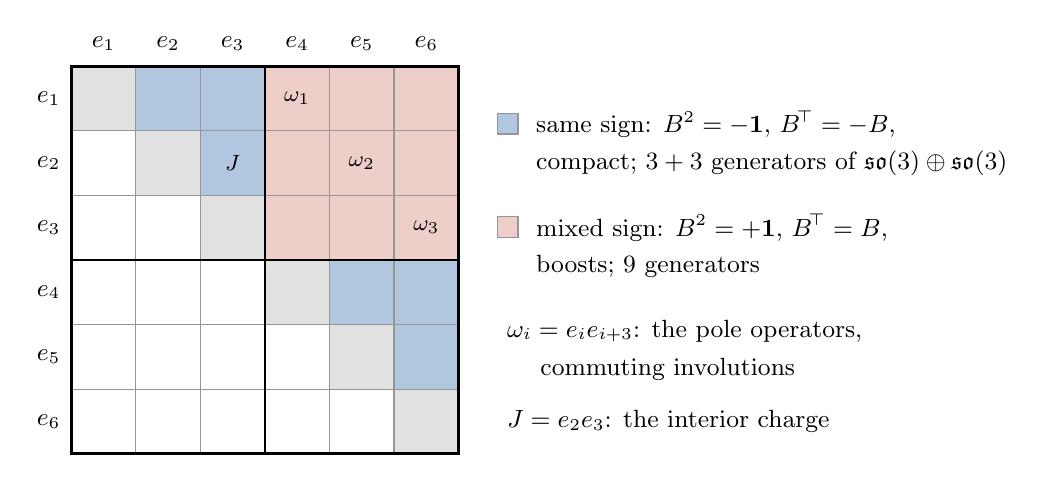
\begin{tikzpicture}[scale=0.82]
\foreach \i in {1,...,6}{
  \node at (\i-0.5,0.35) {\small $e_{\i}$};
  \node at (-0.35,-\i+0.5) {\small $e_{\i}$};
}
\foreach \i in {1,...,6}{
  \foreach \j in {1,...,6}{
    \pgfmathtruncatemacro{\ti}{\i<4 ? 1 : 0}
    \pgfmathtruncatemacro{\tj}{\j<4 ? 1 : 0}
    \ifnum\j>\i
      \ifnum\ti=\tj
        \fill[tcol!35] (\j-1,-\i+1) rectangle (\j,-\i);
      \else
        \fill[scol!25] (\j-1,-\i+1) rectangle (\j,-\i);
      \fi
    \fi
    \ifnum\j=\i \fill[lgray] (\j-1,-\i+1) rectangle (\j,-\i); \fi
  }
}
\draw[step=1,mgray,thin] (0,-6) grid (6,0);
\draw[very thick] (0,0) rectangle (6,-6);
\draw[thick] (3,0) -- (3,-6); \draw[thick] (0,-3) -- (6,-3);
% pole operators
\foreach \i in {1,2,3}{\pgfmathtruncatemacro{\jj}{\i+3}\node at (\jj-0.5,-\i+0.5) {\footnotesize $\omega_{\i}$};}
\node at (2.5,-1.5) {\footnotesize $J$};
\fill[tcol!35] (6.6,-1.05) rectangle ++(0.32,0.32); \draw[mgray] (6.6,-1.05) rectangle ++(0.32,0.32);
\node[align=left,anchor=west] at (7.05,-0.9) {\small same sign: $B^2=-\id$, $B^{\!\top}=-B$,};
\node[align=left,anchor=west] at (7.05,-1.5) {\small compact; $3+3$ generators of $\so3\oplus\so3$};
\fill[scol!25] (6.6,-2.65) rectangle ++(0.32,0.32); \draw[mgray] (6.6,-2.65) rectangle ++(0.32,0.32);
\node[align=left,anchor=west] at (7.05,-2.5) {\small mixed sign: $B^2=+\id$, $B^{\!\top}=B$,};
\node[align=left,anchor=west] at (7.05,-3.1) {\small boosts; $9$ generators};
\node[align=left,anchor=west] at (6.6,-4.1) {\small $\omega_i=e_ie_{i+3}$: the pole operators,};
\node[align=left,anchor=west] at (6.6,-4.7) {\small \phantom{$\omega_i$} commuting involutions};
\node[align=left,anchor=west] at (6.6,-5.5) {\small $J=e_2e_3$: the interior charge};
\end{tikzpicture}
\caption{The fifteen bivectors $e_ae_b$, $a<b$, of $\Cl(3,3)$. Blue cells pair two directions of the same sign and generate
compact rotations; red cells pair a temporal with a spatial direction and generate boosts (\cref{thm:sig}). The diagonal of
the red block holds the three pole operators, which grade the algebra (\cref{prop:grading}); the cell $(2,3)$ holds the
bivector $J$ that will become the electromagnetic charge and the imaginary unit.}
\label{fig:bivectors}
\end{figure}

\subsection{The pole operators and a multigrading}
\label{sec:grading}

The mixed bivectors are not idle. The three \emph{pole operators}
\[
\omega_i:=e_ie_{i+3}\qquad(i=1,2,3)
\]
are boosts, so $\omega_i^2=+\id$, and they commute pairwise by \eqref{eq:bladecomm}, since any two share no index. Square
$-\id$ gauges and square $+\id$ grades, and no bivector does both.

\begin{proposition}[A $\Z_2^3$ grading of $\Cl(3,3)$]
\label{prop:grading}
For a blade $e_I$ put $\chi_i(e_I)=(-1)^{|I\cap\{i,i+3\}|}$. Then $\omega_ie_I\omega_i^{-1}=\chi_i(e_I)\,e_I$, and
$\Cl(3,3)=\bigoplus_{\sigma\in\{\pm\}^3}\Cl_\sigma$ is a multiplicative grading with eight sectors of dimension eight.
\begin{enumerate}[label=(\roman*),leftmargin=2.2em]
\item The joint spectrum of $(\omega_1,\omega_2,\omega_3)$ on $S$ consists of all eight sign triples, each on a line, so the
pole operators cut $\R^8$ into eight one-dimensional eigenlines.
\item The vectors occupy the three weights with exactly one minus sign, two each ($e_i$ and $e_{i+3}$); the bivectors occupy
the four even weights with multiplicities $3,4,4,4$; the all-minus weight is spanned by eight trivectors, namely $e_1e_2e_3$,
$e_4e_5e_6$ and six mixed ones.
\item Correspondingly $\so{3,3}=\mathfrak g_0\oplus\mathfrak g_1\oplus\mathfrak g_2\oplus\mathfrak g_3$ is graded by the Klein
four-group, of dimensions $3+4+4+4$, with $\mathfrak g_0=\operatorname{span}\{\omega_1,\omega_2,\omega_3\}$ abelian,
self-normalising and consisting of semisimple elements with real eigenvalues: a maximally split Cartan subalgebra of
$\so{3,3}\cong\slr{4,\R}$.
\end{enumerate}
\end{proposition}

\begin{proof}
The conjugation sign is \eqref{eq:bladecomm} with $|J|=2$: $(-1)^{2|I|-|I\cap\{i,i+3\}|}$. The weight is multiplicative because
$|I\triangle I'|$ and $|I|+|I'|$ have the same parity in each pair. The census in (ii) is a count of how many generators of
each pair a blade contains. For (iii), a bivector inside one pair is a pole operator, of weight $(+,+,+)$; a bivector with one
generator in each of two pairs has two minus signs, and each of the three such weights holds $2\times2=4$ bivectors. The
pole operators commute, are symmetric with eigenvalues $\pm1$, and the centraliser of $\mathfrak g_0$ in $\so{3,3}$ is
$\mathfrak g_0$ itself, because every other bivector has a nontrivial weight; its dimension equals the real rank three of
$\so{3,3}$.
\end{proof}

The three characters are grading weights, not metric signatures: $e_1$ and $e_4$ carry the same weight and opposite squares,
so nothing in the grading tells a temporal from a spatial direction. The decomposition in (iii) is the root decomposition of
$\slr{4,\R}$ with respect to a split Cartan subalgebra, grouped by the root lattice modulo two; gradings of Clifford and
classical Lie algebras by $\Z_2^n$ are well known \cite{MosnaMirallesVaz}, and we use this one because the pole operators will
reappear in the field-strength reading as the six planes $(e_i,e_{i+3})$ that carry one complex component each.

\begin{example}[The paired-mode projector]
\label{ex:pairedmode}
Let $\mathsf P=\omega_1+\omega_2+\omega_3$ be the sum of the pole operators and $\mathcal V=e_1e_2\cdots e_6$. On the joint
eigenline of signs $(\varepsilon_1,\varepsilon_2,\varepsilon_3)$, $\mathsf P=\varepsilon_1+\varepsilon_2+\varepsilon_3\in\{3,1,-1,-3\}$
with multiplicities $1,3,3,1$. Reordering $\omega_1\omega_2\omega_3=e_1e_4e_2e_5e_3e_6$ into $e_1\cdots e_6$ costs three
transpositions, so $\mathcal V=-\varepsilon_1\varepsilon_2\varepsilon_3$ on that line. Hence $\tfrac12(\mathsf P+\mathcal V)$ takes the
values $1,1,-1,-1$ on the four strata: it is the sign of $\mathsf P$, and equals the polynomial $(13\mathsf P-\mathsf P^3)/12$.
The operator
\begin{equation}
\label{eq:Piclosed}
\Pi:=\tfrac12\id-\tfrac14(\mathsf P+\mathcal V)
\end{equation}
is therefore the orthogonal projector of rank four onto the strata with $\mathsf P<0$. We call it the paired-mode projector; it
is a natural candidate for an observation projector at one constituent and we test it against the photon in
\cref{sec:photon}.
\end{example}

\subsection{The interior four-plane and the surplus plane}
\label{sec:interior}

The physical reading of the arena singles out a Lorentzian four-plane inside $V$. We take
\[
E=\langle e_1,e_4,e_5,e_6\rangle,\qquad \gamma^0=e_1,\quad \gamma^a=e_{a+3}\ (a=1,2,3),
\]
of signature $(1,3)$, and call the orthogonal complement $U=\langle e_2,e_3\rangle$ the surplus plane. The interior Lorentz
algebra $\lint$ is spanned by the six bivectors of $E$, with rotations $S_1=\tfrac12\gamma^2\gamma^3$ (cyclically) and boosts
$T_a=\tfrac12\gamma^0\gamma^a$. Its spin Casimir on $S$ is $-\sum_aS_a^2=\tfrac34\id$, and a rotation through $2\pi$ is $-\id$
on $S$ while it is $+\id$ on vectors (\cref{sec:spin}): the same rotors give spin one-half to spinors and spin one to vectors.

\begin{proposition}[The interior charge is unique]
\label{prop:6plus8plus1}
As $\lint$-modules, $\Lambda^2V=\Lambda^2E\oplus(E\otimes U)\oplus\Lambda^2U$, of dimensions $6+8+1$, is the adjoint
representation, two copies of the vector representation, and the trivial representation. The centraliser of $\lint$ in
$\so{3,3}$ is therefore the line spanned by
\[
J:=e_2e_3 ,
\]
which satisfies $J^2=-\id$, $J^{\!\top}=-J$, and commutes with each of the four gamma matrices.
\end{proposition}

\begin{proof}
The adjoint and vector representations of $\so{1,3}$ contain no invariant, so only $\Lambda^2U$ survives. That $J$ commutes
with $e_1,e_4,e_5,e_6$ is \eqref{eq:bladecomm} with disjoint index sets and $|I||J|=2$.
\end{proof}

\begin{figure}[t]
\centering
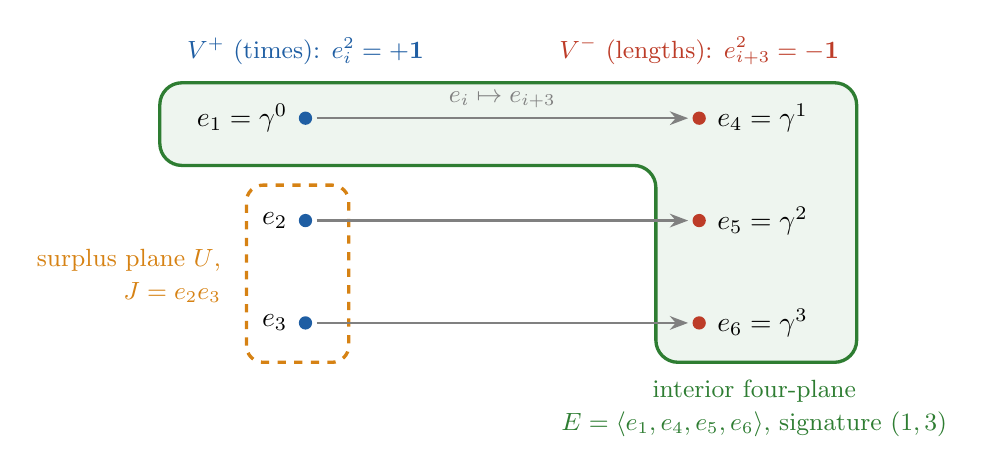
\begin{tikzpicture}[>=Stealth]
\coordinate (t1) at (0,2.6); \coordinate (t2) at (0,1.3); \coordinate (t3) at (0,0);
\coordinate (s1) at (5,2.6); \coordinate (s2) at (5,1.3); \coordinate (s3) at (5,0);
% interior four-plane (L-shaped region)
\fill[gcol!8,rounded corners=8pt] (-1.85,3.05) -- (7.0,3.05) -- (7.0,-0.5) -- (4.45,-0.5) -- (4.45,2.0) -- (-1.85,2.0) -- cycle;
\draw[gcol,very thick,rounded corners=8pt] (-1.85,3.05) -- (7.0,3.05) -- (7.0,-0.5) -- (4.45,-0.5) -- (4.45,2.0) -- (-1.85,2.0) -- cycle;
% surplus plane
\draw[ocol,very thick,dashed,rounded corners=6pt] (-0.75,-0.5) rectangle (0.55,1.75);
% pairing arrows
\draw[->,gray,thick,shorten <=4pt,shorten >=4pt] (t1) -- node[above] {\small $e_i\mapsto e_{i+3}$} (s1);
\draw[->,gray,thick,shorten <=4pt,shorten >=4pt] (t2) -- (s2);
\draw[->,gray,thick,shorten <=4pt,shorten >=4pt] (t3) -- (s3);
\foreach \p in {t1,t2,t3}{\fill[tcol] (\p) circle (2.4pt);}
\foreach \p in {s1,s2,s3}{\fill[scol] (\p) circle (2.4pt);}
\node[left=3pt] at (t1) {$e_1=\gamma^0$}; \node[left=3pt] at (t2) {$e_2$}; \node[left=3pt] at (t3) {$e_3$};
\node[right=3pt] at (s1) {$e_4=\gamma^1$}; \node[right=3pt] at (s2) {$e_5=\gamma^2$}; \node[right=3pt] at (s3) {$e_6=\gamma^3$};
\node[tcol,anchor=south] at (0,3.15) {\small $V^+$ (times): $e_i^2=+\id$};
\node[scol,anchor=south] at (5,3.15) {\small $V^-$ (lengths): $e_{i+3}^2=-\id$};
\node[ocol,anchor=east,align=right] at (-0.95,0.6) {\small surplus plane $U$,\\ \small $J=e_2e_3$};
\node[gcol,anchor=north,align=center] at (5.7,-0.6) {\small interior four-plane\\ \small $E=\langle e_1,e_4,e_5,e_6\rangle$, signature $(1,3)$};
\end{tikzpicture}
\caption{The arena. The positive triple $V^+$ (times) and the negative triple $V^-$ (lengths) are paired by $e_i\mapsto e_{i+3}$;
the pairing has two square roots, the grading $\cK$ and the binding operator $G$ (\cref{prop:twoK}). The interior four-plane
$E$, on which the Dirac sector is built, contains the clock $e_1$ and the whole spatial triple; its complement is the surplus
plane $U=\langle e_2,e_3\rangle$, whose rotation generator $J$ is the only bivector commuting with the interior Lorentz algebra
(\cref{prop:6plus8plus1}).}
\label{fig:arena}
\end{figure}

\Cref{prop:6plus8plus1} is the first instance of a pattern that recurs throughout: a structure is fixed once the right
ambient algebra and the right conditions are named, and it ceases to be fixed when either is relaxed. Here the ambient
space is the span of the bivectors and the condition is commutation with $\lint$. In \cref{sec:dirac} we enlarge the ambient
algebra to all of $\End_\R(S)$ and find that a different condition, commutation with the internal bivectors, is what keeps the
answer unique.

\section{Time, conversion, and the two square roots of the pairing}
\label{sec:clock}

\subsection{One conversion constant}

The split form is not dimensionally innocent. If $V^+$ carries times and $V^-$ lengths, then
$\eta(v,v)=\sum_i(t^i)^2-\sum_a(x^a)^2$ adds squared times to squared lengths, and a conversion is needed, a priori one
constant for each temporal axis.

\begin{proposition}[A pairing alone does not give isotropy]
\label{prop:KC}
A map exchanging $V^+$ and $V^-$ cannot carry a single dimension; it converts times to lengths one way and lengths to times
the other. In block form
\begin{equation}
\label{eq:KC}
\cK_C=\begin{pmatrix}0&C^{-1}\\ C&0\end{pmatrix},\qquad C:V^+\to V^-,\qquad [C]=LT^{-1},
\end{equation}
one has $\cK_C^2=\id$ for every invertible $C$, including $C=\operatorname{diag}(c_1,c_2,c_3)$ with distinct entries. An
involutive pairing therefore does not force $c_1=c_2=c_3$.
\end{proposition}

\begin{theorem}[One conversion constant]
\label{thm:onec}
If a common $SO(3)$ acts on $V^+$ and on $V^-$ by the vector representation and $C$ intertwines the two actions, then
$C=c\,\id$ with $[c]=LT^{-1}$.
\end{theorem}

\begin{proof}
The vector representation of $SO(3)$ is irreducible of real type, so its commutant is $\R$ and Schur's lemma places $C$ in
$\R\,\id$ \cite{GoodmanWallach}.
\end{proof}

\subsection{The two square roots of the pairing}

Dimensional analysis fixes $[C]$ and leaves the sign of the lower-left block free. The two choices are different operators,
and the rest of the paper turns on the difference.

\begin{proposition}[The grading root and the binding root]
\label{prop:twoK}
In units with $c=1$, and in block form on $V^+\oplus V^-$, put
\[
\cK=\begin{pmatrix}0&-\id\\ -\id&0\end{pmatrix},\qquad
G=\begin{pmatrix}0&-\id\\ \id&0\end{pmatrix},
\]
that is $\cK e_i=-e_{i+3}$, $\cK e_{i+3}=-e_i$, and $Ge_i=e_{i+3}$, $Ge_{i+3}=-e_i$. Then:
\begin{center}
\begin{tabular}{@{}lcccl@{}}
\toprule
& square & $\eta$-adjoint & $\eta(X\cdot,X\cdot)$ & role\\
\midrule
$\cK$ & $+\id$ & $\cK^\dagger=-\cK$ & $-\eta$ & an element of $\so{3,3}$; grades\\
$G$ & $-\id$ & $G^\dagger=+G$ & $-\eta$ & a complex structure outside $\so{3,3}$; binds\\
\bottomrule
\end{tabular}
\end{center}
with $X^\dagger:=\eta^{-1}X^{\!\top}\eta$. Both are anti-isometries. The eigenspaces of $\cK$ are the two totally null three-planes
spanned by $e_i\mp e_{i+3}$.
\end{proposition}

Both roots can be built inside the algebra, and they are related by a single trivector.

\begin{lemma}[Both roots from Clifford data]
\label{lem:Gclifford}
Let $\mathsf P=\sum_i e_ie_{i+3}$ and $T=e_1e_2e_3$, and define $\cK(v)=\tfrac12[\mathsf P,v]$ and $S(v)=TvT^{-1}$ on vectors. Then
$\cK(e_i)=-e_{i+3}$, $\cK(e_{i+3})=-e_i$, so $\cK^2=\id$; $S$ fixes the temporal and negates the spatial generators, so $S=\eta$ as a
map of $V$; and
\[
G=-\cK\circ S .
\]
\end{lemma}

\begin{proof}
$[e_ie_{i+3},e_i]=e_ie_{i+3}e_i-e_i^2e_{i+3}=-2e_{i+3}$ and $[e_ie_{i+3},e_{i+3}]=e_ie_{i+3}^2-e_{i+3}e_ie_{i+3}=-2e_i$, while the
other pole operators commute with both by \eqref{eq:bladecomm}. $T$ is a product of the three temporal generators, so it
commutes with each of them up to the sign $(-1)^{3-1}=+1$ and anticommutes with each spatial generator. Finally
$-\cK(S e_i)=-\cK(e_i)=e_{i+3}=Ge_i$ and $-\cK(Se_{i+3})=\cK(e_{i+3})=-e_i=Ge_{i+3}$.
\end{proof}

So the root that grades is $\tfrac12\ad_{\mathsf P}$, the adjoint action of the sum of the pole operators, and the root that binds
is the same map composed with the Cartan involution $S=\Ad_{e_1e_2e_3}$. That the two roots are distinguished exactly by the
Cartan involution is the cleanest single statement the flat and the curved analyses below jointly support.

\paragraph{Shift operators.} A clock coordinate $\lambda$ has dimension $T$, the operator $G$ is dimensionless, and their sum
requires a scale. With a length $\ell$,
\begin{equation}
\label{eq:kappa}
\kappa=\frac c\ell,\qquad \alpha_\pm=\partial_\lambda\pm\kappa G .
\end{equation}
The pointwise $\eta$-adjoint of $\kappa G$ is $\kappa G$, while the formal adjoint of the differential operator, after an integration by
parts with compatible boundary conditions, is $(\partial_\lambda+\kappa G)^*=-\partial_\lambda+\kappa G^\dagger=-\alpha_-$. The two
adjoints must be kept apart: the factorisations below are insensitive to the overall sign, positivity statements are not.

\subsection{The clock}
\label{sec:clocksimplex}

A clock is a unit vector of $V^+$. Which one? Let $w=(w_1,w_2,w_3)$ be normalised non-negative weights on the three temporal
axes, so that $w$ ranges over the two-simplex $\Delta^2$. The map $x_i=2\sqrt{w_i}$ sends $\Delta^2$ onto the part of the sphere
$\sum_ix_i^2=4$ in the closed positive octant, and since $dx_i=dw_i/\sqrt{w_i}$ the Euclidean metric pulls back to
\[
\sum_idx_i^2=\sum_i\frac{dw_i^2}{w_i},
\]
the Fisher--Rao metric. That metric is not a modelling choice: by \v{C}encov's theorem it is, up to scale, the only metric on a
finite simplex invariant under Markov morphisms \cite{Cencov,AmariNagaoka}. The space of clocks is therefore an octant of a round
sphere of radius two.

\begin{proposition}[The symmetric clock]
\label{prop:clock}
The barycentre $w=(\tfrac13,\tfrac13,\tfrac13)$ is the unique point of $\Delta^2$ fixed by the permutations of the three axes, and the
unique maximum of the entropy $-\sum_iw_i\log w_i$, with value $\log3$ and Hessian eigenvalues $-9$ and $-3$ in the chart
$(w_1,w_2)$. Its amplitude direction is the unit vector
\[
\widehat W=\frac{e_1+e_2+e_3}{\sqrt3},\qquad \widehat W^2=\id,\qquad
\lambda:=\eta(\widehat W,v)=\frac{t^1+t^2+t^3}{\sqrt3}=\sqrt3\,\bar t .
\]
\end{proposition}

The permutation argument carries the weight here; the entropy argument is Jaynes' principle and is a hypothesis, recorded as
such. What the proposition says is modest: if a clock is to treat the three temporal axes alike, it is $\widehat W$, and the
physical time it reads is $\sqrt3$ times the mean of the three constituent times. It does not say that $\lambda$ is a proper time,
that it is invariant under a group, or that the directions orthogonal to $\widehat W$ are unphysical. Those directions,
$\widehat W^\perp\cap V^+=\{t^1+t^2+t^3=0\}$, spanned by $e_1-e_2$ and $e_1+e_2-2e_3$, are the \emph{relative times}.

\begin{figure}[t]
\centering
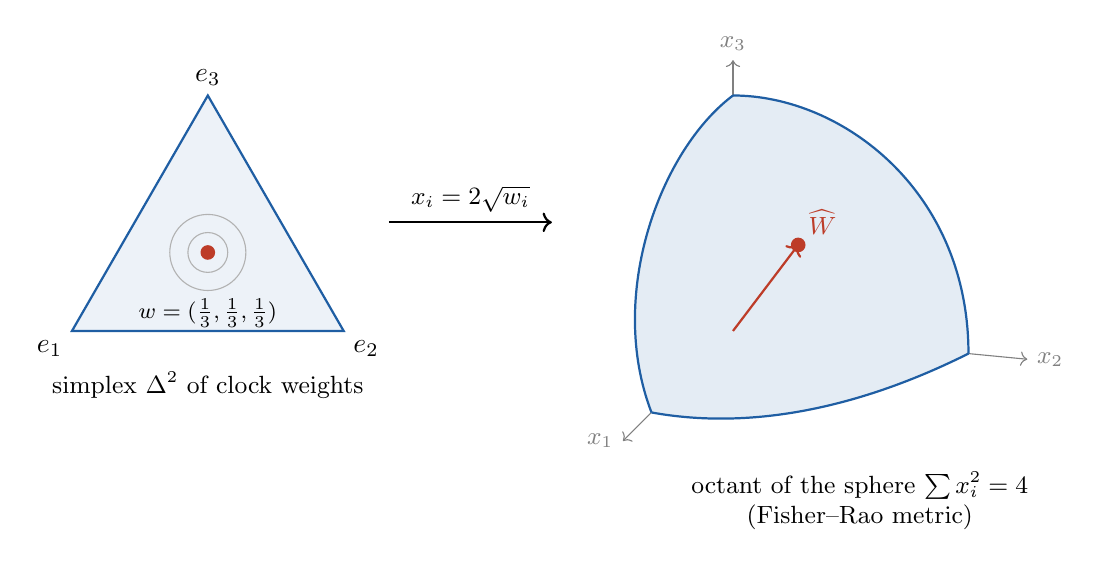
\begin{tikzpicture}[scale=1.15]
% simplex
\begin{scope}
\coordinate (A) at (0,0); \coordinate (B) at (3,0); \coordinate (Cc) at (1.5,2.6);
\fill[tcol!8] (A)--(B)--(Cc)--cycle; \draw[tcol,thick] (A)--(B)--(Cc)--cycle;
\node[below left] at (A) {$e_1$}; \node[below right] at (B) {$e_2$}; \node[above] at (Cc) {$e_3$};
\coordinate (bar) at (1.5,0.8667);
\fill[scol] (bar) circle (2.3pt);
\node at (1.5,0.2) {\footnotesize $w=(\tfrac13,\tfrac13,\tfrac13)$};
\foreach \r in {0.22,0.42}{\draw[gray!60,thin] (bar) circle (\r);}
\node at (1.5,-0.6) {\small simplex $\Delta^2$ of clock weights};
\end{scope}
\draw[->,thick] (3.5,1.2) -- node[above] {\small $x_i=2\sqrt{w_i}$} (5.3,1.2);
% octant of sphere, drawn in an oblique projection
\begin{scope}[shift={(7.3,0)}]
\coordinate (O) at (0,0);
\coordinate (X) at (2.6,-0.25); \coordinate (Y) at (-0.9,-0.9); \coordinate (Z) at (0,2.6);
\draw[->,gray] (O)--($1.25*(X)$) node[right] {\small $x_2$};
\draw[->,gray] (O)--($1.35*(Y)$) node[left] {\small $x_1$};
\draw[->,gray] (O)--($1.15*(Z)$) node[above] {\small $x_3$};
\fill[tcol!12] (X) .. controls ($(X)+(0,1.8)$) and ($(Z)+(1.2,0)$) .. (Z)
  .. controls ($(Z)+(-0.8,-0.6)$) and ($(Y)+(-0.5,1.3)$) .. (Y)
  .. controls ($(Y)+(1.1,-0.2)$) and ($(X)+(-1.2,-0.6)$) .. (X);
\draw[tcol,thick] (X) .. controls ($(X)+(0,1.8)$) and ($(Z)+(1.2,0)$) .. (Z);
\draw[tcol,thick] (Z) .. controls ($(Z)+(-0.8,-0.6)$) and ($(Y)+(-0.5,1.3)$) .. (Y);
\draw[tcol,thick] (Y) .. controls ($(Y)+(1.1,-0.2)$) and ($(X)+(-1.2,-0.6)$) .. (X);
\coordinate (Wp) at (0.72,0.95);
\fill[scol] (Wp) circle (2.3pt);
\draw[->,scol,thick] (O) -- (Wp) node[above right] {\small $\widehat W$};
\node[align=center,anchor=north] at (1.4,-1.45) {\small octant of the sphere $\sum x_i^2=4$\\[-1pt] \small (Fisher--Rao metric)};
\end{scope}
\end{tikzpicture}
\caption{The space of clocks. Normalised weights on the three temporal axes form a simplex; the amplitude map carries it onto an
octant of a round sphere, whose round metric is the Fisher--Rao metric. The barycentre, the only permutation-invariant point and
the entropy maximum, corresponds to the symmetric clock $\widehat W=(e_1+e_2+e_3)/\sqrt3$ (\cref{prop:clock}).}
\label{fig:clock}
\end{figure}

\subsection{The spectrum of a conversion operator}

An operator that converts times into lengths is a mixed bivector $B_C=\sum_{i,a}C_{ia}\,e_ie_{a+3}$, symmetric by
\cref{thm:sig}. Its square controls the factorised interior dynamics of \cref{sec:shifted}, where the equation of motion becomes
$\ddot X=\kappa^2B_C^2X$, so its spectrum is worth knowing exactly.

\begin{theorem}[Spectrum of a conversion operator]
\label{thm:spectrumBC}
Write $C=\sum_k\sigma_ku_kv_k^{\!\top}$ in singular-value form and put $U_k=\sum_iu_k^ie_i$, $V_k=\sum_av_k^ae_{a+3}$ and
$B_k=U_kV_k$. Then $B_k^2=\id$, the $B_k$ commute, and
\[
B_C^2=\|C\|_F^2\,\id+2\sum_{k<l}\sigma_k\sigma_l\,\Omega_{kl},\qquad \Omega_{kl}=B_kB_l,\qquad \Omega_{12}\Omega_{13}=\Omega_{23}.
\]
Consequently
\[
\spec\bigl(B_C^2\bigr)=\bigl\{(\eta_1\sigma_1+\eta_2\sigma_2+\eta_3\sigma_3)^2:\ \eta\in\{\pm1\}^3\bigr\},
\]
four values, each of multiplicity two on $\R^8$.
\end{theorem}

\begin{proof}
$U_k$ and $V_k$ are orthogonal unit vectors of square $+\id$ and $-\id$, so $B_k^2=-U_k^2V_k^2=\id$; for $k\neq l$ the four vectors
$U_k,V_k,U_l,V_l$ are mutually orthogonal and $B_k,B_l$ commute by \eqref{eq:bladecomm}. Expanding the square gives the formula. The
seven nontrivial products of the commuting involutions $B_k$ are, in a rotated orthonormal basis of $V$, blades of grade two, four
or six, hence traceless; the joint eigenspace with signs $\eta$ therefore has dimension $\tfrac18\Tr\prod_k(\id+\eta_kB_k)=1$, and on it
$B_C=\eta\cdot\sigma$.
\end{proof}

\begin{corollary}[Rank counts clocks]
\label{cor:rankclock}
$B_C^2$ is a multiple of $\id$ if and only if $\rank C\le1$, and some eigenvalue of $B_C^2$ vanishes if and only if one singular value
equals the sum of the other two. The rank of $C$ is the number of independent temporal directions the conversion uses.
\end{corollary}

\begin{example}[The symmetric clock is dynamically blind]
\label{ex:blindclock}
The operators $G_a:=\widehat W e_{a+3}$, which convert along the symmetric clock, have $C=\widehat W\hat e_a^{\!\top}$ of rank one and
singular values $(1,0,0)$. Hence $G_a^2=\id$, the factorised equation of motion is $\ddot X=\kappa^2X$, and the conversion operator does not
appear in it at all. The clock singled out by the symmetry is exactly the clock whose dynamics cannot see the Clifford structure. This is
forced by the rank: if every left singular vector of $C$ is proportional to $\widehat W$, then $C$ has rank one. A conversion visible in the
equations of motion therefore needs a temporal direction transverse to $\widehat W$, that is, a relative time. Raising the rank does not
produce oscillation either: the eigenvalues $(\eta\cdot\sigma)^2$ are real and non-negative at every rank, so higher rank makes the
instability anisotropic, with four rates $\kappa|\eta\cdot\sigma|$ instead of one, and can create flat directions, but never a bounded
oscillation. Bounded motion has to come from elsewhere, and \cref{sec:neutral} shows where.
\end{example}

\section{The imaginary unit and the Dirac structure}
\label{sec:dirac}

\subsection{The complex structure is selected}

At $n$ constituents write $\Omega=\gamma^0\gamma^1\gamma^2\gamma^3=e^{(1)}_1e^{(1)}_4e^{(1)}_5e^{(1)}_6$ for the volume element of the
interior four-plane and $\wI$ for the product, in increasing order, of the remaining $6n-4$ generators, the \emph{internal}
directions. At $n=1$ these are $e_2,e_3$ and $\wI=e_2e_3=J$.

\begin{theorem}[Selection of the imaginary unit]
\label{thm:i}
Inside $\End_\R(S_n)$ the joint commutant of the interior Lorentz algebra and of all internal bivectors is
$\operatorname{span}\{\id,\Omega,\wI,\Omega\wI\}\cong\C\otimes_\R\C\cong\C\oplus\C$, at every rung. Its solutions of
$x^2=-\id$ are the four isolated points $\pm\Omega$, $\pm\wI$. Of these only $\pm\wI$ commute with the interior gamma
matrices, from which the kinetic operator is built. Hence the imaginary unit is $i=\pm\wI$, and the chirality is
$\gamma_5=\mp\Omega\wI=\mp\Gamma$ with
\[
\Gamma:=\wI\,\Omega,\qquad \Gamma^2=\id .
\]
\end{theorem}

\begin{proof}
By \eqref{eq:bladecomm}, commuting with the six interior bivectors and with every internal bivector is a parity condition on
each blade, and the blades that satisfy all of them are exactly the four listed, at every rung. A four-dimensional
commutative real algebra with two commuting square roots of $-\id$ and no nilpotents is $\C\oplus\C$, whose square roots of
$-1$ are those four points. Finally $\Omega$ is the product of the four interior generators, so it anticommutes with each of
them, while $\wI$ contains no interior index and commutes with each.
\end{proof}

From now on $J$ denotes $\wI$; at one constituent this is $e_2e_3$, the generator of \cref{prop:6plus8plus1}. The selection
depends on its conditions, and it is worth saying exactly how.

\begin{remark}[The ambient algebra is part of the statement]
\label{rem:ambient}
If commutation with the internal bivectors is dropped, then at $n=1$ the commutant of the four gamma matrices in $M_8(\R)$ is the
quaternion algebra
\[
\HH=\operatorname{span}\{\id,\ J,\ e_2\Omega,\ e_3\Omega\},
\]
and its square roots of $-\id$ form a two-sphere. One further datum removes that freedom. The volume element of the temporal triple,
$T:=e_1e_2e_3$, depends only on the splitting $V=V^+\oplus V^-$ and on an orientation of $V^+$; it commutes with $J$ and anticommutes
with $e_2\Omega$ and $e_3\Omega$ by \eqref{eq:bladecomm}, so
\[
\{X\in\HH:\ [X,T]=0\}=\R\,\id\oplus\R\,J ,
\]
and $J=\gamma^0T$ is recovered from the clock and the temporal orientation, up to the sign of that orientation. Higher up the
tower the commutant of the gamma matrices alone acquires a matrix multiplicity algebra; at $n=3$ the Lorentz commutant is
$M_{128}(\C)$, whose own complex structure is $\Omega$ and not $\wI$ (\cref{prop:config}). Selection tracks the conditions imposed,
and every uniqueness statement in this paper is made with them.
\end{remark}

That the imaginary unit is not adjoined but read off the algebra is the cleanest structural result at one constituent. It has an
independent counterpart: on a real Hilbert space, Poincar\'e symmetry alone can force the complex structure \cite{MorettiOppio}.

\subsection{Real Dirac theory is complex Dirac theory}

\begin{theorem}[Exactness of the realification]
\label{thm:realification}
The $\C$-linear algebra generated by the interior gamma matrices on $(S,J)\cong\C^4$ is all of $M_4(\C)$. Consequently the real
Maxwell--Dirac system on $\Cl(3,3)$ is ordinary complex Maxwell--Dirac theory written in real variables.
\end{theorem}

\begin{proof}
$J$ commutes with the four $\gamma^\mu$. The sixteen monomials in the $\gamma^\mu$ and their $J$-multiples are thirty-two
linearly independent real matrices commuting with $J$, and the commutant of $J$ in $M_8(\R)$ is $\End_\C(\C^4)=M_4(\C)$, of real
dimension thirty-two.
\end{proof}

\begin{corollary}
\label{cor:nopredict}
Anything derivable from the real formulation alone was derivable from the complex one, and conversely. The gauged system is quantum
electrodynamics in real variables, and no prediction can follow from the rewriting.
\end{corollary}

This is the deflationary principle of the introduction. It does not make the arena uninteresting; it says where its content can
lie. Everything below that depends only on the four gamma matrices and $J$ is inherited. What is not inherited is what the arena
adds: the selection of $J$, the surplus plane and its uses, the pairing, and the tower.

\subsection{Admissible bilinears}

A field $\psi$ with values in $S$ is real. If its components anticommute, a term $\psi^{\!\top}A\psi$ vanishes when $A$ is
symmetric, and $\psi^{\!\top}A\,\partial\psi=\tfrac12\partial(\psi^{\!\top}A\psi)$ is a total derivative when $A$ is antisymmetric. A
mass term therefore needs an antisymmetric kernel, and a first-order kinetic term a symmetric one. With the clock $\gamma^0=e_1$:

\begin{proposition}[Kernels of fixed symmetry]
\label{prop:kernels1}
The mass form $\gamma^0J$ is antisymmetric. The kinetic kernels
\[
K^\mu:=(\gamma^0J)(J\gamma^\mu)=-\gamma^0\gamma^\mu,\qquad K^0=-\id,
\]
are symmetric, while $(\gamma^0J)\gamma^\mu$ is antisymmetric. The kinetic form must therefore carry the factor $J$: its $J$-free analogue
defines a total derivative and constrains nothing a field equation sees.
\end{proposition}

The mass form $\gamma^0J=e_1e_2e_3=T$ is the temporal volume element of \cref{rem:ambient}. It is not the only admissible mass.

\begin{proposition}[Scalar and pseudoscalar mass]
\label{prop:massangle}
The antisymmetric elements of $M_8(\R)$ that commute with $J$ and are invariant under the interior Lorentz algebra form the
two-dimensional space $\operatorname{span}\{T,\ T\Omega\}$. Used as the kernel of the Dirac bilinear, the second contributes nothing
to the kinetic term, because $T\Omega J\gamma^\mu$ is antisymmetric for every $\mu$; the two differ only in the mass term. $T$ is a
scalar mass and $T\Omega$ a pseudoscalar one, since $\Omega^2=-\id$ and $\Omega$ anticommutes with every $\gamma^\mu$, so that $\Omega$
is the real form of $i\gamma_5$. The family $T(\cos\vartheta+\sin\vartheta\,\Omega)=Te^{\vartheta\Omega}$ is the chiral mass angle.
\end{proposition}

So $T$ is singled out among admissible masses by the requirement that the mass be scalar, and that requirement is an input. The
central element $\Omega$ will reappear in \cref{sec:discrete} as the axial $U(1)$.

\paragraph{The Hamiltonian.} The free Dirac Hamiltonian at momentum $p$ is
\begin{equation}
\label{eq:Hp}
H(p)=\gamma^0\gamma^ap_a+m\gamma^0,\qquad H(p)^2=E^2\id,\qquad E^2=|\bp|^2+m^2 ,
\end{equation}
with spectral projectors $\Lambda_\pm(p)=\tfrac12(\id\pm H(p)/E)$. Both $\gamma^0=e_1$ and $\gamma^0\gamma^a=e_1e_{a+3}$ are symmetric, so
$H(p)$ is a symmetric matrix that commutes with $J$; its eigenvalues are $\pm E$, each with real multiplicity four.

\begin{example}
\label{ex:Hp}
At $\bp=(0,0,3)$ and $m=4$, $H=3e_1e_6+4e_1$ satisfies $H^2=(9+16)\id=25\,\id$, because $e_1e_6$ and $e_1$ anticommute and
$(e_1e_6)^2=+\id$. The eigenvalues are $\pm5$; each eigenspace is a complex plane for $J$, and the helicity
$\Sigma_3=J\,\tfrac12e_4e_5$ commutes with $H$ and splits each of them into two real planes.
\end{example}

\subsection{A first-order real form of free evolution}

For a commuting real field the same data give a first-order symplectic system. Take
\[
\cL_1=\tfrac12\Psi^{\!\top}J\dot\Psi-\tfrac12\Psi^{\!\top}H(p)\Psi .
\]
Its Euler--Lagrange equation is $\dot\Psi=-JH(p)\Psi$. Since $JH$ is antisymmetric with $(JH)^2=-E^2\id$, the flow lies in $SO(8)$ and
\[
\Psi(\lambda)=\cos(E\lambda)\,\Psi_0-\frac{\sin(E\lambda)}{E}\,JH\Psi_0 .
\]
Reading $J$ as $i$ turns this into $i\dot\psi=h\psi$ with $h=\alpha\cdot\bp+\beta m$, the free Dirac Hamiltonian at fixed momentum: an exact
embedding of free Dirac evolution in a real symplectic form, with eight second-class constraints reducing a sixteen-dimensional phase
space to eight. Three things norm conservation does not buy. The energy $\tfrac12\Psi^{\!\top}H\Psi$ is unbounded below, since $\Tr H=0$
and $H^2=E^2\id$ force the spectrum $\{\pm E\}$ with equal multiplicity. For anticommuting components the action collapses to a boundary
term, $\Psi^{\!\top}H\Psi=0$ because $H$ is symmetric and $\Psi^{\!\top}J\dot\Psi=\tfrac12\tfrac{d}{d\lambda}(\Psi^{\!\top}J\Psi)$ because $J$ is
antisymmetric, which is why a fermionic Lagrangian must use the kernels of \cref{prop:kernels1}. And the bilinear $\Psi^{\!\top}J\dot\Psi$
is not preserved by the boosts. The real form of Dirac theory in which a bivector commuting with the gamma matrices plays the role of $i$
is old \cite{Hestenes67}; what is specific here is that the bivector is the surplus rotation $J$, selected by \cref{thm:i}.

\section{Discrete symmetries, the massless gauge algebra, and the states}
\label{sec:discrete}

\subsection{Charge conjugation, parity and time reversal}

At one constituent write $U=\langle e_2,e_3\rangle$ for the surplus plane, $\Omega=\gamma^0\gamma^1\gamma^2\gamma^3$, and
$\Gamma=J\Omega$. An operator $X$ on $S$ is \emph{linear} when $XJ=JX$ and \emph{antilinear} when $XJ=-JX$. It intertwines the free
Dirac operator $J\gamma^\mu\partial_\mu-m$ when it commutes with every $J\gamma^\mu$. Parity is required to be linear and time
reversal antilinear, and each must satisfy $XH(p)X^{-1}=H(-p)$ for every $p$ and $m$.

\begin{theorem}[Charge conjugation is the surplus plane]
\label{thm:C}
The antilinear operators that intertwine the Dirac operator form exactly the two-dimensional space $U$. Every unit vector $C\in U$
satisfies
\[
CH(p)C^{-1}=-H(-p),\qquad CJC^{-1}=-J,\qquad C\Gamma C^{-1}=-\Gamma,\qquad C\Lambda_+(p)C^{-1}=\Lambda_-(-p),
\]
commutes with every interior Lorentz generator, and preserves the mass form and every kinetic kernel $K^\mu$. Hence $C$ is unique up
to a gauge rotation $e^{\theta J}$, and the operator known as the Majorana real structure is charge conjugation.
\end{theorem}

\begin{proof}
If $XJ=-JX$, then $X(J\gamma^\mu)=(J\gamma^\mu)X$ is equivalent to $X\gamma^\mu=-\gamma^\mu X$. The conditions are linear, and
conjugation by a blade sends every blade to plus or minus itself, so the solution space is spanned by the blades that anticommute
with $J$ and with $e_1,e_4,e_5,e_6$. By \eqref{eq:bladecomm} a blade $e_I$ anticommutes with a vector $e_a$ exactly when
$|I|-[a\in I]$ is odd. For odd $|I|$ this forces $I\subset\{2,3\}$, hence $I=\{2\}$ or $\{3\}$, and both anticommute with $J$. For
even $|I|$ it forces $\{1,4,5,6\}\subset I$, hence $e_I=\Omega$ or $e_1\cdots e_6$, and both commute with $J$. The solutions are
therefore $e_2$ and $e_3$. The listed identities follow from the same rule, since $e_2,e_3$ anticommute with every $\gamma^\mu$, with
$J$ and with $\Gamma$, and commute with every interior bivector.
\end{proof}

\begin{corollary}[Equal mass, equal spin, opposite charge]
$C$ commutes with every generator of the interior Lorentz algebra, so it preserves the Casimir $-\sum_aS_a^2=\tfrac34\id$, and
$(CH(p)C^{-1})^2=E^2\id$. The Majorana condition $\Psi=C\Psi$ makes the current vanish: a particle that is its own antiparticle is
neutral.
\end{corollary}

\begin{theorem}[Parity and time reversal]
\label{thm:PT}
The admissible parities form the space $\langle\gamma^0,\gamma^0J\rangle$, and $P^2=+\id$ holds only at $P=\pm\gamma^0$, while $P=\pm\gamma^0J$
gives $P^2=-\id$. The admissible time reversals form $U\cdot\gamma^1\gamma^2\gamma^3$, so $T=C\gamma^1\gamma^2\gamma^3$ with
\[
T^2=-\id .
\]
The sign is not a convention: $B=\gamma^1\gamma^2\gamma^3$ has $B^2=+\id$ and anticommutes with every vector $C$ of the clock plane, so
$T^2=CBCB=-C^2B^2=-\|C\|^2\id$ for every choice of clock in the positive triple.
\end{theorem}

\begin{theorem}[$CPT$ lies on a circle]
\label{thm:CPT}
The product of the three operators depends on the parity chosen:
\[
P=\gamma^0:\quad CPT=-\Omega,\ (CPT)^2=-\id;\qquad\qquad P=\gamma^0J:\quad CPT=+\Gamma,\ (CPT)^2=+\id .
\]
What is convention-free is the orbit of $\Omega$ under $U(1)_J$, $\theta\mapsto\cos\theta\,\Omega+\sin\theta\,J\Omega$, whose four real points
$\pm\Omega,\pm\Gamma$ are the spacetime pseudoscalar and the chirality.
\end{theorem}

\begin{figure}[t]
\centering
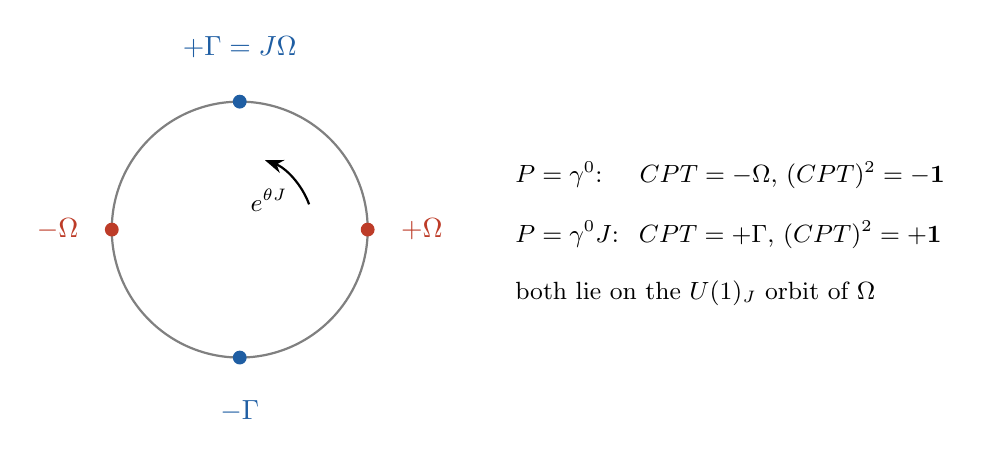
\begin{tikzpicture}[scale=1.25,>=Stealth]
\draw[thick,gray] (0,0) circle (1.3);
\foreach \a/\l/\c in {0/{+\Omega}/scol,90/{+\Gamma=J\Omega}/tcol,180/{-\Omega}/scol,270/{-\Gamma}/tcol}{
  \fill[\c] (\a:1.3) circle (2pt);
  \node[\c] at (\a:1.85) {$\l$};
}
\draw[->,thick] (20:0.75) arc (20:70:0.75);
\node at (45:0.42) {\small $e^{\theta J}$};
\node[align=left,anchor=west] at (2.7,0.55) {\small $P=\gamma^0$: \quad $CPT=-\Omega$,\ $(CPT)^2=-\id$};
\node[align=left,anchor=west] at (2.7,-0.05) {\small $P=\gamma^0J$: \ $CPT=+\Gamma$,\ $(CPT)^2=+\id$};
\node[align=left,anchor=west] at (2.7,-0.65) {\small both lie on the $U(1)_J$ orbit of $\Omega$};
\end{tikzpicture}
\caption{The $CPT$ circle at one constituent (\cref{thm:CPT}). The product of the three discrete operators is the spacetime
pseudoscalar or the chirality according to the parity chosen; the two lie on one orbit of the gauge rotation $e^{\theta J}$.}
\label{fig:cpt}
\end{figure}

These are statements about explicitly constructed operators of the free theory; no $CPT$ theorem is proved, and the interacting
theory is not constructed.

\subsection{The massless gauge algebra at one constituent}

A gauge generator must leave the kinetic form invariant. Solving that condition over all of $\End_\R(S)$, with no ansatz, gives the
following.

\begin{proposition}[Gauge algebra from the kinetic forms]
\label{prop:gauge1}
The solutions of $X^{\!\top}K^\mu+K^\mu X=0$ for $\mu=0,\dots,3$ form
\[
\mathfrak g_{\rm massless}=\R\,\Omega\ \oplus\ \operatorname{span}\{J,\ e_2\Omega,\ e_3\Omega\}\ \cong\ \uu1_\Omega\oplus\su2 .
\]
The condition at $\mu=0$ is $X^{\!\top}=-X$, and the conditions at $\mu=a$ then say that $X$ commutes with the three boosts
$\gamma^0\gamma^a$ and hence with the whole interior Lorentz algebra. The trace form is $-8\,\id$ on this basis, so the algebra is
compact. Adding invariance of the mass form, $X^{\!\top}(\gamma^0J)+(\gamma^0J)X=0$, leaves exactly $\R J$. The algebra meets the span of the
pole operators in zero.
\end{proposition}

The $\su2$ factor contains the fermion-number direction $J$ and two generators that anticommute with $J$; it therefore mixes a field with
its conjugate and is the Pauli--G\"ursey algebra of a massless Dirac field \cite{Pauli57,Gursey58}. It is a symmetry of the free massless
theory, not a gauge candidate on this matter: its two Weyl components form a single doublet, and gauging $SU(2)$ on an odd number of
doublets is forbidden by the global anomaly \cite{Witten82}. The central factor is the axial one. Since $\Gamma=J\Omega$, $\Omega=-J\Gamma$,
which with $i=J$ and the chirality $\gamma_5=-\Gamma$ of \cref{thm:i} is the real form of $i\gamma_5$, as in \cref{prop:massangle}; $U(1)_\Omega$ is broken by a Dirac mass and is anomalous on this matter content \cite{Bilal,AlvarezGaumeWitten}.
The electromagnetic $\uu1$ is therefore singled out twice at one constituent: as the whole internal centraliser
(\cref{prop:6plus8plus1}) and as what survives of the massless gauge algebra once a mass is admitted.

\subsection{The state space}

\begin{theorem}[The real module is not a state space]
\label{thm:module}
Eight $16\times16$ integer matrices $\theta_i$, antisymmetric with $\theta_i^2=-\id$ and pairwise anticommuting, realise the canonical
anticommutation relations of the eight real field components exactly. Their commutant in $M_{16}(\R)$ is $\R\,\id$, because the $256$
Clifford monomials span the whole matrix algebra. Hence no internal complex structure commutes with all eight field operators, and the
quadratic observables built from them are real antisymmetric matrices with imaginary spectra. The quantum state space has to be formed
from outside, as $\mathcal F=\C\otimes_\R\R^{16}$, with charge $Q=-i\rho(J)$ and Hamiltonian $H=-i\rho(JH(p))$, where
$\rho(A)=-\tfrac14\sum_{ij}A_{ij}\theta_i\theta_j$ lifts an antisymmetric $8\times8$ matrix to the module.
\end{theorem}

It is the complex structure, not the reality, that is missing, which is the lesson of \cref{rem:ambient} arriving one level up.

\begin{theorem}[The free spectrum of one momentum]
\label{thm:spectra}
The lifted generators have characteristic polynomials
\[
\chi_{2\rho(J)}(x)=x^6(x^2+4)^4(x^2+16),\qquad \chi_{2\rho(JH)}(x)=x^6(x^2+4E^2)^4(x^2+16E^2),
\]
so $\spec Q=\{0,\pm1,\pm2\}$ and $\spec H=\{0,\pm E,\pm2E\}$, with multiplicities $6,4,4,1,1$. The joint eigenspaces of $(H,Q)$ are
\begin{center}
\begin{tabular}{@{}lll@{}}
\toprule
$H$ & dimension & charges\\
\midrule
$-2E$ & $1$ & $q=0$\\
$-E$ & $4$ & $q=\pm1$, twice each\\
$0$ & $6$ & $q=\pm2$ once each, $q=0$ four times\\
$+E$ & $4$ & $q=\pm1$, twice each\\
$+2E$ & $1$ & $q=0$\\
\bottomrule
\end{tabular}
\end{center}
so $H+2E$ has spectrum $0,E,2E,3E,4E$ with multiplicities $1,4,6,4,1$.
\end{theorem}

\begin{figure}[t]
\centering
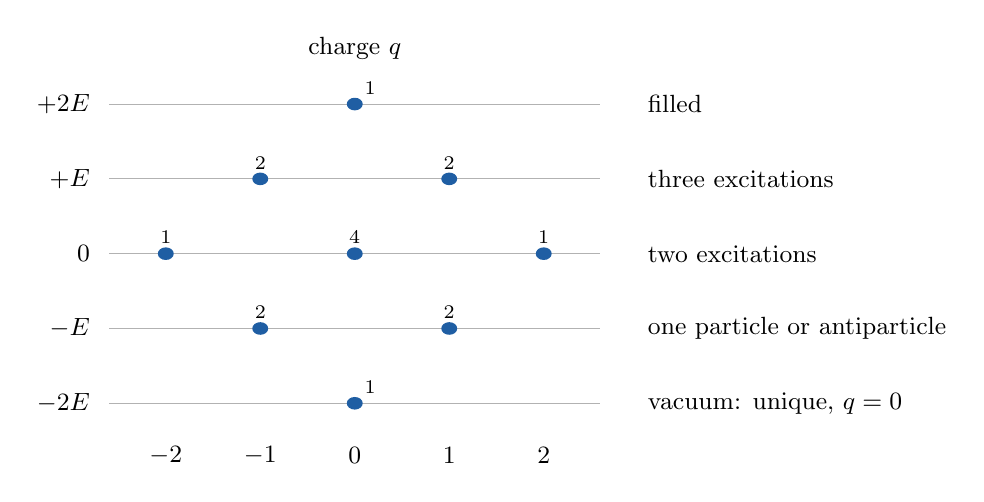
\begin{tikzpicture}[xscale=1.2,yscale=0.95]
\foreach \y/\l in {-2/{-2E},-1/{-E},0/{0},1/{+E},2/{+2E}}{
  \draw[gray!60] (-2.6,\y) -- (2.6,\y);
  \node[left] at (-2.7,\y) {\small $\l$};
}
\node at (0,2.75) {\small charge $q$};
\foreach \q in {-2,-1,0,1,2}{\node at (\q,-2.7) {\small $\q$};}
% ground state
\fill[tcol] (0,-2) circle (2.4pt); \node[above right] at (0,-2) {\scriptsize 1};
% -E level
\fill[tcol] (-1,-1) circle (2.4pt); \fill[tcol] (1,-1) circle (2.4pt);
\node[above] at (-1,-1) {\scriptsize 2}; \node[above] at (1,-1) {\scriptsize 2};
% 0 level
\fill[tcol] (-2,0) circle (2.4pt); \fill[tcol] (2,0) circle (2.4pt); \fill[tcol] (0,0) circle (2.4pt);
\node[above] at (-2,0) {\scriptsize 1}; \node[above] at (2,0) {\scriptsize 1}; \node[above] at (0,0) {\scriptsize 4};
% +E
\fill[tcol] (-1,1) circle (2.4pt); \fill[tcol] (1,1) circle (2.4pt);
\node[above] at (-1,1) {\scriptsize 2}; \node[above] at (1,1) {\scriptsize 2};
% +2E
\fill[tcol] (0,2) circle (2.4pt); \node[above right] at (0,2) {\scriptsize 1};
\node[align=left,anchor=west] at (3.0,-2) {\small vacuum: unique, $q=0$};
\node[align=left,anchor=west] at (3.0,-1) {\small one particle or antiparticle};
\node[align=left,anchor=west] at (3.0,0) {\small two excitations};
\node[align=left,anchor=west] at (3.0,1) {\small three excitations};
\node[align=left,anchor=west] at (3.0,2) {\small filled};
\end{tikzpicture}
\caption{The Fock space of one momentum (\cref{thm:spectra}). Each dot is a joint eigenspace of energy and charge, labelled by its
dimension. The multiplicities $1,4,6,4,1$ are those of four fermionic modes: two particle and two antiparticle states of one Dirac
flavour, read off rather than inferred.}
\label{fig:fock}
\end{figure}

The multiplicities $1,4,6,4,1$ are the binomial coefficients of a four-mode Fock space, as a single Dirac flavour with two particle and
two antiparticle states must give. The ground state at $-2E$ is the zero-point energy $-\tfrac12\sum E$ of the four modes; summed over
momenta it is the familiar fermion term of the one-loop effective potential. A projector built from $\rho(JH)^2$ could not have
produced the table: squaring loses the sign of the energy and conflates the vacuum with the filled state.

\begin{proposition}[Conjugation on states]
\label{prop:Cstates}
$C\in SO(8)$ lifts to $\mathrm{Spin}(8)$ as a product of four integral reflections. The lift is unitary on $\mathcal F$, anticommutes with
$Q$ and carries $H(p)$ to $H(-p)$, so $\langle\psi|Q|\psi\rangle=0$ for every $C$-eigenstate. The stronger statement $Q|\psi\rangle=0$ is
false: the $+1$ eigenspace of $C$ has real dimension eight and $Q$ annihilates only a three-dimensional part of it.
\end{proposition}

\begin{remark}[Many-body chirality is a group lift]
$\rho$ is a homomorphism of Lie algebras only, so the product $\rho(J)\rho(\Omega)$, of rank eight, is not a $\mathrm{Spin}(8)$ element and
is not the chirality of the module. The correct object is $\Gamma_{\mathcal F}=\exp[\tfrac\pi2(\rho(J)+\rho(\Omega))]$, an involution of
$\mathcal F$ whose eigenvalue on a joint eigenvector is $i^{q_J+q_\Omega}$; the sectors are labelled by the parity of
$\tfrac12(q_J+q_\Omega)$.
\end{remark}

\part{The tower and its matter}
\section{The tower: centralisers, nesting, and carriers}
\label{sec:tower}

Climbing the tower adds six directions per rung and leaves the local structure of each factor unchanged. The interior four-plane
stays in the first factor; the question is what the added directions do to the internal symmetry.

\begin{theorem}[Internal centraliser]
\label{thm:centraliser}
In $\Cl(3n,3n)$ the bivectors commuting with the interior Lorentz action form
\[
\gint^{(n)}\cong\so{3n-1,3n-3},\qquad \dim\gint^{(n)}=\tfrac12(6n-4)(6n-5).
\]
\end{theorem}

\begin{proof}
By \eqref{eq:bladecomm} a bivector sharing exactly one index with an interior bivector anticommutes with it, and one sharing none
or two commutes. A bivector commuting with all six interior bivectors therefore has either both indices in $E$, which gives
$\lint$ itself and is excluded by commutation with the boosts, or both indices in the Lorentz complement
\[
W_n=\langle e^{(1)}_2,e^{(1)}_3\rangle\oplus\bigoplus_{k=2}^n\langle e^{(k)}_1,\dots,e^{(k)}_6\rangle ,
\]
which has $3n-1$ positive and $3n-3$ negative directions. All bivectors of $W_n$ commute with $\lint$, and they span $\so{W_n}$.
\end{proof}

\begin{corollary}[The photon at one constituent]
\label{cor:photon1}
At $n=1$, $W_1=U$ and $\gint^{(1)}=\R J$. The electromagnetic $\uu1$ is not a symmetry of the interior structure but the
symmetry, by exhaustion. In agreement with \cref{prop:gauge1}, no other charge direction gauges at $n=1$.
\end{corollary}

\begin{proposition}[One frame, and nesting]
\label{prop:frame}
The interior four-plane lies in the first tensor factor, so the six interior bivectors have the same index sets at every rung and
identical structure constants. The tower is one Lorentz frame with an increasing family of modules over it. Moreover
$W_1\subset W_2\subset\cdots$, hence
\[
\gint^{(1)}\subset\gint^{(2)}\subset\gint^{(3)}\subset\cdots,\qquad \dim=1,\ 28,\ 91,\ 190,\ 325,\dots,
\]
with direct limit $\so{\infty,\infty}$. A connection valued at one rung is a connection at every higher rung with no matching
condition. The inclusion runs in the wrong direction to justify a truncation to low rungs, which would be a separate postulate.
\end{proposition}

A gauge algebra has to be compact, and every compact subalgebra of a reductive real Lie algebra is conjugate into a maximal compact
one \cite{Knapp,Helgason}, here $\so{3n-1}\oplus\so{3n-3}$. Since $\su2$ needs a faithful real representation of dimension at least
three and $\su3$ one of dimension at least six \cite{GoodmanWallach}, the rungs can be sorted by what they can carry.

\begin{theorem}[Carrier census]
\label{thm:census}
\[
\begin{array}{c|l|l|r|r|c|c|c}
\toprule
n & \gint^{(n)} & \text{maximal compact} & \dim & \text{rank} & \uu1\ \text{alone} & \su2 & \su3\\
\midrule
1 & \so{2,0} & \so2 & 1 & 1 & \text{yes} & \text{no} & \text{no}\\
2 & \so{5,3} & \so5\oplus\so3 & 13 & 3 & \text{no} & \text{yes} & \text{no}\\
3 & \so{8,6} & \so8\oplus\so6 & 43 & 7 & \text{no} & \text{yes} & \text{yes}\\
4 & \so{11,9} & \so{11}\oplus\so9 & 91 & 9 & \text{no} & \text{yes} & \text{yes}\\
\bottomrule
\end{array}
\]
At $n=2$ the projection of a simple $\su3$ to $\so3$ must vanish and $\so5$ has no proper subalgebra of dimension above six; at
$n=3$ colour enters through $\su3\subset\su4\cong\so6$.
\end{theorem}

\begin{lemma}[Rank obstruction]
\label{lem:rank}
$\rank(\su3\oplus\su2\oplus\uu1)=4$, while the maximal compact subalgebras above have ranks $1,3,7,9$. The full Standard-Model
algebra therefore embeds at no rung $n\le2$. At $n=2$ the maximal compact subalgebra has dimension $13\ge12$, so dimension counting
alone would admit it, and rank is the sharp invariant.
\end{lemma}

\begin{figure}[t]
\centering
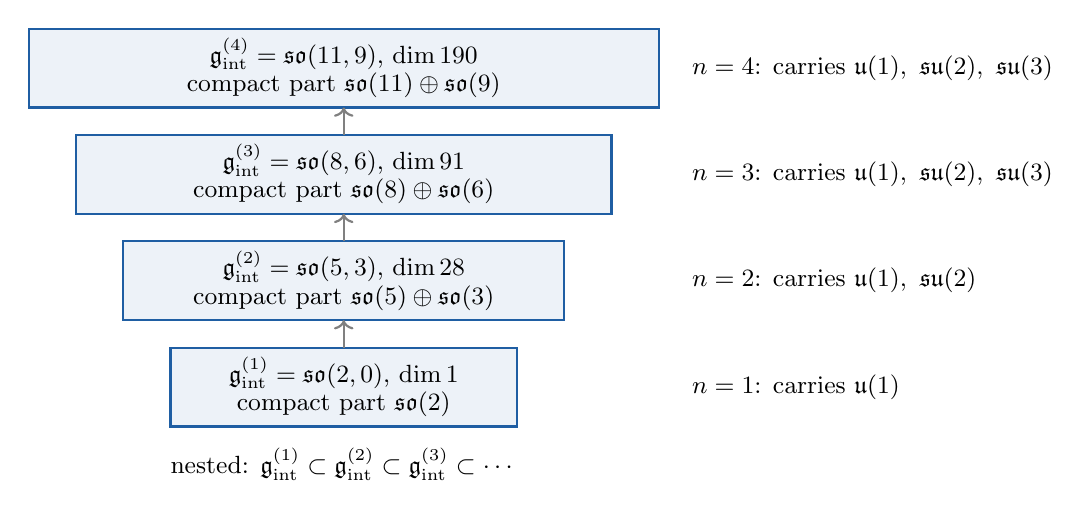
\begin{tikzpicture}[scale=1.0]
\foreach \n/\alg/\dimc/\cmp/\cr in {1/{\so{2,0}}/{1}/{\so2}/{\uu1},2/{\so{5,3}}/{28}/{\so5\oplus\so3}/{\uu1,\ \su2},3/{\so{8,6}}/{91}/{\so8\oplus\so6}/{\uu1,\ \su2,\ \su3},4/{\so{11,9}}/{190}/{\so{11}\oplus\so9}/{\uu1,\ \su2,\ \su3}}{
  \pgfmathsetmacro{\y}{1.35*(\n-1)}
  \pgfmathsetmacro{\w}{1.6+0.6*\n}
  \fill[tcol!8] (-\w,\y) rectangle (\w,\y+1.0);
  \draw[tcol,thick] (-\w,\y) rectangle (\w,\y+1.0);
  \node at (0,\y+0.68) {\small $\gint^{(\n)}=\alg$, $\dim\dimc$};
  \node at (0,\y+0.28) {\small compact part $\cmp$};
  \node[anchor=west] at (4.3,\y+0.5) {\small $n=\n$: carries $\cr$};
}
\foreach \n in {1,2,3}{\pgfmathsetmacro{\y}{1.35*\n-0.35}\draw[->,thick,gray] (0,\y-0.0) -- (0,\y+0.35);}
\node[anchor=north] at (0,-0.15) {\small nested: $\gint^{(1)}\subset\gint^{(2)}\subset\gint^{(3)}\subset\cdots$};
\end{tikzpicture}
\caption{The tower of internal centralisers (\cref{thm:centraliser,thm:census}). Each rung contains the previous one; the compact part
decides which gauge factors can be carried. The electromagnetic $\uu1$ is the whole centraliser only at the first rung, the one rung
with no room for a nonabelian factor.}
\label{fig:tower}
\end{figure}

\begin{corollary}[The tower's trade-off]
\label{cor:tradeoff}
The $\uu1$ is the whole internal centraliser only at $n=1$, the one rung with no room for either nonabelian carrier. Inside
$\gint^{(n)}$ the centraliser of the embedded one-rung charge $e^{(1)}_2e^{(1)}_3$ has dimensions $1,16,67,154,277$ for $n=1,\dots,5$,
since by \eqref{eq:bladecomm} exactly $12(n-1)$ internal bivectors fail to commute with it. From $n=2$ onwards the photon is one
direction in a space that grows without bound; its uniqueness is lost to no dynamical process, only to the arrival of room.
\end{corollary}

At $n\ge2$ the embedded one-rung charge $e^{(1)}_2e^{(1)}_3$ must not be confused with the complex structure $J=\wI$ of
\cref{thm:i}, which commutes with every internal bivector and has all of $\gint^{(n)}$ as centraliser; they agree only at $n=1$.

\begin{remark}[The gaugeable fraction does not improve]
Of the $\binom{6n}2=3n(6n-1)$ bivectors of $\Cl(3n,3n)$, $2\binom{3n}2=3n(3n-1)$ pair directions of the same sign: the fractions
$6/15$, $30/66$, $72/153$ rise only to $1/2$. Climbing adds boosts at essentially the rate at which it adds rotations. The census
permits the chain $\uu1\subset\uu1\oplus\su2\subset\uu1\oplus\su2\oplus\su3$ at $n=1,2,3$; it permits it, and nothing selects those
subalgebras among others of the same rank.
\end{remark}

\section{Chirality, projectors, and colour}
\label{sec:projectors}

\subsection{Unprojected matter is vector-like}

With $i=J$ and $\gamma_5=\Gamma$ as in \cref{thm:i}, consider the part of the Lorentz commutant that preserves chirality. It splits
into a \emph{vector class} $\Cl^0(W)$, the even subalgebra of the internal directions, whose elements commute with the interior gamma
matrices, and an \emph{axial class} $\Omega\,\Cl^0(W)$, whose elements anticommute with them.

\begin{proposition}[Unprojected matter is vector-like]
\label{prop:vectorlike}
Every grade-two internal algebra lies in the vector class. For a gauge algebra in the vector class, $\gamma_\mu$ is an invertible,
complex-linear, gauge-equivariant map between the two chirality sectors, so the unprojected matter is vector-like at every rung.
\end{proposition}

\begin{proposition}
\label{prop:axialtriple}
The two classes form a symmetric pair, $[\mathrm a,\mathrm a]\subseteq\mathrm v$, so the axial class is a Lie triple system and no
nonabelian gauge algebra lies entirely inside it.
\end{proposition}

This does not exclude generators with both parts. If $[\Gamma,t_a]=0$ and $P_L=\tfrac12(\id-\Gamma)$, then
\[
[P_Lt_a,P_Lt_b]=P_L^2[t_a,t_b]=\epsilon_{abc}P_Lt_c ,
\]
a nonabelian algebra, half vector and half axial. Such \emph{dressing} is available to nonabelian carriers exactly as to abelian ones;
only the purely axial summand is excluded. For scalar dressings $f(\Gamma)t_a$ with $f=a+b\Gamma$ and unchanged structure constants,
closure forces $f^2=f$, that is $a^2+b^2=a$ and $2ab=b$, so $f\in\{0,\id,P_L,P_R\}$.

\subsection{A family of projectors at three constituents}

To obtain chiral matter one must project. At $n=3$ write $J^{(k)}=e^{(k)}_2e^{(k)}_3$ for the surplus bivector and
$\omega^{(k)}=e^{(k)}_1\cdots e^{(k)}_6$ for the volume of constituent $k$, and $K^{(3)}_{14}=e^{(3)}_1e^{(3)}_4$ for the pole bivector
joining the first temporal and the first spatial direction of constituent three. The three operators
\[
X_1=J^{(1)}J^{(2)},\qquad X_2=\omega^{(3)},\qquad X_3=\omega^{(1)}K^{(3)}_{14}
\]
are commuting symmetric traceless involutions, and they generate the orthogonal projectors $P_1=\tfrac12(\id+X_1)$ of rank $256$,
$P_{ij}=\tfrac14(\id+X_i)(\id+X_j)$ of rank $128$, and $\Pfam=\tfrac18\prod_i(\id+X_i)$ of rank $64$.

\begin{definition}[Ambient and faithful algebra]
\label{def:keff}
For an orthogonal projector $P$ commuting with the Lorentz action let $\mathfrak g_{\rm phys}(P)$ be the internal bivectors commuting
with $P$, $\mathfrak k(P)$ its compact part (the $+1$ eigenspace of $\theta(X)=-X^{\!\top}$), and
\[
\keff(P)=\mathfrak k(P)\big/\{X\in\mathfrak k(P):XP=0\}.
\]
\end{definition}

The quotient is not a technicality: an element can preserve the block and annihilate every state in it.

\begin{example}[An annihilator]
\label{ex:annihilator}
With $X_1=J^{(1)}J^{(2)}$, $(J^{(1)})^2=(J^{(2)})^2=-\id$ and $[J^{(1)},J^{(2)}]=0$,
\[
(J^{(1)}+J^{(2)})(\id+X_1)=J^{(1)}+J^{(2)}+(J^{(1)})^2J^{(2)}+J^{(2)}J^{(1)}J^{(2)}=J^{(1)}+J^{(2)}-J^{(2)}-J^{(1)}=0 .
\]
So $J^{(1)}+J^{(2)}$ is a compact element of $\mathfrak k(\Pfam)$ that annihilates the block of $\Pfam$, although it does not annihilate the
block of $P_{23}$. A table of gauge algebras that omits the quotient overcounts, here by three dimensions.
\end{example}

\begin{theorem}[The projector family]
\label{thm:table}
Computed on the $512$-dimensional module as the exact nullspace of $X\mapsto[X,P]$ over the $\binom{14}2=91$ internal bivectors, with
$\keff$ decomposed on the image:
\begin{center}
\begin{tabular}{@{}lrrrrrlc@{}}
\toprule
$P$ & rank & $\dim\mathfrak g_{\rm phys}$ & $\dim\mathfrak k$ & $\dim\mathfrak p$ & $\dim\ker$ & $\keff$ & axial\\
\midrule
$\Pfam$ & $64$ & $17$ & $9$ & $8$ & $3$ & $\uu1^3\oplus\su2$ & yes\\
$P_{23}$ & $128$ & $23$ & $9$ & $14$ & $0$ & $\uu1^3\oplus\su2\oplus\su2$ & yes\\
$P_{13}$ & $128$ & $33$ & $17$ & $16$ & $3$ & $\uu1\oplus\su2\oplus\so5$ & yes\\
$P_{12}$ & $128$ & $27$ & $15$ & $12$ & $3$ & $\su2^{\oplus4}$ & no\\
$P_1$ & $256$ & $51$ & $27$ & $24$ & $3$ & $\so6\oplus\su2^{\oplus3}$ & no\\
\bottomrule
\end{tabular}
\end{center}
Here a projector is axial when $P\gamma^\mu P=0$. Factors are identified by dimension and rank: $(3,1)=\su2$, $(10,2)=\so5\cong\spp2$,
$(15,3)=\so6\cong\su4$; a six-dimensional semisimple compact factor is necessarily $\su2\oplus\su2$. The centres have dimensions
$3,3,1,0,0$ and the derived algebras $3,6,13,12,24$.
\end{theorem}

\begin{corollary}[No colour on the axial members]
\label{cor:nocolour}
The largest simple factor among the rank-$64$ and rank-$128$ blocks is $\so5$, every proper subalgebra of which has dimension at most
six. Since $\su3$ is simple of dimension eight, it embeds in none of them. Dimension eight is necessary and not sufficient: $P_{13}$
carries an $\so5$ of dimension ten and still contains no $\su3$, so the test is an embedding test.
\end{corollary}

\subsection{Colour at rank 256}

\begin{theorem}[Colour on $P_1$]
\label{thm:su3}
Let $f_1,\dots,f_6$ be the six spatial directions of the second and third constituents. The fifteen bivectors $f_af_b$ square to
$-\id$, are antisymmetric and close on $\so6$; each commutes with $X_1$, because the index sets are disjoint and $2\cdot4$ is even in
\eqref{eq:bladecomm}, so all fifteen preserve $P_1$ and act faithfully on its image. Let $\Omega_6=f_1f_4+f_2f_5+f_3f_6$ generate the pairing
$f_k\mapsto f_{k+3}$. Its centraliser in $\so6$ has dimension nine and is $\uu3$; the derived algebra has dimension eight and rank two, is
compact, closed and simple, hence $\su3$, and its eight generators act faithfully on the block.
\end{theorem}

\begin{theorem}[$P_1$ is vector-like undressed]
\label{thm:p1}
$X_1$ is a product of four generators, none of them interior, so $|I||J|-|I\cap J|=4$ is even for every interior generator and
$[X_1,\gamma_\mu]=0$. Hence $P_1$ is not axial and its matter is vector-like by \cref{prop:vectorlike}.
\end{theorem}

The obstruction is to the undressed action only.

\begin{theorem}[Colour with a chiral doublet on $P_1$]
\label{thm:p1chiral}
Keep the colour generators in the six negative directions of factors two and three, and in the three positive directions of factor
three set
\[
t_1=\tfrac12e^{(3)}_1e^{(3)}_2,\qquad t_2=\tfrac12e^{(3)}_1e^{(3)}_3,\qquad t_3=-\tfrac12e^{(3)}_2e^{(3)}_3 .
\]
With $P_{1,L}=P_1\tfrac12(\id-\Gamma)$ and $L_i=P_{1,L}t_i$,
\[
[L_i,L_j]=\epsilon_{ij}{}^kL_k,\qquad [C_A,L_i]=0,\qquad -\sum_iL_i^2=\tfrac34P_{1,L},\qquad L_iP_{1,R}=0
\]
for every colour generator $C_A$. Vector colour and a commuting, purely left-handed doublet action therefore coexist on $P_1$.
\end{theorem}

\begin{proof}
The $t_i$ are half time--time bivectors of factor three, so each squares to $-\tfrac14\id$ and they close on $\su2$. The colour generators
carry only negative indices of factors two and three, disjoint from $\{e^{(3)}_1,e^{(3)}_2,e^{(3)}_3\}$, and two even blades with disjoint
supports commute. $P_{1,L}$ is an idempotent of rank $128$ commuting with each $t_i$, so $L_i=P_{1,L}t_i$ inherits the bracket and
$-\sum L_i^2=P_{1,L}(-\sum t_i^2)=\tfrac34P_{1,L}$, the Casimir of a doublet. $P_{1,L}P_{1,R}=0$ gives the last identity.
\end{proof}

Ordering the family by $\dim\keff$ and recording whether the projector is axial,
\[
\Pfam\,(6)\ \text{axial},\quad P_{23}\,(9)\ \text{axial},\quad P_{12}\,(12)\ \text{not},\quad P_{13}\,(14)\ \text{axial},\quad P_1\,(24)\ \text{not},
\]
the two orderings are not reverses of one another, and what survives is a statement about these five projectors only: no axial one
carries $\su3$ in its effective bivector algebra, and $\su3$ appears on exactly one of them, the vector-like $P_1$. The pattern is
not a law of the arena. The next section exhibits a projector outside the family on which colour and chirality coexist.

\section{A chiral Pati--Salam block}
\label{sec:pstar}

The five projectors of \cref{sec:projectors} are one family among many. Enlarging the class to all commuting symmetric blade
involutions produces a projector on which colour and chirality coexist. The idea is to correlate spacetime chirality with an
\emph{internal} four-dimensional chirality, and to constrain the colour \emph{volume} rather than any colour direction.

\subsection{Construction}

At three constituents take the interior gamma matrices $\gamma^\mu=(e^{(1)}_1,e^{(1)}_4,e^{(1)}_5,e^{(1)}_6)$ and split the remaining
fourteen directions into three groups:
\begin{center}
\begin{tabular}{@{}llcc@{}}
\toprule
group & directions & signs & generators $E_A$\\
\midrule
weak $W$ & $e^{(2)}_1,\ e^{(3)}_1,\ e^{(3)}_2,\ e^{(3)}_3$ & $++++$ & $7,13,14,15$\\
colour $C$ & $e^{(2)}_4,e^{(2)}_5,e^{(2)}_6,\ e^{(3)}_4,e^{(3)}_5,e^{(3)}_6$ & $------$ & $10,11,12,16,17,18$\\
auxiliary $A$ & $e^{(1)}_2,e^{(1)}_3,\ e^{(2)}_2,e^{(2)}_3$ & $++++$ & $2,3,8,9$\\
\bottomrule
\end{tabular}
\end{center}
With $J=\wI$ the ordered product of the fourteen internal generators and $\Gamma=J\gamma^0\gamma^1\gamma^2\gamma^3$, define the three
volumes
\[
\chi_W=e^{(2)}_1e^{(3)}_1e^{(3)}_2e^{(3)}_3,\qquad
\chi_C=e^{(2)}_4e^{(2)}_5e^{(2)}_6e^{(3)}_4e^{(3)}_5e^{(3)}_6,\qquad
q_A=e^{(1)}_2e^{(1)}_3 .
\]

\begin{figure}[t]
\centering
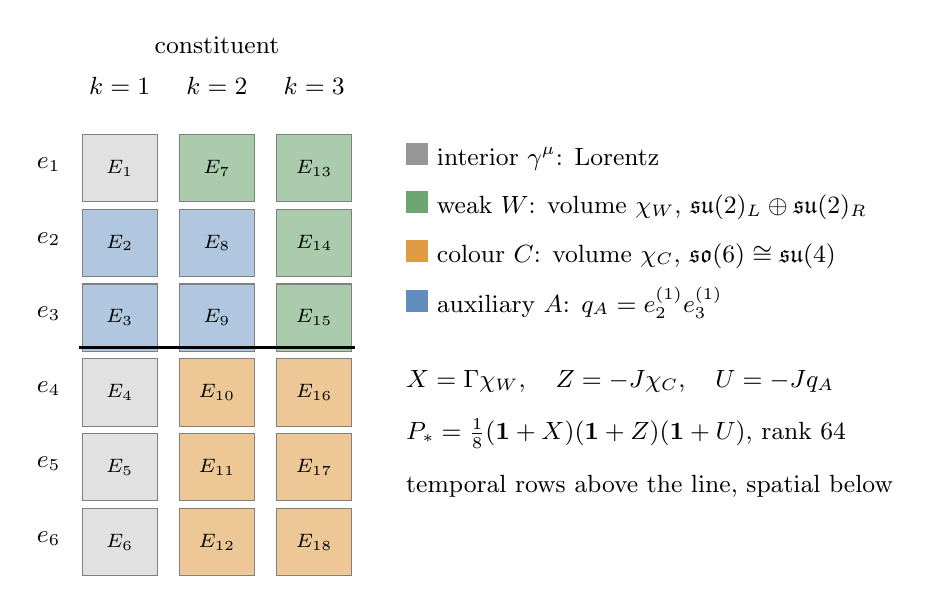
\begin{tikzpicture}[scale=0.95]
\foreach \k in {1,2,3}{\node at (1.3*\k,6.55) {\small $k=\k$};}
\node[anchor=south] at (2.6,6.85) {\small constituent};
\foreach \a in {1,...,6}{\node at (0.35,6.5-\a) {\small $e_{\a}$};}
% colour code: interior = gray, W = gcol, C = ocol, A = tcol
\def\pscell#1#2#3{\fill[#3] (1.3*#1-0.5,6.0-#2) rectangle (1.3*#1+0.5,6.0-#2+0.9);\draw[gray] (1.3*#1-0.5,6.0-#2) rectangle (1.3*#1+0.5,6.0-#2+0.9);}
\pscell{1}{1}{lgray}\pscell{1}{4}{lgray}\pscell{1}{5}{lgray}\pscell{1}{6}{lgray}
\pscell{1}{2}{tcol!35}\pscell{1}{3}{tcol!35}
\pscell{2}{1}{gcol!40}\pscell{2}{2}{tcol!35}\pscell{2}{3}{tcol!35}
\pscell{2}{4}{ocol!45}\pscell{2}{5}{ocol!45}\pscell{2}{6}{ocol!45}
\pscell{3}{1}{gcol!40}\pscell{3}{2}{gcol!40}\pscell{3}{3}{gcol!40}
\pscell{3}{4}{ocol!45}\pscell{3}{5}{ocol!45}\pscell{3}{6}{ocol!45}
\foreach \k in {1,2,3}{\foreach \a in {1,...,6}{\pgfmathtruncatemacro{\A}{6*(\k-1)+\a}\node at (1.3*\k,6.45-\a) {\scriptsize $E_{\A}$};}}
\draw[thick] (0.75,3.05) -- (4.45,3.05);
\node[anchor=west,align=left] at (5.0,5.6) {\small \textcolor{mgray}{\rule{8pt}{8pt}} interior $\gamma^\mu$: Lorentz};
\node[anchor=west,align=left] at (5.0,4.95) {\small \textcolor{gcol!70}{\rule{8pt}{8pt}} weak $W$: volume $\chi_W$, $\su2_L\oplus\su2_R$};
\node[anchor=west,align=left] at (5.0,4.3) {\small \textcolor{ocol!80}{\rule{8pt}{8pt}} colour $C$: volume $\chi_C$, $\so6\cong\su4$};
\node[anchor=west,align=left] at (5.0,3.65) {\small \textcolor{tcol!70}{\rule{8pt}{8pt}} auxiliary $A$: $q_A=e^{(1)}_2e^{(1)}_3$};
\node[anchor=west,align=left] at (5.0,2.6) {\small $X=\Gamma\chi_W,\quad Z=-J\chi_C,\quad U=-Jq_A$};
\node[anchor=west,align=left] at (5.0,1.9) {\small $P_*=\tfrac18(\id+X)(\id+Z)(\id+U)$, rank $64$};
\node[anchor=west,align=left] at (5.0,1.2) {\small temporal rows above the line, spatial below};
\end{tikzpicture}
\caption{The eighteen generators of $\Cl(9,9)$ arranged by constituent, and the grouping that defines the Pati--Salam block. The
interior four-plane carries the Lorentz action; the weak, colour and auxiliary groups enter $P_*$ only through their volumes, which
is why every rotation inside each group survives the projection (\cref{thm:PS,thm:PSalg}).}
\label{fig:pstar}
\end{figure}

\begin{theorem}[A chiral projector carrying colour]
\label{thm:PS}
$X=\Gamma\chi_W$, $Z=-J\chi_C$ and $U=-Jq_A$ are commuting symmetric traceless involutions, and all seven nonidentity products $X$, $Z$,
$U$, $XZ$, $XU$, $ZU$, $XZU$ are traceless. Hence
\begin{equation}
\label{eq:Pstar}
P_*=\tfrac18(\id+\Gamma\chi_W)(\id-J\chi_C)(\id-Jq_A)
\end{equation}
is an orthogonal projector with $\Tr P_*=512/8=64$. It satisfies $[P_*,\Sigma^{\mu\nu}]=[P_*,J]=0$ for the six Lorentz generators
$\Sigma^{\mu\nu}=\tfrac12\gamma^\mu\gamma^\nu$, and $P_*\gamma^\mu P_*=0$, so it is axial; its two Weyl blocks have real rank $32$ each, and
$\chi_WP_*=\Gamma P_*$.
\end{theorem}

Rank is not automatic from the three factors being individually traceless; it is the products that decide, and here all of them are
traceless. The statement $\chi_WP_*=\Gamma P_*$ is the correlation of spacetime chirality with the internal chirality of the weak
directions.

\subsection{The effective algebra}

\begin{theorem}[The effective algebra and its Pati--Salam part]
\label{thm:PSalg}
All fifteen colour bivectors $e_ae_b$, $a,b\in C$, commute with $X$, $Z$ and $U$, so the whole compact $\so6_C\cong\su4_C$ survives
and acts faithfully on the block; the colour volume $\chi_C$ is invariant under those rotations, so constraining it costs no colour
generator. With $w_1,\dots,w_4$ the weak directions, $\tau_i=-\tfrac12w_jw_k$ for cyclic $(i,j,k)$, $t^{L,R}_i=\tfrac12(\id\mp\chi_W)\tau_i$
and $T^{L,R}_i=P_*t^{L,R}_i$,
\[
[T^L_i,T^L_j]=\epsilon_{ijk}T^L_k,\qquad T^L_iP_R=0,\qquad -\sum_i(T^L_i)^2=\tfrac34P_L,
\]
and the mirror identities hold on the right. The $t^{L,R}_i$ are genuine bivectors, for example $t^L_3=-\tfrac14(w_1w_2+w_3w_4)$.
The full effective compact bivector algebra is
\[
\keff(P_*)=\su4\oplus\su2_L\oplus\su2_R\oplus\uu1^2,
\]
of dimension $23$, entirely compact, with a derived algebra of dimension $21$ and a two-dimensional centre. All $21$ simple generators
preserve the kinetic kernels $K^\mu=P_*\gamma^0\gamma^\mu P_*$, and $K^0=P_*$.
\end{theorem}

\begin{proof}
Each colour bivector has even overlap with each of the three involution masks, so all fifteen commute with $X,Z,U$ and descend
faithfully. For the weak part, $\chi_W^2=\id$ and $[\chi_W,\tau_i]=0$ make $\tfrac12(\id\mp\chi_W)$ idempotents commuting with the
$\tau_i$; the $\tau_i$ close on $\su2$ with $\tau_i^2=-\tfrac14\id$, so $-\sum_i(T^L_i)^2=\tfrac34P_L$, and $\chi_WP_*=\Gamma P_*$ places the
two ideals on opposite chiralities. The dimension $23$ is the full solution of $[B,P_*]=0$ over the $91$-dimensional space of internal
bivectors: the nullspace is $23$-dimensional, entirely compact, has trivial annihilator on the block, and has a derived algebra of
dimension $21$.
\end{proof}

\begin{corollary}[One Pati--Salam family]
\label{cor:PSfamily}
The colour volume is not an involution: $\chi_C$ is a grade-six blade on six negative directions, so $\chi_C^2=-\id$. The
involution is
\[
\Gamma_C:=J\chi_C,\qquad \Gamma_C^2=\id,\qquad \Gamma_CP_*=-P_*,\quad\text{equivalently}\quad \chi_CP_*=JP_*.
\]
On the module with $J=+i$ each Weyl block then carries exactly four $\su4$ weights, all of colour chirality $\Gamma_C=-1$, each with
multiplicity $4=2\times2$, a weak doublet times a Weyl spinor, and the two blocks carry the same colour weights. The content is
\[
(\mathbf4,\mathbf2,\mathbf1)_L\oplus(\mathbf4,\mathbf1,\mathbf2)_R ,
\]
one Pati--Salam family including a right-handed neutrino \cite{PatiSalam}. Which of the two conjugate four-dimensional representations
is called $\mathbf4$ is a convention.
\end{corollary}

\subsection{Charges}

The compact algebra is realised by skew operators; charges are the corresponding symmetric operators $\hat t=-Jt$. On the block the
centre of $\keff(P_*)$ is spanned by the skew operators $JP_*$ and $J\Gamma P_*$, whose charges are $P_*$ and $\Gamma P_*$. Concretely
$q_A|_{V_*}=J$ and $E_8E_9|_{V_*}=J\Gamma$ on the image $V_*=\operatorname{im}P_*$.

\begin{proposition}[Colour intertwiner, $\BmL$, and the charge table]
\label{prop:PSledger}
$R=P_*\gamma^0e^{(2)}_1e^{(2)}_2$ satisfies $R^2=-P_*$, exchanges the two Weyl blocks and commutes with every colour generator, so the
colour representations of the two chiralities are equivalent and the content is $(\mathbf4,\mathbf2,\mathbf1)_L\oplus(\mathbf4,\mathbf1,
\mathbf2)_R$ rather than a $\mathbf4/\bar{\mathbf4}$ pairing. With
\[
H=-\bigl(e^{(2)}_4e^{(3)}_4+e^{(2)}_5e^{(3)}_5+e^{(2)}_6e^{(3)}_6\bigr),\qquad Q_c=-JH,
\]
the derived centraliser of $H$ inside colour $\so6$ is $\su3$, and $(Q_c-\id)(Q_c+3\id)P_*=0$: $Q_c$ has eigenvalues $+1$ and $-3$ on
the block, with real multiplicities $48$ and $16$, the triplet and the singlet. Setting $\BmL=Q_c/3$ and using the weak charges
$-JT^3_{L,R}$,
\[
Y=-J\,T^3_R+\tfrac12(\BmL),\qquad Q=-J\,T^3_L+Y ,
\]
gives one family:
\begin{center}
\begin{tabular}{@{}lccr@{}}
\toprule
field & $SU(3)\times SU(2)_L$ & $Y$ & internal Weyl components\\
\midrule
$Q_L$ & $(\mathbf3,\mathbf2)$ & $\tfrac16$ & $6$\\
$L_L$ & $(\mathbf1,\mathbf2)$ & $-\tfrac12$ & $2$\\
$u_R$ & $(\mathbf3,\mathbf1)$ & $\tfrac23$ & $3$\\
$d_R$ & $(\mathbf3,\mathbf1)$ & $-\tfrac13$ & $3$\\
$e_R$ & $(\mathbf1,\mathbf1)$ & $-1$ & $1$\\
$\nu_R$ & $(\mathbf1,\mathbf1)$ & $0$ & $1$\\
\bottomrule
\end{tabular}
\end{center}
Four real spinor coordinates make one internal Weyl component, so rank $64$ is sixteen internal Weyl components, eight left and eight
right, and not sixty-four particles.
\end{proposition}

The $\su3$ embedding, the right-handed Cartan direction and the hypercharge combination are chosen; what is established is their
mutual compatibility. In the complex structure $J$ every one of the sixteen Weyl fermions has charge one: $J$ is fermion number,
$F=3B+L$, and the baryon number appears as $4B=F+(\BmL)$.

\begin{proposition}[The two central factors cannot be gauged]
\label{prop:PSanom}
For a central charge $a+b\Gamma$, corresponding to the skew element $aJ+bJ\Gamma$, the anomaly coefficients on the block, per Weyl
fermion with every field written left-handed, are
\[
\begin{gathered}
SU(2)_L^2:\ 2(a-b),\qquad SU(2)_R^2:\ -2(a+b),\qquad SU(4)^2:\ -2b,\\
\text{cubic}:\ -16(3a^2b+b^3),\qquad \text{gravitational}:\ -16b ,
\end{gathered}
\]
and the mixed anomalies with two central and one Pati--Salam generator vanish. All vanish only for $a=b=0$. The Pati--Salam algebra itself
is anomaly free on the block: the $SU(4)^3$ anomaly cancels between two fundamentals and two antifundamentals in the all-left convention,
and each weak $SU(2)$ sees four doublets, so the global anomaly is absent \cite{Witten82}. Hence, with the block as the matter content,
$\su4\oplus\su2_L\oplus\su2_R$ is the largest anomaly-free gauge algebra containing Pati--Salam, and the two central directions remain
global symmetries.
\end{proposition}

The obstruction is stated for this matter content; additional matter or another cancellation mechanism is not excluded. The two central
symmetries are fermion number $J$, anomalous only through $SU(2)_L$ and $SU(2)_R$ and hence exact in perturbation theory and violated by
their instantons \cite{tHooft76}, and the chiral charge $J\Gamma$.

\begin{proposition}[Two rank-64 projectors, two orbits]
\label{prop:orbits}
Under the compact group of the connection sector, whose Lie algebra is the maximal compact $\so8\oplus\so6$ of dimension $43$, the orbit
through $\Pfam$ has dimension $43-9=34$ and the orbit through $P_*$ has dimension $43-23=20$. Equal rank does not put two projectors on
one orbit.
\end{proposition}

\begin{remark}[What the construction settles]
\label{rem:PSsettles}
It settles an existence question: colour on a chiral block is not obstructed, and no counting argument based on the five-projector family
can be a theorem. It does not select $P_*$; it does not derive the hypercharge embedding, which is compatible with anomaly cancellation but
chosen; it gives one family and not three; and by \cref{cor:nopredict} exhibiting a known representation content is a consistency result,
not evidence. One further fact will matter in \cref{sec:matter}: $\gamma^0$ commutes with all $91$ internal bivectors and with $J$ and the
rotations, and anticommutes with $\Gamma$ and the boosts. It maps $V_*$ onto an orthogonal rank-$64$ subspace on which the same internal
algebra acts with $\Gamma$ reversed. The chirality of the block is put in by the choice of $P_*$.
\end{remark}

\section{Charges and anomalies}
\label{sec:charges}

The weak and colour algebras of a block are fixed by the projector; the abelian charges are not. This section asks how much the
algebra says about them, first inside the arena and then in a layer that uses nothing from the arena at all.

\subsection{A pairing obstruction}
\label{sec:pairing}

The family block of $\Pfam$ carries three abelian charges. The centre of $\keff(\Pfam)$ is spanned by the block images of
$X_a\in\{\tfrac12J^{(1)},\tfrac12J^{(3)},\tfrac12e^{(3)}_5e^{(3)}_6\}$, and their charges $q_a:=-J(2X_a)\Pfam$ are commuting symmetric
involutions of the block, with eigenvalues $\pm1$ and $\Tr q_a=0$. The cubic anomaly of $u=aq_1+bq_2+cq_3$ is the chiral trace
\[
\mathcal A(u^3)=\tfrac14\bigl[\Tr(u^3P_L)-\Tr(u^3P_R)\bigr],\qquad P_{L,R}=\Pfam\tfrac12(\id\mp\Gamma),
\]
per Weyl component, right-handed components entering with conjugated charge when every field is written left-handed. Since
$q_a^2=\Pfam$ and the linear chiral traces vanish, only the mixed term survives:
\[
\mathcal A(u^3)=6abc\,\mathcal A(q_1q_2q_3)=96\,abc ,
\]
while the plain trace $\Tr(u^3)$ vanishes for every $u$ and carries no information about anomalies. The anomaly-free locus is the union
of the three coordinate planes $abc=0$, and on it there is nothing to select.

\begin{theorem}[Conjugate pairing]
\label{thm:pairing}
Let a module carry three commuting involutions $q_a$ with eigenvalues $\pm1$ and $\Tr q_a=0$. For every $u=aq_1+bq_2+cq_3$ with
$abc=0$ the weight multiset of $u$ is symmetric, $\mathrm{mult}(w)=\mathrm{mult}(-w)$.
\end{theorem}

\begin{proof}
Take $c=0$; only the joint multiplicities $M_{s_1s_2}$ of $(q_1,q_2)$ matter. The trace conditions give
$M_{++}+M_{+-}-M_{-+}-M_{--}=0$ and $M_{++}-M_{+-}+M_{-+}-M_{--}=0$; adding and subtracting, $M_{++}=M_{--}$ and $M_{+-}=M_{-+}$. The
weight of $(s_1,s_2)$ is $as_1+bs_2$, and $(s_1,s_2)\mapsto(-s_1,-s_2)$ negates it while preserving multiplicities.
\end{proof}

The proof uses only the three linear traces, with no reference to rank, rung or realisation, so within its hypotheses no
enlargement of the block and no ascent of the tower repairs it. Charge pairing is all that is concluded: calling a full matter
representation vector-like would also require the chirality convention and the other gauge factors. And the hypotheses are not
decorative.

\begin{example}[Vanishing traces do not imply pairing]
\label{ex:multiset}
The multiset $\{(-3)^{\times5},1^{\times10},5^{\times1}\}$ has $\sum q=-15+10+5=0$ and $\sum q^3=-135+10+125=0$, yet it is not symmetric under
$q\mapsto-q$. It is realised by three commuting involutions with joint signs and multiplicities $(+,+,+){:}\,1$, $(-,-,+){:}\,10$,
$(+,-,-){:}\,5$: these have traces $(\Tr q_1,\Tr q_2,\Tr q_3)=(-4,-14,6)$, so the hypotheses of \cref{thm:pairing} fail, while
$Y=q_1+q_2+3q_3$ has spectrum $\{5^{\times1},1^{\times10},(-3)^{\times5}\}$ with $\Tr Y=\Tr Y^3=0$. Leaving the hypotheses therefore need not
violate the gravitational condition, which constrains $\Tr Y$ for the gauged combination and not $\Tr q_a$ for each basis charge
\cite{AlvarezGaumeWitten,Bilal}.
\end{example}

\subsection{Dressing, and a benchmark}
\label{sec:benchmark}

The escape from \cref{thm:pairing} is to leave its hypotheses. On the family block let
\[
t^1=-J\cdot\tfrac12e^{(2)}_5e^{(2)}_6,\qquad t^2=-J\cdot\tfrac12e^{(2)}_6e^{(2)}_4,\qquad t^3=-J\cdot\tfrac12e^{(2)}_4e^{(2)}_5
\]
be the weak charges, whose skew counterparts, the rotations of the spatial directions of constituent two, span the derived $\su2$ of
$\keff(\Pfam)$; let $\varepsilon=\pm1$ be an orientation sign, and put $t^a_{L,R}=P_{L,R}t^a$,
\[
B_0=\frac\varepsilon6\,\Gamma(q_1+q_2+q_3),\qquad Y=B_0+t^3_R,\qquad Q_{\rm em}=t^3_L+Y .
\]
The cell sums $\varepsilon\sum_aq_a$ are $\{-1,-1,-1,3\}$ on the $\Gamma=-1$ half and $\{-3,1,1,1\}$ on the other, which gives
$B_0|_{\Gamma=-1}=\{\tfrac16,\tfrac16,\tfrac16,-\tfrac12\}$ and, after adding $t^3_R=\pm\tfrac12$ on the right-handed cells,
$Y\in\{0,-1,\tfrac23,-\tfrac13\}$ there. Over the sixteen left-handed Weyl components $\Tr Y=\Tr Y^3=\Tr T_3^2Y=0$ with four doublets, so all
four anomaly conditions hold, and $\Tr T_3^2/\Tr Q^2=3/8$. This hypercharge is adopted, not derived.

\begin{proposition}[The escape]
\label{prop:escape}
\Cref{thm:pairing} constrains undressed elements of $\uu1^3$, which lie in the vector class. The charge $B_0$ carries a factor $\Gamma$ and is
axial, not an element of $\uu1^3$, so the cubic-trace formula does not apply to it. Once chirality-dressed endomorphisms are admitted,
which abelian charges can be gauged changes, and no-go results proved in the undressed grade-two setting do not carry across; a well-posed
search must say which Clifford grades are permitted alongside $Y^\dagger=Y$, $[Y,t_{La}]=0$ and $[Y,C_A]=0$.
\end{proposition}

Since $P_L+P_R=\id$, $Q_{\rm em}=t^3+B_0$: the chirality dressing cancels identically in the electric charge when the same axis is used in
both terms and is visible only in the split into $T_3$ and $Y$. The value $3/8$ is arithmetic on a charge table; it becomes $\sin^2\theta_W$
only after a common normalisation of the gauge kinetic terms and a matching scale, neither of which is supplied. Five choices enter the
benchmark: the projector, the dressing, which abelian direction is $Y$, which right-handed axis, and the overall sign.

\subsection{A model-independent layer}
\label{sec:modelindep}

The following uses nothing from the arena. It calibrates how much of the hypercharge problem is generic.

\begin{theorem}[The anomaly variety of one family]
\label{thm:variety}
For one family with $N_c$ colours and a right-handed neutrino, with left-handed hypercharges $q,l$ and right-handed $y_u,y_d,y_\nu,y_e$,
the three linear conditions give $l=-N_cq$, $y_d=2q-y_u$, $y_e=2l-y_\nu$. With $h_q=y_u-q$ and $h_\ell=y_\nu-l$ the cubic condition
factorises,
\[
\mathcal A_{Y^3}=6N_cq\,(h_\ell^2-h_q^2),
\]
using $2q^3-y_u^3-(2q-y_u)^3=-6qh_q^2$. The solution set is the union of three planes: $\Pi_A$ ($h_\ell=h_q$), $\Pi_B$ ($h_\ell=-h_q$) and
$\Pi_C$ ($q=l=0$). On $\Pi_A$ the four Yukawa relations $y_u=q+h$, $y_d=q-h$, $y_\nu=l+h$, $y_e=l-h$ hold, so they are consequences of anomaly
cancellation rather than assumptions; $\Pi_B$ is the image of $\Pi_A$ under the exchange $\nu_R\leftrightarrow e_R$. At $N_c=3$ and
$h=\tfrac12$, $\Pi_A$ is the line $Y=Y_{\rm SM}+\lambda(\BmL)$.
\end{theorem}

Anomaly cancellation does not supply the scalar, its hypercharge, or nonvanishing couplings. Quark Yukawa couplings alone do not exclude
$\Pi_C$ either: at $N_c=3$ the point $(q,l,y_u,y_d,y_\nu,y_e)=(0,0,\tfrac12,-\tfrac12,1,-1)$ with scalar hypercharge $\tfrac12$ cancels all four
anomalies and permits both quark Yukawas, yet $h_q=\tfrac12\neq h_\ell=1$. What excludes it is integrality: with $q=0$ the left-handed quarks
carry $\pm\tfrac12$ and a three-quark singlet has half-integral charge.

\begin{theorem}[Without $\nu_R$ hypercharge is quantised]
\label{thm:nonu}
Deleting $\nu_R$ gives $y_e=2l$ and $\mathcal A_{Y^3}=6N_cq(N_c^2q^2-h_q^2)$, so on the generic branch $h_q=\pm N_cq$ is locked and
hypercharge is fixed up to scale and relabelling: at $N_c=3$, $q=\tfrac16$ gives the Standard-Model values with no residual $\BmL$ direction.
\end{theorem}

This is the classical charge-quantisation result \cite{FootLewVolkas,GengMarshak}. Its bearing here is that the difficulty of selecting
hypercharge on a family block exists because the block carries sixteen Weyl components rather than fifteen: the sterile neutrino is both
the block's virtue and the source of the ambiguity.

\begin{proposition}[Integrality, and what it does not fix]
\label{prop:integrality}
On $\Pi_A$ with $Q_{\rm em}=T^3_L+Y$, the leptons carry $Q_\nu=-\lambda$ and $Q_e=-1-\lambda$, so integrality of the charged lepton forces
$\lambda\in\Z$, and colour triality then gives integral charge to every colour singlet. It does not fix the fractional part of the quark
charges, since $Q_u=\tfrac23+\lambda/3$, and neutrality does not close the argument for composites: $Q(ddd)=\lambda-1$ and $Q(uuu)=\lambda+2$, so
neutral colour-singlet operators of odd fermion parity exist at $\lambda=1$ and $\lambda=-2$. A neutral \emph{elementary} colour-singlet
fermion exists if and only if $\lambda\in\{0,-1\}$, and those two values are exchanged by $\nu\leftrightarrow e$.
\end{proposition}

Three other routes fail to single out the Standard Model. The kernel of the representation is not a selection principle: its order
depends on $\lambda$ through the integer normalisation of the weights. Nor is a $\Z_6$ kernel evidence for three colours: with a neutral
$\nu_R$ the kernel is $\Z_{2N_c}$ for odd $N_c$ and $\Z_{N_c}$ for even $N_c$. And integrality does not select three either: on the standard
branch every $N_c$-quark colour singlet has integral charge exactly for odd $N_c$, and the number $N_c+1$ of weak doublets per family, which
the global $SU(2)$ anomaly requires to be even \cite{Witten82}, is even exactly for odd $N_c$. All three facts hold at every odd $N_c$. With
$N_g$ generations the standard branch has $2N_g$ parameters, and the anomaly-free directions include $L_e-L_\mu$ and $L_\mu-L_\tau$
\cite{HeJoshiLewVolkas}, so family universality is an input that grows with $N_g$. The global structure of the gauge group is a separate
datum \cite{Tong,GaiottoKapustinSeibergWillett}.

\subsection{Charge at one constituent}

Complexifying, the spinor module of one constituent is $\Lambda^\bullet\C^3$, and its even half is spanned by
$|0\rangle,|12\rangle,|13\rangle,|23\rangle$. The diagonal Fock charge $N_1-N_2$ has spectrum $\{0,0,+1,-1\}$ there, the charge skeleton of
$(\nu,\bar\nu,e^+,e^-)$.

\begin{theorem}[No unique charge at one constituent]
\label{thm:fock}
The condition $\spec Q=\{0,0,+1,-1\}$ on the even half, for $Q=\sum_iq_iN_i+c$, has exactly twelve solutions, forming two orbits of
$S_3\times\{\pm1\}$: $Q=N_i-N_j$ with $c=0$, and $Q=N_i+N_j-1$ with $c=-1$. The antiparticle condition $CQC^{-1}=-Q$, with $C$ the Hodge
conjugation, holds on both orbits and does not separate them.
\end{theorem}

\begin{proof}
Summing the four values gives $4c+2\sum_iq_i=0$. If the neutral pair is $\{|0\rangle,|ij\rangle\}$ then $c=0$ and $q_i+q_j=0$, which forces
the third coefficient to vanish; if it is $\{|ij\rangle,|ik\rangle\}$ then $q_j=q_k$, $c=-q_j$ and $q_i=0$.
\end{proof}

The further step, $Q|0\rangle=0$ and hence $c=0$, is the separate assumption that the state identified with the neutrino is the Fock vacuum.
Choosing between the orbits is an identification, not a derivation, and it has the same shape as the hypercharge problem two rungs up,
differing in size and not in kind.

\section{Other Lorentz actions, and the vector bosons of the tower}
\label{sec:actions}

Everything so far takes the Lorentz action from one constituent and treats the others as passengers. \Cref{thm:centraliser} is a
statement about that choice, which we call the \emph{spectator} action. The choice is adopted, not forced, and the alternatives are
different mathematics with different verdicts.

\subsection{The diagonal action}
\label{sec:diagonal}

At three constituents let $\gamma^{(k)}_\mu$ be the interior four-plane of constituent $k$, of metric $\eta$. We call the two
remaining generators $s^{(k)}_1,s^{(k)}_2$ of that constituent its surplus pair; both square to $+\id$. Write $\mathcal S$ for the six surplus
directions and put
\[
\Sigma^{(k)}_{\mu\nu}=\tfrac12\gamma^{(k)}_\mu\gamma^{(k)}_\nu,\qquad \Delta_{\mu\nu}=\sum_{k=1}^3\Sigma^{(k)}_{\mu\nu}.
\]
Bivectors of distinct constituents commute, so $\Delta$ satisfies the $\so{1,3}$ brackets, and as a quadratic space
\begin{equation}
\label{eq:tensorpic}
\R^{9,9}=\bigl(\R^3\otimes\R^{1,3}\bigr)\oplus\R^{6,0},
\end{equation}
the first factor carrying a copy index with $\delta_{kl}$ and a Lorentz index with $\eta_{\mu\nu}$. The actions $\Delta$ and $\Sigma^{(1)}$ are
not conjugate: their centralisers have different dimensions and their Casimirs different spectra.

\begin{definition}
$M_{kl}=\tfrac12\sum_\mu\eta^{\mu\mu}\gamma^{(k)}_\mu\gamma^{(l)}_\mu$ for $k<l$ span the copy algebra $\mathfrak k_{\rm cop}$, and
$\mathfrak k_{\mathcal S}$ is the span of the fifteen surplus bivectors.
\end{definition}

\begin{theorem}[The diagonal centraliser is compact]
\label{thm:diagcent}
$\mathfrak z(\Delta)=\mathfrak k_{\mathcal S}\oplus\mathfrak k_{\rm cop}\cong\so6\oplus\so3$, of dimension $18$, and every direction of it is compact.
\end{theorem}

\begin{proof}
Under $\Delta$ the vector representation is $3V\oplus6\cdot\mathbf1$ by \eqref{eq:tensorpic}, with $V$ irreducible and nontrivial. By Schur
an equivariant endomorphism acts as $A\otimes\id_V$ on the first summand and arbitrarily on the second, with no mixing since
$\Hom_{\so{1,3}}(V,\mathbf1)=0$; antisymmetry for $\delta\otimes\eta$ makes $A\in\so3$, and the surplus block gives $\so6$. Both are
realised: the surplus bivectors commute with $\Delta$ by \eqref{eq:bladecomm}, and $M_{kl}$ is the spin lift of the copy rotation
$E_{kl}-E_{lk}$ tensored with the identity on $\R^{1,3}$. Every surplus direction squares to $+\id$, and each term of $M_{kl}$ pairs
$\gamma^{(k)}_\mu$ with $\gamma^{(l)}_\mu$, two generators of the same square, so every generator is compact by \cref{thm:sig}.
\end{proof}

For comparison, the centraliser of $\Sigma^{(1)}$ is $\so{8,6}$, of dimension $91$ with $43$ compact and $48$ boost directions; that of all
three $\Sigma^{(k)}$ together is $\mathfrak k_{\mathcal S}$ alone, of dimension $15$; and that of $\Sigma^{(1)}$ and $\Delta$ together is
$\mathfrak k_{\mathcal S}\oplus\R M_{23}$, of dimension $16$. The diagonal choice exchanges $91$ internal directions, only $43$ of them
compact, for $18$ of which all are compact. By \cref{thm:ghost} below the noncompact directions are exactly the ghost-signed ones, so the
diagonal internal algebra is free of ghosts as a whole while the spectator one is not.

\subsection{A reductive dual pair}
\label{sec:dualpair}

Put $C_\Delta=-\sum_{a<b}\eta^{aa}\eta^{bb}\Delta_{ab}^2$, $C_{\rm cop}=-\sum_{k<l}M_{kl}^2$ and $C_{\mathcal S}=-\sum_{s<s'}(\tfrac12ss')^2$. For a
single constituent $-\sum_{a<b}\eta^{aa}\eta^{bb}(\Sigma^{(k)}_{ab})^2=\tfrac32$ identically, the Dirac value, and $C_{\mathcal S}=\tfrac{15}4$
identically, so the surplus $\so6$ acts isotypically on $S_3$ and its Casimir separates nothing.

\begin{theorem}[Spectrum of the diagonal Casimir]
\label{thm:diagCspec}
$\spec C_\Delta=\{\tfrac32\,(160),\ \tfrac{11}2\,(288),\ \tfrac{15}2\,(64)\}$, each eigenprojector being Lorentz invariant. The
$C_\Delta=\tfrac32$ block, the \emph{Dirac block} $\mathcal D$, has rank $160$.
\end{theorem}

\begin{proof}
A quadratic Casimir of $\slr{2,\C}\oplus\slr{2,\C}$ is $\alpha j_L(j_L+1)+\beta j_R(j_R+1)$, and the Dirac value $\tfrac32$ together with the
vector value $3$ gives $\alpha=\beta=2$. Since the constituent Casimir is $\tfrac32$ identically, each $\R^8$ is $M\oplus M$ with $M$ the
real Majorana module, and $S_3\cong M^{\otimes3}\otimes\R^8$. Writing $A=(\tfrac12,0)$ and $B=(0,\tfrac12)$,
\[
\begin{aligned}
AAA&=(\tfrac32,0)\oplus2(\tfrac12,0), & AAB&=(1,\tfrac12)\oplus(0,\tfrac12),\\
ABB&=(\tfrac12,1)\oplus(\tfrac12,0), & BBB&=(0,\tfrac32)\oplus2(0,\tfrac12),
\end{aligned}
\]
with three words of each mixed type. This gives multiplicities $1,3,5$ for $(\tfrac32,0)\oplus(0,\tfrac32)$, $(1,\tfrac12)\oplus(\tfrac12,1)$ and
$(\tfrac12,0)\oplus(0,\tfrac12)$, of complex dimensions $8,12,4$; the totals $8,36,20$ add up to $64$, and the multiplicity factor $8$ turns them
into $64,288,160$.
\end{proof}

\begin{theorem}[A Casimir identity]
\label{thm:casid}
As operators on $S_3$,
\begin{equation}
\label{eq:casid}
C_{\rm cop}+C_\Delta=\tfrac{15}2\,\id ,
\end{equation}
and for $n$ constituents with a $d$-dimensional interior, $C_{\rm cop}+C_\Delta=\bigl[nd(d-1)/8+\binom n2d/4\bigr]\id$; for $d=4$ this is
$\tfrac12n(n+2)\,\id$.
\end{theorem}

\begin{proof}
Write $B^{kl}_{ab}=\gamma^{(k)}_a\gamma^{(k)}_b\gamma^{(l)}_a\gamma^{(l)}_b$, symmetric in $k\leftrightarrow l$ and in $a\leftrightarrow b$. Expanding,
\[
\Delta_{ab}^2=\tfrac14\Bigl[-n\,\eta_{aa}\eta_{bb}+2\sum_{k<l}B^{kl}_{ab}\Bigr],\qquad
M_{kl}^2=-\tfrac d4-\tfrac12\sum_{\mu<\nu}\eta^{\mu\mu}\eta^{\nu\nu}B^{kl}_{\mu\nu},
\]
the first from $\gamma_a\gamma_b\gamma_a\gamma_b=-\eta_{aa}\eta_{bb}$, the second from
$\gamma^{(k)}_\mu\gamma^{(l)}_\mu\gamma^{(k)}_\nu\gamma^{(l)}_\nu=-B^{kl}_{\mu\nu}$ for $\mu\neq\nu$. Hence $C_\Delta=nd(d-1)/8-\tfrac12\mathsf S$ and
$C_{\rm cop}=\binom n2d/4+\tfrac12\mathsf S$ with $\mathsf S=\sum_{k<l}\sum_{a<b}\eta^{aa}\eta^{bb}B^{kl}_{ab}$, the only term in which two
constituents interact. It cancels in the sum.
\end{proof}

At $n=3$, $d=4$ the constant is $3\cdot4\cdot3/8+3\cdot4/4=\tfrac92+3=\tfrac{15}2$. The proof is half a page and the identity is exact; it is
the cleanest result of the diagonal sector.

\begin{corollary}[A dual pair]
\label{cor:howe}
$\so3_{\rm cop}$ and $\so{1,3}_\Delta$ are mutual centralisers inside $\so{3,9}$, and the joint spectrum of $(C_{\rm cop},C_\Delta)$ has exactly
three points:
\begin{center}
\begin{tabular}{@{}cccccc@{}}
\toprule
$j_{\rm cop}$ & $\dim$ & $C_{\rm cop}$ & $C_\Delta$ & Lorentz content & rank in $S_3$\\
\midrule
$0$ & $1$ & $0$ & $\tfrac{15}2$ & $(\tfrac32,0)\oplus(0,\tfrac32)$ & $8\cdot1\cdot8=64$\\
$1$ & $3$ & $2$ & $\tfrac{11}2$ & $(1,\tfrac12)\oplus(\tfrac12,1)$ & $12\cdot3\cdot8=288$\\
$2$ & $5$ & $6$ & $\tfrac32$ & $(\tfrac12,0)\oplus(0,\tfrac12)$ & $4\cdot5\cdot8=160$\\
\bottomrule
\end{tabular}
\end{center}
The multiplicities $1,3,5$ of \cref{thm:diagCspec} are the copy representations, so $\mathcal D\cong L\otimes U$ with
$L=(\tfrac12,0)\oplus(0,\tfrac12)$ and $U=[j_{\rm cop}=2]\otimes\R^8$ carrying the whole gauge action.
\end{corollary}

\begin{figure}[t]
\centering
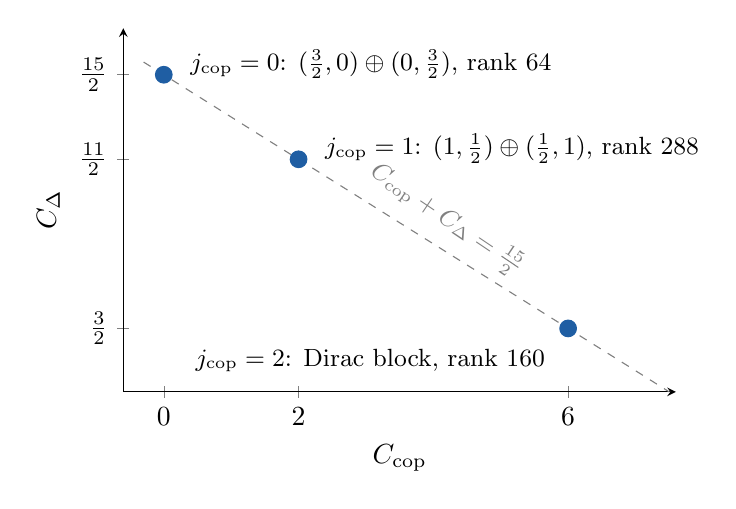
\begin{tikzpicture}
\begin{axis}[width=8.6cm,height=6.2cm,xmin=-0.6,xmax=7.6,ymin=0,ymax=8.6,
  xlabel={$C_{\rm cop}$},ylabel={$C_\Delta$},xtick={0,2,6},ytick={1.5,5.5,7.5},
  yticklabels={$\tfrac32$,$\tfrac{11}2$,$\tfrac{15}2$},axis lines=left,clip=false]
\addplot[gray,dashed,domain=-0.3:7.5] {7.5-x};
\addplot[only marks,mark=*,mark size=3pt,tcol] coordinates {(0,7.5) (2,5.5) (6,1.5)};
\node[anchor=west] at (axis cs:0.25,7.75) {\small $j_{\rm cop}=0$: $(\tfrac32,0)\oplus(0,\tfrac32)$, rank $64$};
\node[anchor=west] at (axis cs:2.25,5.75) {\small $j_{\rm cop}=1$: $(1,\tfrac12)\oplus(\tfrac12,1)$, rank $288$};
\node[anchor=north east] at (axis cs:5.8,1.25) {\small $j_{\rm cop}=2$: Dirac block, rank $160$};
\node[gray,rotate=-34,anchor=south] at (axis cs:4.0,3.6) {\small $C_{\rm cop}+C_\Delta=\tfrac{15}2$};
\end{axis}
\end{tikzpicture}
\caption{The diagonal sector at three constituents (\cref{thm:casid,cor:howe}). The copy Casimir and the Lorentz Casimir add up to a constant
on the whole module, so copy spin is locked to Lorentz type: the Dirac block is exactly the copy quintet.}
\label{fig:dualpair}
\end{figure}

A projector selected by a rotation condition alone need not be Lorentz invariant. The rotation Casimir $-\sum_{i<j}\Delta_{ij}^2$ has spectrum
$\{\tfrac34\,(256),\tfrac{15}4\,(256)\}$, and its rank-$256$ spin-$\tfrac12$ projector commutes with the rotations and with no boost: inside the
irreducible $(1,\tfrac12)$ a boost carries the $j=\tfrac12$ piece into the $j=\tfrac32$ piece. The Lorentz-invariant answer is rank $160$.

\subsection{Gamma matrices on the Dirac block}

The averaged gammas $V_\mu=3^{-1/2}\sum_k\gamma^{(k)}_\mu$ satisfy $\{V_\mu,V_\nu\}=2\eta_{\mu\nu}$ and transform as a Lorentz vector, but they are a
copy vector, not a copy singlet: they map $\mathcal D$ into itself and into the rank-$288$ block with equal norms, and their compression to
$\mathcal D$ degenerates on a rank-$32$ locus. The block does carry gamma matrices; they come from a copy-singlet cubic.

\begin{theorem}[A gauge-invariant $\Cl(1,3)$ on the Dirac block]
\label{thm:blockgamma}
Set $\Psi_{abc}=\varepsilon_{klm}\gamma^{(k)}_a\gamma^{(l)}_b\gamma^{(m)}_c$,
\[
Q_\mu=\tfrac12\eta^{\nu\rho}\Psi_{\mu\nu\rho}
=\sum_\nu\eta_{\nu\nu}\bigl(\gamma^{(1)}_\mu\gamma^{(2)}_\nu\gamma^{(3)}_\nu+\gamma^{(1)}_\nu\gamma^{(2)}_\mu\gamma^{(3)}_\nu+\gamma^{(1)}_\nu\gamma^{(2)}_\nu\gamma^{(3)}_\mu\bigr),
\qquad
G_\mu=\tfrac16\,\omega_{\mathcal S}Q_\mu\big|_{\mathcal D},
\]
with $\omega_{\mathcal S}$ the product of the six surplus generators. Then $\Psi$ is a copy singlet and totally symmetric in $(a,b,c)$; each $Q_\mu$
is a sum of ten grade-three blades, commutes with all eighteen gauge generators and with $C_\Delta$, is a Lorentz vector, and satisfies
$\{Q_\mu,Q_\nu\}|_{\mathcal D}=-72\,\eta_{\mu\nu}$. Consequently, on all $160$ dimensions,
\[
\{G_\mu,G_\nu\}=2\eta_{\mu\nu}\id_{\mathcal D},\qquad [\Delta_{ab},G_c]=\eta_{bc}G_a-\eta_{ac}G_b,\qquad [G_\mu,\mathfrak z(\Delta)]=0,\qquad
\tfrac14[G_a,G_b]=\Delta_{ab}|_{\mathcal D}.
\]
\end{theorem}

\begin{proof}
Reordering $\gamma^{(\sigma1)}\gamma^{(\sigma2)}\gamma^{(\sigma3)}$ into copy order costs $\operatorname{sign}\sigma$, because generators of distinct
constituents anticommute; against the factor $\varepsilon$ this gives $(\operatorname{sign}\sigma)^2=1$, so antisymmetry in the copies is symmetry
in the Lorentz labels. Block preservation follows because a copy singlet commutes with $C_{\rm cop}$ and hence, by \eqref{eq:casid}, with
$C_\Delta$. Finally $\omega_{\mathcal S}$ commutes with $Q_\mu$ and $\omega_{\mathcal S}^2=-\id$, so $\{G_\mu,G_\nu\}=\tfrac1{36}(-\id)(-72\eta_{\mu\nu})$.
\end{proof}

The sign flip is not cosmetic. $\Cl(1,3)\cong M_2(\HH)$ has minimal real module of dimension eight, so the four-dimensional Majorana module
carries no real $\Cl(1,3)$; the $Q_\mu$ alone generate $\Cl(3,1)$, and $\omega_{\mathcal S}$, with square $-\id$, converts them. The operator
$\slashed D=G^\mu\nabla_\mu$ is Lorentz covariant and gauge invariant on $\mathcal D$; $G_5=G_0G_1G_2G_3$ has $G_5^2=-\id$, a complex structure
rather than a chirality, as $M_2(\HH)$ requires.

\subsection{The diagonal sector is vector-like}

\begin{theorem}[Vector-likeness]
\label{thm:diagvectorlike}
Let $W_\mu=\gamma^{(1)}_\mu\gamma^{(2)}_\mu\gamma^{(3)}_\mu$. Then $W_\mu^2=-\eta_{\mu\mu}$, so $W_\mu$ is invertible; $[W_\mu,\mathfrak z(\Delta)]=0$;
$W_\mu$ anticommutes with $\Delta_{ab}$ when $\mu\in\{a,b\}$ and commutes otherwise, hence commutes with $C_\Delta$ and preserves every block;
and $W_\mu$ anticommutes with the gauge-invariant chirality $\omega=E_1\cdots E_{18}$. Therefore $W_0$ is an invertible
$\mathfrak z(\Delta)$-equivariant map exchanging the two chiral halves of every $C_\Delta$ block, and all of $S_3$ is vector-like for $\mathfrak z(\Delta)$.
\end{theorem}

\begin{proof}
Each property is \eqref{eq:bladecomm} with $|I|=3$: against a surplus bivector the sign is $(-1)^{6}$; against $M_{kl}$, the term with $\nu=\mu$
meets $W_\mu$ in two indices and the others in none; against $\Delta_{ab}$ it is $(-1)^{6-1}$ when $\mu\in\{a,b\}$; against $\omega$ it is
$(-1)^{54-3}$. The intertwining conclusion is Schur's lemma.
\end{proof}

By \cref{cor:howe} the reason is structural: $\mathcal D\cong L\otimes U$ with the gauge algebra acting on $U$ only, so chirality and gauge charge
are carried by different tensor factors. Vector-like means that the gauge representation permits a mass for every state, not that any mass is
large; nothing here fixes a scale. A Weyl projection of the block is possible, and it keeps the kinetic operators and the gauge algebra, but it
is then a choice of field content, and at three constituents it carries a colour anomaly (\cref{prop:diagtower}).

\subsection{The candidate gauge algebra of every Lorentz action}

A Lorentz action on the tower can be taken from each constituent in one of three ways: by the interior algebra $\lint$, by the algebra $\lG$
that centralises the binding operator (\cref{sec:emfield}), or not at all.

\begin{theorem}[Candidate algebras]
\label{thm:algebra}
Let the Lorentz algebra act on rung $n$ by $\lint$ on $k_I$ constituents, by $\lG$ on $k_B$ constituents and trivially on $k_S$ constituents,
$k_I+k_B\ge1$. The grade-two elements of $\Cl(3n,3n)$ commuting with the action form
\[
\mathfrak g(k_I,k_B,k_S)\cong\so{k_I}\oplus\so{2k_I+3k_S,\,3k_S}\oplus\so{k_B,\C},
\]
a direct sum of ideals. Its maximal compact subalgebra is $\so{k_I}\oplus\so{2k_I+3k_S}\oplus\so{3k_S}\oplus\so{k_B}$, and the algebra is
compact exactly when $k_S=0$ and $k_B\le1$.
\end{theorem}

\begin{proof}
Grade two is $\so{V_n}$, and $V_n=U\oplus W\oplus F$ with $U=\R^{k_I}\otimes\R^{1,3}$ the interior four-planes, $W$ the Lorentz-trivial directions
(the surplus pairs of the interior constituents and all directions of the spectators, of signature $(2k_I+3k_S,3k_S)$), and $F=\R^{k_B}\otimes V_f$ with
$V_f=(1,0)\oplus(0,1)$ the binding frames. The modules $(\tfrac12,\tfrac12)$, $\mathbf1$ and $V_f$ are pairwise inequivalent and irreducible, so
the mixed parts of $\Lambda^2V_n$ contain no invariant. $\Lambda^2W$ is invariant and gives $\so W$. In
$\Lambda^2U=(\Lambda^2\R^{k_I}\otimes S^2\R^4)\oplus(S^2\R^{k_I}\otimes\Lambda^2\R^4)$ the invariants of $S^2\R^4$ are the multiples of $\eta$ and those of
$\Lambda^2\R^4$ vanish, leaving $\so{k_I}$. On $V_f$ the invariant symmetric forms are spanned by $\eta$ and $\eta(\cdot,G\cdot)$ and there is no invariant
antisymmetric form, leaving $\Lambda^2\R^{k_B}\otimes\operatorname{span}\{\id,G\}\cong\so{k_B,\C}$.
\end{proof}

\begin{proposition}[Orthogonal against spin actions]
\label{prop:orthospin}
A copy rotation of interior four-planes is a sum of four commuting terms of square $-\tfrac14$, and one of binding frames a sum of six; their eigenvalues
on $S_n$ are $i$ times integers, and a rotation through $2\pi$ is the identity. A rotation $\tfrac12e_se_t$ of two Lorentz-trivial directions of equal
sign squares to $-\tfrac14$ and its rotation through $2\pi$ is $-\id$. The copy algebras act through orthogonal groups, the algebra of the Lorentz-trivial
directions through spin groups. Consequently the spin content of $S_n$ is half-integer if $k_I$ is odd and integer if $k_I$ is even: fermions require an
odd number of interior constituents.
\end{proposition}

\subsection{The diagonal tower}

Under the diagonal interior action the $4n$ four-plane generators and the $2n$ surplus generators $e^{(k)}_2,e^{(k)}_3$ anticommute, so
$S_n\otimes\C\cong S_{4n}\otimes S_{2n}$, with the Lorentz and copy algebras acting on the first factor and the surplus $\so{2n}$ on the second. The
connection algebra is the compact $\so n\oplus\so{2n}$, of dimension $n(5n-3)/2$.

\begin{proposition}[The diagonal tower]
\label{prop:diagtower}
\begin{enumerate}[label=(\roman*),leftmargin=2.2em]
\item For $n\le7$ the factor $S_{4n}$ decomposes under $\lint\oplus\so n$ without multiplicity. Spin is half-integer exactly at odd $n$, and the Dirac
components occur only at odd $n$, each once, tensored with the copy representation of highest weight $(2,\dots,2)$, of dimension $1,5,35,294$ at
$n=1,3,5,7$.
\item At odd $n$ the product $\mathcal J$ of the $2n$ surplus generators is a complex structure commuting with the whole connection algebra, and
$\Gamma=\mathcal J\Omega$ is a chirality. With $\mathcal J$ as $i$ the Dirac block is $[(\tfrac12,0)\oplus(0,\tfrac12)]\otimes V_{(2,\dots,2)}\otimes S^+$,
with $S^+$ a half-spinor of the surplus $\so{2n}$, and the charge $q=-\mathcal J\tilde J/2$ of $\tilde J=\sum_kJ^{(k)}$ takes on $S^+$ the values
\begin{center}
\begin{tabular}{@{}lll@{}}
\toprule
$n$ & $\dim S^+$ & values of $q$ (multiplicity)\\
\midrule
$1$ & $1$ & $\tfrac12$\\
$3$ & $4$ & $-\tfrac32\,(1)$, $\tfrac12\,(3)$\\
$5$ & $16$ & $-\tfrac32\,(5)$, $\tfrac12\,(10)$, $\tfrac52\,(1)$\\
$7$ & $64$ & $-\tfrac72\,(1)$, $-\tfrac32\,(21)$, $\tfrac12\,(35)$, $\tfrac52\,(7)$\\
\bottomrule
\end{tabular}
\end{center}
\item At $n=3$ the centraliser of $\tilde J$ in the surplus $\so6$ is $\uu3$, whose derived algebra is a compact $\su3$; on a Weyl half it acts as
a triplet with $q=\tfrac12$ and a singlet with $q=-\tfrac32$, so that with $\BmL=\tfrac23q$ the triplet has $\BmL=\tfrac13$ and the singlet $-1$:
lepton number as the fourth colour \cite{PatiSalam}. The eight gluons are neutral, the six remaining generators of $\so6$ carry $q=\pm2$ and turn
the triplet into the singlet, as leptoquark bosons do. The copy $\so3$ acts on the Dirac block with Casimir $6$, that is isospin two: it is not weak
isospin.
\item At $n=5$, with colour on three surplus planes and weak isospin on two, $S^+$ is one Standard-Model family with a right-handed neutrino,
$(\mathbf3,\mathbf2)_{1/6}\oplus(\bar{\mathbf3},\mathbf1)_{-2/3}\oplus(\bar{\mathbf3},\mathbf1)_{1/3}\oplus(\mathbf1,\mathbf2)_{-1/2}\oplus(\mathbf1,\mathbf1)_1\oplus(\mathbf1,\mathbf1)_0$,
the spinor $\mathbf{16}$ of $\so{10}$ \cite{FritzschMinkowski,Slansky}, occurring in $35$ copies. At $n=7$, $S^+$ under $\so{10}\oplus\so4$ is two
families and two mirror families, the pattern found for the spinor of $\so{18}$ \cite{WilczekZee}.
\item The Dirac block is vector-like at every odd $n$. Its Weyl projection admits no gauge-invariant mass, since no weight of $S^+$ has its negative in
$S^+$; at $n=3$ it carries a colour anomaly, $\Tr(P_L\mathcal JH^3)=960$ for the colour Cartan element $H=J^{(1)}+J^{(2)}-2J^{(3)}$, and at $n=5$ every
Standard-Model anomaly sum vanishes and $\so{10}$ has no cubic anomaly \cite{GeorgiGlashow72}.
\end{enumerate}
\end{proposition}

\begin{lemma}[No grade-two generator is chiral by itself]
\label{lem:nochiral}
Let $\Gamma$ be, up to sign, a product of $k\ge5$ distinct generators with $\Gamma^2=\id$, and $P_{L,R}=\tfrac12(\id\mp\Gamma)$. A grade-two element $X$
with $XP_R=0$ is zero.
\end{lemma}

\begin{proof}
$XP_R=0$ means $X\Gamma=-X$. For $a\neq b$, $e_ae_b\Gamma$ is a blade of grade $k-2$, $k$ or $k+2$, so $X\Gamma$ has no grade-two component, and
$X\Gamma=-X$ forces $X=0$.
\end{proof}

Under the diagonal and the spectator actions the chirality is, up to sign, the volume element of $\Cl(3n,3n)$, so a gauge interaction built from
connection components can be chiral only through the representation the Weyl block carries.

\subsection{The compact part of the spectator algebra}

Under the spectator action the connection components form $\so{3n-1,3n-3}$, noncompact for $n\ge2$, and the gauge algebra is its compact part
$\so{3n-1}\oplus\so{3n-3}$, acting through spinors. Let $w$ be the product of the $6n-4$ Lorentz-trivial generators; it commutes with the whole
connection algebra and serves as its complex structure, and $\Gamma=w\,\Omega^{(1)}$ is the chirality.

\begin{proposition}[What the spectator gauge algebra acts on]
\label{prop:spectator}
At $n=2$ the Weyl block is $(\tfrac12,0)\otimes(\mathbf4,\mathbf2)$ under $\spp2\oplus\su2\cong\so5\oplus\so3$: isospin doublets without colour, in a
real representation, so the weak interaction it carries is vector-like. At $n=3$ the Weyl block is
\[
(\tfrac12,0)\otimes\bigl[(\mathbf8_s,\mathbf4)\oplus(\mathbf8_c,\bar{\mathbf4})\bigr]\quad\text{under }\so8\oplus\so6 .
\]
With colour on three negative planes, weak isospin on two positive planes and a family $\so4$ on the remaining two, its $64$ weights are two
Standard-Model families with $\nu^c$ and two mirror families. The cubic $\su4$ sum and the Standard-Model anomaly sums vanish, there are sixteen weak
doublets, the weak roots carry $Q=\pm1$, the gluons are neutral and the leptoquarks carry $\pm\tfrac23$. The block is chiral and anomaly free under
$\so8\oplus\so6$ and vector-like under the Standard-Model algebra.
\end{proposition}

At $n=3$ the compact spectator algebra therefore already contains the Pati--Salam algebra $\so4\oplus\so6\cong\su2_L\oplus\su2_R\oplus\su4$. The
projector $P_*$ of \cref{sec:pstar} is a way of cutting one chiral family out of this content.

\subsection{Vector bosons rung by rung}
\label{sec:rungs}

\begin{center}
\small
\begin{tabular}{@{}cllcl@{}}
\toprule
$n$ & diagonal connection algebra & bosons & fermions & action on the Dirac block\\
\midrule
$1$ & $\so2=\uu1_J$ & $1$ & yes & one charge, also the complex structure\\
$2$ & $\so2\oplus\so4$ & $7$ & no & integer spin only\\
$3$ & $\so3\oplus\so6\cong\su2\oplus\su4$ & $18$ & yes & $5\times(\mathbf3\oplus\mathbf1)$; the $\su2$ is the copy algebra\\
$4$ & $\so4\oplus\so8$ & $34$ & no & ---\\
$5$ & $\so5\oplus\so{10}$ & $55$ & yes & $35\times\mathbf{16}$, one family each\\
$7$ & $\so7\oplus\so{14}$ & $112$ & yes & $294\times(2\cdot\mathbf{16}\oplus2\cdot\overline{\mathbf{16}})$\\
\midrule
$n$ & spectator gauge algebra & bosons & & action on the Weyl block\\
\midrule
$1$ & $\so2$ & $1$ & & one charge\\
$2$ & $\so5\oplus\so3$ & $13$ & & $(\mathbf4,\mathbf2)$: doublets, no colour, real\\
$3$ & $\so8\oplus\so6$ & $43$ & & two families and two mirror families\\
\bottomrule
\end{tabular}
\end{center}
The tempting assignment ``$n=1$: photon; $n=2$: $W$ and $Z$; $n=3$: gluons'' can now be tested. The photon at $n=1$ is supported: the single
connection component $J$ gauges the Dirac spinor and is also its complex structure. Chiral $W$ and $Z$ at $n=2$ are supported by no action: the
diagonal action has no fermions there, the action that is interior on one constituent and binding on the other has the abelian algebra $\uu1$ only, and
the spectator Weyl block is a real representation. Gluons at $n=3$ are supported, without weak bosons under the diagonal action, where the $\su2$ is
the copy algebra, and with them under the spectator action. Rung three is the first at which some gauge algebra contains
$\su3\oplus\su2\oplus\uu1$ acting on fermions in Standard-Model representations, there together with mirror families; among the actions with a compact
connection algebra the first such rung is $n=5$, through $\so{10}$, with one family per copy and thirty-five copies. Nothing computed here reduces the
copy multiplicity to three, and the rung index counts tensor factors, so none of this identifies particles with constituents.

\part{Gauge fields and the electromagnetic reading}
\section{The projector as a field}
\label{sec:fields}

Up to this point a projector has been a choice made once and for all. A choice of this kind becomes a field as soon as it is
allowed to vary from point to point, and the selection problem then changes character: instead of asking which projector is
right we ask which configurations an action prefers. Before any action can be written, three things must be known: the space in
which the projector moves, the connection it induces on its own image, and the sign of the natural metric on its variations. All
three can be computed exactly, and each of them carries a surprise.

\subsection{Configuration space}

Let $\mathcal P_r$ be the set of orthogonal projectors $P$ on $S_3=\R^{512}$ of rank $r$ that commute with the interior Lorentz
action $\Sigma$. Differentiating $P^2=P$ gives $dP\,P+P\,dP=dP$, hence
\[
P\,dP\,P=0,\qquad (\id-P)\,dP\,(\id-P)=0 :
\]
a variation of a projector is purely off-diagonal with respect to the splitting $\operatorname{im}P\oplus\ker P$. The tangent space
is therefore
\[
T_P\mathcal P_r=\bigl\{S:\ S^{\!\top}=S,\ PSP=0,\ (\id-P)S(\id-P)=0,\ [S,\Sigma]=0\bigr\},
\]
the tangent space of the real Grassmannian cut down by the Lorentz condition.

\begin{proposition}[Configuration space]
\label{prop:config}
The Lorentz commutant $\mathcal C\subset\End_\R(S_3)$ is spanned by the $32768$ blades that commute with the six interior
bivectors. Its centre is $\{\id,\Omega\}\cong\C$ with $\Omega=\gamma^0\gamma^1\gamma^2\gamma^3$, $\Omega^2=-\id$, and since a
semisimple real algebra of dimension $2\cdot128^2$ with centre $\C$ is $M_{128}(\C)$, we have $\mathcal C\cong M_{128}(\C)$.
Consequently
\[
\mathcal P_r\cong\mathrm{Gr}_\C\bigl(\tfrac r4,128\bigr),\qquad
\dim_\R\mathcal P_r=2\,\frac r4\Bigl(128-\frac r4\Bigr),
\]
which is $3584$ at $r=64$ and $6144$ at $r=128$, against $\dim\mathrm{Gr}_\R(64,512)=28672$ for the unconstrained real Grassmannian.
\end{proposition}

The complex structure that appears here is the interior volume $\Omega$, not the internal one $\omega_I$ of \cref{thm:i}. That is
not a contradiction. The commutant of the Lorentz action alone contains $e^{(1)}_2$, which commutes with the six interior bivectors
but anticommutes with the fourteen-index volume $\omega_I$, so $\omega_I$ is not central in $\mathcal C$; it becomes central only in
the smaller algebra that also commutes with the internal bivectors, which is the algebra of \cref{thm:i}. Each structure is central
in its own ambient algebra, which is the pattern described after \cref{prop:6plus8plus1}.

\begin{remark}[No blade is tangent]
\label{rem:noblade}
A count of tangent directions by blades fails, for a reason worth recording. Let $P=\prod_i\tfrac12(\id+X_i)$ be one of the
projectors of \cref{sec:projectors}, built from $k$ commuting involutions, and let $B$ be a blade anticommuting with at least one
$X_i$. Then $PBP=0$, but $(\id-P)B(\id-P)=(\id-P-P_\varepsilon)B$ with $P_\varepsilon=\prod_i\tfrac12(\id+\varepsilon_iX_i)$, which
vanishes only when $P+P_\varepsilon=\id$, that is only for $k=1$. There is also a rank argument: a blade is a signed permutation matrix,
invertible of rank $512$, while a tangent vector has the block form $\bigl(\begin{smallmatrix}0&A^{\!\top}\\A&0\end{smallmatrix}\bigr)$ and
rank at most $2r$. For $k\ge2$ no single blade is tangent, the tangent space is not spanned by blades, and a blade count
overestimates it, by a factor four at $r=64$ and two at $r=128$. The dimensions of \cref{prop:config} are obtained by imposing
both conditions sector by sector.
\end{remark}

\subsection{The sign of a variation}

The group that the geometry supplies is generated by the internal bivectors, and it moves a projector along an orbit inside
$\mathcal P_r$. Whether a bivector moves $P$ to another orthogonal projector, and with what sign the natural trace form measures
the motion, is decided by the signature rule of \cref{thm:sig}.

\begin{theorem}[The trace form splits by the Cartan involution]
\label{thm:ghost}
Let $P=P^{\!\top}=P^2$, let $B$ be a bivector and $T=[B,P]$. Then $T^{\!\top}=PB^{\!\top}-B^{\!\top}P$, and
\begin{enumerate}[label=(\roman*),leftmargin=2.2em]
\item if $B$ is compact, $B^{\!\top}=-B$, then $T$ is symmetric and $\Tr(T^2)=\Tr(T^{\!\top}T)>0$ unless $T=0$;
\item if $B$ is a boost, $B^{\!\top}=B$, then $T$ is antisymmetric and $\Tr(T^2)=-\Tr(T^{\!\top}T)<0$ unless $T=0$.
\end{enumerate}
Symmetric and antisymmetric matrices are trace-orthogonal, so on an orbit the trace form is an orthogonal sum of a positive
definite piece on the directions generated by compact bivectors and a negative definite piece on those generated by boosts. Only
the former are tangent to the manifold of orthogonal projectors.
\end{theorem}

\begin{proof}
$T^{\!\top}=(BP-PB)^{\!\top}=PB^{\!\top}-B^{\!\top}P$, which is $T$ when $B^{\!\top}=-B$ and $-T$ when $B^{\!\top}=B$. The trace of the
product of a symmetric and an antisymmetric matrix vanishes. A curve of orthogonal projectors has symmetric velocity, so the
antisymmetric directions leave that manifold.
\end{proof}

\begin{example}[The paired-mode projector at one constituent]
\label{ex:ghostPi}
Take the rank-four projector $\Pi$ of \cref{ex:pairedmode}. Its stabiliser in $\so{3,3}$ has dimension nine, so its orbit has
dimension six. On the bivectors
\[
B_I=\tfrac12\bigl(e_1e_2,\ e_1e_3,\ e_2e_3,\ e_1e_5,\ e_1e_6,\ e_2e_6\bigr),\qquad T_I=[B_I,\Pi],
\]
an exact $8\times8$ computation gives $\Tr(T_IT_J)=\operatorname{diag}(1,1,1,-1,-1,-1)$. The first three $B_I$ are time--time rotations,
the last three are boosts, exactly as \cref{thm:ghost} predicts. Only three of the fifteen basis bivectors commute with $\Pi$
individually, while the stabiliser has dimension nine, so six of its directions are combinations of basis bivectors and no single
one of them. Reading a stabiliser off basis elements overestimates the orbit.
\end{example}

Positive norm and tangency are nevertheless different conditions. For unit $T_{\rm sym}$ and $T_{\rm anti}$ of the two kinds,
$\Tr\bigl((T_{\rm sym}+\tfrac12T_{\rm anti})^2\bigr)=1-\tfrac14>0$, yet the direction is not symmetric and leaves the orthogonal
projectors. What is exact is the orthogonal splitting, not an equivalence between the sign of the norm and tangency. On the manifold
of orthogonal projectors itself every variation is symmetric and the trace form is positive definite, so the indefiniteness of the
example is an artefact of moving $\Pi$ along the full $\mathrm{Spin}(3,3)$ orbit. This is a statement about the target of a
projector field and not about a field theory over a base: in a base of split signature the kinetic contraction
$g^{\mu\nu}\Tr(D_\mu P\,D_\nu P)$ is indefinite in the spacetime index whatever the target metric is.

At three constituents the same reasoning counts the physical motions of $\Pfam$. Of the $91$ internal bivectors $43$ are compact,
forming the maximal compact $\so8\oplus\so6$, and the compact part of the stabiliser of $\Pfam$ has dimension nine
(\cref{thm:table}), so the compact orbit through $\Pfam$ has dimension
\[
43-9=34 ,
\]
which is also the rank of $B\mapsto[B,\Pfam]$ on the compact bivectors. Only seven of the $43$ compact basis bivectors commute with
$\Pfam$ individually, which repeats the warning of \cref{ex:ghostPi}. Of the $3584$ configuration directions at rank $64$,
thirty-four lie along the only group the geometry supplies. Whether these thirty-four are gauge redundancies or physical modes is a
question about an action, which the algebra does not supply.

\subsection{The induced connection over-generates}

A varying projector carries its own connection. If the gauge field is not postulated but induced, $\nabla=P\,d$ on the bundle of
images, then its curvature $F_{\mu\nu}=P[\partial_\mu P,\partial_\nu P]P$ is a composite, and the algebra in which it takes values is
computed rather than chosen. To leading order in the Ambrose--Singer theorem that algebra is
\[
\mathfrak h(P)=\operatorname{span}\bigl\{P[S,S']P:\ S,S'\in T_P\mathcal P_r\bigr\}.
\]

\begin{theorem}[Over-generation]
\label{thm:holonomy}
Let $P(x)$ range over all of $\mathcal P_{64}$. The curvature values $P[\partial_\mu P,\partial_\nu P]P$ are antisymmetric, hence
compact, and lie in the block, and their span on $\operatorname{im}\Pfam$ has dimension
\[
\dim\mathfrak h(\Pfam)=256=\dim\uu{16},
\]
the largest compact algebra the block admits at all. It exceeds the six dimensions of $\keff(\Pfam)=\uu1^3\oplus\su2$ by a factor
of about $43$.
\end{theorem}

The induced connection is not flat, every curvature value is compact, and every value lies in the block. The route fails by
over-generating and by nothing else. In particular chirality is not among the casualties.

\begin{proposition}[Chirality must be imposed, and costs nothing]
\label{prop:chiralpreserved}
Every projector of the family commutes with $\Gamma$. If a field $P(x)$ is required to satisfy $[P(x),\Gamma]=0$ everywhere, then
$[\partial_\mu P,\Gamma]=0$ and
\[
\bigl[P[\partial_\mu P,\partial_\nu P]P,\ \Gamma\bigr]=0 ,
\]
so the induced curvature preserves chirality and the holonomy lies in $\uu8\oplus\uu8$. That algebra is still far larger than
$\uu1^3\oplus\su2$.
\end{proposition}

The comparison of \cref{thm:holonomy} is between what the construction permits and what is wanted, not an impossibility theorem
about any particular field. A constant field has zero induced curvature, and a field compatible with $\Gamma$ has holonomy inside
$\uu8\oplus\uu8$. What the comparison does establish is the direction of the problem. A parent action must \emph{cut} the freedom of
the projector, by a constraint that shrinks $T_P\mathcal P$ before the curvature is formed or by a potential that freezes all but the
intended holonomy directions, rather than build a gauge field up from nothing. This reverses the usual motivation for composite
gauge fields. \Cref{fig:freedom} collects the numbers.

\begin{figure}[t]
\centering
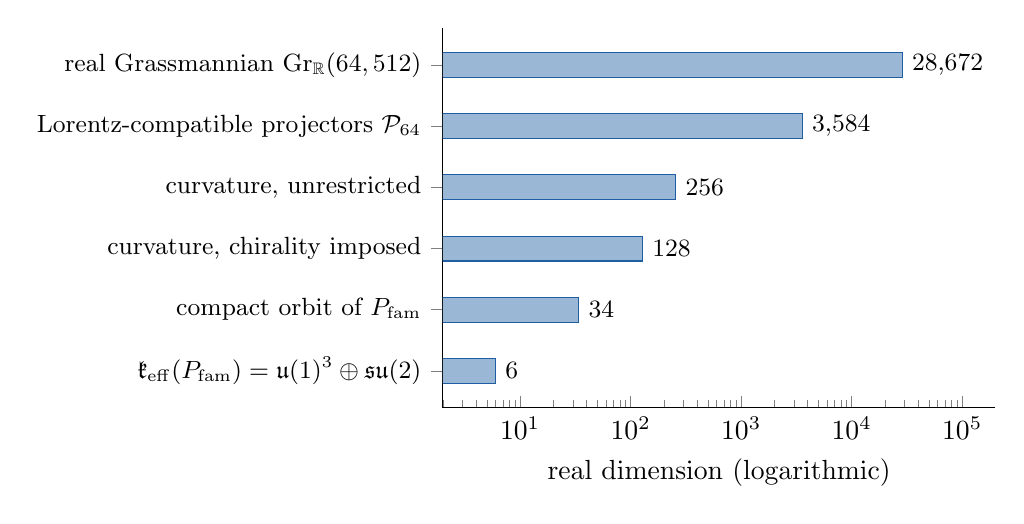
\begin{tikzpicture}
\begin{axis}[xbar,xmode=log,log basis x=10,width=8.6cm,height=6.4cm,
  xmin=2,xmax=200000,
  ytick=data,
  symbolic y coords={keff,orbit,u8u8,u16,P64,GrR},
  yticklabels={{$\keff(\Pfam)=\uu1^3\oplus\su2$},{compact orbit of $\Pfam$},{curvature, chirality imposed},{curvature, unrestricted},{Lorentz-compatible projectors $\mathcal P_{64}$},{real Grassmannian $\mathrm{Gr}_\R(64,512)$}},
  yticklabel style={font=\small},
  xlabel={real dimension (logarithmic)},
  bar width=9pt,
  nodes near coords,
  nodes near coords style={font=\small,anchor=west},
  point meta=rawx,
  enlarge y limits=0.12,
  axis x line*=bottom, axis y line*=left]
\addplot[fill=tcol!45,draw=tcol] coordinates {(6,keff) (34,orbit) (128,u8u8) (256,u16) (3584,P64) (28672,GrR)};
\end{axis}
\end{tikzpicture}
\caption{How much freedom a projector field has at rank $64$, and how little of it is wanted. The configuration space of
Lorentz-compatible projectors (\cref{prop:config}) is far smaller than the real Grassmannian but still enormous; the group the
geometry supplies moves $\Pfam$ along only $34$ directions; and the curvature algebra the induced connection can reach
(\cref{thm:holonomy,prop:chiralpreserved}) exceeds the faithful gauge algebra of the block by more than an order of magnitude.}
\label{fig:freedom}
\end{figure}

\subsection{One explicit variational model}
\label{sec:trialaction}

A list of fields does not determine field equations. What can be done without a derived action is to adopt one explicitly, derive
its equation, and record what it can and cannot do. On a four-dimensional Lorentzian base, with $D_\mu P=\partial_\mu P+[A_\mu,P]$ and
with $f$ and $V$ as inputs, take
\begin{equation}
\label{eq:trialS}
S_P=\int\sqrt{-g}\,\Bigl(\tfrac{f^2}2\Tr\bigl(D_\mu P\,D^\mu P\bigr)-V(P)\Bigr).
\end{equation}
Varying along the Grassmannian, $\delta P=[\epsilon,P]$ with $\epsilon$ antisymmetric, gives
\begin{equation}
\label{eq:Pieom}
\bigl[P,\ f^2D_\mu D^\mu P+V'(P)\bigr]=0 ,
\end{equation}
and for $V=0$ this is the conservation law $D_\mu\mathcal C^\mu=0$ of the matrix current $\mathcal C_\mu=[P,D_\mu P]$. The variation
has to be projected onto the admissible tangent space whenever $P$ is restricted further, for instance to commute with $\Gamma$.

Three consequences are immediate. First, a potential that depends only on the spectrum of a projector of fixed rank is constant,
since $\Tr f(P)=rf(1)+(d-r)f(0)$; such a potential selects nothing, and for the pure kinetic term every constant admissible projector
is a critical point. Selection needs couplings that distinguish orbits, and there is more than one orbit to distinguish: at rank
$64$ the orbits through $\Pfam$ and $P_*$ have dimensions $34$ and $20$ (\cref{prop:orbits}). Second, whether varying $A_\mu$ gives a
Yang--Mills equation depends on how the action depends on $A$, not on $A$ appearing in a list of fields; a composite $A$ contributes
through the chain rule to the equations of its constituents. Third, the pointwise stabiliser condition $[A_\mu,P]=0$ is not the
condition $D_\mu P=0$ that a moving subbundle be preserved; the two agree only for constant $P$. Which connection acts on matter,
$P(d+A)$, an ambient connection preserving $P$, or an independent connection in a moving frame of the block, is a further choice,
and we make none of them here.

\subsection{What Yang--Mills theory keeps open}
\label{sec:ym}

Four conditions on a connection have been established as theorems: commutation with the Lorentz action
(\cref{thm:centraliser}); commutation with the projector, with a faithful action on its image (\cref{def:keff,thm:table});
antisymmetry, which for bivectors is \cref{thm:sig}; and preservation of the kinetic kernels $K^\mu$. They are homogeneous and
geometric, and together they determine the algebra in which $A_\mu$ takes its values, $\uu1^3\oplus\su2$ on the family block,
$\so6\oplus\su2^{\oplus3}$ at rank $256$ and the Pati--Salam algebra on $P_*$, over the single frame of \cref{prop:frame}. They do not
determine the field, since no parent action is derived; nor the couplings, since homogeneous conditions cancel every
normalisation; nor which abelian direction is electromagnetic, by \cref{thm:pairing}.

There is no representational obstruction behind this. By the theorem on universal connections \cite{NarasimhanRamanan}, every
connection on a bundle over a manifold of bounded dimension is the pullback of the canonical connection of a tautological bundle
over a Grassmannian of sufficient rank, so the projector representation of a gauge field is always available in principle. The
difficulty is dynamical, and power counting makes it concrete. A projector is dimensionless, so $\Tr(\partial P\,\partial P)$
carries a coupling of mass dimension $D-2$ and $\Tr F^2$ one of dimension $D-4$. In two dimensions the sigma model is
renormalisable and the composite gauge field acquires a kinetic term at leading order in $1/N$, with linear confinement of the
constituents \cite{DAddaDiVecchiaLuscher,Witten79}. In four dimensions the sigma model is not power-counting renormalisable and that
argument does not transfer.

Confinement is a separate question again. Invariant tensors permit meson-like and baryon-like operators, but they say nothing
about masses or about the energy of separated sources, and the diagnostics with dynamical matter are flux-tube and string-breaking
correlation matrices \cite{Bali05}. Moreover a block supplies a multiplicity index, not three constituents: three copies of a doublet
form a direct sum, whereas three constituents require a tensor product with antisymmetrisation, so even the operator statement needs
a Fock construction first.

\section{The split space as a space of field strengths}
\label{sec:emfield}

The arena was introduced with an electromagnetic picture in mind: six directions, three of one sign and three of the other, paired
one to one like the components of a magnetic and an electric field. This section turns the picture into a theorem and measures its
price. The binding root $G$ of \cref{prop:twoK} is the key, and its role in the interior dynamics, where it is the operator that
makes bound motion possible, is established in \cref{sec:neutral}. Here it is used only as a linear map with $G^2=-\id$ and
$G=G^\dagger$.

\subsection{Arithmetic first}

The space $\Lambda^2\R^{1,3}$ with the induced metric $\langle\theta^a\wedge\theta^b,\theta^a\wedge\theta^b\rangle=\eta^{aa}\eta^{bb}$ is
negative on the three planes $\theta^0\wedge\theta^i$ and positive on the three planes $\theta^j\wedge\theta^k$. It therefore has
signature $(3,3)$, the Lorentz group acts on it by the adjoint representation, and the Hodge star satisfies $\star^2=-\id$. This is
counting, and it must be said before anything is built on it: every six-dimensional space of split signature is isometric to a
Lorentzian field-strength space, so exhibiting one isometry predicts nothing. What is not arithmetic is which subalgebra
$\so{1,3}\subset\so{3,3}$ realises the action, and whether the operator playing the Hodge star is one the arena already had.

\subsection{The Lorentz algebra of the binding root}

\begin{theorem}[The centraliser of $G$]
\label{thm:GLorentz}
The centraliser $\lG$ of $G$ in $\so{3,3}$ is isomorphic to $\so{3,\C}\cong\slr{2,\C}\cong\so{1,3}$. Its maximal compact
subalgebra is the $\so3$ of \emph{diagonal} rotations, each acting identically on a temporal plane $(e_i,e_j)$ and on its spatial
partner $(e_{i+3},e_{j+3})$.
\end{theorem}

\begin{proof}
Since $G^2=-\id$, the identification $z_j=x_j+ix_{j+3}$ makes $\R^6$ a complex space $\C^3$ on which $G$ acts as $i$, and
commuting with $G$ is $\C$-linearity. Under this identification
\[
\eta(X,X)=\sum_jx_j^2-\sum_jx_{j+3}^2=\Re q(z),\qquad q(z):=\sum_jz_j^2,
\]
with $q$ holomorphic. A $\C$-linear map $A$ preserving $\Re q$ preserves it on every phase rotation $e^{i\vartheta}z$, and
$q(e^{i\vartheta}z)=e^{2i\vartheta}q(z)$, so $\Re\bigl(e^{2i\vartheta}[q(Az)-q(z)]\bigr)=0$ for all $\vartheta$ forces $q(Az)=q(z)$. The
group is $O(3,\C)$ and its algebra $\so{3,\C}$, whose underlying real Lie algebra is $\slr{2,\C}\cong\so{1,3}$ with maximal compact
$\so3$. A rotation of $(e_i,e_j)$ alone does not commute with $G$, because $G$ carries $e_i$ to $e_{i+3}$; only the rotation
performed identically on the partner plane does.
\end{proof}

\begin{proposition}[Two Lorentz algebras, not conjugate]
\label{prop:notconj}
The interior algebra $\lint$ and $\lG$ are isomorphic as Lie algebras but not as subalgebras of $\so{3,3}$. The interior algebra
fixes the two-dimensional surplus plane pointwise, while $\lG$ contains simultaneous rotations of both triples and has no nonzero
common fixed vector. Conjugation preserves the dimension of the common fixed subspace, so the two are not conjugate in $GL(6,\R)$,
let alone in $O(3,3)$.
\end{proposition}

Write $L_i$ for the diagonal rotations and put, for cyclic $(i,j,k)$, $K_i=\tfrac12\bigl(e_ke_{j+3}-e_je_{k+3}\bigr)$. The six
operators $L_i,K_i$ span $\lG$.

\begin{theorem}[The field-strength reading]
\label{thm:emfield}
Write a vector of $\R^{3,3}$ as $X=\sum_i\bigl(B_ie_i+E_ie_{i+3}\bigr)$. Then
\[
[L_i,L_j]=\epsilon_{ijk}L_k,\qquad [L_i,K_j]=\epsilon_{ijk}K_k,\qquad [K_i,K_j]=-\epsilon_{ijk}L_k,
\]
both triples $\bB$ and $\bE$ transform as vectors under the $L_i$, and the $K_i$ act by
\begin{equation}
\label{eq:emboost}
\delta\bE=\bv\times\bB,\qquad \delta\bB=-\bv\times\bE .
\end{equation}
Identify $X$ with the two-form $F_X$ of components $(F_X)_{0i}=E_i$ and $(F_X)_{jk}=\epsilon_{ijk}B_i$. Then $G$ is the Hodge star,
$F_{GX}=\star F_X$ with $(\star F)_{ab}=\tfrac12\varepsilon_{abcd}F^{cd}$ and $\varepsilon_{0123}=+1$, and
\[
\eta(X,X)=|\bB|^2-|\bE|^2,\qquad \eta(X,GX)=-2\,\bE\cdot\bB
\]
are the only invariant quadratic forms. With $\lG$ as its Lorentz algebra, $\R^{3,3}$ \emph{is} $\Lambda^2\R^{1,3}$.
\end{theorem}

The orientation matters once, and we fix it here. With $F_{jk}=\epsilon_{ijk}B_i$ the vector $\bB$ is minus the textbook magnetic
field of the convention $F_{jk}=-\epsilon_{ijk}B_i$ \cite{Jackson}, so we write $\Btext=-\bB$, as announced in \cref{sec:conventions};
the electric field is the textbook one. Passing to a frame moving with velocity $\mathbf u$ changes the frame variables by
$\delta\bB=\mathbf u\times\bE$ and $\delta\bE=-\mathbf u\times\bB$, which is \eqref{eq:emboost} with $\bv=-\mathbf u$; in textbook
variables this is $\bE'=\bE+\mathbf u\times\Btext$ and $\Btext'=\Btext-\mathbf u\times\bE$, the familiar first-order transformation.

\begin{example}[A boost along the third axis]
\label{ex:emboost}
Take the pure magnetic field $X=e_1$, that is $\bB=(1,0,0)$ and $\bE=0$, and the boost generator $K_3=\tfrac12(e_2e_4-e_1e_5)$,
acting on vectors by the commutator. Since $e_1$ anticommutes with $e_2$ and with $e_4$ it commutes with $e_2e_4$, while
$[e_1e_5,e_1]=-2e_1^2e_5=-2e_5$; hence $[K_3,e_1]=e_5$. Under $\delta X=\delta\,[K_3,X]$ the field acquires $\bE=(0,\delta,0)$, in accordance
with $\delta\bE=\bv\times\bB$ for $\bv=(0,0,\delta)$. In the same way $[K_3,e_5]=e_1$, so a pure electric field $\bE=(0,1,0)$ acquires
$\bB=(\delta,0,0)=-\bv\times\bE$. The invariant $\eta(X,X)=|\bB|^2-|\bE|^2$ changes only at
second order, as it must.
\end{example}

\begin{corollary}[The invariant complex structure]
\label{cor:Gselected}
$\R^6$ is irreducible under $\lG$, and the commutant of $\lG$ in $\End(\R^6)$ is $\operatorname{span}\{\id,G\}\cong\C$. Hence, once
$\lG$ is taken as the Lorentz algebra, its invariant complex structure is $\pm G$ and nothing else. The interior algebra, by contrast,
has a commutant of dimension five, $\R$ on the four-plane and all of $M_2(\R)$ on the surplus plane.
\end{corollary}

The logic of this corollary runs from $G$ to $\lG$ and back to $\pm G$, so the choice of $G$ is recovered, not removed. It is a
consistency statement, a uniqueness conditional on taking $\lG$ as the Lorentz algebra. Removing the choice would require a
characterisation of $\lG$ that does not mention $G$, and we know none.

\subsection{The two readings exclude one another}

The price of the field-strength reading is not small.

\begin{proposition}[Exclusion]
\label{prop:emexclusive}
Under $\lint$ the six directions decompose as $V\oplus2\cdot\mathbf1$, a four-vector and two scalars; under $\lG$ they are
irreducible, with no fixed vector. The two representations are not similar, so a single theory cannot use both algebras as the
Lorentz action on the same six directions. If the vector space $\R^{3,3}$ is read as the electromagnetic field strength, those six
directions are not a four-plane plus a surplus pair, and the Dirac structure, the projector census, $P_*$ and the diagonal sector
all lose the arena on which they are built.
\end{proposition}

What is excluded is reading one six-dimensional space in two ways, not a theory that contains both kinds of module. A theory may
contain spacetime vectors and field strengths as different representations of one Lorentz algebra, which is the ordinary
arrangement, and $\Cl(3,3)$ realises it with the vectors at grade one and the field strength at grade two.

\begin{proposition}[The field strength at grade two]
\label{prop:bivectorF}
Let $\Lambda^2E$ be the span of the six bivectors of the interior four-plane. It is closed under the adjoint action of $\lint$, on
which it is the adjoint representation; the trace form $\tfrac18\Tr(XY)$ on it has signature $(3,3)$; and the interior volume
$\Omega=\gamma^0\gamma^1\gamma^2\gamma^3$, with $\Omega^2=-\id$, commutes with $\lint$, preserves $\Lambda^2E$ by left multiplication,
exchanges $\gamma^0\gamma^i$ with the spatial bivectors and acts on $\Lambda^2E$ as the Hodge star.
\end{proposition}

Grade three behaves differently under the two algebras, and the difference sharpens the exclusion. Under $\lG$ one has
$(\Lambda^3\R^6)_\C=2\,(0,0)\oplus2\,(1,1)$, of dimension $2+18$, so no field-strength module $(1,0)\oplus(0,1)$ occurs at grade three
at all: trivectors cannot carry the field for this action. Under $\lint$, $\R^6=E\oplus\R^2$ gives $\Lambda^3\R^6\cong2E\oplus2\Lambda^2E$,
which contains two field-strength modules. The quadratic Casimir distinguishes the cases cleanly, with spectrum $\{0^{(2)},8^{(18)}\}$
on $\Lambda^3\R^6$ under $\lG$ and $\{3^{(8)},4^{(12)}\}$ under $\lint$, the value $4$ being that of $(1,0)\oplus(0,1)$ and $3$ that of a
four-vector. An explicit attempt confirms it: the six trivectors $C_i=\sum_{j,k}\epsilon_{ijk}e_jN_k$, $N_j=e_{k+3}e_{l+3}$ cyclically,
together with $D_i=\mathcal VC_i$, transform as two vectors under the $L_i$, but all eighteen brackets $[K_i,C_j]$, $[K_i,D_j]$ leave
their span, for instance $\tfrac12[K_1,C_1]=e_2e_3e_4+e_4e_5e_6$, and the Lorentz closure of the span has dimension $18$.

\subsection{How much of Maxwell's theory is forced}
\label{sec:maxwell}

\Cref{thm:emfield} supplies a field with the right transformation law and nothing that the field satisfies. How much of the
dynamics does the transformation law fix by itself? The answer is: the form of the equations completely, and nothing else.

\begin{theorem}[Exactly two first-order covariant operators]
\label{thm:twoops}
Consider linear first-order differential operators with constant coefficients on Minkowski space, acting on a field $F$ valued in
$\Lambda^2\R^{1,3}$ and taking values in the vector representation. The derivative $\partial F$ lies in $\Lambda^2\otimes V$, of
dimension $24$, and under $\so{1,3}$
\[
\Lambda^2\otimes V=\underbrace{(\tfrac32,\tfrac12)\oplus(\tfrac12,\tfrac32)}_{16}\ \oplus\ \underbrace{2\,(\tfrac12,\tfrac12)}_{8},
\]
so the vector module occurs with multiplicity exactly two, and no other module of dimension four occurs. The two copies are realised
by
\[
(dF)_{\mu\nu\rho}=3\,\partial_{[\mu}F_{\nu\rho]}\quad(\text{through }\Lambda^3\cong V),\qquad (\delta F)_\nu=\partial^\mu F_{\mu\nu},
\]
and every covariant operator of the class is $\mathcal DF=a\,\delta F+b\,\delta(\star F)$, since $\delta\star=\pm\star d$.
\end{theorem}

The Casimir operator confirms the count: on $\Lambda^2\otimes V$ its spectrum is $\{3^{(8)},9^{(16)}\}$, and the value $3$ is the
vector one. Nothing in the theorem constrains operators of higher order, operators with variable coefficients, or operators valued
in the remaining $(\tfrac32,\tfrac12)\oplus(\tfrac12,\tfrac32)$.

\begin{corollary}[The form of Maxwell's equations]
\label{cor:maxwellform}
Within this class the two available equations are $dF=\mathcal J_m$ and $d\star F=\mathcal J_e$. Covariance does not rule out a
magnetic current, which is a covariant field exactly as an electric current is; it identifies the two operators and leaves open
which equations are imposed and which sources are admitted. The source-free system $dF=\delta F=0$ is the only choice that needs no
external data, and within this linear class it is the only one invariant under duality, because the Hodge star $G$ exchanges the two
operators. Finally, on a contractible region $dF=0$ gives $F=dA$ by the Poincar\'e lemma, so the gauge potential is a consequence of
the first equation rather than an assumption.
\end{corollary}

In the variables of the frame the system takes a compact form, which we use repeatedly below.

\begin{proposition}[Maxwell's equations on the frame]
\label{prop:RS}
Read $\R^{3,3}$ as $\C^3$ through $G$, $z_j=B_j+iE_j$. Then $dF=0$ and $d\star F=0$ for the two-form $F_X$ of
\cref{thm:emfield} are
\begin{equation}
\label{eq:RS}
\partial_tX=-G\,(\curl X),\qquad \nabla\cdot X=0,
\end{equation}
that is $\partial_tz=-i\,\curl z$ and $\nabla\cdot z=0$, with the curl built from the rotation generators $L_i$. Splitting into the
two triples gives $\partial_t\bB=\curl\bE$, $\partial_t\bE=-\curl\bB$ and $\nabla\cdot\bE=\nabla\cdot\bB=0$; in textbook variables these
are Faraday's law $\partial_t\Btext=-\curl\bE$ and the Amp\`ere--Maxwell law $\partial_t\bE=\curl\Btext$ in vacuum. With a source,
$\partial_\mu F^{\mu\nu}=(\rho,\bj)$ reads
\begin{equation}
\label{eq:RSsource}
\partial_tz=-i\,\curl z-i\,\bj,\qquad \nabla\cdot z=i\rho ,
\end{equation}
and taking the divergence of the first equation gives $\partial_t\rho+\nabla\cdot\bj=0$: continuity is a consequence of the system and
the compatibility condition that any proposed current must satisfy.
\end{proposition}

Up to a factor $i$, $z$ is the Riemann--Silberstein vector $\bE+i\Btext$, which obeys
$i\partial_t(\bE+i\Btext)=\curl(\bE+i\Btext)$ \cite{Silberstein1907,BialynickiBirula13}, and the holomorphic form of the proof of
\cref{thm:GLorentz} has
\[
\Re q(z)=|\bB|^2-|\bE|^2,\qquad \Im q(z)=2\,\bE\cdot\bB ,
\]
so the two Maxwell invariants are the real and imaginary parts of one holomorphic quadratic form. Three classical facts fall into
place. The duality rotation is the phase rotation $z\mapsto e^{i\vartheta}z$ that the proof of \cref{thm:GLorentz} already used, and
it turns the pair of invariants by $2\vartheta$. The two quadratic forms that will compete in the interior dynamics of
\cref{sec:shifted,sec:neutral} reappear with physical names: the $\eta$-form $\Re q$ is the Lorentz invariant, while the Hermitian
form $|z|^2=|\bB|^2+|\bE|^2$ is twice the energy density and depends on the frame. And the remaining sesquilinear covariant is the
Poynting vector, $\tfrac i2\,\bar z\times z=\bE\times\bB$, so that $\bE\times\Btext=-\tfrac i2\,\bar z\times z$.

\begin{example}[A circularly polarised wave on the frame]
\label{ex:circular}
The field $z=(1,i,0)\,e^{ik(x_3-t)}$ solves \eqref{eq:RS}: $\nabla\cdot z=0$ because $z$ has no third component, and
$\curl z=ik\,(-i,1,0)e^{ik(x_3-t)}=k\,(1,i,0)e^{ik(x_3-t)}$, so $-i\curl z=-ik\,z=\partial_tz$. Its invariant is
$q(z)=(1+i^2)e^{2ik(x_3-t)}=0$, so $|\bB|=|\bE|$ and $\bE\cdot\bB=0$ at every point: the wave is null. Its Poynting vector
$\tfrac i2\bar z\times z=\tfrac i2(1,-i,0)\times(1,i,0)=\tfrac i2(0,0,2i)=(0,0,-1)$ is $\bE\times\bB$, so $\bE\times\Btext=(0,0,1)$
points along the direction of propagation, as it should.
\end{example}

\subsection{Frame vectors as spacetime planes}

Each pairing plane $(e_i,e_{i+3})$ carries one complex component $z_i=B_i+iE_i$, and a frame vector is at the same time a bivector of
spacetime. The two descriptions meet in the following way.

\begin{proposition}[Frame vectors as planes]
\label{prop:planes}
Let $X=\sum_i(B_ie_i+E_ie_{i+3})$ and $F_X$ as above. Then $\Pf F_X=\bE\cdot\bB$ and $\det F_X=(\bE\cdot\bB)^2$. A nonzero $F_X$ is a
single plane $u\wedge v$ exactly when $\bE\cdot\bB=0$, that is when $\Im q=0$. Otherwise there is a Lorentz frame in which
$F_X=a\,\theta^0\wedge\theta^1+b\,\theta^2\wedge\theta^3$ is a pair of orthogonal planes, and the duality rotation $e^{-\vartheta G}$ with
$\tan\vartheta=a/b$ carries it to the single plane $\sqrt{a^2+b^2}\,\theta^2\wedge\theta^3$, the complexion of Rainich and of Misner
and Wheeler \cite{Rainich1925,MisnerWheeler57}.
\end{proposition}

\Cref{fig:qplane} shows the content of this proposition in the plane of the complex invariant. The real axis is the locus of single
planes, the positive half of magnetic type and the negative half of electric type, the origin is the null cone, and the duality
rotation moves a field around a circle at twice its own angle. In \cref{sec:neutral} the bound orbits of the interior dynamics will
turn out to be exactly such rotations.

\begin{figure}[t]
\centering
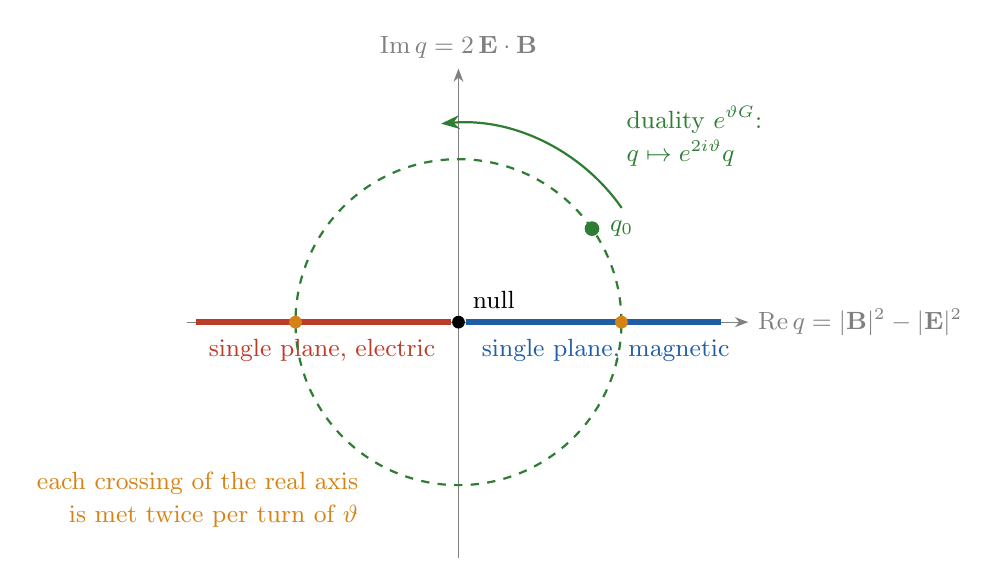
\begin{tikzpicture}[scale=1.15,>=Stealth]
\draw[->,gray] (-3.0,0) -- (3.2,0) node[right] {\small $\Re q=|\bB|^2-|\bE|^2$};
\draw[->,gray] (0,-2.6) -- (0,2.8) node[above] {\small $\Im q=2\,\bE\cdot\bB$};
\draw[scol,line width=2.2pt] (-2.9,0) -- (-0.08,0);
\draw[tcol,line width=2.2pt] (0.08,0) -- (2.9,0);
\node[tcol,anchor=north west] at (0.15,-0.08) {\small single plane, magnetic};
\node[scol,anchor=north east] at (-0.15,-0.08) {\small single plane, electric};
\fill[black] (0,0) circle (2pt);
\node[anchor=north west] at (0.05,0.45) {\small null};
\draw[gcol,thick,dashed] (0,0) circle (1.8);
\coordinate (q0) at ({1.8*cos(35)},{1.8*sin(35)});
\fill[gcol] (q0) circle (2.3pt);
\node[gcol,right=3pt] at (q0) {\small $q_0$};
\draw[->,gcol,thick] ({2.2*cos(35)},{2.2*sin(35)}) arc (35:95:2.2);
\node[gcol,align=left,anchor=west] at (1.75,2.05) {\small duality $e^{\vartheta G}$:\\ \small $q\mapsto e^{2i\vartheta}q$};
\foreach \a in {0,180}{\fill[ocol] ({1.8*cos(\a)},{1.8*sin(\a)}) circle (2.0pt);}
\node[ocol,anchor=north east,align=right] at (-1.0,-1.55) {\small each crossing of the real axis\\ \small is met twice per turn of $\vartheta$};
\end{tikzpicture}
\caption{The plane of the complex invariant $q=z\cdot z$ of a frame vector (\cref{thm:emfield,prop:planes}). The real axis is the
locus $\bE\cdot\bB=0$ on which the spacetime two-form is a single plane, magnetic on the right and electric on the left; the origin is
the null cone. A duality rotation $e^{\vartheta G}$ preserves $|q|$ and turns $q$ at twice the rate, so a non-null field becomes a single
plane four times as $\vartheta$ runs once around.}
\label{fig:qplane}
\end{figure}

Everything in this section is a statement about a representation and its invariants. \Cref{thm:twoops} is a multiplicity count that
fixes the form of the equations and nothing about their content: it does not produce a source, does not say that a source is the
current of anything, supplies no coupling constant and no Lagrangian. Nor is any of it special to this arena, since the count uses only
$\so{1,3}$ and $\Lambda^2$. What the arena adds is that the objects the count needs, the module, the duality and the invariants, were
already present, so that the system can be written in the arena's own variables \eqref{eq:RS}. The deflationary test of
\cref{sec:deflation} applies to it in full.

\section{Spin one in both readings}
\label{sec:spin}

A photon is a massless particle of spin one with two helicities. Its covariant description is a field strength, a two-form, and
its potential is a four-vector defined up to gauge. The arena offers two places for it. In the \emph{interior reading} the
potential is a grade-one element of the four-plane $E$ on which the Dirac sector is built and the field strength is the grade-two
module of \cref{prop:bivectorF}. In the \emph{frame reading} the field strength occupies the six directions themselves, under the
algebra $\lG$ of \cref{thm:GLorentz}. This section shows that each reading produces a free field with the spin content of the photon,
that the two are related by the Klein correspondence, and that at the second rung both can be housed under one Lorentz action and
coupled to a Dirac block. \Cref{fig:tworoutes} summarises the comparison.

\subsection{The univectorial photon}

\begin{proposition}[Grade one under the interior action]
\label{prop:gradeone}
Under $\lint\oplus\uu1_J$, with $J=e_2e_3$ acting by $\ad(J/2)$,
\[
V=\bigl(\tfrac12,\tfrac12\bigr)_0\oplus(0,0)_{+1}\oplus(0,0)_{-1}.
\]
The Lorentz Casimir is $\operatorname{diag}(3,0,0,3,3,3)$ on $(e_1,\dots,e_6)$, and $\ad(J/2)$ vanishes on the four-plane and acts on
$(e_2,e_3)$ by $\bigl(\begin{smallmatrix}0&1\\-1&0\end{smallmatrix}\bigr)$, with eigenvalues $\pm i$.
\end{proposition}

The potential $A=A^\mu\gamma_\mu$ is therefore neutral under the charge, as a photon must be, while the surplus pair is a Lorentz
scalar of charge $\pm1$. The photon potential is the four-plane part of grade one, not the whole of it.

\begin{proposition}[Spin one and spin one-half from the same rotors]
\label{prop:samerotors}
The interior rotations $S_k$ satisfy $[S_i,S_j]=\epsilon_{ijk}S_k$. On grade one $\ad S_k$ acts on $(e_4,e_5,e_6)$ as the standard
rotation generator $r_k$ and annihilates $e_1,e_2,e_3$, so that $-\sum_k(\ad S_k)^2=\operatorname{diag}(0,0,0,2,2,2)$ and
$\spec\ad S_3=\{\pm i,0,0,0,0\}$. On $S=\R^8$, by left multiplication, $-\sum_kS_k^2=\tfrac34\id$ and $S_3$ has eigenvalues $\pm\tfrac i2$.
Consequently $\exp(2\pi\ad S_3)=\id$ on grade one while $\exp(2\pi S_3)=-\id$ on $S$.
\end{proposition}

A vector transforms by conjugation, $A\mapsto RAR^{-1}$ with $R=e^{\theta S_3}$, and a spinor by left multiplication,
$\psi\mapsto R\psi$. At $\theta=2\pi$ the rotor is $-\id$; the sign cancels in the first case and survives in the second. This is the
space-time-algebra account of the difference between vectors and spinors \cite{Hestenes66}, realised here by the rotors of the Dirac
sector: the same $S_k$ give spin one to the potential and spin one-half to matter.

\begin{theorem}[Maxwell's equations as one Clifford equation]
\label{thm:nablaF}
Put $\nabla=\gamma^\mu\partial_\mu$ and $\sigma_k=\gamma_k\gamma_0$.
\begin{enumerate}[label=(\roman*),leftmargin=2.2em]
\item For $A=A^\mu\gamma_\mu$, $\nabla A=\partial\cdot A+\nabla\wedge A$, and for $F:=\nabla\wedge A$ the grade-one part of $\nabla F$ is
$(\Box A^\nu-\partial^\nu\partial\cdot A)\gamma_\nu$, while its grade-three part vanishes identically.
\item $F=\bE+\Omega\,\bB$ with $\bE=\sum_kE_k\sigma_k$, $E_k=-\partial_kA^0-\partial_tA^k$ and $\bB=\curl\bA$.
\item For every $F=\sum_k(E_k\sigma_k+B_k\Omega\sigma_k)$,
\[
\nabla F=(\nabla\cdot\bE)\gamma_0+(\curl\bB-\partial_t\bE)^k\gamma_k+\Omega\bigl[-(\nabla\cdot\bB)\gamma_0+(\partial_t\bB+\curl\bE)^k\gamma_k\bigr],
\]
with no other grades.
\end{enumerate}
Hence $\nabla F=\mathcal J$, with $\mathcal J=\rho\gamma_0+\mathcal J^k\gamma_k$, is Gauss's law, the Amp\`ere--Maxwell law, the absence of
magnetic charge and Faraday's law, and for $F=\nabla\wedge A$ the last two hold identically.
\end{theorem}

This is Hestenes' single Maxwell equation \cite{Hestenes66}, here on the four-plane of the Dirac sector inside the $8\times8$ matrices
of $\Cl(3,3)$. Plane waves show how the gauge freedom removes the unphysical polarisations and how helicity appears.

\begin{example}[A plane wave of the univectorial photon]
\label{ex:univectorwave}
Let $k=\gamma_0+\gamma_3$, so $k^2=0$, and $\varepsilon=\varepsilon^\mu\gamma_\mu$ with $k\cdot\varepsilon=0$, that is $\varepsilon^0=\varepsilon^3$. Then
\[
F(\varepsilon)=k\varepsilon=\varepsilon^1F_1+\varepsilon^2F_2,\qquad F_j=k\gamma_j ,
\]
because the component of $\varepsilon$ along $k$ drops out, $k^2=0$. The condition $k\cdot\varepsilon=0$ has removed the component along the
other null direction $\gamma_0-\gamma_3$, so only the two transverse polarisations remain, and the gauge freedom
$\varepsilon\mapsto\varepsilon+ck$ is exactly the helicity-zero direction. Moreover $F_j^2=0$ and $F_1F_2+F_2F_1=0$, so every $F(\varepsilon)$ squares
to zero: in the space-time algebra $F^2=\bE^2-\bB^2+2\Omega\,\bE\cdot\bB$, so this is the null condition $|\bE|=|\bB|$,
$\bE\perp\bB$. On $\operatorname{span}\{F_1,F_2\}$,
\[
\ad S_3=\begin{pmatrix}0&-1\\1&0\end{pmatrix},\qquad \Omega=\begin{pmatrix}0&1\\-1&0\end{pmatrix}=-\ad S_3 ,
\]
both with eigenvalues $\pm i$. For positive-frequency waves the eigenvectors of $\ad S_3$ with eigenvalues $\mp i$ carry helicity
$\pm1$, and on them the Hodge star is $i$ times the helicity: circular polarisation is self-duality or anti-self-duality of $F$.
\end{example}

\begin{proposition}[Every field-strength module under the interior action]
\label{prop:censusint}
The Lorentz Casimir on the grades of $\Cl(3,3)$, the number of field-strength modules (Casimir value $4$) and their charges under
$\ad(J/2)$ are
\begin{center}
\begin{tabular}{@{}clcc@{}}
\toprule
grade & spectrum of the Casimir (multiplicity) & field-strength modules & charges\\
\midrule
$0,6$ & $0\,(1)$ & $0$ & ---\\
$1,5$ & $3\,(4)$, $0\,(2)$ & $0$ & ---\\
$2,4$ & $4\,(6)$, $3\,(8)$, $0\,(1)$ & $1$ & $0$\\
$3$ & $4\,(12)$, $3\,(8)$ & $2$ & $\pm1$\\
\bottomrule
\end{tabular}
\end{center}
and on $S$ the Casimir is $\tfrac32$ throughout.
\end{proposition}

Because $J$ commutes with the four-plane, the grade-four module is $J$ times the grade-two one, and $J$ is the complex structure at
one constituent (\cref{thm:i}). Up to that complex structure the neutral field strength is unique and sits at grade two; the two
grade-three copies carry charge $\pm1$ and are not candidates for the photon.

\subsection{The frame photon}

In the frame reading the field strength is the vector $X$ itself, and the boosts of $\lG$ turn out to be the spin matrices of the
photon.

\begin{proposition}[Spin matrices on the frame]
\label{prop:spinmatrices}
$K_k=GL_k$ for $k=1,2,3$, both families commute with $G$ and preserve $\eta$, and the Casimir $\sum K_k^2-\sum L_k^2$ equals $4\,\id$ on
$V$, the field-strength value. On $z=\bB+i\bE$ the rotation $L_k$ acts as $r_k$ and the boost $K_k$ as
\[
s_k=i\,r_k,\qquad (s_k)_{ab}=-i\epsilon_{kab},
\]
which are Hermitian with $[s_i,s_j]=i\epsilon_{ijk}s_k$, $\sum_ks_k^2=2\,\id$ and $\spec s_3=\{-1,0,1\}$. With $p=-i\nabla$ one has
$(s\cdot p)z=\curl z$ identically, so the frame Maxwell system \eqref{eq:RS} is the photon wave equation
\[
i\partial_tz=(s\cdot p)\,z,\qquad p\cdot z=0 ,
\]
and the kernel of $s_3$ is spanned by $\hat e_3$: transversality removes exactly the helicity-zero component of a wave moving along
$\hat e_3$.
\end{proposition}

These are the spin-one matrices that Oppenheimer and Bialynicki-Birula use to write the photon wave function
\cite{Oppenheimer1931,BialynickiBirula96}. The rotations act on $z$ as $r_k$, and their Hermitian generators $s_k=ir_k$ are the action
of the boosts, because on this module a boost is $G$ times a rotation.

\begin{proposition}[Orthogonality on the frame]
\label{prop:orthframe}
For $X=\sum_i(B_ie_i+E_ie_{i+3})$,
\[
z\cdot z=\eta(X,X)-i\,\eta(X,GX).
\]
Hence $\bE\perp\bB$ exactly when $X\perp_\eta GX$, $|\bE|=|\bB|$ exactly when $X$ is $\eta$-null, and both hold exactly when the plane
$\operatorname{span}\{X,GX\}$ is totally $\eta$-null.
\end{proposition}

\begin{theorem}[The axis of a null field]
\label{thm:axis}
For real $a,b\in\R^3$,
\[
\bigl(s\cdot(a\times b)\bigr)(a+ib)=|b|^2a+i|a|^2b-(a\cdot b)(b+ia).
\]
Consequently a nonzero $z=\bB+i\bE$ satisfies $z\cdot z=0$ if and only if $(s\cdot n)z=z$ for some real unit vector $n$, and then
$n=\bB\times\bE/|\bB\times\bE|$ uniquely.
\end{theorem}

\begin{proof}
If $z\cdot z=0$ then $\bB\cdot\bE=0$ and $|\bB|=|\bE|\neq0$; the identity gives $(s\cdot(\bB\times\bE))z=|\bB|^2z$ and
$|\bB\times\bE|=|\bB|^2$. Conversely $n\cdot((s\cdot n)z)=0$ and $z\cdot((s\cdot n)z)=0$ identically, and the characteristic polynomial
of $s\cdot n$ is $-\lambda(\lambda^2-|n|^2)$, so the eigenvalue $1$ forces $n\cdot z=0$ and $z\cdot z=0$. For uniqueness,
$(s\cdot n)z=in\times z=z$ splits into $\bB=-n\times\bE$ and $\bE=n\times\bB$, whence $n\perp\bB$ and $\bB\times\bE=|\bB|^2n$.
\end{proof}

Since $\bB\times\bE=\bE\times\Btext$ is the Poynting vector, a null field is the $m=+1$ state of the photon spin along its own energy
flux, the frame form of the classical fact that a null field determines a unique direction of propagation
\cite{Synge56,Robinson61}. Orthogonality with equal magnitudes therefore singles out the null fields and their axis. It does not
single out a helicity.

\begin{example}[Three null waves with one axis]
\label{ex:threewaves}
The fields
\[
z_\pm=(1,i,0)\,e^{\pm ik(x_3-t)},\qquad z_{\rm lin}=(1,i,0)\cos k(x_3-t)
\]
all solve \eqref{eq:RS}. In each, $\bB\cdot\bE=0$, $|\bB|=|\bE|$ and $\bB\times\bE$ points along $+\hat e_3$ wherever $z\neq0$, so each is an
$m=+1$ state along $\hat e_3$. At $x_3=0$ the electric field turns according to $(\bE\times\dot\bE)\cdot\hat e_3=+k,\,-k,\,0$: helicity
$+1$, helicity $-1$, and a linear superposition. The difference is the sign of the frequency, $z_+\propto e^{-ikt}$ against
$z_-\propto e^{+ikt}$, which is the Bialynicki-Birula assignment for the Riemann--Silberstein vector \cite{BialynickiBirula96}. Not every
radiation field is null either: $z=(1,i,0)\cos k(x_3-t)+(0,1,i)\cos k(x_1-t)$ solves the system and has $|\bB|=|\bE|$, but
$\bB\cdot\bE=\cos k(x_1-t)\cos k(x_3-t)$.
\end{example}

Orthogonality alone is weaker still. The field $X=(\bB;\bE)=(1,0,0;\,0,2,0)$ has $\eta(X,GX)=0$, so $\bE\perp\bB$, but
$\eta(X,X)=1-4=-3$; the boost $e^{\theta K_3}$ with $\theta=-\tfrac12\log3$ carries it to $(0,0,0;\,0,\sqrt3,0)$, a purely electric field
with the same invariant. A field with $\bE\perp\bB$ and $|\bE|\neq|\bB|$ is purely electric or purely magnetic in a suitable frame
\cite{LandauLifshitz2}. On the null line $\C(1,i,0)$, by contrast, $e^{\theta K_3}$ acts by multiplication by $e^\theta$; with
$\theta=-\operatorname{artanh}\beta$ for a frame moving with velocity $\beta\hat e_3$ this is the Doppler factor $\sqrt{(1-\beta)/(1+\beta)}$.
The stabiliser of the axis acts on a null field by the helicity phase and by the Doppler factor.

\subsection{Potentials on the frame, and helicity as a charge}
\label{sec:potentials}

Place a vector potential on each triple, $\bA$ on $e_1,e_2,e_3$ and $\mathbf C$ on $e_4,e_5,e_6$, write $X_A=(\bA;\mathbf C)$ and
$X_F=\curl X_A$, the curl acting on each triple, and take
\begin{equation}
\label{eq:SSL}
\mathcal L=\tfrac12\,(\curl X_A)\cdot G\dot X_A-\tfrac12\,|\curl X_A|^2
\end{equation}
with the Euclidean dot product of $\R^6$, for which $G$ is orthogonal.

\begin{theorem}[Duality-symmetric Maxwell theory on the frame]
\label{thm:SS}
\begin{enumerate}[label=(\roman*),leftmargin=2.2em]
\item The Euler--Lagrange expression of \eqref{eq:SSL} is $G\curl\bigl(\dot X_A+G\curl X_A\bigr)$. Every solution of the first-order
equation $\dot X_A=-G\curl X_A$ solves it, and on a contractible region every solution satisfies the first-order equation up to a
time-dependent gauge transformation.
\item On solutions, $X_F$ obeys the frame Maxwell system \eqref{eq:RS} with $\bB=\curl\bA$ and $\bE=\curl\mathbf C$.
\item Under $X_A\mapsto X_A+(\nabla\lambda_1;\nabla\lambda_2)$, $X_F$ is unchanged and $\mathcal L$ changes by a divergence.
\item The Hamiltonian is $\tfrac12|\curl X_A|^2=\tfrac12(|\bB|^2+|\bE|^2)$, the energy density.
\item $\mathcal L(e^{\theta G}X_A)=\mathcal L(X_A)$ exactly, and the Noether current of $\delta X_A=GX_A$ has density
$j^0=-\tfrac12X_A\cdot\curl X_A$. For fields that decay or are periodic the conserved charge is $-\mathcal K$, where
\[
\mathcal K=\tfrac12\int X_A\cdot\curl X_A\,d^3x=\tfrac12\int(\bA\cdot\bB+\mathbf C\cdot\bE)\,d^3x
\]
is the optical helicity.
\end{enumerate}
\end{theorem}

This is the duality-symmetric first-order formulation of Schwarz and Sen \cite{SchwarzSen94}, with two vector potentials in the
temporal gauge and with the binding root $G$ in the place of their $SO(2)$ generator; the conserved charge of the duality rotation is,
up to sign, the optical helicity \cite{Calkin65,DeserTeitelboim76,CameronBarnettYao12}.

\begin{example}[The $G$-charge is the helicity]
\label{ex:Gcharge}
For waves $e^{i(k x_3-\omega t)}$ the first-order equation reads $\omega a=G(k\times a)$, a $6\times6$ matrix with eigenvalues $\pm k$, each
twice, and $0$ twice (the longitudinal, pure-gauge pair). The eigenspace $\omega=+k$ is spanned by
\[
\begin{aligned}
a_1&=(1,-i)\otimes(1,i,0), & Ga_1&=ia_1, & s_3a_1&=a_1,\\
a_2&=(1,i)\otimes(1,-i,0), & Ga_2&=-ia_2, & s_3a_2&=-a_2,
\end{aligned}
\]
with $s_3$ acting on each triple. For the real waves $X_A=\Re(a\,e^{ik(x_3-t)})$ the helicity density $\tfrac12X_A\cdot\curl X_A$ and the
energy density are $(k,k^2)$ for $a_1$, $(-k,k^2)$ for $a_2$, and $(0,4k^2\sin^2k(x_3-t))$ for $a_1+a_2$. On positive-frequency modes the
eigenvalue of $G$ is $i$ times the helicity. The ratio of helicity to energy is $\pm1/\omega$, which for a quantised field of energy
$N\hbar\omega$ is $\pm N\hbar$: one unit of $\hbar$ per photon, the spin-one value.
\end{example}

The frame potentials are not components of a Lorentz tensor. Neither the constant boost $\delta X_A=K_3X_A$ nor the boost of the
coordinates is a symmetry of \eqref{eq:SSL}; the boost that is one is the Schwarz--Sen transformation $\delta X_A=t\,\partial_3X_A-x_3\,G\curl
X_A$, whose curl is, identically,
\[
\curl\bigl(t\,\partial_3X_A-x_3\,G\curl X_A\bigr)=t\,\partial_3X_F-x_3\,G\curl X_F-K_3X_F ,
\]
which on solutions is the boost of the field strength along $\hat e_3$ with its orbital part and its spin part $K_3$. Boosts reach the
potentials only through their curl and only on shell \cite{SchwarzSen94}. Duality rotations, for their part, are not Lorentz
transformations: $e^{\theta G}$ preserves the energy density and rotates $\eta(X,X)$ into $\eta(X,GX)$.

\subsection{The bridge between the readings}
\label{sec:bridge}

\begin{proposition}[Half-spinors under the two algebras]
\label{prop:halfspinors}
Under $\lint$ the Casimir on $S^\pm$ is $\tfrac32$, and $S^+$ carries a two-parameter family of invariant antisymmetric forms and no
invariant symmetric one: it is a Weyl module. Under $\lG$ the Casimir on all of $S$ is $3$, the invariant symmetric forms on $S^+$ form a
one-parameter family of Lorentzian forms, and there is no invariant antisymmetric form: $S^+$ is a Minkowski four-vector, and
$\exp(2\pi L_3)=+\id$ on $S$. On $\C^8$ the two algebras give $2\,(\tfrac12,0)\oplus2\,(0,\tfrac12)$ and $2\,(\tfrac12,\tfrac12)$
respectively, and they meet in zero.
\end{proposition}

So under the binding algebra every spinor of $\Cl(3,3)$ has integer spin, in accordance with $\mathrm{Spin}(3,3)\cong SL(4,\R)$, whose
half-spinor modules are $\R^4$ and its dual \cite{Porteous}. This sharpens \cref{prop:emexclusive}: with $\lG$ as the Lorentz algebra
one constituent carries no spin one-half at all.

\begin{theorem}[The Klein correspondence]
\label{thm:klein}
The $\mathrm{Spin}(3,3)$-invariant bilinear forms on $S$ form a two-dimensional space. For one of them, $\beta$, the map
$W(X)(\psi,\chi)=\beta(\psi,X\chi)$ on $S^+$ is antisymmetric and equivariant, and
\[
\Pf W(X)=\eta(X,X).
\]
Hence $V\cong\Lambda^2(S^+)^*$ as $\mathrm{Spin}(3,3)$-modules, and the null cone of $\eta$ is the set of decomposable two-forms.
\end{theorem}

This is the Klein correspondence between the points of the Klein quadric and the lines of projective three-space
\cite{WardWells}. It can be compared with the frame reading. Let $T:\R^{1,3}\to S^+$ be the $\lG$-intertwiner, unique up to scale. Then
\[
T^*W(X)=-F_X+\star F_X=\sqrt2\,F_{e^{3\pi G/4}X}\qquad\text{for all }X,
\]
so the canonical identification of $V$ with two-forms on the half-spinor and the frame reading of the field strength differ by a
duality rotation of an eighth of a turn, $-\pi/4$ modulo $\pi$. In the Klein frame $\eta(X,X)$ is the Pfaffian, the invariant of
$\bE\cdot\bB$ type, and $\eta(X,GX)$ the Hodge pairing; in the frame reading the roles are the other way round. For free fields the two
readings are equivalent, since duality rotations map solutions to solutions; a statement that singles out one invariant, such as which
of them is the Lagrangian, holds in one reading and not in the other. A plane wave $\kappa\wedge\alpha$ built on $S^+$, with $\kappa$ the
lowered null momentum $(1,0,0,1)$ and $\alpha$ the polarisation $(0,1,0,0)$, lands on the doubly null vector
$X=(-\tfrac12,-\tfrac12,0;\,\tfrac12,-\tfrac12,0)$, whose Poynting axis $\bB\times\bE=(0,0,\tfrac12)$ is the spatial momentum; the Klein
planes of $X$ and of $GX$ meet in the null line $[\kappa]$, as two lines of projective space joined by a line of the quadric must.

\begin{figure}[t]
\centering
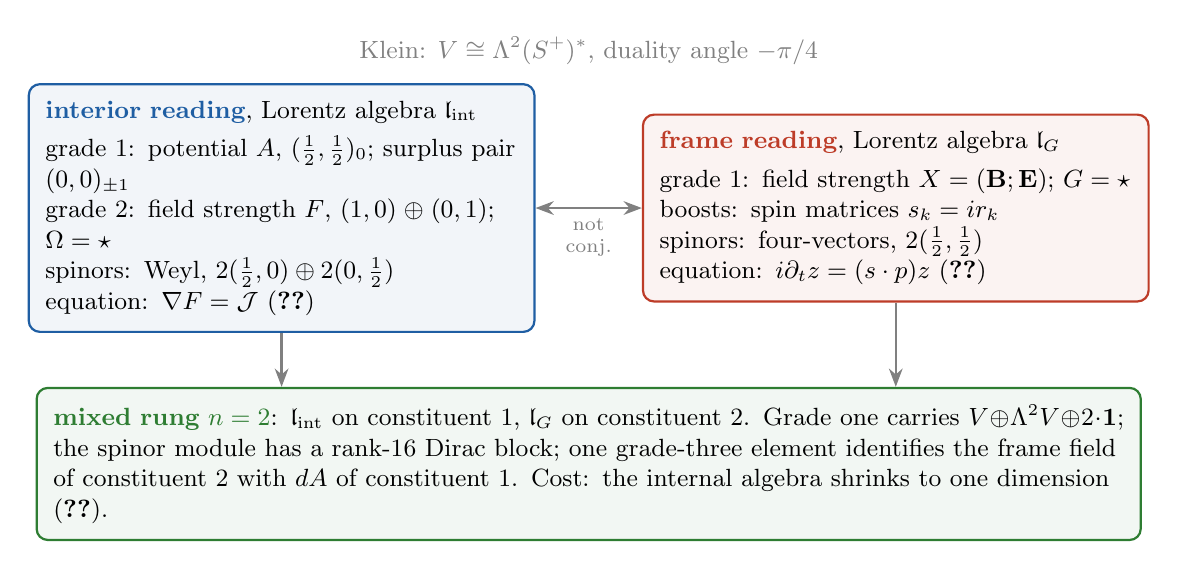
\begin{tikzpicture}[>=Stealth,font=\small]
\node[draw=tcol,thick,rounded corners=4pt,fill=tcol!6,text width=6.0cm,align=left,inner sep=6pt] (int) at (0,0) {%
\textbf{\textcolor{tcol}{interior reading}}, Lorentz algebra $\lint$\\[3pt]
grade 1: potential $A$, $(\tfrac12,\tfrac12)_0$; surplus pair $(0,0)_{\pm1}$\\
grade 2: field strength $F$, $(1,0)\oplus(0,1)$; $\Omega=\star$\\
spinors: Weyl, $2(\tfrac12,0)\oplus2(0,\tfrac12)$\\
equation: $\nabla F=\mathcal J$ (\cref{thm:nablaF})};
\node[draw=scol,thick,rounded corners=4pt,fill=scol!6,text width=6.0cm,align=left,inner sep=6pt] (bin) at (7.8,0) {%
\textbf{\textcolor{scol}{frame reading}}, Lorentz algebra $\lG$\\[3pt]
grade 1: field strength $X=(\bB;\bE)$; $G=\star$\\
boosts: spin matrices $s_k=ir_k$\\
spinors: four-vectors, $2(\tfrac12,\tfrac12)$\\
equation: $i\partial_tz=(s\cdot p)z$ (\cref{prop:spinmatrices})};
\draw[<->,thick,gray] (int.east) -- node[below,align=center,font=\scriptsize] {not\\ conj.} (bin.west);
\node[draw=gcol,thick,rounded corners=4pt,fill=gcol!6,text width=13.6cm,align=left,inner sep=6pt] (mix) at (3.9,-3.25) {%
\textbf{\textcolor{gcol}{mixed rung $n=2$}}: $\lint$ on constituent 1, $\lG$ on constituent 2. Grade one carries
$V\oplus\Lambda^2V\oplus2\cdot\mathbf1$; the spinor module has a rank-$16$ Dirac block; one grade-three element identifies the
frame field of constituent 2 with $dA$ of constituent 1. Cost: the internal algebra shrinks to one dimension
(\cref{prop:mixedcost}).};
\draw[->,thick,gray] (int.south) -- (int.south |- mix.north);
\draw[->,thick,gray] (bin.south) -- (bin.south |- mix.north);
\node[gray,anchor=south] at (3.9,1.7) {Klein: $V\cong\Lambda^2(S^+)^*$, duality angle $-\pi/4$};
\end{tikzpicture}
\caption{Two places for the photon in the arena (\cref{sec:spin}). Each reading gives a free field with the spin content of the photon;
on one constituent they use non-conjugate Lorentz algebras and do not merge, and at the second rung they can be housed together at
the price of the internal algebra.}
\label{fig:tworoutes}
\end{figure}

\subsection{The tower}

On the tower the two readings multiply in different ways.

\begin{proposition}[Commutants along the tower]
\label{prop:commutantsn}
On $V_n=\R^{3n,3n}$ the commutants have the following dimensions:
\begin{center}
\begin{tabular}{@{}lccccc@{}}
\toprule
commutant of & $n=1$ & $2$ & $3$ & $4$ & $5$\\
\midrule
spectator $\lint$ in $\so{3n,3n}$ & $1$ & $28$ & $91$ & $190$ & $325$\\
diagonal $\lint$ in $\so{3n,3n}$ & $1$ & $7$ & $18$ & $34$ & $55$\\
diagonal $\lG$ in $\so{3n,3n}$ & $0$ & $2$ & $6$ & $12$ & $20$\\
diagonal rotations and $G_n$ in $\so{6n}$ & $1$ & $4$ & $9$ & $16$ & $25$\\
the same inside $\so{3n,3n}$ & $0$ & $1$ & $3$ & $6$ & $10$\\
\bottomrule
\end{tabular}
\end{center}
These are the dimensions of $\so{3n-1,3n-3}$, $\so n\oplus\so{2n}$, $\so{n,\C}$, $\uu n$ and $\so n$.
\end{proposition}

Under the diagonal interior action $V_n=n\,(\tfrac12,\tfrac12)\oplus2n\,(0,0)$, so there are $n$ potentials forming the vector of the copy
algebra $\so n$, and none of them is copy-invariant at grade one for $n\ge2$. A single univectorial potential in the diagonal sector
therefore needs a choice of direction in copy space, and any such choice breaks $\so n$ to $\so{n-1}$. The obstruction belongs to grade
one only.

\begin{theorem}[Copy-invariant four-vectors]
\label{thm:copyparity}
A copy-invariant four-vector in $\Lambda^g(\R^n\otimes\R^{1,3})$ requires $n$ odd and $g$ odd with $n\le g\le3n$, and for every odd $n$
there is one at $g=n$,
\[
Q^{(n)}_b=\epsilon_{k_1\cdots k_n}\,\eta^{a_1a_2}\cdots\eta^{a_{n-2}a_{n-1}}\,\gamma^{(k_1)}_{a_1}\wedge\cdots\wedge\gamma^{(k_{n-1})}_{a_{n-1}}\wedge\gamma^{(k_n)}_b .
\]
At $n=3$ there is exactly one at each of the grades $3,5,7,9$, and at $n=2$ there is none at any grade.
\end{theorem}

\begin{proof}
An invariant element of $\Lambda^g(\R^n\otimes\R^{1,3})\otimes\R^{1,3}$ is an invariant tensor of $SO(n)\times SO^+(1,3)$ in
$(\R^n)^{\otimes g}\otimes(\R^{1,3})^{\otimes(g+1)}$. By the first fundamental theorem for the special orthogonal groups \cite{Weyl39},
such tensors are spanned by products of metrics and at most one Levi-Civita symbol. On the Lorentz side every factor has an even number
of indices, so $g+1$ is even. On the copy side $g=2d+ne$ with $e\in\{0,1\}$; $g$ odd forces $e=1$ and $n$ odd, so $g\ge n$. The Hodge
star of $\R^n\otimes\R^{1,3}$ is an equivariant isomorphism $\Lambda^g\cong\Lambda^{4n-g}$, which gives $g\le3n$. The displayed
$Q^{(n)}_b$ is invariant because $\epsilon$ is, and nonzero because the terms of $Q^{(n)}_0$ with all Lorentz indices equal to $0$
add up to $n!\,\gamma^{(1)}_0\wedge\cdots\wedge\gamma^{(n)}_0$.
\end{proof}

At $n=3$ the invariant four-vector of grade three is, up to a factor, the copy-singlet cubic $Q_\mu$ that builds the gamma matrices of
the Dirac block in \cref{thm:blockgamma}; the parity theorem explains why such an object exists at three constituents and could not
exist at two. Under the diagonal $\lG$, finally, $V_n=n\bigl[(1,0)\oplus(0,1)\bigr]$: $n$ field strengths mixed by the complex orthogonal
flavour algebra $\so{n,\C}$. The energy-preserving duality group of $n$ free Maxwell fields is $U(n)$, the maximal compact subgroup of
the Gaillard--Zumino group $Sp(2n,\R)$ \cite{GaillardZumino81}; its Lie algebra meets $\so{3n,3n}$ only in $\so n$, and its centre,
generated by $G_n$ and carrying the total helicity, lies outside $\so{3n,3n}$, as $G$ does at $n=1$. A single photon would be one
direction in this flavour space, and nothing selects one.

\subsection{The mixed rung}
\label{sec:mixed}

\Cref{prop:emexclusive} forbids reading one six-dimensional space in two ways. At $n\ge2$ there is more than one constituent, and the
obvious repair is to let one constituent carry the interior reading and another the frame reading, under one Lorentz action.

\begin{proposition}[The mixed embedding]
\label{prop:mixed}
In $\Cl(6,6)$ let $\mathfrak l_{\rm mix}$ be spanned by $S_k\otimes1+1\otimes L_k$ and $T_k\otimes1+1\otimes K_k$: the interior algebra on
constituent $1$ and $\lG$ on constituent $2$, paired generator by generator. It satisfies the $\so{1,3}$ brackets, and
\[
\R^{6,6}=\underbrace{V}_{C=3}\oplus\underbrace{\Lambda^2V}_{C=4}\oplus2\cdot\mathbf1 ,
\]
so one Lorentz action carries both a four-vector and a field strength at grade one. On $S_2=\R^{64}$ the Casimir satisfies
$(C_{\rm mix}-\tfrac32)(C_{\rm mix}-\tfrac{11}2)=0$, with the Dirac value $\tfrac32$ on sixteen dimensions and $\tfrac{11}2$ on $48$.
\end{proposition}

\begin{proposition}[The cost]
\label{prop:mixedcost}
The centraliser of $\mathfrak l_{\rm mix}$ in $\so{6,6}$ is one-dimensional, spanned by the rotation of the surplus pair of
constituent $1$. At the same rung:
\begin{center}
\begin{tabular}{@{}lcl@{}}
\toprule
Lorentz action at $n=2$ & centraliser & content of $\R^{6,6}$\\
\midrule
interior on one constituent & $28$ & $V\oplus8\cdot\mathbf1$\\
$\lG$ on one constituent & $15$ & $\Lambda^2V\oplus6\cdot\mathbf1$\\
mixed, across both & $1$ & $V\oplus\Lambda^2V\oplus2\cdot\mathbf1$\\
\bottomrule
\end{tabular}
\end{center}
The mixed embedding buys the field-strength module at the price of the whole internal algebra: $\so{5,3}$ collapses to one $\uu1$.
\end{proposition}

The count is for this pairing of the two Lorentz bases at $n=2$; another pairing or a higher rung could do better and has not been
examined. Within its scope, however, the mixed rung is an honest place to test whether the two readings can be coupled, and it turns out
that they can.

\begin{theorem}[The Dirac block of the mixed rung]
\label{thm:mixeddirac}
Let $P=\tfrac18(11\,\id-2C_{\rm mix})$ and $\hat\gamma_\mu=2P\gamma^{(1)}_\mu P$, with $J_1=e_2e_3\otimes1$.
\begin{enumerate}[label=(\roman*),leftmargin=2.2em]
\item $P$ is the orthogonal projector of rank $16$ onto the block with the Dirac value, and commutes with the mixed generators.
\item $\{\hat\gamma_\mu,\hat\gamma_\nu\}=2\eta_{\mu\nu}P$, $[\hat\gamma_\mu,J_1]=0$, $J_1^2=-\id$, and $P\mathcal S_kP=\tfrac12\hat\gamma_i\hat\gamma_j$ (cyclic),
$P\mathcal T_kP=\tfrac12\hat\gamma_0\hat\gamma_k$: the compressed gammas generate the mixed Lorentz action on the block.
\item With $J_1$ as the imaginary unit the block is two complex Dirac modules, labelled by the half-spinors of constituent $2$, with
flavour algebra $\uu2$; $\mathcal H(p)=\hat\gamma^0\hat\gamma^ap_a+m\hat\gamma^0$ is symmetric and $\mathcal H(p)^2=(|p|^2+m^2)P$.
\item The block is the $\gamma$-trace part $\sum_a\gamma_a\chi\otimes\tau e_a$ of the vector-spinors (Dirac spinor of constituent $1$)
$\otimes$(four-vector of constituent $2$), and the rank-$48$ block is their $\gamma$-traceless $(1,\tfrac12)\oplus(\tfrac12,1)$ part.
\end{enumerate}
\end{theorem}

Item (iv) explains the factor $2$ in $\hat\gamma_\mu$, since $P\gamma^{(1)}_\mu$ acts on the $\gamma$-trace part as $-\tfrac12\gamma_\mu$, and it
identifies the decomposition with the classical splitting of a vector-spinor into its trace and its traceless part
\cite{RaritaSchwinger41}.

A covariant identification of the field strength of constituent $1$ with the frame field of constituent $2$ is an invariant element
of $\Lambda^2(\text{four-plane}_1)\otimes V_2$, that is, a grade-three element of the algebra commuting with the mixed generators. The
invariant space is two-dimensional, and one invariant is
\[
\Theta_F=\gamma^{(1)}_2\gamma^{(1)}_3e'_1+\gamma^{(1)}_3\gamma^{(1)}_1e'_2+\gamma^{(1)}_1\gamma^{(1)}_2e'_3
-\gamma^{(1)}_0\gamma^{(1)}_1e'_4-\gamma^{(1)}_0\gamma^{(1)}_2e'_5-\gamma^{(1)}_0\gamma^{(1)}_3e'_6 ,
\]
with $e'_a$ the generators of constituent $2$; it pairs the spatial bivectors of constituent $1$ with the magnetic directions of
constituent $2$ and the time--space bivectors with the electric ones. The other invariant is $\Theta_F$ followed by $G$, so up to scale
the identifications form the family $X=e^{\theta G}X_F$.

\begin{theorem}[A coupled model]
\label{thm:coupled}
On the block, in flavour coordinates $\R^8\otimes\R^2$ with $\hat\gamma_\mu=-\gamma_\mu\otimes1$, $J_1=J\otimes1$ and $U^\mu=\hat\gamma^0\hat\gamma^\mu$, take
for commuting real fields
\begin{equation}
\label{eq:coupledL}
\mathcal L=-\tfrac14F_{\mu\nu}F^{\mu\nu}+\psi^{\!\top}J_1U^\mu D_\mu\psi-m\,\psi^{\!\top}\hat\gamma^0\psi,\qquad D_\mu=\partial_\mu+qA_\mu J_1 ,
\end{equation}
the real form of $-\tfrac14F^2+\bar\psi(i\gamma^\mu D_\mu-m)\psi$ with $J_1$ in the place of $i$. Then the field equations are Maxwell's
equations $\partial_\mu F^{\mu\nu}=q\,j^\nu$ with $j^\nu=\psi^{\!\top}U^\nu\psi$ and $j^0=|\psi|^2$, and the Dirac equation
$J_1\hat\gamma^\mu D_\mu\psi=m\psi$; the identity $\partial_\mu j^\mu+\psi^{\!\top}J_1\mathcal E_\psi=0$ holds with $\mathcal E_\psi$ the Dirac
expression; the Lagrangian is exactly invariant under $\psi\mapsto e^{-q\lambda J_1}\psi$, $A\mapsto A+\partial\lambda$; and its flavour
symmetry is the $\uu2$ spanned by $J\otimes1$, $1\otimes\epsilon$, $J\otimes\sigma_x$, $J\otimes\sigma_z$. The potential carries two
polarisations of helicity $\pm1$ and no massive mode, and each momentum carries two flavours, two helicities and two signs of frequency.
\end{theorem}

In the frame reading the source is electric. For the frame field of an arbitrary potential one has, identically,
$\partial_tz+i\curl z+i\boldsymbol{\mathcal J}=0$ and $\nabla\cdot z=i\rho$ with $(\rho,\boldsymbol{\mathcal J})=\partial_\mu F^{\mu\nu}$, and the
rotated field $e^{\theta G}X_F$ satisfies the same system with electric source $\cos\theta$ times the current and magnetic source $\sin\theta$
times it. Since the frame field takes no part in the dynamics of \eqref{eq:coupledL}, which member of the family is called the frame
field is a choice; requiring it to carry electric sources only fixes $\theta\equiv0$ modulo $\pi$, as in the textbook treatment of duality
with sources, where the angle is fixed by the convention that all charges are electric \cite{Jackson}. The duality rotation, a symmetry
of the free system and of \eqref{eq:SSL}, is not a symmetry once electric sources are present.

The coupled model is classical two-flavour spinor electrodynamics with equal charges, written in the algebra of the second rung. It
is a construction, not a selection, and it has a definite limitation that we record now and use later: the second-rung vacuum of
\cref{sec:photon} is defined for the spectator action, and under the mixed action it is preserved only by the rotations about one axis,
so the coupled model lies outside that vacuum sector.

At even rungs, finally, the diagonal interior action places integer-spin modules inside the spinor module itself: at $n=2$ the Casimir
takes the values $0,3,4$ on $8,32,24$ dimensions, so $S_2$ contains scalars of copy charge $\pm2$, four-vectors of copy charge $\pm1$ and
copy-neutral field strengths $(1,0)\oplus(0,1)$, and the copy and Lorentz Casimirs add up to $4$, the $n=2$ case of \eqref{eq:casid}. These
are modules of one spinor space, not bound states, and we do not propose them as the photon.

\section{The orthogonality of the electric and magnetic fields}
\label{sec:orth}

In the frame reading the orthogonality of $\bE$ and $\bB$ is the reality of the complex invariant, $\Im q=2\,\bE\cdot\bB=0$, and
by \cref{prop:planes} it is also the condition for the spacetime two-form to be a single plane. Since the arena puts $\bE$ and $\bB$
on two orthogonal triples, it is natural to ask what orthogonality means physically: what breaks it, whether its failure is a
symmetry breaking, and whether it can produce mass. The answers are classical once the right questions are asked, and they come out
sharply negative on the last point.

\subsection{What orthogonality is}

The field strength $F^\mu{}_\nu$ has eigenvalues $\pm\epsilon_E$ and $\pm i\epsilon_M$ with
\[
\epsilon_E=|\Im\sqrt q|,\qquad \epsilon_M=|\Re\sqrt q|,
\]
and $\bE\cdot\bB=\Pf F=0$ exactly when $F$ is one plane: a pure boost, a pure rotation or a null rotation. Otherwise $F$ generates a
screw, a boost and a rotation about a common axis. Two simple facts locate orthogonality among all fields.

\begin{proposition}[Single modes are orthogonal]
\label{prop:modes}
Let $F=k\wedge b$ with $k,b$ real four-vectors. Then $\Pf F=0$ and $q=(k\cdot k)(b\cdot b)-(k\cdot b)^2$ is real. The field of a mode
$A_\mu=\Re(a_\mu e^{-ik\cdot x})$ with real $k$ and $k\cdot a=0$ is $k\wedge b(x)$ with $k\cdot b=0$, for every polarisation. A Maxwell mode,
$k\cdot k=0$, is therefore null at every point, and a Proca mode, $k\cdot k=m^2$, has $q=m^2(b\cdot b)\le0$: it is orthogonal and of
electric type everywhere.
\end{proposition}

A mass does not show in the angle between the fields of a single mode; it shows in the other invariant, which it makes nonzero.
The null cone $q=0$ is the massless locus, and orthogonality is a much larger set, containing every single mode of every mass.

\begin{proposition}[Superposition breaks it]
\label{prop:twomodes}
$\Pf(k_1\wedge b_1+k_2\wedge b_2)=\det(k_1^\flat,b_1^\flat,k_2^\flat,b_2^\flat)$. At a point, two modes give $\bE\cdot\bB\neq0$ exactly when
their two planes together span spacetime. Waves propagating along one null direction $\ell$ never do: the total field is
$\ell\wedge\sum_j\omega_jb_j$, a single null plane.
\end{proposition}

\begin{example}[Counter-propagating waves]
\label{ex:counter}
In textbook variables, with $\omega=k$, let a wave along $+z$ polarised along $x$ meet a wave along $-z$. With crossed polarisations,
$\bE=(\cos(kz-kt),\cos(kz+kt),0)$ and $\Btext=(\cos(kz+kt),\cos(kz-kt),0)$; with parallel ones,
$\bE=(\cos(kz-kt)+\cos(kz+kt),0,0)$ and $\Btext=(0,\cos(kz-kt)-\cos(kz+kt),0)$. Both solve Maxwell's equations, and
\[
\begin{aligned}
&\text{crossed:}&& \bE\cdot\Btext=\cos2kz+\cos2kt, && |\Btext|^2-|\bE|^2=0,\\
&\text{parallel:}&& \bE\cdot\Btext=0, && |\Btext|^2-|\bE|^2=-2(\cos2kz+\cos2kt).
\end{aligned}
\]
The two configurations have the same energy density and the same Poynting vector at every point. The reason is structural: the crossed
configuration is the parallel one turned by $\pi/4$ about the $z$ axis and then duality-rotated by $\pi/4$; the rotation preserves the
energy density and the Poynting vector along $z$, the duality rotation preserves the entire energy--momentum tensor, and only the phase
of $q$ moves.
\end{example}

Nothing exotic is needed to break orthogonality. Near the ground the fair-weather electric field of the atmosphere, about $100$~V/m
and vertical \cite{FeynmanII}, meets the geomagnetic field, which is inclined to the horizontal everywhere except on the magnetic
equator.

\subsection{How it changes in time}

\begin{proposition}[The local law]
\label{prop:EBlocal}
With $\partial_t\bB=\curl\bE$ and $\partial_t\bE=-\curl\bB-\bj$,
\[
\partial_tq=-2i\,z\cdot(\curl z)-2i\,z\cdot\bj,\qquad \partial_t(\bE\cdot\bB)=\bE\cdot\curl\bE-\bB\cdot\curl\bB-\bj\cdot\bB ,
\]
in textbook variables $\partial_t(\bE\cdot\Btext)=\Btext\cdot\curl\Btext-\bE\cdot\curl\bE-\bj\cdot\Btext$. With potentials,
$\Btext=\curl\bA$, $\bE=-\partial_t\bA-\nabla\phi$, and in a source-free region $\bE=-\curl\mathbf C$, $\Btext=-\partial_t\mathbf C+\nabla\chi$,
\[
\partial_t(\bA\cdot\Btext)+\nabla\cdot(\phi\Btext+\bE\times\bA)=-2\,\bE\cdot\Btext,\qquad
\partial_t(\mathbf C\cdot\bE)-\nabla\cdot(\Btext\times\mathbf C+\chi\bE)=-2\,\bE\cdot\Btext .
\]
\end{proposition}

In vacuum, $\bE\cdot\bB$ changes at a point only through $\bE\cdot\curl\bE$ and $\bB\cdot\curl\bB$, which measure how much each field
twists about itself. Integrated over a region with vanishing boundary fluxes, $\int\bE\cdot\Btext$ is minus half the rate of change of
the magnetic helicity $\int\bA\cdot\Btext$ \cite{Woltjer58,BergerField84}, and equally of the electric helicity, so that their
difference, the optical helicity of \cref{thm:SS}, is conserved in free space \cite{Calkin65,CameronBarnettYao12}. Non-orthogonality
is the agent that changes the helicity of each field while their combination is kept. In matter, charges moving along the magnetic field
change $\bE\cdot\bB$ through $-\bj\cdot\bB$.

Conductors screen it. For the generalised Ohm law
$\bE+\bv\times\Btext=\eta_{\rm R}\bj+(\bj\times\Btext)/(ne)-(\nabla\cdot\mathsf P_e)/(ne)+(m_e/ne^2)\,d\bj/dt$ \cite{PriestForbes},
\[
\bE\cdot\Btext=\eta_{\rm R}\,\bj\cdot\Btext-\frac{\Btext\cdot(\nabla\cdot\mathsf P_e)}{ne}+\frac{m_e}{ne^2}\,\Btext\cdot\frac{d\bj}{dt} :
\]
the flow term and the Hall term drop out, ideal magnetohydrodynamics enforces orthogonality everywhere, and only resistivity, electron
pressure and electron inertia allow $\bE\cdot\Btext\neq0$. This is the criterion of Schindler, Hesse and Birn for magnetic reconnection,
a nonvanishing integral of $E_\parallel$ along field lines \cite{SchindlerHesseBirn88}. Where charges are scarce the screening fails: a
rotating magnetised neutron star in vacuum induces $\bE\cdot\Btext\neq0$ at its surface, charges drawn from the surface fill the
magnetosphere until $\bE\cdot\Btext=0$ \cite{GoldreichJulian69}, and the regions left without enough charge keep $\bE\cdot\Btext\neq0$ and
accelerate particles \cite{RudermanSutherland75}.

\subsection{Non-orthogonality breaks parity and time reversal, and is never spontaneous}

\begin{theorem}[Orthogonality is achirality]
\label{thm:achiral}
For a field strength $F$ at a point the following are equivalent: (a) $\bE\cdot\bB=0$; (b) the mirror image $PF$ equals $\Lambda F$ for some
proper orthochronous Lorentz transformation $\Lambda$; (c) the time-reversed field $TF$ equals $\Lambda F$ for some such $\Lambda$.
\end{theorem}

\begin{proof}
If $\bE\cdot\bB=0$ and $\bB\neq0$, the half-turn about $\bB$ fixes $\bB$ and reverses every vector perpendicular to it, sending $(\bB;\bE)$ to
$(\bB;-\bE)=P(\bB;\bE)$; if $\bB=0$ a half-turn about an axis perpendicular to $\bE$ does the same. Conversely the Pfaffian is invariant
under proper Lorentz transformations and changes sign under $P$, so $\Pf F=-\Pf F$. For (c), $T=CP$ on fields and $CF=-F$ has the same
invariant $q$; since $\lG\cong\so{3,\C}$ acts transitively on each level set of $q$ with the origin removed, $-F$ lies in the proper
Lorentz orbit of $F$, and (c) is equivalent to (b).
\end{proof}

A non-orthogonal field is therefore chiral in Kelvin's sense, a screw of definite handedness, and the sign of $\bE\cdot\bB$ is that
handedness; it is odd under $P$ and $T$ and even under $C$, $PT$ and $CPT$. This is a statement about a field at a point. A configuration
can be orthogonal everywhere and still chiral as a whole: a static Beltrami magnetic field with $\bE=0$ carries a nonzero helicity
density. The global chirality of a magnetic configuration is its helicity, $P$-odd and $T$-even, and $\bE\cdot\Btext$, $P$-odd and
$T$-odd, is minus half its rate of change.

The breaking is never spontaneous. Since $u^2-|\mathbf S|^2=\tfrac14|q|^2$ for the energy density $u=\tfrac12(|\bE|^2+|\bB|^2)$ and the
Poynting vector $\mathbf S$,
\begin{equation}
\label{eq:EBbound}
u\ \ge\ \tfrac12|q|\ \ge\ |\bE\cdot\bB| ,
\end{equation}
and the minimum of the energy is the zero field; there is no degenerate family of lowest-energy configurations among which
$\bE\cdot\bB$ could choose a sign. In the quantum theory the corresponding statement is the theorem of Vafa and Witten: in a vector-like
gauge theory at $\theta=0$, zero temperature and zero density, parity is not broken spontaneously through a Bose order parameter such
as $F\tilde F$ \cite{VafaWitten84}. When $\bE\cdot\Btext$ is imposed from outside the vacuum responds, for instance by rotating the
chiral condensate of quantum chromodynamics through the electromagnetic triangle anomaly \cite{CaoHuang15}; that is the response of a
vacuum to an explicit breaking, not a breaking of its own.

Duality behaves differently. The rotation $X\mapsto e^{\vartheta G}X$ leaves the energy--momentum tensor invariant and multiplies $q$ by
$e^{2i\vartheta}$, so for $q\neq0$ only $\vartheta\in\pi\Z$ fixes the invariants, while for $q=0$ every rotation does. The fields whose
invariants are unchanged by duality are the null ones, not the orthogonal ones, and orthogonality is not a symmetric point of duality.
On $\R^{3,3}$, moreover, $(e^{\vartheta G})^{\!\top}\eta\,e^{\vartheta G}=\cos2\vartheta\,\eta+\sin2\vartheta\,\eta G$, so $e^{\vartheta G}$ is an
isometry of $\eta$ only for $\vartheta\in\pi\Z$. Duality is broken explicitly by electric sources, as \cref{sec:mixed} showed, and by the
vacuum of a theory with charged particles. For a Lagrangian $L(\cF,\cG)$ of the invariants $\cF=\tfrac12(|\bE|^2-|\Btext|^2)$ and
$\cG=\bE\cdot\Btext$, with $\mathbf D=\partial L/\partial\bE$ and $\mathbf H=-\partial L/\partial\Btext$,
\[
\mathbf D\cdot\mathbf H-\bE\cdot\Btext=\cG\bigl(L_\cF^2-L_\cG^2-1\bigr)-2\cF L_\cF L_\cG ,
\]
which vanishes for the Maxwell and Born--Infeld Lagrangians, the duality-invariant ones \cite{GaillardZumino81,GibbonsRasheed95}. For the
weak-field Euler--Heisenberg Lagrangian \cite{HeisenbergEuler36,Dunne04} it is $-\tfrac{8\alpha^2}{15m^4}\cF\cG+O(\alpha^3)$: the duality
defect of the vacuum of quantum electrodynamics is proportional, at leading order, to $\bE\cdot\Btext$. For every parity-even Lagrangian
$L=h(\cF,\cG^2)$ it carries the explicit factor $\cG$, so it vanishes on every orthogonal field.

\subsection{Non-orthogonality does not generate mass}

Mass can enter in four ways: as the rest energy of the field itself, as a photon mass, as a mass of charged matter in the background, and
through an $\bE\cdot\bB$-type term in an action. None of them is produced by non-orthogonality.

\emph{Rest energy.} For $q\neq0$ the field has a local rest frame, moving with velocity $\mathbf S/(u+\tfrac12|q|)$, in which the Poynting
vector vanishes and the energy density is $\tfrac12|q|=u\sqrt{1-|\mathbf v_E|^2}$, $\mathbf v_E=\mathbf S/u$; null fields transport their
energy at the speed of light and have no rest frame. The rest-frame energy density is the modulus of $q$, orthogonality its phase, and
duality turns the phase at fixed energy, momentum and stress. For a finite configuration with total energy $U$ and momentum $\mathbf P$,
$M^2=U^2-|\mathbf P|^2$ is positive whenever $q\neq0$ on a set of positive measure, but $M$ does not detect orthogonality: the Cauchy data
$(\bE,\Btext)=(0,\mathbf b)$ and $(\mathbf b\sin\vartheta,\mathbf b\cos\vartheta)$ for a compactly supported divergence-free $\mathbf b$ have the same
energy density and zero Poynting vector at every point, hence the same $M$, while $\bE\cdot\Btext$ is $0$ for the first and
$\tfrac12\sin2\vartheta\,|\mathbf b|^2$ for the second.

\emph{Photon mass.} Every Lorentz-covariant linear map from two-forms to vectors is zero; more strongly, a continuous covariant
vector-valued function of the value of $F$ at a point vanishes, because a non-null field is fixed by a rotation and a boost about a common
axis that have no common fixed vector, and every tensor power of $(1,0)\oplus(0,1)$ contains only representations $(j_1,j_2)$ with integer
$j_1,j_2$. A mass term in $\partial_\mu F^{\mu\nu}=j^\nu$ must therefore involve the potential, other fields or derivatives of $F$; no
function of the two invariants can serve. Derivatives give a massive mode that is a ghost, as Podolsky's Lagrangian shows. A constant
nonlinear background moves the light cone without opening a gap, $\det W(s\omega,s\bk)=s^6\det W(\omega,\bk)$, and to first order the two
phase velocities are $1-c_iT^{\mu\nu}k_\mu k_\nu$ for $L=\cF+c_1\cF^2+c_2\cG^2$, which is duality invariant and blind to orthogonality.
Written into the field equations, the binding rotation of \cref{sec:neutral} gives the frequencies $\kappa\pm|\bk|$ to the two circular
polarisations, a frequency offset that the time-dependent duality rotation $z=e^{-i\kappa t}w$ removes.

\emph{Charged matter.} The invariant $\epsilon_E$ vanishes exactly when $\bE\cdot\bB=0$ and $|\bB|\ge|\bE|$, so every non-orthogonal field
has $\epsilon_E>0$ and makes the vacuum of spinor electrodynamics decay into pairs \cite{Schwinger51}, converting field energy into
particles whose mass is a given parameter. For massless fermions the same field pumps chirality, $dN_5/dt=(e^2/2\pi^2)\int\bE\cdot\Btext$,
the axial anomaly \cite{Adler69,BellJackiw69,NielsenNinomiya83}; a fermion mass relaxes it, and none is produced. The background that does
catalyse a fermion mass is a pure magnetic field, which is orthogonal \cite{GusyninMiranskyShovkovy95}.

\emph{Topological terms.} In four dimensions the abelian term $\theta\,\bE\cdot\Btext$ is a total derivative and invisible to the field
equations; a varying $\theta$ makes it a source, as in axion electrodynamics \cite{Wilczek87}, and a constant gradient gives
birefringence \cite{CarrollFieldJackiw90}. For a timelike gradient both branches remain gapless; for a spacelike gradient $p^\mu$ the dispersion relation
$(k\cdot k)^2+(k\cdot k)(p\cdot p)-(k\cdot p)^2=0$ gives, at zero wave vector, $\omega=0$ on one branch and $\omega=|\mathbf p|$ on the other. That gap is a
Lorentz-violating dispersion fixed by an external pseudoscalar, not a Proca mass, and it does not arise without the varying $\theta$. In every known
mechanism in which a term of this type makes mass, something is
essential that a single abelian field on a topologically trivial space lacks: the Chern--Simons term in three dimensions \cite{DJT82}, the
anomaly in the two-dimensional Schwinger model \cite{Schwinger62}, the topological susceptibility of a non-abelian theory with light
fermions for the $\eta'$ \cite{Witten79eta,Veneziano79}, or a pseudoscalar partner for the axion \cite{Weinberg78,Wilczek78}. The frame field
of this arena is a single abelian field strength with no fermions and no pseudoscalar partner, so no route from $\bE\cdot\bB$ to mass is
open within what the arena has built.

The Dirac field supplies an exact counterpart, collected in \cref{tab:diracmaxwell}. Its scalar and pseudoscalar densities
$\sigma=\bar\psi\psi$ and $\omega=\bar\psi i\gamma_5\psi$ turn under a chiral rotation $e^{i\alpha\gamma_5}$ by the angle $2\alpha$, as
$(|\bB|^2-|\bE|^2,2\bE\cdot\bB)$ turn under duality; a plane wave has $\omega=0$ as a single mode has $\Im q=0$; and a pseudoscalar mass enters
the mass shell only through $\sqrt{m_s^2+m_p^2}$. The pseudoscalar density is a phase, not a mass, and $\bE\cdot\bB$ has exactly its place.

\begin{table}[t]
\centering
\small
\begin{tabular}{@{}ll@{}}
\toprule
Maxwell field & Dirac field\\
\midrule
duality $e^{\vartheta G}$, turning $q$ by $2\vartheta$ & chiral rotation $e^{i\alpha\gamma_5}$, turning $\sigma+i\omega$ by $2\alpha$\\
energy--momentum tensor invariant & vector current $J^\mu$ invariant\\
$u^2-|\mathbf S|^2=\tfrac14|q|^2$ & $J^\mu J_\mu=\sigma^2+\omega^2$\\
$|\bB|^2-|\bE|^2$ and $2\,\bE\cdot\bB$ & $\sigma$ and $\omega$\\
null field, $q=0$ & Weyl spinor, $\sigma=\omega=0$\\
one mode: $q$ real & one plane wave: $\omega=0$\\
two modes whose planes span spacetime: $\Im q\neq0$ & both signs of frequency: $\omega\neq0$\\
$\arg q$, twice the Rainich complexion & $\arg(\sigma+i\omega)$, the Yvon--Takabayasi angle\\
\bottomrule
\end{tabular}
\caption{The invariants of a field strength and the bilinears of a Dirac spinor. Each line is an identity or a worked example; the
parallel is exact at the level of these identities and is not an identification of the two fields.}
\label{tab:diracmaxwell}
\end{table}

In the interior dynamics of the next part, orthogonality is broken by the bound motion itself. On an orbit without momentum the flow
is the duality rotation $z\mapsto e^{-i\kappa\tau}z$, so $\bE\cdot\bB(\tau)=\tfrac12|q_0|\sin(\phi_0-2\kappa\tau)$, which vanishes four times per
period, and the rest-frame field turns from magnetic through screws to electric and back at the fixed rest-frame energy density
$\tfrac12|q_0|$. That is the content of \cref{fig:qplane} read along a trajectory, and \cref{sec:neutral} derives it. It is a rotation of
the phase of $q$ at fixed modulus, and by everything in this section it moves no mass.

\section{The undivided energy and its differentiation}
\label{sec:energy}

The energy density of a field point, $\tfrac12(|\bB|^2+|\bE|^2)$, is a single quantity: it treats the magnetic and the electric triple
alike and it is unchanged by duality. A field point also has a rest energy, the energy density seen in a frame in which its Poynting vector
vanishes. This section asks how the second is contained in the first: which quadratic energy the arena singles out and what its symmetry is,
how that energy differentiates into a Lorentz-invariant rest part and a part carried by motion without any interaction or second field, where
the conversion constant $c$ enters, and which of the arena's own structures can carry the name of a mass. The relation $E=mc^2$
\cite{Einstein1905} is inherited; what is at stake is only how the arena realises its ingredients. Most of the answers are inherited
electrodynamics written in the arena's variables, and are said to be so; the arena adds which of its forms plays which role. Throughout, $c$
enters only as the conversion between the two triples of \cref{thm:onec}, never as a symmetry.

\paragraph{Notation.} We use the field-strength reading of \cref{thm:emfield}: $X=\sum_i(B_ie_i+E_ie_{i+3})$, $z=\bB+i\bE\in\C^3$, the
binding root $G$ acts as multiplication by $i$, and $q(z)=z\cdot z$ has $\Re q=\eta(X,X)=|\bB|^2-|\bE|^2$ and $\Im q=2\,\bE\cdot\bB=-\eta(X,GX)$.
With the Hermitian product $h(z,w)=\sum_j\bar z_jw_j$ we put
\begin{equation}
\label{en:defs}
\begin{gathered}
E_6:=\tfrac12|z|^2=\tfrac12\bigl(|\bB|^2+|\bE|^2\bigr),\qquad E_0:=\tfrac12|q(z)|,\\
\mathbf S:=\bE\times\bB=\tfrac i2\,\bar z\times z=-\mathbf S_{\rm t},\qquad \mathbf S_{\rm t}:=\bE\times\Btext .
\end{gathered}
\end{equation}
$E_6$ is the energy density $u$ of \cref{sec:orth}, $\mathbf S$ the Poynting vector of the frame (\cref{ex:circular}) and $\mathbf S_{\rm t}$ the
textbook one. Applied to a frame field $X$ these are the frame field's energies; for the momentum field $\pi=\eta^{-1}p$ of the interior dynamics studied below, \eqref{eq:splitL}
and \cref{sec:closure} we write $E_6(\pi)$, $E_0(\pi)$ and $\mathbf S(\pi)$. Units are Heaviside--Lorentz with $c=1$ until
\cref{sec:energy-c}. The generators $L_i,K_i$ of $\lG$ (\cref{thm:emfield}) act by $\delta\bB=e_i\times\bB$, $\delta\bE=e_i\times\bE$ and by
$\delta\bE=e_i\times\bB$, $\delta\bB=-e_i\times\bE$ respectively, so that $\boldsymbol\omega\cdot L+\bv\cdot K$ acts on $z$ as
$z\mapsto(\boldsymbol\omega+i\bv)\times z$. We write $\mathfrak p_G$ for the part of $\so{3,3}$ anticommuting with $G$, so that
$\so{3,3}=\lG\oplus\mathfrak p_G$, and the Lorentz-class inertia of \cref{thm:inertiareq} as $N=(\nu_1\eta^{-1}+\nu_2G\eta^{-1})/m$, its
coefficients renamed so that the letter $b$ is free for a gauge generator in \cref{sec:energy-transport}.

\subsection{\texorpdfstring{One undivided energy, with pointwise symmetry $U(3)$}{One undivided energy, with pointwise symmetry U(3)}}
\label{sec:energy-unique}

\begin{theorem}[Uniqueness of the undivided energy]
\label{en:unique}
\begin{enumerate}[label=(\roman*),leftmargin=2.2em]
\item The symmetric forms on $V$ invariant under the diagonal rotations are spanned by $|\bB|^2$, $|\bE|^2$ and $\bB\cdot\bE$, and they split as
$\R\,\id\oplus\operatorname{span}\{\eta,\eta G\}$, the first summand commuting and the second anticommuting with $G$.
\item A quadratic energy invariant under the diagonal rotations and under the duality rotations $e^{\vartheta G}$ is a multiple of $E_6$, which is
positive definite.
\item The forms invariant under all of $\lG$ are $\operatorname{span}\{\eta,\eta G\}$, that is $|\bB|^2-|\bE|^2$ and $\bE\cdot\bB$; none of them is
definite.
\end{enumerate}
\end{theorem}

\begin{proof}
The diagonal rotations act on $V=V^+\oplus V^-$ as $\R^2\otimes\R^3$ with $SO(3)$ on the second factor, which is absolutely irreducible, so by
Schur's lemma \cite{GoodmanWallach} the invariant forms are $N=\bigl(\begin{smallmatrix}\alpha&\gamma\\ \gamma&\beta\end{smallmatrix}\bigr)\otimes\id$.
With $G=\bigl(\begin{smallmatrix}0&-1\\1&0\end{smallmatrix}\bigr)\otimes\id$ one finds $\tfrac12(N-GNG)=\tfrac12(\alpha+\beta)\id$ and
$\tfrac12(N+GNG)=\tfrac12(\alpha-\beta)\eta-\gamma\,\eta G$. Since $G^{\!\top}G=\id$ and $G^{\!\top}=-G$, $N$ is invariant under $e^{\vartheta G}$ iff
$G^{\!\top}N+NG=0$ iff $[N,G]=0$, which gives (ii). For (iii), the boost law gives
$\delta(\alpha|\bB|^2+\beta|\bE|^2+2\gamma\,\bB\cdot\bE)=-2(\alpha+\beta)\,\bv\cdot(\bE\times\bB)$, the $\gamma$ term being unchanged, so $\beta=-\alpha$.
\end{proof}

The theorem restates \cref{thm:inertiareq}(iii) and \cref{prop:lGhoms} on $V$ rather than on $V^*$, and it is inherited: for every conjugate
root $G'=gGg^{-1}$, $g\in SO(3,3)$, the forms invariant under the compact part of $\mathfrak l_{G'}$ and under $G'$ are the multiples of the
positive form $g^{-\top}g^{-1}$, so the statement could not have failed. It is the uniqueness of the energy density among rotation- and
duality-invariant quadratic forms. What the arena adds is that this form is the Euclidean form of its own basis: $G$ is $\eta$-self-adjoint and
anticommutes with $\Ad_{e_1e_2e_3}|_V=\eta$ (\cref{lem:Gclifford}), so $G^{\!\top}G=\eta G\eta G=\id$. $E_6$ has duality weight zero, while
$e^{\vartheta G}$ turns $(\Re q,\Im q)$ through $2\vartheta$. In this sense $E_6$ is undivided: it distinguishes neither the magnetic triple from the
electric one nor, as \cref{sec:energy-identity} shows, rest from motion.

\begin{proposition}[The pointwise symmetry of the undivided energy]
\label{en:u3}
\begin{enumerate}[label=(\roman*),leftmargin=2.2em]
\item The maps of $V$ that preserve $E_6$ and commute with $G$ form $\uu3$, of dimension $9$: $A=\bigl(\begin{smallmatrix}P&Q\\-Q&P\end{smallmatrix}\bigr)$
acts on $z$ by the anti-Hermitian matrix $P-iQ$.
\item The Lie algebra of $O(3,\C)\times U(1)_G$, the $G$-linear maps preserving $q$ up to a phase, is $\lG\oplus\R G$, of dimension $7$.
\item The intersection of the two is $\so3\oplus\R G$, of dimension $4$, the maximal compact subalgebra of $\lG\oplus\R G$; and $\uu3\cap\lG=\so3$.
\item The stabiliser of the function $E_0$ in $U(3)$ is $U(1)\cdot O(3)=\{e^{i\varphi}O\}$. For instance the unitary map
\[
U=\frac1{\sqrt2}\begin{pmatrix}1&1&0\\ i&-i&0\\ 0&0&\sqrt2\end{pmatrix}
\]
carries the field $(1,0,0)$, at rest with $E_0=E_6=\tfrac12$, to the null field $\tfrac1{\sqrt2}(1,i,0)$ at the same $E_6$.
\end{enumerate}
\end{proposition}

\begin{proof}
(i) Commuting with $G$ forces the block form, which is multiplication by $P-iQ$ on $z$; $A^{\!\top}=-A$ means $P^{\!\top}=-P$ and $Q^{\!\top}=Q$, so
$P-iQ$ is anti-Hermitian, and $3+6=9$. (ii) $q(e^{tM}z)=e^{i\varphi t}q(z)$ gives $M^{\!\top}+M=i\varphi\,\id$, so $M=\tfrac{i\varphi}2+M_0$ with
$M_0\in\so{3,\C}=\lG$ (\cref{thm:GLorentz}), and $i\,\id$ is $G$. (iii) A complex antisymmetric anti-Hermitian matrix is real. (iv) If $U\in U(3)$
preserves $|q|$, the form $z^{\!\top}U^{\!\top}Uz$ vanishes on the cone $q=0$; $q$ is irreducible, so $U^{\!\top}U=e^{i\varphi}\id$, and
$O=e^{-i\varphi/2}U$ is unitary and complex orthogonal, hence real.
\end{proof}

All four parts are inherited Hermitian linear algebra, which makes the word \emph{unitary} literally true of the pointwise energy; part (iv) is
the stabiliser of $|z\cdot z|$ among unitary maps of the Riemann--Silberstein vector \cite{Silberstein1907,BialynickiBirula13}. Read as a
statement about the rest energy, (iv) says exactly in which sense $E_0$ reduces a symmetry: $U(3)$ is reduced to $U(1)\cdot O(3)$, and the
five-dimensional orbit $U(3)/U(1)\cdot O(3)$ parametrises the real structures $z\mapsto\bar z$ up to phase, of which the arena has chosen one
(\cref{en:parity}). But $U(3)$ is a symmetry of the pointwise form $E_6$ only. It is not a symmetry of Maxwell's equations on the frame,
$\partial_tz=-i\curl z$ (\cref{prop:RS}): the map $U$ of (iv) carries the wave $(1,i,0)e^{ik(x_3-t)}$ of \cref{ex:circular} to
$\tfrac{1+i}{\sqrt2}(1,1,0)e^{ik(x_3-t)}$, which does not solve them. Nor is it a symmetry of the split-form interior, since $G=i\,\id$ lies in
$U(3)$ and reverses $\eta$, and $U(3)\cap O(\eta)=O(3)$. Of the closures of \cref{sec:closure} it is a symmetry only for the inertia $N=\id/m$,
because the $U(3)$-invariant symmetric forms are the multiples of $\id$.

\subsection{The rest energy is the complete invariant of Lorentz transformations and duality}
\label{sec:energy-orbits}

\begin{theorem}[Orbits]
\label{en:orbits}
\begin{enumerate}[label=(\roman*),leftmargin=2.2em]
\item Each level set $\{|q|=r^2\}$, $r>0$, is one orbit of $O(3,\C)\times U(1)_G$, of real dimension $5$, with two-dimensional stabilisers; every
non-null $z$ is carried to $(r,0,0)$ with $r=\sqrt{2E_0}$.
\item The nonzero null fields form one orbit of $SO(3,\C)$ alone, of dimension $4$, and at a null point $Gz$ is tangent to the Lorentz orbit.
\item Hence $E_0$ is a complete invariant of Lorentz transformations and duality on non-null fields, and $E_6$ is the complete invariant of
$U(3)$, whose orbits are the spheres.
\end{enumerate}
\end{theorem}

\begin{proof}
(i) Write $q(z)=r^2e^{i\varphi}$ and $w=e^{-i\varphi/2}z/r$, a duality rotation, so that $q(w)=1$. Since $q$ is nondegenerate on
$w^\perp=\{f:f\cdot w=0\}$, some $f\in w^\perp$ has $f\cdot f=1$; with $f_3=w\times f$, the identity
$(a\times b)\cdot(a\times b)=(a\cdot a)(b\cdot b)-(a\cdot b)^2$ gives $f_3\cdot f_3=1$, so $A=(w\,f\,f_3)^{\!\top}\in SO(3,\C)$ and
$Ae^{-i\varphi/2}z=re_1$. An element $M_0+\tfrac{i\varphi}2$ fixes $e_1$ iff $\varphi=0$ and $M_0$ is a complex rotation about $e_1$; the stabiliser is
$\so{2,\C}$ and the orbit has dimension $7-2=5$. (ii) A rotation carries a null $z$ to $\lambda(1,i,0)$ with $\lambda>0$. $K_3$ acts by
$\delta z=i\,e_3\times z$, and $i\,e_3\times(1,i,0)=(1,i,0)$, so the boost $e^{\chi K_3}$ with $\chi=-\log\lambda$ finishes. The Lorentz tangent space
at a null $z$ is its $q$-orthogonal complement, which contains $iz$; at $(1,i,0)$, $iz=-e_3\times z=-L_3z$ is the action of a rotation about $e_3$. (iii)
follows from (i) and (ii).
\end{proof}

This is inherited, the classification of a field strength at a point \cite{Synge56,LandauLifshitz2}. Without duality the complete invariant
on nonzero fields is $q$ itself (the transitivity used in the proof of \cref{thm:achiral}), and duality removes its phase, which is twice the
complexion of \cref{prop:planes}. At the null point $(1,i,0)$ the tangent $Gz=-L_3z$ is generated by the rotation about the propagation axis, the identity of the $G$-charge and the
helicity of \cref{ex:Gcharge}.

\subsection{The differentiation identity}
\label{sec:energy-identity}

The relation $u^2-|\mathbf S|^2=\tfrac14|q|^2$ was used in \cref{sec:orth} for the bound \eqref{eq:EBbound}. Its structure is the following.

\begin{proposition}[Differentiation of the undivided energy]
\label{en:split}
For every $z\in\C^3$
\begin{equation}
\label{en:lagrange}
|z|^4=|z\cdot z|^2+|\bar z\times z|^2,\qquad\text{equivalently}\qquad E_6^2=E_0^2+|\mathbf S|^2 .
\end{equation}
The rank-one Hermitian matrix $H=zz^\dagger$ carries all three terms: $\tr H=2E_6$, $(\Im H)_{jk}=\epsilon_{jkl}S_l$, $\tr(H\bar H)=|q|^2=4E_0^2$ and
$H^2=(\tr H)H$. Hence $E_0\le E_6$, with equality iff $\mathbf S=0$, iff $\bar z\parallel z$, iff $\bB\parallel\bE$ or one of them vanishes.
\end{proposition}

\begin{proof}
$\bar z\times z=-2i\,\bE\times\bB$, and $(a\times b)\cdot(c\times d)=(a\cdot c)(b\cdot d)-(a\cdot d)(b\cdot c)$ at $(\bar z,z,z,\bar z)$ gives
$|\bar z\times z|^2=|z|^4-|q|^2$. Next $H_{jk}=B_jB_k+E_jE_k+i\epsilon_{jkl}(\bE\times\bB)_l$ and $\tr(H\bar H)=|\sum_jz_j^2|^2$. The equality case is the
equality case of the Cauchy--Schwarz inequality $|h(\bar z,z)|\le|z|^2$.
\end{proof}

The identity is inherited, a complex Lagrange identity. It is the exact form of the differentiation asked about: the undivided $E_6$ is the
hypotenuse of a right triangle whose legs are a Lorentz-invariant rest part $E_0$ and a motion part $|\mathbf S|$, and the split needs no
interaction and no second field. In Minkowski terms $E_0$ is the Lorentz length of $(E_6,\mathbf S)$, although $(E_6,\mathbf S_{\rm t})$ is not a
four-vector, as the next proposition makes precise. To avoid a clash with the trivector $e_1e_2e_3$ we write $\Theta^{\mu\nu}$ for the
stress--energy tensor.

\begin{proposition}[Rainich identity]
\label{en:rainich}
For the stress--energy tensor of $(\bE,\Btext)$, $\Theta^{00}=\tfrac12(|\bE|^2+|\Btext|^2)=E_6$, $\Theta^{0i}=(\mathbf S_{\rm t})_i$ and
$\Theta^{ij}=\Theta^{00}\delta_{ij}-E_iE_j-B_{{\rm t}i}B_{{\rm t}j}$, one has $\Theta^\mu{}_\mu=0$ and
\begin{equation}
\label{en:rainicheq}
\Theta^\mu{}_\lambda\Theta^\lambda{}_\nu=E_0^2\,\delta^\mu{}_\nu ,\qquad \Theta_{\mu\nu}\Theta^{\mu\nu}=4E_0^2 .
\end{equation}
$\Theta^{\mu\nu}$ is invariant under duality, and for every unit timelike observer $t$ the density $j_t^\mu=\Theta^\mu{}_\nu t^\nu$ is future
causal with $\eta(j_t,j_t)=E_0^2$.
\end{proposition}

\begin{proof}
Duality invariance is a polynomial identity. Both sides of \eqref{en:rainicheq} are covariant, so by \cref{en:orbits} it suffices to take
$z=(r,0,0)$, where $\Theta^\mu{}_\nu=\tfrac{r^2}2\operatorname{diag}(1,1,-1,-1)$; null fields follow by continuity. That $j_t$ is causal and future
directed is the dominant energy condition of the Maxwell field \cite{HawkingEllis73}.
\end{proof}

This is inherited \cite{Rainich1925,Synge56}. The rest energy of a field point is the Lorentz scalar of the tensor whose $00$ component is the
undivided energy; but each observer $t$ sees a different density $j_t$, all of Lorentz length $E_0$, and no single four-vector carries the
energy and momentum of a field point.

\subsection{The rest energy as a minimum, and two boost factors}
\label{sec:energy-min}

\begin{theorem}[Variational form of the rest energy]
\label{en:min}
\begin{enumerate}[label=(\roman*),leftmargin=2.2em]
\item For non-null $z$, $E_0$ is the minimum of $E_6$ over the Lorentz orbit, and over the orbit of Lorentz transformations and duality,
attained exactly where $\mathbf S=0$; for null $z\neq0$ the infimum $0$ is not attained. Moreover $E_6=E_0/\sqrt{1-v_E^2}$ with $v_E:=|\mathbf S|/E_6<1$.
\item If $\bB\parallel\bE\parallel\mathbf n$ and the boost $e^{\chi K}$ of rapidity $\chi$ has axis orthogonal to $\mathbf n$, then
$E_6=E_0\cosh2\chi$, $|\mathbf S|=E_0\sinh2\chi$ and $v_E=\tanh2\chi=2\beta/(1+\beta^2)$ with $\beta=\tanh\chi$. A boost along $\mathbf n$ changes
neither $E_6$ nor $\mathbf S=0$.
\item The observer moving with velocity $\mathbf v_{\rm rest}=\mathbf S_{\rm t}/(E_6+E_0)$ sees $\mathbf S=0$ and $E_6=E_0$, and
$|\mathbf v_{\rm rest}|=|\mathbf S|/(E_6+E_0)$, which is $\beta$ in the setting of (ii).
\end{enumerate}
\end{theorem}

\begin{proof}
(i) By \eqref{en:lagrange}, $E_6\ge E_0$ with equality iff $\mathbf S=0$, and \cref{en:orbits} supplies points with $\mathbf S=0$ in both orbits; for null
$z$ the boost of \cref{en:orbits}(ii) drives $E_6$ to $0$. Dividing \eqref{en:lagrange} by $E_6^2$ gives the last formula. (ii) Take $\mathbf n=e_1$
and $X=\sigma_1e_1+\sigma_2e_4$. By \cref{ex:emboost} and the same computation for the other basis vectors, $[K_3,e_1]=e_5$, $[K_3,e_5]=e_1$,
$[K_3,e_4]=-e_2$ and $[K_3,e_2]=-e_4$, so $\ad_{K_3}^3=\ad_{K_3}$ and $e^{\chi\ad_{K_3}}=\id+\sinh\chi\,\ad_{K_3}+(\cosh\chi-1)\ad_{K_3}^2$. Hence
$\bB=(\sigma_1\cosh\chi,-\sigma_2\sinh\chi,0)$, $\bE=(\sigma_2\cosh\chi,\sigma_1\sinh\chi,0)$ and $\mathbf S=-E_0\sinh2\chi\,e_3$; likewise for $K_2$,
while $K_1$ fixes $e_1$ and $e_4$. (iii) $|\mathbf S|/(E_6+E_0)=\sinh2\chi/(\cosh2\chi+1)=\tanh\chi$. For the direction, $e^{\chi K_3}$ is the passage to
a frame moving with velocity $-\tanh\chi\,e_3$ (after \cref{thm:emfield}), in which the rest frame moves along $+e_3$, and so does
$\mathbf S_{\rm t}=-\mathbf S$.
\end{proof}

The theorem is inherited \cite{LandauLifshitz2}. Its velocity is the rest-frame velocity of \cref{sec:orth}, where the Poynting vector is the
textbook $\mathbf S_{\rm t}$, as \cref{sec:conventions} stipulates for formulas from the literature; with the frame vector $\mathbf S=\bE\times\bB$
the direction would be reversed. A field point carries two boost factors, $E_6=E_0\cosh2\chi$ against $E=mc^2\cosh\chi$ for a particle, because the
energy density is a component of a second-order tensor and is quadratic in the boost: the rest frame moves with $\beta$, the energy with the
relativistic sum $2\beta/(1+\beta^2)$ of $\beta$ with itself, and an observer riding with the energy velocity sees the same $E_6$ and the reversed
Poynting vector. $E_0$ is the rest-energy density of a field point, not the rest energy of a particle carried by the flux.

\subsection{Duality on the invariants, and the stabilisers of field points}
\label{sec:energy-duality}

The duality rotation $D_\vartheta=e^{\vartheta G}=\cos\vartheta\,\id+\sin\vartheta\,G$ acts as $z\mapsto e^{i\vartheta}z$: it preserves $E_6$ and
$\Theta^{\mu\nu}$, multiplies $q$ by $e^{2i\vartheta}$, preserves the positive form for every $\vartheta$ and $\eta$ only for $\vartheta\in\pi\Z$
(\cref{sec:orth}). For $q\neq0$ exactly the angles $\vartheta\in\pi\Z$ fix $q$, and for $q=0$ every angle does. If $q\neq0$, \cref{prop:planes}
supplies Lorentz coordinates with $z=(f_m+if_e)\hat e_1$, $f_m,f_e$ real; then $q=(f_m^2+f_e^2)e^{2i\varphi}$ with $\varphi=\arg(f_m+if_e)$, and
$D_{-\varphi}$ makes the field purely magnetic, $z=|f_m+if_e|\,\hat e_1$. The angle must be the argument and not the principal value of
$\arctan(f_e/f_m)$, which gives $-|f_m+if_e|\,\hat e_1$ when $f_m<0$. All of this is the inherited duality rotation of the Maxwell invariants
\cite{Rainich1925,Calkin65,DeserTeitelboim76}.

\begin{proposition}[The rest energy is the doubly invariant modulus]
\label{en:doubly}
Of the four functions $E_6$, $\Re q$, $\Im q$ and $E_0$, the first is invariant under $U(1)_G$ but not under $\lG$, the next two are invariant under
$\lG$ but not under $U(1)_G$, and $E_0=\tfrac12|q|$ is invariant under both. On the space of Lorentz orbits of nonzero vectors, labelled by
$q\in\C$, duality rotates the label through $2\vartheta$; the stabiliser of a nonzero label is $\{D_0,D_\pi\}=\{\pm\id\}$.
\end{proposition}

\begin{proof}
The six generators of $\lG$ commute with $G$ and lie in $\so{3,3}$, so $\eta(X,AX)=\eta(X,GAX)=0$; a boost $K_i$ is symmetric for the positive form
and $X^{\!\top}K_iX\neq0$ for generic $X$. The labelling is the transitivity of $\lG$ on the level sets of $q$ with the origin removed (proof of
\cref{thm:achiral}), and $D_\vartheta$ acts on the label by $q\mapsto e^{2i\vartheta}q$.
\end{proof}

The proposition is inherited. With $\mathbf g=\mathbf S_{\rm t}/c^2$ and units restored, \eqref{en:lagrange} reads $u^2-c^2|\mathbf g|^2=E_0^2$, the
field form of $E^2-p^2c^2=m^2c^4$ (\cref{en:SI}). A nonzero rest energy thus breaks $U(1)_G$ to $\Z_2$ on the space of Lorentz orbits, and $\arg q$ is the angle along the broken
direction. That is a
reading of the proposition, and it comes with two qualifications. The breaking is a property of a configuration, not of a vacuum: the energy is
minimised by the zero field and no potential selects $|q|\neq0$ (\cref{sec:orth}). And the broken symmetry is not one of the interior Lagrangian,
which duality rotates into its $\eta G$ partner.

\begin{theorem}[Stabilisers of field points]
\label{en:stab}
Let $z\neq0$.
\begin{enumerate}[label=(\roman*),leftmargin=2.2em]
\item $\Stab_{\lG}(z)=\{(\zeta z)\times\cdot\,:\,\zeta\in\C\}$ is abelian of real dimension two. If $q\neq0$ and $\hat z=z/\sqrt q$, then
$R=\hat z\times\cdot$ satisfies $R^3=-R$ (a rotation) and $(GR)^3=GR$ (a boost) about the common complex axis $\hat z$: the stabiliser is
$\so2\oplus\so{1,1}$. If $q=0$, every element $N$ of the stabiliser has $N^3=0\neq N^2$: null rotations, $\R^2$.
\item In $\lG\oplus\R G$ a non-null $z$ has the same stabiliser, with no $G$ component. A null $z=\mathbf n_1+i\mathbf n_2$ has a three-dimensional
stabiliser $\cong\mathfrak e(2)$, spanned by the null rotations and $L_{\mathbf n}+G$, with $\mathbf n=\mathbf n_1\times\mathbf n_2/|\mathbf n_1|^2=\bB\times\bE/|\bB\times\bE|$
the propagation axis, which acts on the null rotations with eigenvalues $\pm i$. For $z=(1,i,0)$, $(L_3+G)z=0$ and $e^{\vartheta G}z=e^{-\vartheta L_3}z$.
\item In $\lint$, on the interior four-plane $\langle e_1,e_4,e_5,e_6\rangle$, $\Stab(e_1)=\so3$ and $\Stab(e_1+e_6)=\mathfrak e(2)$, both
three-dimensional.
\end{enumerate}
\end{theorem}

\begin{proof}
(i) $w\times z=0$ iff $w\in\C z$. From $(z\times)^2w=z(z\cdot w)-qw$ one has $(z\times)^3=-q\,(z\times)$; with $\hat z\cdot\hat z=1$ this is $R^3=-R$, and
$G\leftrightarrow i$ gives $(GR)^3=GR$; for $q=0$, $(z\times)^3=0\neq(z\times)^2$. (ii) The condition is $w\times z+i\vartheta z=0$, and dotting with $z$ gives
$i\vartheta q=0$. For null $z$, $\mathbf n_1\cdot\mathbf n_2=0$ and $|\mathbf n_1|=|\mathbf n_2|$ give $\mathbf n\times\mathbf n_1=\mathbf n_2$ and
$\mathbf n\times\mathbf n_2=-\mathbf n_1$, so $\mathbf n\times z=-iz$, $(L_{\mathbf n}+G)z=0$ and $[L_{\mathbf n},z\times\cdot]=(\mathbf n\times z)\times\cdot=-i(z\times\cdot)$.
(iii) is the classical computation of the little groups of a timelike and a null vector.
\end{proof}

The theorem is inherited: (iii) is Wigner's classification \cite{Wigner39,WeinbergQFT}, and (i)--(ii) are the classical stabilisers of a
bivector and the identity of helicity and duality on null fields \cite{PenroseRindler84,Calkin65}, which on the frame are \cref{thm:axis} (the
axis of a null field) and \cref{ex:Gcharge} (the $G$-charge is the helicity). It separates two notions that the word \emph{mass} runs together.
The little group of a momentum is three-dimensional with or without mass, and the stabiliser of a field point is two-dimensional with or without
$q$. A mass changes the type of a Lorentz stabiliser, never its dimension, and breaks no Lorentz generator, since $q$ and the square of a momentum
are invariants. What a nonzero $q$ removes is the duality generator: a null field point is invariant under duality up to a rotation about its
axis, so the group $\mathfrak e(2)$ of Wigner reappears once duality is admitted, with the helicity as its compact generator, while for a non-null
point duality is broken to $\{\pm\id\}$.

\subsection{\texorpdfstring{Where $c$ enters}{Where c enters}}
\label{sec:energy-c}

Adding the dimensionless $G$ to a derivative along a clock coordinate needs a length $\ell$ and gives the rate $\kappa=c/\ell$ of
\eqref{eq:kappa}. On the frame, $c$ enters as follows.

\begin{proposition}[$c^2$ is an isotropic weight]
\label{en:onec}
Let the temporal triple carry $\bB$ and the spatial triple $\bE$, let $C:V^+\to V^-$ be the conversion and
$G_C=\bigl(\begin{smallmatrix}0&-C^{-1}\\ C&0\end{smallmatrix}\bigr)$, so that $G_C^2=-\id$.
\begin{enumerate}[label=(\roman*),leftmargin=2.2em]
\item $G_C$ commutes with the diagonal rotations iff $C=c\,\id$.
\item For $C=c\,\id$, writing $G_c$ for $G_C$, the forms invariant under the diagonal rotations and under $e^{\vartheta G_c}$ are the multiples of $c^2|\bB|^2+|\bE|^2$.
\item $(\kappa G)^2=-c^2/\ell^2\,\id$, and $\ell$ is not fixed.
\end{enumerate}
\end{proposition}

\begin{proof}
(i) The lower-left block of $[G_C,R\oplus R]$ is $CR-RC$, and Schur's lemma gives $C=c\,\id$; this is \cref{thm:onec}. (ii) For
$N=\bigl(\begin{smallmatrix}\alpha&\gamma\\ \gamma&\beta\end{smallmatrix}\bigr)\otimes\id$,
$G_c^{\!\top}N+NG_c=\bigl(\begin{smallmatrix}2c\gamma&c\beta-\alpha/c\\ c\beta-\alpha/c&-2\gamma/c\end{smallmatrix}\bigr)\otimes\id$, which vanishes iff
$\gamma=0$ and $\alpha=c^2\beta$. (iii) $G^2=-\id$.
\end{proof}

Part (i) is \cref{thm:onec}, fixed there, and it fails for $C=\operatorname{diag}(c_1,c_2,c_3)$ with distinct entries; part (ii) is inherited, and
part (iii) is constructed, a definition, since $G^2=-\id$ is adopted in \cref{thm:neutral} and $\ell$ is chosen. Even the weight is a unit convention: $\Phi=\operatorname{diag}(c,c,c,1,1,1)$
conjugates $G_c$ to $G$ and turns $c^2|\bB|^2+|\bE|^2$ into $|\Phi X|^2$, so with $\bB$ measured as $c\bB$, as in Heaviside--Lorentz units, $c$
disappears from $E_6$ and appears only in the rest-mass density $\rho_0$ below.

\begin{proposition}[SI form]
\label{en:SI}
With $\varepsilon_0\mu_0c^2=1$, $z_c:=c\bB+i\bE$, $u=\tfrac{\varepsilon_0}2|z_c|^2$, $\mathbf S_{\rm t}=\bE\times\Btext/\mu_0$, $\mathbf g=\mathbf S_{\rm t}/c^2$,
$q_c:=z_c\cdot z_c=c^2|\Btext|^2-|\bE|^2-2ic\,\Btext\cdot\bE$ and $u_0:=\tfrac{\varepsilon_0}2|q_c|$, \cref{en:split} applied to $z_c$ gives
\begin{equation}
\label{en:SIeq}
u^2=c^2|\mathbf g|^2+u_0^2,\qquad \rho_0:=u_0/c^2,\qquad [u]=[c\,\mathbf g]=[u_0]=\mathrm{J\,m^{-3}},\quad [\rho_0]=\mathrm{kg\,m^{-3}} .
\end{equation}
\end{proposition}

This is inherited, and calling $\rho_0$ a rest-mass density is a reading, since $(u,c\,\mathbf g)$ is not a four-vector (\cref{en:rainich}).
It is the exact content of the clause, taken up in \cref{sec:energy-readings}, that $c^2$ is the symmetric part of $E=mc^2$, and it is less than the statement suggests. The constant $c$
is the unique conversion between the triples that commutes with their common rotations, which are the residual symmetry of both $E_6$ and $E_0$;
in SI units it enters $E_6$ as the isotropic weight $c^2$ of $|\bB|^2$, which a choice of units removes. It is a conversion, not a symmetry, and
nothing breaks it: $u_0$ uses the same $c$, and $\rho_0=u_0/c^2$ only converts units.

\subsection{The mass of a whole}
\label{sec:energy-whole}

For a free field with compactly supported Cauchy data, $(U,\mathbf P)=\int(u,\mathbf S_{\rm t})\,d^3x$ is a four-vector and its Lorentz length $M$
is positive whenever $q\neq0$ on a set of positive measure, while $M$ does not detect orthogonality (\cref{sec:orth}). The following bounds and
examples locate $M$ relative to the rest energies of the field points.

\begin{proposition}[Mass of a whole]
\label{en:whole}
\begin{enumerate}[label=(\roman*),leftmargin=2.2em]
\item $M^2=U^2-|\mathbf P|^2\ge U\int(u-|\mathbf S|)\,d^3x\ge0$, and in every frame $M\ge\int E_0\,d^3x$, with equality iff the densities
$(u,\mathbf S_{\rm t})(x)$ are all proportional.
\item A plane wave has $M=0$. In SI units the waves $E_x=a\cos(kz\mp\omega t)$, $cB_{{\rm t}y}=\pm a\cos(kz\mp\omega t)$ superpose to
$E_x=2a\cos kz\cos\omega t$, $cB_{{\rm t}y}=2a\sin kz\sin\omega t$. Per cell (unit area, length $2\pi/k$) one has $U=2\pi\varepsilon_0a^2/k$ and
$\mathbf P=0$, so $Mc^2=U$, although each constituent has $q_c=0$ and $U_\pm=|\mathbf P_\pm|c$. The total has $q_c=-2a^2(\cos2kz+\cos2\omega t)$,
$\int_{\rm cell}\Theta^{zz}=U$ and $\int_{\rm cell}\Theta^{xx}=-U\cos2\omega t$, and the integrated rest energy $\int_{\rm cell}u_0$ oscillates between
$\tfrac2\pi U$ and $U$.
\item With $c=1$ and $f(s)=(1-s^2)^2$ for $|s|\le1$, $f(s)=0$ otherwise, the field $E_x=f(z-t)+f(z+t)$, $B_{{\rm t}y}=f(z-t)-f(z+t)$ has, per unit
transverse area, $U=\tfrac{512}{315}$ and $\mathbf P=0$ at all times, so $M=U$, with $(U,P_z)$ a two-vector under boosts along $z$ only. For $|t|\ge1$
the two pulses are disjoint, $q\equiv0$ and $\int E_0\,d^3x=0$.
\end{enumerate}
\end{proposition}

\begin{proof}
(i) Conservation and finite propagation speed make $\int_\Sigma\Theta^{\mu\nu}d\Sigma_\nu$ independent of the spacelike hyperplane $\Sigma$
\cite{Laue1911}. Since $u-|\mathbf S|=E_0^2/(u+|\mathbf S|)\ge0$ and $M^2=(U-|\mathbf P|)(U+|\mathbf P|)$, the first bound follows. Each $(u,\mathbf S_{\rm t})(x)$ is
future causal of Lorentz length $E_0(x)$ (\cref{en:rainich}), and future causal vectors obey the reversed triangle inequality
$|P_1+P_2|\ge|P_1|+|P_2|$, with equality iff they are proportional. (ii) The cell integrals are elementary. For the last statement, with
$s=\sin^2\omega t$ one has $q_c=4a^2(s-\cos^2kz)$, so $u_0=2\varepsilon_0a^2|s-\cos^2kz|$; its cell mean is least at the median $s=\tfrac12$ of the
arcsine distribution of $\cos^2kz$, where it is $\tfrac2\pi U$, and equals $U$ at $s=0$ and $s=1$. (iii) $u=f(z-t)^2+f(z+t)^2$ and $S_{{\rm t}z}=f(z-t)^2-f(z+t)^2$, the
cross terms cancelling, and $q=-4f(z-t)f(z+t)$; finally $2\int_{-1}^1(1-s^2)^4ds=\tfrac{512}{315}$.
\end{proof}

The first bound and item (ii) are inherited. The cell in (ii) is not isolated: $\int\Theta^{zz}=U$ is the pressure on whatever confines it, so its
$(U,\mathbf P)$ is a four-vector only with the walls included, as for radiation in a box \cite{Laue1911}. The inequality $M\ge\int E_0$ and
item (iii) obstruct the reading that the mass of a whole emerges from the interference that makes $q\neq0$: interference suffices for $M>0$, by (i) and the example (ii),
but it is not necessary, by (iii). A whole gets its mass from the non-collinearity of the energy--momenta of its parts, as a pair of photons does.

\subsection{Splitting the temporal energy lowers the mass}
\label{sec:energy-temporal}

There is a second reading of the phrase that the energy is six-dimensional: the three temporal directions of $V^+$ carry three energies, and a
mass would arise by differentiating them. On the arena this reading fails.

\begin{proposition}[Splitting the temporal energy lowers the mass]
\label{en:temporal}
Let $P=\sum_i(\mathsf E_i/c)e_i+\sum_ap_ae_{a+3}$ with $\eta(P,P)=\mu^2c^2$, let $\widehat W$ be the symmetric clock of \cref{prop:clock},
$\mathsf E_W:=(\mathsf E_1+\mathsf E_2+\mathsf E_3)/\sqrt3$, and let $\mathsf E_\perp$ be the part of $(\mathsf E_1,\mathsf E_2,\mathsf E_3)$ orthogonal
to $(1,1,1)$, the energies of the relative times. The mass read by the clock, $m_4^2c^4:=\mathsf E_W^2-|\bp|^2c^2$, is
\[
m_4^2c^4=\mu^2c^4-|\mathsf E_\perp|^2\le\mu^2c^4 .
\]
For the clock $e_1$ instead, $m_4^2c^4=\mu^2c^4-\mathsf E_2^2-\mathsf E_3^2$; for example $\mathsf E=(3,4,0)$, $\bp=(5,0,0)$ and $c=1$ give $\mu=0$ and
$m_4^2=-16$.
\end{proposition}

\begin{proof}
$|(\mathsf E_1,\mathsf E_2,\mathsf E_3)|^2=\mathsf E_W^2+|\mathsf E_\perp|^2$ and $\mu^2c^4=c^2\eta(P,P)=|(\mathsf E_1,\mathsf E_2,\mathsf E_3)|^2-|\bp|^2c^2$.
\end{proof}

This is an obstruction, and it restates \cref{prop:toy} and \cref{ex:tachyons} in a form covariant under the choice of clock. In the momentum
reading the differentiation of the temporal energy subtracts from the mass and can make it tachyonic, and under the surplus constraints of
\cref{thm:wlgauge}, $\mathsf E_\perp=0$, nothing is left to differentiate. In the field-strength reading the motion part adds instead,
$E_6\ge E_0$. Only the latter carries the structure of an undivided energy with an internal differentiation.

\subsection{\texorpdfstring{Three candidates for $m$ in the arena}{Three candidates for m in the arena}}
\label{sec:energy-candidates}

The arena has three structures that might be called a mass: the temporal volume element $T=e_1e_2e_3$, which is the Dirac mass form
(\cref{cor:fullmass}); the parameter $m$ and the conserved energy of the interior dynamics of \cref{sec:neutral}; and the rest energy of the
momentum field in the closure of \cref{sec:closure}. We take them in turn.

\begin{proposition}[The mass form acts on the frame as parity]
\label{en:parity}
\begin{enumerate}[label=(\roman*),leftmargin=2.2em]
\item $\Ad_T|_V=\eta$ fixes $\bB$ and reverses $\bE$: on the frame it is parity. It commutes with the $L_i$ and anticommutes with $G$ and the
$K_i$, so it normalises $\lG$ without being $\lG$-invariant.
\item $\eta X$ corresponds to $\bar z$ and $q(z)=h(\bar z,z)$, so $E_6=\tfrac12h(z,z)$ and
$E_0=\tfrac12|h(\bar z,z)|=\tfrac12\max_\vartheta\eta(e^{\vartheta G}X,e^{\vartheta G}X)$.
\item As a Grassmann mass kernel on spinors, $T$ is invariant under all of $\so{3,3}$, $\lG$ included, in the sense of \cref{def:subkernel}, and
breaks nothing; only its sign changes, under conjugation by a spatial generator.
\end{enumerate}
\end{proposition}

\begin{proof}
(i) $\Ad_T|_V=\eta$ is \cref{lem:Gclifford}; $\eta G\eta=-G$ blockwise, the $L_i$ preserve each triple and the $K_i$ exchange them. (ii)
$z(\eta X)=\bB-i\bE$, $h(\bar z,z)=\sum_jz_j^2$, and $\eta(e^{\vartheta G}X,e^{\vartheta G}X)=\Re(e^{2i\vartheta}q)$. (iii) is \cref{cor:fullmass}.
\end{proof}

The identities are inherited or restate the paper; their consequence is an obstruction by type. The identification of $m$ with $T$ fails on frame
vectors, where the adjoint action of $T$ is parity, while as a kernel on spinors $T$ is invariant under $\lG$. The Dirac mass lives on the interior
reading of the six directions, which \cref{prop:emexclusive} excludes on the same six directions, and even there it breaks nothing. What survives
is a reading: the rest energy is the overlap $\tfrac12|h(\bar z,z)|$ of a field with its mirror image, and $\Ad_T$, the arena's splitting into
two triples, is the real structure whose stabiliser in $U(3)$ is $U(1)\cdot O(3)$ (\cref{en:u3}(iv)).

The second candidate is the interior. By \cref{prop:orbitsEM}, every solution of $\ddot X=-\kappa^2X$ is $z(\tau)=c_-e^{-i\kappa\tau}+c_+e^{i\kappa\tau}$,
$c_\pm\in\C^3$, the momentum field $\pi=m\alpha_+X$ corresponds to $2im\kappa c_+e^{i\kappa\tau}$, the Noether energy is $\mathcal E=2m\kappa^2\Re(c_-\cdot c_+)$, and the
complex quantity $\mathcal E_\C:=\tfrac m2\bigl(q(\dot z)+\kappa^2q(z)\bigr)=2m\kappa^2\,c_-\cdot c_+$ is conserved. The pointwise energies of the frame
field and of the momentum field behave differently along these solutions.

\begin{proposition}[Frame field and momentum field in the interior]
\label{en:interior}
Along every solution of the split-form interior with the binding root:
\begin{enumerate}[label=(\roman*),leftmargin=2.2em]
\item The momentum field is $z(\pi)=2im\kappa\,c_+e^{i\kappa\tau}$, that is $\pi(\tau)=e^{\kappa\tau G}\pi_0$: it moves by pure duality, and
$E_6(\pi)=\tfrac12|p|^2=2m^2\kappa^2|c_+|^2$, $E_0(\pi)=2m^2\kappa^2|c_+\cdot c_+|$ and $\mathbf S(\pi)$ are constant.
\item The frame field has
\[
|z|^2=|c_-|^2+|c_+|^2+2\Re\bigl(h(c_-,c_+)e^{2i\kappa\tau}\bigr),\qquad q(z)=e^{-2i\kappa\tau}c_-\cdot c_-+2c_-\cdot c_++e^{2i\kappa\tau}c_+\cdot c_+ ,
\]
so its $E_6$ is constant iff $h(c_-,c_+)=0$, and its $E_0$ oscillates in general: $c_-=e_1$, $c_+=e_2$ give $\mathcal E=0$, $E_6=1$ and
$E_0=|\cos2\kappa\tau|$.
\item Both pure senses, $z=e^{-i\kappa\tau}c_-$ and $z=e^{i\kappa\tau}c_+$, are duality rotations of the frame field, with $\mathcal E_\C=0$ and with
constant $E_6$ and $E_0$ of the frame field. On the first, the orbits without momentum, $p=0$ while $E_6=\tfrac12|c_-|^2>0$; on the second
$|p|^2=8m^2\kappa^2E_6$.
\item The parameter $m$ is an overall factor of the Lagrangian and does not enter $\ddot X=-\kappa^2X$.
\end{enumerate}
\end{proposition}

\begin{proof}
$\dot z+i\kappa z=2i\kappa c_+e^{i\kappa\tau}$ is $z(\alpha_+X)$, since $G$ acts as $i$, and $\pi=m\alpha_+X$; with $|\pi|=|p|$ ($\eta$ is orthogonal)
this gives (i), and $\overline{z(\pi)}\times z(\pi)$, $|z(\pi)|$ and $|z(\pi)\cdot z(\pi)|$ are invariant under multiplication of $z(\pi)$ by a phase. (ii) is the
expansion of $\bar z\cdot z$ and $z\cdot z$; in the example $|z|^2=2$ and $q=2\cos2\kappa\tau$. (iii) is (i) and (ii) at $c_+=0$ or $c_-=0$, with
$|p|^2=|z(\pi)|^2=4m^2\kappa^2|c_+|^2$. (iv) is read off \eqref{eq:splitL} and \cref{thm:neutral}.
\end{proof}

Item (i) and the first half of (iii) make explicit what \cref{prop:orbitsEM} states about the momentum and about the orbits without momentum;
item (ii) and the second half of (iii) are fixed by the algebra and complete the picture, in which parity exchanges the two senses
(\cref{thm:EBsplit}). The
quantities the interior conserves belong to the momentum field: $E_6(\pi)$, $E_0(\pi)$ and $\mathbf S(\pi)$ are constant already in the clamped
interior, because $\pi$ moves by a duality rotation. The same functions of the frame field are not conserved, and $E_6$ of the frame field is not a
function of $|p|^2$: on the orbits without momentum $|p|^2=0$ while $E_6>0$, on the duality rotations of the other sense $|p|^2=8m^2\kappa^2E_6$.
Duality acts along both pure senses, so duality orbits are not the orbits without momentum; that sense is singled out by the momentum, not by
duality. And the interior's conserved energy is not undivided: it is the real part of a constant of duality charge two, carried by neither sense
alone.

As an identification of a rest energy, the interior is obstructed. In it $m$ is an overall factor and an input independent of $\kappa$, the pure
duality motion of either sense carries zero energy, and, with $X$ a length and $\kappa=c/\ell$, the energy
$\mathcal E=mc^2\cdot2\Re(c_-\cdot c_+)/\ell^2$ has the form $mc^2$ times a dimensionless amplitude; but the amplitude is indefinite, vanishes on the
pure duality orbits and is selected by nothing, since $\ell$ is free. That $\kappa G$ lies in the $\eta$-self-adjoint summand of
\cref{thm:EAdichotomy} is fixed; nothing in the interior turns $\kappa^2$ into a rest energy, and reading the rate as a mass, $mc^2=\hbar\kappa$, would
be an added identification, not a result.

The third candidate is the closure.

\begin{remark}[The momentum field in the closure]
\label{en:closure}
The closure of \cref{sec:closure}, whose bearing on the rest energy is the subject of \cref{sec:restclosure}, settles the third candidate by
results fixed there. For every Hamiltonian, $E_6(\pi)=\tfrac12|p|^2$, $E_0(\pi)=\tfrac12|w(p)|$, with $w$ as in \eqref{eq:wdef}, and
$\mathbf S(\pi)$ are Casimirs (\cref{prop:LP,cl:frozen}), while the same functions of the frame field oscillate in the clamped interior
(\cref{en:interior}) and, with a free rotor in the rotating regime, Lorentz-class inertia and $E_0(\pi_0)>0$, grow without bound
(\cref{thm:freedrift,cl:nogen}). For Lorentz-class $N=(\nu_1\eta^{-1}+\nu_2G\eta^{-1})/m$ the potential of the rotor angle, which is the
duality angle of the momentum field, has the amplitude $|\nu_1+i\nu_2|\,E_0(\pi_0)/m$ (\cref{thm:pendulum}); for $(\nu_1,\nu_2)\neq(0,0)$ the
rate is constant and nonzero exactly when $E_0(\pi_0)=0$ and the initial rate is nonzero (\cref{cor:constrate}), and if $E_0(\pi_0)>0$ it is
constant only at the equilibria, where it vanishes (\cref{cl:flat}). For the duality-class $N=\id/m$ the frame energy
$\tfrac12p^{\!\top}Np$ is $E_6(\pi)/m$, the undivided energy of the momentum field, and the rate is conserved for all data
(\cref{thm:inertiareq}(iii)).
\end{remark}

Read through a dictionary that is not a theorem, in which the clamped rate $\kappa=c/\ell$, with $\ell$ free, stands for the conversion and
$E_0(\pi)$, which has the dimension of a squared momentum, stands for a rest energy, these results say the following. The momentum field's rate keeps its symmetry, constancy and invariance under the duality translation of the rotor, when the momentum
field is null; its rest part $E_0(\pi)$ is the amplitude that breaks it; and $E_6(\pi)$ is a Casimir and breaks nothing. But the breaking is explicit,
by an inertia that \cref{thm:inertiareq} forbids from also conserving the rate; what is broken is the constancy of the rotor rate, a property of
duality, not Lorentz invariance and nothing carried by $c$; and with the undivided energy as Hamiltonian, $N=\id/m$, the rate is constant at the
price of the drift of the frame in \cref{thm:drift}.

\subsection{What transport by a compact gauge field does to the two energies}
\label{sec:energy-transport}

An admissible Yang--Mills generator is compact: by \cref{thm:sig} and \cref{cor:noboost} gauge generators lie in $\so3_T\oplus\so3_S\subset\so{3,3}$,
the rotations of the two triples. Write such a generator as $b=(A+D,A-D)$, with $A+D$ acting on the temporal and $A-D$ on the spatial triple. Its
diagonal part $(A,A)$ lies in $\lG$ and its anti-diagonal part $(D,-D)$ in $\mathfrak p_G$. Boost-valued connections are legitimate metric
connections (\cref{prop:tear}) but not admissible gauge potentials.

\begin{proposition}[What transport preserves]
\label{en:transport}
\begin{enumerate}[label=(\roman*),leftmargin=2.2em]
\item An element $Y\in\so{3,3}$ preserves $\bE\cdot\bB$ for all $X$, equivalently $q$, equivalently $E_0$, iff $[Y,G]=0$, that is iff $Y\in\lG$.
\item A compact $b=(A+D,A-D)$ preserves $E_6$ and $\Re q=|\bB|^2-|\bE|^2$, and it preserves $E_0$ for all $X$ iff $D=0$. The anti-diagonal
rotation through $\tfrac\pi4$ about $e_3$ carries the null field $(1,i,0)$ to the field $\tfrac{1+i}{\sqrt2}(1,1,0)$ at rest, $E_0$ going from $0$ to $1$
at $E_6=1$.
\item At three constituents the part of the Pati--Salam algebra of $P_*$ commuting with $G_3$, the algebra $\so4_\Delta\cong\su2\oplus\su2$ of
\cref{thm:PSbinding}, consists of paired rotations, so it preserves the $\so{9,\C}$ invariants $\tfrac12|Z|^2=\tfrac12\sum_k|z^{(k)}|^2$ and
$q_3(Z)=\sum_kz^{(k)}\cdot z^{(k)}$, hence $\tfrac12|q_3|$.
\item It preserves neither the rest energies of the constituents nor that of their summed density: the rotation through $\tfrac\pi4$ generated by
$\tfrac12\mathrm{rot}(7,13)\in\so4_\Delta$ maps $(z^{(1)},z^{(2)},z^{(3)})=(0,(1,i,0),(1,0,0))$ to $(0,(0,i,0),(\sqrt2,0,0))$, keeping
$\tfrac12|Z|^2=\tfrac32$ and $q_3=1$, while $\sum_kE_0^{(k)}$ goes from $\tfrac12$ to $\tfrac32$ and
$\bigl(\sum_kE_6^{(k)};\sum_k\mathbf S_{\rm t}^{(k)}\bigr)$ goes from $(\tfrac32;0,0,1)$ to $(\tfrac32;0,0,0)$, its Lorentz length from $\tfrac{\sqrt5}2$
to $\tfrac32$.
\end{enumerate}
\end{proposition}

\begin{proof}
(i) For $Y\in\so{3,3}$, $Y^{\!\top}\eta G+\eta GY=\eta[G,Y]$, so $Y$ preserves the form $\eta G$, that is $\bE\cdot\bB$, iff $[Y,G]=0$. Every $Y\in\so{3,3}$
preserves $\Re q$; if it also preserves $|q|$, then $\Im q\cdot\delta(\Im q)=0$, so $\delta(\Im q)=0$ because polynomials form an integral domain. (ii)
$b$ rotates each triple orthogonally, so it preserves $|\bB|^2$ and $|\bE|^2$; $(A,A)$ commutes with $G$ and $G(D,-D)G^{-1}=(-D,D)$, so by (i) $E_0$ is
preserved for all $X$ iff $D=0$. In the example $\bB=(1,0,0)\mapsto\tfrac1{\sqrt2}(1,1,0)$ and $\bE=(0,1,0)\mapsto\tfrac1{\sqrt2}(1,1,0)$. (iii) By
\cref{thm:so9C} the paired rotations are the elements $\bigl(\begin{smallmatrix}R&0\\0&R\end{smallmatrix}\bigr)$ with $R$ real antisymmetric, which act on
$Z\in\C^9$ by a real orthogonal matrix and preserve $|Z|^2$ and $q_3$; by \cref{thm:PSbinding} $\so4_\Delta$ is spanned by such elements. (iv)
$\mathrm{rot}(7,13)$ rotates the first components of $z^{(2)}$ and $z^{(3)}$ into each other by a real rotation, and the stated values follow by
direct evaluation, with $\mathbf S_{\rm t}=(0,0,1)$ for $(1,i,0)$.
\end{proof}

Parts (i) and (ii) are inherited linear algebra, and they cut both ways. Pointwise, the anti-diagonal part of an admissible $b$ does turn a null
field into one at rest at fixed undivided energy, while the diagonal part, a rotation in $\lG$, changes no invariant. But the anti-diagonal part is
the part that fails to commute with $G$: along a worldline it cannot be removed by a rotating frame, unlike the diagonal part (\cref{bf:remove}; Larmor's theorem
\cite{Larmor1897}), and in the interior it does not commute with the shift $\kappa G$. There, alone, it produces Jordan blocks and secular growth
(\cref{bf:pG}), and a mixed compact connection keeps every orbit bounded exactly when it rotates the two triples at equal rates about axes that
are not opposite, outside one exceptional ratio of the rates to $\kappa$ at which some solutions drift (\cref{bf:screen}); these are statements
about the interior transport, not about the pointwise invariants, and they are not used here. Nothing in the proposition selects an amount of rest energy. Parts (iii) and (iv) are an
obstruction for the $\so{9,\C}$ invariants only: no transport valued in the paired rotations changes $\tfrac12|Z|^2$ or $q_3$. They are no obstruction
for the rest energy of the whole in the diagonal Lorentz reading, which the example changes; $\mathrm{rot}(7,13)$ does not commute with the diagonal
rotations, and which of the two quantities is physical depends on the Lorentz action at three constituents, which the algebra leaves open
(\cref{tab:choices}; by \cref{thm:nocommon} the closure symmetry meets the interior Lorentz algebra of the first constituent in $0$). Moreover
$\so4_\Delta$ is the part of the Pati--Salam algebra commuting with $G_3$, not the only part whose transport keeps orbits bounded (\cref{bf:so4spec}(v)). Here $b$ enters
only as a constant transport element or a holonomy, with no field strength and no energy of its own, so where a gauge field belongs in the
differentiation of the energy is, at this level, a matter of reading.

\subsection{\texorpdfstring{What the arena says about $E=mc^2$}{What the arena says about E=mc2}}
\label{sec:energy-readings}

The results of this section can be held against three clauses that are often attached to $E=mc^2$: that the energy is one undivided,
six-dimensional quantity; that mass arises from an internal differentiation of it; and that $c^2$ is the symmetric part of the relation.

\paragraph{The energy is one undivided, six-dimensional quantity.} This holds in the field-strength reading. Among quadratic forms on the six
frame components exactly one is invariant under the diagonal rotations and under duality, and it is positive: $E_6=\tfrac12(|\bB|^2+|\bE|^2)$
(\cref{en:unique}, inherited, restating \cref{thm:inertiareq}(iii)). Its symmetry group is $U(3)$, so the energy is unitary in a literal sense, but
only as a pointwise quadratic form: $U(3)$ is not a symmetry of Maxwell's equations on the frame nor of the split-form interior (\cref{en:u3}). In
the closure the undivided energy of the momentum field, $E_6(\pi)=\tfrac12|p|^2$, is a Casimir, conserved by every Hamiltonian together with
$E_0(\pi)$ and $\mathbf S(\pi)$ (\cref{en:closure}, restating \cref{prop:LP}); the energies of the frame field are not conserved
(\cref{en:interior,en:closure}). The other reading of the clause, three temporal energies forming a vector in $V^+$, is obstructed: splitting that
vector lowers the mass (\cref{en:temporal}).

\paragraph{Mass arises from an internal differentiation of that quantity.} This holds as an identity, not as a process. With no interaction and no
second field the undivided energy of a field point splits as $E_6^2=E_0^2+|\mathbf S|^2$, $E_0=\tfrac12|z\cdot z|$ (\cref{en:split}), in SI units
$u^2=c^2|\mathbf g|^2+u_0^2$, the field-point form of $E^2=(pc)^2+(mc^2)^2$ (\cref{en:SI}). The rest part is the complete invariant of Lorentz
transformations and duality (\cref{en:orbits}), the Lorentz scalar of the stress tensor whose $00$ component is $E_6$ (\cref{en:rainich}), and the
minimum of $E_6$ over boosts, attained exactly in the rest frame (\cref{en:min}). All of this is inherited classical electrodynamics in the arena's
variables. The arena adds which form plays which role: $E_6$ belongs to the duality class of \cref{thm:inertiareq} and $E_0$, the modulus of the two
Lorentz-class invariants, is built from the Lorentz class, and reading $E=mc^2$ as the locus where the two coincide, the rest frame, is a reading. The
differentiation does not happen in time: in the closure the split of the momentum field is fixed by the initial data, all three terms being
Casimirs (\cref{en:closure}). Nor does a whole get its mass from interference: two disjoint counter-propagating null pulses have $q\equiv0$ everywhere
and $M=U>0$ (\cref{en:whole}).

\paragraph{$c^2$ is the symmetric part.} This holds in one precise form. The constant $c$ is the unique isotropic conversion between the temporal and
the spatial triple, fixed by Schur's lemma (\cref{thm:onec}); it is a conversion, not a symmetry, and its weight in $E_6$ is a unit convention
(\cref{en:onec}). The form in which the clause is exact is the decomposition of the shift into the two summands of \cref{thm:EAdichotomy},
\[
\End(V)=\so{3,3}\oplus\{Y:Y^\dagger=Y\},\qquad \kappa G\in\{Y:Y^\dagger=Y\},\qquad (\kappa G)^2=-\frac{c^2}{\ell^2}\,\id .
\]
The $\eta$-self-adjoint summand is the one in which factorisation holds, the one that binds in neutral signature (\cref{thm:neutral}), and the one
that carries $c$, through $\kappa=c/\ell$; the antisymmetric summand holds the connections. The decomposition and the fact that only the first summand
binds are fixed; the value $(\kappa G)^2=-c^2/\ell^2$ is constructed, a definition with $\ell$ free; and reading the first summand as ``$c^2$'' and the second, which holds the
connections, as the place of a gauge field is a reading; that a gauge generator differentiates the energy is not supported, since it selects no
amount of rest energy (\cref{en:transport}). Its limits are fixed results: duality is a symmetry of the positive form,
while the interior Lagrangian is built on $\eta$, and the two forms lie in the duality and the Lorentz class of \cref{thm:inertiareq}, which meet in $0$;
in the interior $c^2$ enters as $\kappa^2=c^2/\ell^2$ and the energy is $mc^2$ times an indefinite, unselected amplitude (\cref{en:interior}); and in the
closure what $E_0(\pi)$ breaks is the constancy of the rotor rate, not anything carried by $c$ (\cref{en:closure}).

Collected, the clauses become the following statement, which is a reading of fixed and inherited results. The undivided energy is
$E_6=\tfrac12|z|^2$, the one rotation- and duality-invariant quadratic energy of a six-component frame vector, with pointwise symmetry $U(3)$. It
differentiates internally, with no interaction, as $E_6^2=E_0^2+|\mathbf S|^2$, into a Lorentz-invariant rest energy $E_0=\tfrac12|z\cdot z|$ and a
motion part $|\mathbf S|$. What differentiates is the arena's splitting into a temporal and a spatial triple, the real structure $\Ad_{e_1e_2e_3}$,
which reduces $U(3)$ to $U(1)\cdot O(3)$, a symmetry of the pointwise form and not of any dynamics; nothing Lorentzian is broken, and the duality
$U(1)_G$ is broken to $\Z_2$ only on the space of Lorentz orbits and only by a configuration. The constant $c$ is a conversion, not a symmetry, and
$E_0/c^2$ is a rest-mass density of a field point. The statement has three limits: a field point is not a particle (two boost factors, and the mass of
a whole is not interference); in the closure only the momentum field's energies are conserved, while the frame field's oscillate or grow; and a compact
gauge generator selects no amount of rest energy, its anti-diagonal part moving a field between null and rest at fixed $E_6$ and, at three
constituents, $\so4_\Delta$ changing the rest energies of the constituents at fixed $\tfrac12|Z|^2$ and $q_3$. Whether some dynamics selects the rest
frame of a field or the value of $E_0$ is open; nothing in this section does.

\section{What a rest energy breaks, and the two senses of rotation}
\label{sec:massbreaks}

The arena carries a mass in two readings. In the field-strength reading the rest energy of a field point is a function of the frame
vector, studied in \cref{sec:energy}; the duality rotation $e^{\vartheta G}$ generated by the binding root multiplies the complex
invariant $q$ by $e^{2i\vartheta}$, so for $q\neq0$ only $\vartheta\in\pi\Z$ fixes it (\cref{sec:orth}). In the Dirac reading the mass is
the kernel $T=e_1e_2e_3=\gamma^0J$ of the Grassmann bilinear (\cref{prop:kernels1,cor:fullmass}). This section asks what the second
breaks and compares the rest motion it generates with the binding rotation of the frame. In brief: the Dirac mass breaks no generator
of $\so{3,3}$, and what reduces the six-dimensional symmetry to the interior one is the kinetic term; it breaks the chiral and
Pauli--G\"ursey symmetries of the massless kinetic term down to $\uu1_J$, along three explicit directions; and the two senses of the
Dirac rest rotation are exchanged by charge conjugation, those of the frame's binding rotation by parity. Units are $\hbar=c=1$ unless
a symbol is shown.

\subsection{The Dirac mass: invariant in six dimensions, breaking the kinetic algebra}
\label{sec:massdirac}

With $\gamma^0=e_1$ and $\gamma^a=e_{a+3}$ the kinetic kernels are $K^\mu=-\gamma^0\gamma^\mu$ (\cref{prop:kernels1}). A Grassmann bilinear
$\psi^{\!\top}M\psi$ is invariant under $\delta\psi=Y\psi$ exactly when $Y^{\!\top}M+MY=0$, and by \cref{cor:fullmass} the antisymmetric
kernels with this property for all fifteen bivectors $Y=e_ae_b$ are the multiples of $T$. Write $\mathrm{Spin}(3,3)$ for the group
generated by the exponentials of the bivectors.

\begin{proposition}[$\mathrm{Spin}(3,3)$ keeps the mass form, not the kinetic forms]
\label{mb:Tinv}
On the spinor module $\R^8$:
\begin{enumerate}[label=(\roman*),leftmargin=2.2em]
\item For every bivector $Y=e_ae_b$ and every real $s$, $(e^{sY})^{\!\top}T\,e^{sY}=T$.
\item An element $Y\in\so{3,3}$ satisfies $Y^{\!\top}K^\mu+K^\mu Y=\Lambda^\mu{}_\nu K^\nu$ for some real $4\times4$ matrix $\Lambda$ if and only if
$Y\in\lint\oplus\R J$, a space of dimension seven.
\end{enumerate}
\end{proposition}

\begin{proof}
(i) By \cref{lem:blade} the trivector $T$ commutes with a bivector that shares two or no indices with $\{1,2,3\}$ and anticommutes with a
mixed one, and by \cref{thm:sig} the former are the antisymmetric bivectors and the latter the symmetric ones. For antisymmetric $Y$,
$Y^2=-\id$ and $e^{sY}=\cos s\,\id+\sin s\,Y$ is orthogonal and commutes with $T$. For symmetric $Y$, $Y^2=\id$, $e^{sY}=\cosh s\,\id+\sinh s\,Y$ is
symmetric, and $(e^{sY})^{\!\top}T=e^{sY}T=Te^{-sY}$. (ii) The conditions are $256$ linear equations in the fifteen bivector coefficients
of $Y$ and the sixteen entries of $\Lambda$. Their solution space is seven-dimensional and projects injectively onto the bivectors. It
contains $\lint$, under which the $K^\mu$ transform covariantly, and $J$, which is antisymmetric and commutes with every $\gamma^0\gamma^\mu$,
so that $J^{\!\top}K^\mu+K^\mu J=[K^\mu,J]=0$; these span seven dimensions.
\end{proof}

Item (i) is \cref{cor:fullmass} carried from the Lie algebra to the group; item (ii) is fixed by the algebra. Within $\mathrm{Spin}(3,3)$
the Dirac mass breaks nothing. What reduces the six-dimensional symmetry to $\lint\oplus\R J$ is the kinetic term, in which the clock
$\gamma^0$ is paired with the spatial triple. The breaking that a Dirac mass does describe lives in the internal symmetries of the
kinetic term. Let $\mathfrak g_{\rm massless}=\R\,\Omega\oplus\operatorname{span}\{J,e_2\Omega,e_3\Omega\}\cong\uu1_\Omega\oplus\su2$ be the
algebra of \cref{prop:gauge1}, of which invariance of the mass form leaves $\R J$.

\begin{proposition}[What the Dirac mass breaks]
\label{mb:massless}
\begin{enumerate}[label=(\roman*),leftmargin=2.2em]
\item On $\mathfrak g_{\rm massless}$ the map $Y\mapsto Y^{\!\top}T+TY$ has rank three and image $\operatorname{span}\{T\Omega,\,Te_2\Omega,\,Te_3\Omega\}$,
contained in the six-dimensional kernel space of the interior Lorentz algebra (\cref{thm:subkernels}). The kernel $T\Omega$ commutes
with $J$ and is the pseudoscalar mass of \cref{prop:massangle}; $Te_2\Omega$ and $Te_3\Omega$ anticommute with $J$ and are Majorana kernels.
\item For $M=T(m_s+m_p\Omega)$ the field equation $K^\mu\partial_\mu\Psi=M\Psi$ of $\half\Psi^{\!\top}(K^\mu\partial_\mu-M)\Psi$, with
$\partial_a\Psi=Jp_a\Psi$, is $\dot\Psi=-JH\Psi$, where
\begin{equation}
\label{mb:eq:Hmp}
H=\gamma^0\gamma^ap_a+\gamma^0(m_s+m_p\Omega),\qquad H^{\!\top}=H,\qquad [H,J]=0,\qquad H^2=\bigl(|\bp|^2+m_s^2+m_p^2\bigr)\id .
\end{equation}
\item The chiral rotation $e^{\xi\Omega}$ preserves every $K^\mu$ and sends $M$ to $(e^{\xi\Omega})^{\!\top}Me^{\xi\Omega}=Me^{2\xi\Omega}$; the stabiliser
of $M\neq0$ in $U(1)_\Omega$ is $\{\pm\id\}$.
\end{enumerate}
\end{proposition}

\begin{proof}
(i) Every element of $\mathfrak g_{\rm massless}$ is antisymmetric, so the map is $Y\mapsto[T,Y]$. By \eqref{eq:bladecomm} $T$ anticommutes
with $\Omega$, $e_2\Omega$ and $e_3\Omega$ and commutes with $J$, which gives the images $2T\Omega$, $2Te_2\Omega$, $2Te_3\Omega$ and $0$. They are
Lorentz-invariant kernels because $T$ is one and $\mathfrak g_{\rm massless}$ commutes with $\lint$. $T$ and $\Omega$ commute with $J$, while
$e_2$ and $e_3$ anticommute with it. (ii) Varying gives $K^\mu\partial_\mu\Psi=M\Psi$, since $K^\mu$ is symmetric and $M$ antisymmetric. With
$K^0=-\id$, and $J$ commuting with $\gamma^0\gamma^a$, $\gamma^0$ and $\Omega$, $\dot\Psi=(K^aJp_a-M)\Psi=-JH\Psi$. The five matrices
$\gamma^0\gamma^a$, $\gamma^0$ and $\gamma^0\Omega=e_4e_5e_6$ are symmetric, square to $\id$ and anticommute pairwise, which gives $H^2$.
(iii) $\Omega\in\mathfrak g_{\rm massless}$ is antisymmetric and anticommutes with $T$, so $e^{-\xi\Omega}Te^{\xi\Omega}=Te^{2\xi\Omega}$; and
since $M^{\!\top}M=(m_s^2+m_p^2)\id$, a nonzero $M$ is invertible, so $Me^{2\xi\Omega}=M$ exactly when $e^{2\xi\Omega}=\id$, that is for $\xi\in\pi\Z$, where $e^{\xi\Omega}=\pm\id$.
\end{proof}

The count of three in (i) is that of \cref{thm:twophases}(a); the explicit broken directions are fixed by the algebra. Their physical
content, that a Dirac mass breaks the axial $U(1)$ and the Pauli--G\"ursey $SU(2)$ of a massless Dirac field down to fermion number
\cite{Pauli57,Gursey58}, is inherited through \cref{thm:realification}. Items (ii) and (iii) are inherited: they are the realification of
$h=\boldsymbol\alpha\cdot\bp+\beta(m_s+i\gamma_5m_p)$ and of the chiral rotation, here derived from the Grassmann kernels; the commuting
first-order form of \cref{sec:dirac} with the same $H$ has the same flow. The two readings share a shape, visible already in the bilinears of \cref{tab:diracmaxwell}. In both, the mass is the
modulus of an order parameter of charge two under a $U(1)$ generated by a complex structure commuting with a Lorentz algebra, $G$ for
$\lG$ and $\Omega$ for $\lint$, and a nonzero modulus leaves only $\{\pm\id\}$. They differ in kind: the Dirac mass is a coupling, or a value
selected by a potential (\cref{thm:twophases}), while the rest energy of a frame vector is a property of a configuration that no
potential selects, the minimum of the energy density being the zero field \eqref{eq:EBbound}.

\subsection{Particle and antiparticle: the two senses of one rotation}
\label{sec:masssenses}

At $\bp=0$ the Hamiltonian \eqref{eq:Hp} of the commuting first-order form $\cL_1=\half\Psi^{\!\top}J\dot\Psi-\half\Psi^{\!\top}H\Psi$ is
$H(0)=m\gamma^0=me_1$.

\begin{proposition}[The rest flow]
\label{mb:restflow}
$JH(0)=mT$, so the rest flow is $\Psi(\lambda)=e^{-m\lambda T}\Psi_0=(\cos m\lambda\,\id-\sin m\lambda\,T)\Psi_0$. On the eigenspaces $e_1=\pm1$, each
four-dimensional and $J$-invariant, $T=\pm J$, so $\Psi(\lambda)=e^{\mp m\lambda J}\Psi_0$ with energy $\half\Psi^{\!\top}H\Psi=\pm\half m|\Psi|^2$.
Moreover $\gamma^0=-TJ$.
\end{proposition}

\begin{proof}
$Je_1=e_2e_3e_1=e_1e_2e_3=T$. Since $T=e_1J$ with $[e_1,J]=0$, $T\Pi_\pm=\pm J\Pi_\pm$ for $\Pi_\pm=\half(\id\pm e_1)$; $T^2=-\id$ gives the
exponential, and $-TJ=-e_1J^2=e_1$.
\end{proof}

The proposition is inherited: it is the realification of $\psi=e^{\mp im\lambda}\psi_0$ on $\beta=\pm1$, at angular frequency $mc^2/\hbar$ in
restored units. The arena adds a name. The rest motion is the one-parameter group of the temporal volume element $T$, the unique
$\mathrm{Spin}(3,3)$-invariant mass form (\cref{cor:fullmass,mb:Tinv}), and the clock $\gamma^0=-TJ$ is the quotient of that rotation by the charge
rotation. Read in this way, the single rotation $e^{-m\lambda T}$ splits into the two senses of the charge rotation according to the
eigenvalue of the clock.

The frame has a rotation with two senses as well. With the split-form Lagrangian $\cL_\kappa=\tfrac m2\eta(\alpha_+X,\alpha_+X)$ of
\eqref{eq:splitL}, every solution is $z(\tau)=c_-e^{-i\kappa\tau}+c_+e^{i\kappa\tau}$ with $c_\pm\in\C^3$ (\cref{prop:orbitsEM}). Below
$\mathsf C$, $\mathsf P$, $\mathsf T$ name the operations. On spinors they are realised by the operators of \cref{thm:C,thm:PT}; on the frame
by $C_f=-\id$, $P_f=\eta$ ($\bE\mapsto-\bE$) and $T_f\colon X(\tau)\mapsto-\eta X(-\tau)$, which combines the reversal of $\tau$ with the field
map $(\bB,\bE)\mapsto(-\bB,\bE)$ of $C_fP_f$, as $T=CP$ on fields in \cref{thm:achiral}.

\begin{proposition}[Which operation reverses the sense]
\label{mb:senses}
\begin{enumerate}[label=(\roman*),leftmargin=2.2em]
\item Every unit vector $C$ of the surplus plane $U$ satisfies $C^2=\id$, $[C,T]=0$, $\{C,J\}=\{C,e_1\}=0$ and $C^{\!\top}H(0)C=-H(0)$. It maps the
solution $e^{-m\lambda J}\Psi_0$ on $e_1=+1$ to the solution $e^{+m\lambda J}C\Psi_0$ on $e_1=-1$ of the same flow. The parities $\gamma^0$ and
$\gamma^0J$ and the time reversal $T_{\rm rev}=e_2e_4e_5e_6$ of \cref{thm:PT} keep the sign of the rest energy.
\item On the frame $P_fGP_f^{-1}=-G$, and on $z=c_-e^{-i\kappa\tau}+c_+e^{i\kappa\tau}$
\[
P_f\colon(c_-,c_+)\mapsto(\bar c_+,\bar c_-),\qquad C_f\colon(c_-,c_+)\mapsto(-c_-,-c_+),\qquad T_f\colon(c_-,c_+)\mapsto(-\bar c_-,-\bar c_+).
\]
\item The sense of the Dirac rest rotation is reversed by $\mathsf C$, $\mathsf{CP}$, $\mathsf{CT}$ and $\mathsf{CPT}$ and kept by $\mathsf P$,
$\mathsf T$ and $\mathsf{PT}$. The sense of the frame's binding rotation is reversed by $\mathsf P$, $\mathsf{CP}$, $\mathsf{PT}$ and $\mathsf{CPT}$
and kept by $\mathsf C$, $\mathsf T$ and $\mathsf{CT}$.
\end{enumerate}
\end{proposition}

\begin{proof}
(i) Write $C=\cos\sigma\,e_2+\sin\sigma\,e_3$. By \eqref{eq:bladecomm} it anticommutes with $e_1$, with $J$ and with the $\gamma^a$, and
commutes with $T$; it is symmetric with $C^2=\id$. Hence $C^{\!\top}e_1C=-e_1$, $C$ maps the eigenspace $e_1=+1$ onto $e_1=-1$, and $C$ commutes
with $e^{-m\lambda T}$. The operators $\gamma^0=e_1$ and $\gamma^0J=T$ commute with $e_1$ and with $T$, so they preserve each eigenspace and the
flow. $T_{\rm rev}$ commutes with $e_1$ and anticommutes with $J$ and $T$, so $T_{\rm rev}\Psi(-\lambda)=e^{-m\lambda T}T_{\rm rev}\Psi_0$ solves the
same flow on the same eigenspace. (ii) $\eta G\eta=G^{\!\top}=-G$. On $z$, $P_f$ acts as $z\mapsto\bar z$, $C_f$ as $z\mapsto-z$, and $T_f$ as
$z(\tau)\mapsto-\overline{z(-\tau)}$; substituting the general solution gives the three maps. (iii) Each operation either exchanges the two
senses or keeps both, so the signs multiply under composition; the single operations are (i), (ii) and \cref{thm:PT}.
\end{proof}

Item (i) is inherited, realised by the arena's charge conjugation and time reversal (\cref{thm:C,thm:PT}). Items (ii) and (iii) are
fixed by the algebra; (ii) makes explicit, on the two senses, the action of the operations of \cref{thm:EBsplit}, by which $P_f$ maps
$\cL_\kappa$ to $\cL_{-\kappa}=\cL_\kappa+2m\kappa\,\tfrac{d}{d\tau}(\bE\cdot\bB)$, a symmetry up to a total derivative, while $C_f$ and $T_f$ leave $\cL_\kappa$ invariant.

For Dirac matter the two senses are particle and antiparticle. They are solutions of one Lagrangian, of angular frequency $m$, each with
energy of definite sign, and they are exchanged by $C$, a symmetry of the Grassmann Lagrangian, since it preserves the mass form and every
$K^\mu$ (\cref{thm:C}); on the commuting first-order form $\cL_1$ it reverses the sign of the action, because $CJC^{-1}=-J$ and
$CH(\bp)C^{-1}=-H(-\bp)$. For the frame the two senses are the kernels of the two factors of $\alpha_-\alpha_+=\partial_\tau^2+\kappa^2$. One
carries no momentum and the other all of it, and each alone carries zero energy, since the energy is $2m\kappa^2\Re(c_-\cdot c_+)$
(\cref{prop:orbitsEM}). They are exchanged by parity, which is a symmetry only up to a total derivative, and their frequency
$\kappa=c/\ell$ \eqref{eq:kappa} is a conversion rate, not a mass. In the interior $m$ and $\kappa$ are independent inputs: $m$ multiplies the
Lagrangian and $\kappa$ sets the period. Reading the frame's $\hbar\kappa$ as $mc^2$ would therefore be an added identification, not a result.
That the frame's binding is not a particle--antiparticle pair in the Dirac sense is our reading of these facts. In both cases the
reversal is $\mathsf{CPT}$-odd.

\subsection{Two vacua}
\label{sec:masstwovacua}

The Fock vacuum of one Dirac momentum is unique and neutral, with energy $-2E$, and charge conjugation lifts to a unitary operator on
the Fock space that anticommutes with the charge and carries $H(\bp)$ to $H(-\bp)$ (\cref{thm:spectra,prop:Cstates}). At rest its energy,
$-2m$ ($-2mc^2$ in restored units), is minus half the sum of the rest energies of the four modes. Only in that sense does the vacuum
carry the rest energy with the opposite sign, and only this vacuum does.

The frame has a different vacuum. On a coordinate subspace with $k$ temporal and $l$ spatial directions the zero-point energy of the
interior oscillators is $\tfrac12\hbar\kappa(k-l)$, and it vanishes on $\R^{3,3}$ (\cref{thm:subfs}). The full frame has no state of
lowest energy for this to be the energy of.

\begin{corollary}[No ground state]
\label{mb:noground}
Quantise the interior oscillators of the full frame canonically, mode by mode, with positive norm. Then the spectrum of the energy
$\mathcal E=\tfrac m2\bigl(\eta(\dot X,\dot X)+\kappa^2\eta(X,X)\bigr)$ is $\hbar\kappa\Z$, every level is infinitely degenerate, and every state has one
of lower energy. Making the spatial energies positive instead requires negative norm.
\end{corollary}

\begin{proof}
Since $G$ is an anti-isometry, $\mathcal E$ is the energy of \eqref{eq:splitEg}, and
$\mathcal E=\sum_a\eta_{aa}\,\tfrac m2(\dot x_a^2+\kappa^2x_a^2)$. The cross term of $\cL_\kappa$ is a total derivative (\cref{thm:EBsplit}); it
shifts the momenta by a canonical transformation and leaves the spectrum unchanged. A spatial mode $x$ has Lagrangian
$-\tfrac m2(\dot x^2-\kappa^2x^2)$, momentum $p_x=-m\dot x$ and Hamiltonian $-(p_x^2/2m+m\kappa^2x^2/2)$. With
$x=\sqrt{\hbar/2m\kappa}\,(\hat a+\hat a^\dagger)$ and $p_x=i\sqrt{\hbar m\kappa/2}\,(\hat a^\dagger-\hat a)$,
$p_x^2/2m+m\kappa^2x^2/2=\tfrac{\hbar\kappa}2(\hat a\hat a^\dagger+\hat a^\dagger\hat a)$, so a temporal mode contributes $\hbar\kappa(j+\half)$ and a spatial one
$-\hbar\kappa(j+\half)$, $j=0,1,\dots$. On $\R^{3,3}$ the half-integers cancel and a state of occupations $(j_1,j_2,j_3;j_4,j_5,j_6)$ has energy
$\hbar\kappa(j_1+j_2+j_3-j_4-j_5-j_6)$. Every integer occurs; adding one temporal and one spatial quantum keeps the energy, and adding a
spatial quantum lowers it by $\hbar\kappa$. A positive spatial energy needs $[\hat a,\hat a^\dagger]=-1$ on the spatial modes, a negative norm.
\end{proof}

The zero-point values restate \cref{thm:subfs}, and the per-mode quantisation is the inherited indefinite oscillator. The cancellation is
fixed by the algebra: it occurs because the signature is neutral, which is the condition under which factorisation and binding coexist
(\cref{thm:neutral}). \Cref{mb:noground} is an obstruction under the hypothesis of positive norm, the familiar fate of indefinite
oscillators \cite{PaisUhlenbeck50}, and makes explicit for the full space what \cref{sec:subfields} records for the mixed planes. The two
vacua differ in kind: the Dirac vacuum has energy $-2E$ per momentum and is bounded below, while the frame's zero-point energy cancels
between positive temporal and negative spatial oscillators, and there is no ground state for it to be the energy of.

\subsection{Goldstone directions across the tower}
\label{sec:massgoldstone}

\Cref{mb:tab:goldstone} collects the broken directions at the stages where the paper computes them, at $n$ constituents, counted for the specified generators:
at one constituent the four of $\mathfrak g_{\rm massless}$, at three constituents the $21$ Pati--Salam generators and the central $J$ and
$J\Gamma$ (\cref{prop:global}). One element runs through all of them.

\begin{table}[t]
\centering
\small
\begin{tabular}{@{}>{\raggedright\arraybackslash}p{2.4cm}>{\raggedright\arraybackslash}p{2.3cm}>{\raggedright\arraybackslash}p{1.7cm}>{\raggedright\arraybackslash}p{4.4cm}>{\raggedright\arraybackslash}p{3.0cm}@{}}
\toprule
stage & order parameter & kept & broken directions & source\\
\midrule
$n=1$, Dirac & $T=\gamma^0J$ & $\uu1_J$ & $3$, global: $T\Omega$, $Te_2\Omega$, $Te_3\Omega$ & \cref{thm:twophases}(a), \cref{mb:massless}\\
$n=1$, Majorana & kernel on $\Gamma=+1$ & $\R(J-J\Gamma)$ & $3$, global & \cref{thm:twophases}(b)\\
$n=3$, Pati--Salam & $\Phi_0$ ($\nu_R\nu_R$) & $14$ of $23$ & $9$, eaten by $Z'$, $W_R^\pm$ and six $X$ & \cref{thm:nomajoron}\\
$n=3$, electroweak & $\Phi_0$ and bidoublet & $10$ of $23$ & $12$ eaten, $1$ axion-like ($1-\Gamma$) & \cref{thm:axion}\\
\bottomrule
\end{tabular}
\caption{Broken directions along the tower.}
\label{mb:tab:goldstone}
\end{table}

\begin{lemma}[One charge across the scales]
\label{mb:oneminusGamma}
Let $J$ be the complex structure and $\Gamma$ the chirality, at one constituent or at three, so that $[J,\Gamma]=0$, and let $J-J\Gamma$ be the generator of charge $1-\Gamma$.
\begin{enumerate}[label=(\roman*),leftmargin=2.2em]
\item If a kernel $M\neq0$ commutes with $J$ and anticommutes with $\Gamma$ (Dirac type), then $[J-J\Gamma,M]=-2J\Gamma M\neq0$.
\item If $M$ lives on $\Gamma=+1$, that is $\Gamma M=M\Gamma=M$, and anticommutes with $J$, then $[J-J\Gamma,M]=0$.
\item At one constituent $J-J\Gamma=J+\Omega$.
\end{enumerate}
\end{lemma}

\begin{proof}
$J$ commutes with $\Gamma$. (i) $[J,M]=0$ and $MJ\Gamma=-J\Gamma M$, so $[J\Gamma,M]=2J\Gamma M$, which is nonzero because $J\Gamma$ is invertible.
(ii) $[J,M]=2JM$, and $[J\Gamma,M]=JM-MJ\Gamma=JM+JM\Gamma=2JM$. (iii) $\Gamma=J\Omega$, so $J\Gamma=J^2\Omega=-\Omega$.
\end{proof}

The lemma is inherited: a charge that vanishes on one chirality is kept by a Majorana mass of that chirality and broken by every mass
that pairs opposite chiralities. What the arena adds is the identification across scales: one element of the algebra, $J-J\Gamma$, is
kept by a Majorana mass on $\Gamma=+1$ and broken by every Dirac-type mass, both at one constituent and at three. At one constituent it is
$J+\Omega$; the Majorana phase keeps it, and the Dirac mass $T$, which commutes with $J$ and anticommutes with $\Gamma$, breaks it
(\cref{thm:twophases}). At three constituents $\Phi_0$ lives on $\Gamma=+1$, since $\Phi_0^{\!\top}\Phi_0=P_\nu$ and $P_\nu$ projects into the eigenspace $\Gamma=+1$, and anticommutes with $J$
(\cref{thm:kernelspace}); item (ii) is therefore the one-line reason for the equality $[J,\Phi_0]=[J\Gamma,\Phi_0]$ in \cref{thm:nomajoron}. The bidoublet kernels are of Dirac type (\cref{thm:kernelspace}), so every nonzero bidoublet value breaks
$J-J\Gamma$ by item (i); at the generic electroweak vacuum, with both bidoublet values nonzero, its direction escapes the gauge orbit (\cref{thm:axion}).

\subsection{What a mass breaks}
\label{sec:massverdict}

\begin{table}[t]
\centering
\small
\begin{tabular}{@{}>{\raggedright\arraybackslash}p{3.0cm}>{\raggedright\arraybackslash}p{6.6cm}>{\raggedright\arraybackslash}p{4.6cm}@{}}
\toprule
symmetry & broken by a mass? & where\\
\midrule
interior Lorentz $\lint$ & no: $P^2$ and $T$ are invariant; the little group of a momentum is three-dimensional with or without mass & inherited
\cite{WeinbergQFT}; \cref{sec:energy}\\
frame Lorentz $\lG$ & no: $q$ is invariant; the stabiliser of a nonzero field point is two-dimensional with or without $q$ & inherited
\cite{PenroseRindler84}; \cref{sec:energy}\\
$\mathrm{Spin}(3,3)$ & no: $T$ is invariant; the kinetic term keeps seven dimensions & fixed; \cref{cor:fullmass}, \cref{mb:Tinv}\\
duality $U(1)_G$ & yes, to $\{\pm\id\}$ on Lorentz orbits, exactly when $q\neq0$; for a configuration, not a vacuum & inherited; \cref{sec:orth,sec:energy}\\
axial $U(1)_\Omega$ & yes, to $\{\pm\id\}$ & inherited; \cref{prop:massangle,prop:gauge1}, \cref{mb:massless}\\
Pauli--G\"ursey $\su2$ & yes, to $\uu1_J$ & inherited; \cref{prop:gauge1,thm:twophases}\\
$U(1)_{1-\Gamma}$ & by every Dirac-type mass; not by a Majorana mass on $\Gamma=+1$ & inherited; \cref{thm:twophases,thm:axion}, \cref{mb:oneminusGamma}\\
\bottomrule
\end{tabular}
\caption{What a mass breaks in the arena.}
\label{mb:tab:verdict}
\end{table}

\Cref{mb:tab:verdict} collects the answer. The statement that a mass is what breaks a symmetry is true in the arena for duality in the
frame, in the orbit-space sense and for a configuration rather than a vacuum, and for the chiral and Pauli--G\"ursey symmetries of Dirac
matter. It is false for every spacetime symmetry, the six-dimensional one included: a mass changes the type of a Lorentz stabiliser, never its
dimension, and at a field point what a nonzero $q$ removes is the duality generator (\cref{sec:energy}).

Which term counts as the symmetric part, in the sense of the clause on $c^2$ discussed at the end of \cref{sec:energy}, and which as the breaking depends on which symmetry is meant. For $\mathrm{Spin}(3,3)$ the mass form is invariant and the
kinetic term breaks the symmetry (\cref{mb:Tinv}); for the massless kinetic algebra $\uu1_\Omega\oplus\su2$ it is the mass that cuts it to
$\uu1_J$ (\cref{mb:massless}); and in the frame the generator of duality is the binding root, which enters the interior through the shift
$\kappa G$ but is not an infinitesimal isometry of the split form on which the interior Lagrangian is built (\cref{sec:orth,sec:energy}).
In the closure of the force law the breaking of duality is explicit: with Lorentz-class inertia the duality angle of the momentum field
moves in a potential whose amplitude vanishes exactly when that field is null, that is when its rest energy vanishes
(\cref{thm:pendulum,cor:constrate}). This restates \cref{sec:energy}; the breaking is explicit, carried by the inertia and not by a vacuum, and the reading of the angle as a
pseudo-Goldstone boson of duality, with its limits, is taken up in \cref{sec:restclosure}.

\part{Interior dynamics}
\section{The shifted Lagrangian in a positive form}
\label{sec:shifted}

Everything so far has been kinematics. The arena supplies one piece of interior dynamics without further input: a first-order shift
operator built from the conversion between times and lengths (\cref{sec:clock}). This part asks what motion that operator
generates. The answer depends on a single choice, whether the quadratic form in the Lagrangian is positive definite or the split form
$\eta$ of the arena itself, and the two answers are opposite. This section treats the positive form, where the verdict is negative and
sharp; \cref{sec:neutral} treats the split form, where bound motion appears exactly in neutral signature.

\subsection{Momentum and force}

Let $X(\tau)\in\R^N$ be an interior configuration, $g$ a constant real $N\times N$ matrix, and
\begin{equation}
\label{eq:alpha}
\alpha_\pm:=\partial_\tau\pm\kappa g,\qquad \mathcal L=\frac m2\,\bigl|\alpha_+X\bigr|^2=\frac m2\,\bigl|\dot X+\kappa gX\bigr|^2 .
\end{equation}
Only the product $\kappa g$ appears: $\kappa=c/\ell$ carries the conversion of \eqref{eq:kappa} and $g$ its direction. The Lagrangian is the
square of a single first-order operator, which is what makes it the natural object to ask Clifford questions of.

\begin{proposition}[Momentum and force]
\label{prop:force}
The canonical momentum and the Euler--Lagrange equation are
\begin{equation}
\label{eq:pdot}
p=\frac{\partial\mathcal L}{\partial\dot X}=m\,\alpha_+X,\qquad \dot p=\kappa\,g^{\!\top}p ,
\end{equation}
and in second-order form, with $a:=\tfrac12(g-g^{\!\top})$,
\begin{equation}
\label{eq:Eg}
\mathcal E_g:=m\bigl(\ddot X+2\kappa a\dot X-\kappa^2g^{\!\top}gX\bigr)=0 .
\end{equation}
\end{proposition}

\begin{proof}
$\partial\mathcal L/\partial\dot X=m(\dot X+\kappa gX)$ and $\partial\mathcal L/\partial X=\kappa g^{\!\top}p$. Substituting $p=m(\dot X+\kappa gX)$ into
$\dot p=\kappa g^{\!\top}p$ gives $m(\ddot X+\kappa g\dot X)=\kappa mg^{\!\top}\dot X+\kappa^2mg^{\!\top}gX$, which rearranges to \eqref{eq:Eg}.
\end{proof}

The force law is $\dot p=\kappa g^{\!\top}p$. It takes the symmetric-looking form $\dot p=\kappa gp$ exactly when $g$ is symmetric, and the
next two results show that this is not a cosmetic condition.

\begin{theorem}[Factorisation]
\label{thm:factor}
$\mathcal E_g=m\,\alpha_-\alpha_+X$ identically if and only if $a=0$.
\end{theorem}

\begin{proof}
For constant $g$, $\alpha_-\alpha_+X=\ddot X-\kappa^2g^2X$, so $\mathcal E_g-m\alpha_-\alpha_+X=m\bigl(2\kappa a\dot X+\kappa^2(g^2-g^{\!\top}g)X\bigr)$. The two
terms involve $\dot X$ and $X$ independently, and both vanish for all trajectories if and only if $a=0$, which makes $g$ symmetric and
$g^2=g^{\!\top}g$.
\end{proof}

\begin{proposition}[The factorised branch is an inverted oscillator]
\label{prop:inverted}
The Noether energy
\begin{equation}
\label{eq:energy}
E=\langle p,\dot X\rangle-\mathcal L=\frac m2|\dot X|^2-\frac{m\kappa^2}{2}\,|gX|^2
\end{equation}
is conserved for every $g$. When $a=0$ the motion is $m\ddot X=-\nabla V$ with $V=-\tfrac12m\kappa^2|gX|^2\le0$, and the initial data whose
solutions stay bounded for $\tau\ge0$ form a linear subspace of dimension exactly $N$ in the $2N$-dimensional phase space; for all real
$\tau$ only the zero-frequency sector, of dimension $\dim\ker g$, stays bounded.
\end{proposition}

\begin{proof}
Writing $u=\alpha_+X$, $E=\tfrac m2|u|^2-m\kappa\langle u,gX\rangle$, and expanding $u$ gives \eqref{eq:energy}. On shell
$\dot E=\tfrac\kappa m\langle p,(g^{\!\top}-g)p\rangle=-\tfrac{2\kappa}m\langle p,ap\rangle=0$ because $a$ is antisymmetric. With $a=0$ the equation is
$\ddot X=\kappa^2g^2X$, and on the eigenplane of an eigenvalue $\lambda\neq0$ of $g$ the solutions are $Ae^{\kappa|\lambda|\tau}+Be^{-\kappa|\lambda|\tau}$,
bounded for $\tau\ge0$ iff $A=0$; on $\lambda=0$ they are $x_0+v_0\tau$, bounded iff $v_0=0$. In each plane one condition is imposed on two
dimensions.
\end{proof}

The factorisation condition and the inverted-potential condition are the same condition. Since $g^{\!\top}g\succeq0$, the potential is
never a well, and the bounded set has measure zero: no open set of initial data stays bounded. Only the velocity-coupled term $2\kappa
a\dot X$ could bind, and it is exactly the term that obstructs factorisation.

\begin{example}[The conversion operator as the shift]
\label{ex:convshift}
Take $g=B_C$, the mixed bivector of \cref{thm:spectrumBC} acting on $S$, which is symmetric. The equation of motion is $\ddot X=\kappa^2B_C^2X$, and
by \cref{thm:spectrumBC} the growth rates are $\kappa|\eta_1\sigma_1+\eta_2\sigma_2+\eta_3\sigma_3|$ for the four sign patterns $\eta$. For the
symmetric clock, $C$ has singular values $(1,0,0)$, every rate equals $\kappa$, and the dynamics cannot see the Clifford structure
(\cref{ex:blindclock}). For $C$ of rank two with $\sigma=(2,1,0)$ the rates are $3\kappa$ and $\kappa$, each on a four-dimensional subspace; for
$\sigma=(1,1,0)$ they are $2\kappa$ and $0$, and the second is a flat direction. Raising the rank makes the instability anisotropic and can
create flat directions, never an oscillation.
\end{example}

\subsection{No recurrence at nonzero momentum}

It is tempting to stop here and blame the tension between factorisation and binding. That would be too generous to the unfactorised
branch. A single identity settles the question for every $g$.

\begin{theorem}[Virial identity]
\label{thm:virial}
With the positive form of \eqref{eq:alpha}, along every solution and for every constant $g$,
\begin{equation}
\label{eq:virial}
\frac{d}{d\tau}\langle X,p\rangle=\frac{|p|^2}{m}\ \ge\ 0 .
\end{equation}
Consequently: (i) no solution with $p(0)\neq0$ is periodic or recurrent; (ii) purely imaginary characteristic exponents may occur, but never
semisimply, so the motion they carry is secular, and the Jordan blocks need not have size two; (iii) a trajectory bounded in phase space has
$p\in L^2$, so either $p\equiv0$ or $p$ decays exponentially and the orbit is not recurrent.
\end{theorem}

\begin{proof}
$\tfrac{d}{d\tau}\langle X,p\rangle=\langle\dot X,p\rangle+\langle X,\kappa g^{\!\top}p\rangle=\langle\dot X+\kappa gX,p\rangle=|p|^2/m$. A recurrent orbit would
return $\langle X,p\rangle$ to an earlier value, which \eqref{eq:virial} forbids unless $p\equiv0$, and $p=e^{\kappa g^{\!\top}\tau}p(0)$ vanishes
identically only if $p(0)=0$. A semisimple imaginary exponent would supply a periodic solution with $p\neq0$. For (iii), boundedness makes
$\langle X,p\rangle$ bounded and monotone, hence convergent, so $\int_0^\infty|p|^2<\infty$, and a bounded square-integrable solution of a
constant-coefficient linear system is zero or exponentially decaying.
\end{proof}

\begin{example}[A Jordan block of size four]
\label{ex:jordan4}
Let $J_2$ be the standard $2\times2$ rotation generator and $g=\bigl(\begin{smallmatrix}J_2&\id_2\\0&J_2\end{smallmatrix}\bigr)$ on $\R^4$, with
$\kappa=m=1$. The eight-dimensional phase-space generator $M$ has its spectrum on $\pm i$, and
$\rank\bigl((M^2+\id)^k\bigr)=6,4,2,0$ for $k=1,2,3,4$. The blocks therefore have size four and the generic solution grows like $\tau^3$, although
every exponent is purely imaginary.
\end{example}

The zero-momentum sector is not empty, and it does oscillate. The general solution is
\begin{equation}
\label{eq:gensol}
p(\tau)=e^{\kappa g^{\!\top}\tau}p_0,\qquad X(\tau)=e^{-\kappa g\tau}\Bigl[X_0+\frac1m\int_0^\tau e^{\kappa gs}e^{\kappa g^{\!\top}s}p_0\,ds\Bigr],
\end{equation}
and the kernel of $\alpha_+$, $X(\tau)=e^{-\kappa g\tau}X_0$, has $p\equiv0$. The integral collapses to $\tau p_0$ only when $g^{\!\top}=-g$. For
$g=J$ antisymmetric with $J^2=-\id$, the zero-momentum solutions are bounded rotations of period $2\pi/|\kappa|$, and any nonzero momentum
adds the secular term $\tau\,e^{-\kappa J\tau}p_0/m$: the orbit becomes an outward spiral (\cref{fig:interior}, left). In that marginal case
$g^{\!\top}g=\id$, $a=J$, the equation reads $\ddot X+2\kappa J\dot X-\kappa^2X=0$, and in the eigenbasis of $J$ the characteristic polynomial is
$(\lambda+i\kappa)^2$, a double root on the imaginary axis; the corresponding Jordan block is exactly the instability just described.

So with a positive form, oscillation exists only on a measure-zero sector and is destroyed by any momentum. What is missing is neither
curvature nor a dependence of $g$ on $\tau$. It is the positive form itself, and the next section removes it.

\subsection{Towards a stress--energy tensor}

The worldline statement lifts to a curved metric in two ways, which together indicate where a stress--energy tensor would come from.
First, replacing $\partial_\tau$ by $D/D\tau$ along a worldline in $(M,g)$ and promoting $g$ to a section $G$ of $\End(TM)$, the variation of
$\int\tfrac m2g_{AB}(\alpha_+X)^A(\alpha_+X)^B\,d\tau$ gives $Dp_B/D\tau=\kappa G^A{}_Bp_A$, and the second-order form acquires one new term,
\[
\frac{D^2X}{D\tau^2}+2\kappa a\frac{DX}{D\tau}+\kappa(D_\tau G)X-\kappa^2G^{\!\top}GX=0 ;
\]
the factorisation computation goes through verbatim, since the extra term appears on both sides, so $a=0$ remains the factorisation
condition. Second, for a field $X$ in a bundle with fibre metric $h$ and $D_M=\nabla_M+\kappa G_M$, the action
$\int\sqrt{|g|}\,\tfrac m2h_{AB}g^{MN}(D_MX)^A(D_NX)^B$ has
\[
T_{MN}=m\Bigl[h_{AB}(D_MX)^A(D_NX)^B-\tfrac12g_{MN}\,h_{AB}\,g^{PQ}(D_PX)^A(D_QX)^B\Bigr],
\]
whose trace $m(1-\tfrac D2)|DX|^2$ vanishes only in $D=2$, the same dimension in which the projector sigma model of \cref{sec:ym} is
renormalisable. This is the stress tensor of the shifted kinetic term only, with $G$ a background, and \cref{thm:virial} is a warning about
it: a matter sector whose only oscillations sit at zero momentum, with an energy unbounded below, is not yet a source one can couple to
gravity.

\section{The split form and binding in neutral signature}
\label{sec:neutral}

The norm in \eqref{eq:alpha} is positive definite, and that is what makes $g^{\!\top}g\succeq0$ in \cref{prop:inverted} and $|p|^2\ge0$ in
\cref{thm:virial}. But the arena does not hand us a positive form; it hands us $\eta$, of signature $(3,3)$. Redoing the derivation with
$\eta$ changes one inequality, and with it the verdict.

\subsection{The split-form Lagrangian}

Write $G^\dagger:=\eta^{-1}G^{\!\top}\eta$ for the $\eta$-adjoint and take
\begin{equation}
\label{eq:splitL}
\mathcal L=\frac m2\,\eta\bigl(\alpha_+X,\alpha_+X\bigr),\qquad p=m\,\eta\,(\alpha_+X),\qquad \pi=\eta^{-1}p,\qquad \dot p=\kappa\,G^{\!\top}p ,
\end{equation}
with second-order form and energy
\begin{equation}
\label{eq:splitEg}
\ddot X+2\kappa a\dot X-\kappa^2G^\dagger GX=0,\qquad a=\tfrac12(G-G^\dagger),\qquad E=\frac m2\eta(\dot X,\dot X)-\frac{m\kappa^2}2\eta(GX,GX).
\end{equation}
Everything in \cref{sec:shifted} survives with the transpose replaced by the $\eta$-adjoint: factorisation holds exactly when $a=0$, and $E$
is conserved because $a$ is $\eta$-antisymmetric. What does not survive is the sign of the virial identity.

\begin{theorem}[The split virial identity]
\label{thm:splitvirial}
Let $X$ be a section along a path in a manifold with metric of signature $(3,3)$ and let $D/D\tau$ come from any metric-compatible connection,
torsion included. Then for every $G$,
\begin{equation}
\label{eq:splitvirial}
\frac{d}{d\tau}\,\eta(X,\pi)=\frac{\eta(\pi,\pi)}m .
\end{equation}
Consequently every closed orbit satisfies $\oint\eta(\pi,\pi)\,d\tau=0$: a bound orbit has null momentum on average.
\end{theorem}

\begin{proof}
Note that $\eta(X,\pi)=\langle p,X\rangle$. Metric compatibility gives $\tfrac{d}{d\tau}\eta(X,\pi)=\eta(DX/D\tau,\pi)+\eta(X,D\pi/D\tau)$, and torsion does
not enter this Leibniz rule. Substituting $DX/D\tau=\pi/m-\kappa GX$ and $D\pi/D\tau=\kappa G^\dagger\pi$ gives $\eta(\pi,\pi)/m-\kappa\,\eta(GX,\pi)+\kappa\,\eta(X,G^\dagger\pi)$,
and the last two terms cancel by the definition of the adjoint.
\end{proof}

Neither curvature nor torsion appears in \eqref{eq:splitvirial}; the identity sees only $\eta$. In definite signature $\eta(\pi,\pi)$ has
one sign and the identity forbids recurrence, which is \cref{thm:virial}. In split signature it does not, and the question becomes whether
solutions with null momentum on average exist. They do, and the operator that produces them is one we already have.

\subsection{Binding exactly in neutral signature}

\begin{theorem}[Factorisation and binding coexist exactly in neutral signature]
\label{thm:neutral}
Let $\eta$ have signature $(P,Q)$ on $\R^N$. There is a linear map $G$ with
\begin{enumerate}[label=(\roman*),leftmargin=2.2em]
\item $G=G^\dagger$, so that the factorisation of \cref{thm:factor} holds, and
\item $G^2=-\id$, so that \eqref{eq:splitEg} reads $\ddot X=-\kappa^2X$ and every solution is periodic of period $2\pi/\kappa$,
\end{enumerate}
if and only if $P=Q$. Such a $G$ is an anti-isometry, $\eta(GX,GY)=-\eta(X,Y)$, and on $\R^{3,3}$ one of them, maximal in that it uses every
paired direction, is the binding root of \cref{prop:twoK}:
\begin{equation}
\label{eq:Gpair}
G:\ e_i\longmapsto e_{i+3},\qquad e_{i+3}\longmapsto-e_i\qquad(i=1,2,3).
\end{equation}
\end{theorem}

\begin{proof}
Given (i) and (ii), $\eta(GX,GY)=\eta(X,G^\dagger GY)=\eta(X,G^2Y)=-\eta(X,Y)$, so $G$ carries a maximal positive subspace isometrically onto a
negative one and back, which forces $P=Q$. Conversely \eqref{eq:Gpair} satisfies $G^2=-\id$, and
$\eta(Ge_i,e_{i+3})=\eta(e_{i+3},e_{i+3})=-1=\eta(e_i,-e_i)=\eta(e_i,Ge_{i+3})$, so $G=G^\dagger$. With $G^\dagger G=G^2=-\id$, \eqref{eq:splitEg}
has $a=0$ and becomes $\ddot X=-\kappa^2X$.
\end{proof}

This reverses the verdict of \cref{sec:shifted} at its root. In definite signature the factorised branch is an inverted oscillator and
nothing binds; in neutral signature the same factorisation condition $G=G^\dagger$ admits operators of purely imaginary spectrum, and the
maximal one makes the whole interior a harmonic well of one frequency. The obstruction of \cref{thm:virial} was a theorem about the
positive form, not about the arena. Two qualifications keep the statement honest. The normalisation $G^2=-\id$ imposes one common
frequency; any $\eta$-self-adjoint shift built from independent paired blocks $\mu_iJ_2$ with distinct $\mu_i>0$ also factorises and binds, at
unequal frequencies, so the construction is a family and $G^2=-\id$ picks a member. And no equation of motion for $G$ has been written:
$G$ is adopted, and calling its consequences a selection would be premature.

\begin{proposition}[How much can bind]
\label{prop:howmuch}
For $G=G^\dagger$ an eigenvector $v$ with non-real eigenvalue satisfies $\eta(v,\bar v)=0$, so each conjugate pair $\pm i\mu$ spans an
$\eta$-neutral two-plane. The oscillating subspace has signature $(k,k)$ with $k\le\min(P,Q)$. On Minkowski space $\R^{1,3}$ at most a
single two-plane can bind; on $\R^{3,3}$ all six directions can, simultaneously and at one frequency.
\end{proposition}

\begin{example}[One pairing plane]
\label{ex:oneplane}
In the plane $(e_1,e_4)$ write $X=x\,e_1+y\,e_4$, so that $G$ acts as $\bigl(\begin{smallmatrix}0&-1\\1&0\end{smallmatrix}\bigr)$ and $z=x+iy$. The
general solution of $\ddot X=-\kappa^2X$ is $z(\tau)=c_-e^{-i\kappa\tau}+c_+e^{i\kappa\tau}$, an ellipse with semi-axes $|c_-|+|c_+|$ and
$\bigl||c_-|-|c_+|\bigr|$. The momentum $\alpha_+X=\dot X+\kappa GX$ corresponds to $\dot z+i\kappa z=2i\kappa\,c_+e^{i\kappa\tau}$, so it is carried
entirely by the counter-rotating part, and the zero-momentum orbits are the circles $z=c_-e^{-i\kappa\tau}$, traversed at angular velocity
$-\kappa$. The virial quantity $\eta(\pi,\pi)=m^2\eta(\alpha_+X,\alpha_+X)=m^2\Re\bigl((2i\kappa c_+e^{i\kappa\tau})^2\bigr)$ oscillates with mean
zero, as \cref{thm:splitvirial} requires of a closed orbit.
\end{example}

\begin{figure}[t]
\centering
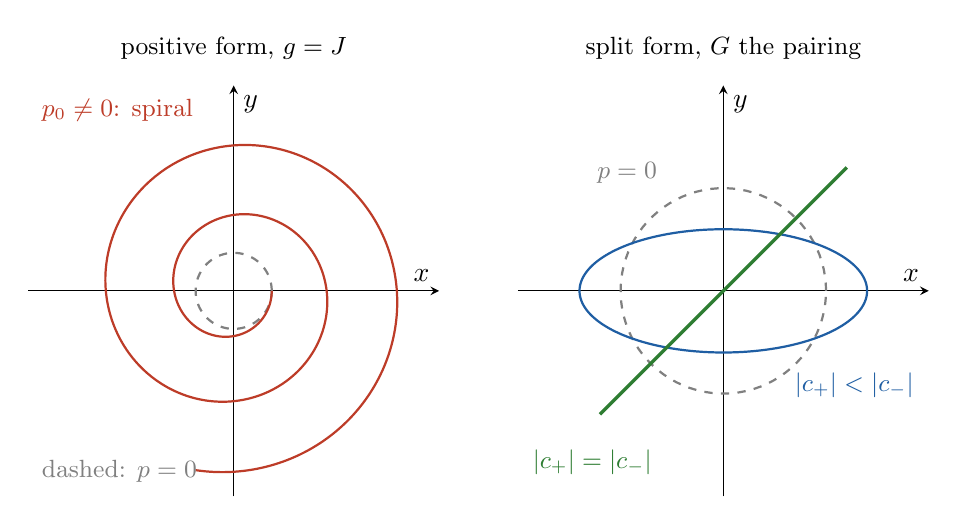
\begin{tikzpicture}
\begin{axis}[name=left,width=6.8cm,height=6.8cm,axis equal image,xmin=-5.4,xmax=5.4,ymin=-5.4,ymax=5.4,
  axis lines=middle,xtick=\empty,ytick=\empty,xlabel={$x$},ylabel={$y$},
  title={\small positive form, $g=J$}]
\addplot[gray,dashed,thick,domain=0:360,samples=90] ({cos(x)},{sin(x)});
\addplot[scol,thick,domain=0:5*pi,samples=600,variable=\t] ({cos(deg(\t))+0.3*\t*sin(deg(\t))},{-sin(deg(\t))+0.3*\t*cos(deg(\t))});
\node[scol,anchor=north west,font=\small] at (axis cs:-5.3,5.3) {$p_0\neq0$: spiral};
\node[gray,anchor=south west,font=\small] at (axis cs:-5.3,-5.3) {dashed: $p=0$};
\end{axis}
\begin{axis}[at={(left.east)},anchor=west,xshift=1.0cm,width=6.8cm,height=6.8cm,axis equal image,xmin=-2.0,xmax=2.0,ymin=-2.0,ymax=2.0,
  axis lines=middle,xtick=\empty,ytick=\empty,xlabel={$x$},ylabel={$y$},
  title={\small split form, $G$ the pairing}]
\addplot[gray,dashed,thick,domain=0:360,samples=90] ({cos(x)},{sin(x)});
\addplot[tcol,thick,domain=0:360,samples=180] ({1.4*cos(x)},{-0.6*sin(x)});
\addplot[gcol,very thick,domain=0:360,samples=180] ({0.85*cos(x)-0.85*sin(x)},{0.85*cos(x)-0.85*sin(x)});
\node[tcol,anchor=north east,font=\small] at (axis cs:1.95,-0.7) {$|c_+|<|c_-|$};
\node[gcol,anchor=north west,font=\small] at (axis cs:-1.95,-1.45) {$|c_+|=|c_-|$};
\node[gray,anchor=south east,font=\small] at (axis cs:-0.55,0.95) {$p=0$};
\end{axis}
\end{tikzpicture}
\caption{Interior motion in one pairing plane (\cref{ex:oneplane}). Left: with the positive form and an antisymmetric shift the
zero-momentum orbits are circles, and any momentum turns them into outward spirals, as \cref{thm:virial} requires. Right: with the split form
and the binding root $G$ every orbit is closed; the zero-momentum orbits are circles, the momentum-carrying ones ellipses, degenerating to a
segment when the two rotating parts have equal size.}
\label{fig:interior}
\end{figure}

\subsection{The orbits as duality rotations}

Read through the field-strength dictionary of \cref{thm:emfield}, an interior configuration $X$ is a two-form and the binding root is the
Hodge star. The bound motion then has a transparent meaning.

\begin{proposition}[Bound orbits in field-strength language]
\label{prop:orbitsEM}
Let $G$ be the pairing \eqref{eq:Gpair} and $z=\bB+i\bE$.
\begin{enumerate}[label=(\roman*),leftmargin=2.2em]
\item The zero-momentum orbits are $X(\tau)=e^{-\kappa G\tau}X_0$, that is $z(\tau)=e^{-i\kappa\tau}z_0$: continuous duality rotations, along which
$q(z(\tau))=e^{-2i\kappa\tau}q(z_0)$. A non-null orbit is a single spacetime plane at exactly four instants per period, alternately of magnetic
and electric type, and a null orbit is a single plane at every instant.
\item Every solution is $z(\tau)=c_-e^{-i\kappa\tau}+c_+e^{i\kappa\tau}$ with $c_\pm\in\C^3$, the momentum corresponds to $2i\kappa c_+e^{i\kappa\tau}$, and the
period averages are
\[
\langle q\rangle=2\,c_-\cdot c_+,\qquad \langle\bE\cdot\bB\rangle=\Im(c_-\cdot c_+),\qquad \langle|\bB|^2-|\bE|^2\rangle=2\Re(c_-\cdot c_+).
\]
\item The energy is $\mathcal E=2m\kappa^2\Re(c_-\cdot c_+)$, and the complex quantity $\tfrac m2\bigl(q(\dot z)+\kappa^2q(z)\bigr)=2m\kappa^2\,c_-\cdot c_+$ is
conserved; its imaginary part is a second constant of motion.
\item On the orbits with $c_+=\bar c_-$ the vector $z$ is real at every instant: $\bE=0$ and $\bE\cdot\bB=0$ throughout, while the momentum is not
zero.
\end{enumerate}
\end{proposition}

On a zero-momentum orbit $\bE\cdot\bB(\tau)=\tfrac12|q_0|\sin(\phi_0-2\kappa\tau)$ with $q_0=|q_0|e^{i\phi_0}$, and the rest-frame field of
\cref{sec:orth} turns from purely magnetic through screws to purely electric and back, at the fixed rest-frame energy density
$\tfrac12|q_0|$. So the binding flow is what breaks orthogonality on every non-null orbit without momentum, while orbits that carry momentum
can stay orthogonal throughout. The mean non-orthogonality and the energy of a general orbit are the imaginary and real parts of one conserved
complex number $c_-\cdot c_+$, and neither determines the other.

\begin{theorem}[The parity-odd term is a total derivative]
\label{thm:EBsplit}
For the split-form Lagrangian with the pairing,
\[
\mathcal L_\kappa=\frac m2\Bigl(\eta(\dot X,\dot X)-\kappa^2\eta(X,X)\Bigr)-m\kappa\,\frac{d}{d\tau}\bigl(\bE\cdot\bB\bigr).
\]
Consequently the cross term has identically vanishing Euler--Lagrange expression, the equation $\ddot X=-\kappa^2X$ comes from the first bracket
alone, and the momenta of $\mathcal L_\kappa$ and $\mathcal L_{-\kappa}$ differ by $2m\kappa\,\eta GX$. Parity maps $\mathcal L_\kappa$ to $\mathcal L_{-\kappa}$
and exchanges the orbits without momentum with those carried entirely by the counter-rotating part, while $C$ and $T$ leave $\mathcal L_\kappa$
invariant.
\end{theorem}

\begin{proof}
$G$ is $\eta$-self-adjoint, so $\tfrac{d}{d\tau}\eta(X,GX)=2\eta(\dot X,GX)$, and $\eta(X,GX)=-2\,\bE\cdot\bB$ by \cref{thm:emfield}; $\eta(GX,GX)=-\eta(X,X)$
because $G$ is an anti-isometry. Expanding $\eta(\dot X+\kappa GX,\dot X+\kappa GX)$ gives the formula. Parity reverses $\bE$ and fixes $\bB$, so
$PGP^{-1}=-G$ and $P$ acts on $z$ as complex conjugation.
\end{proof}

The binding term carries the one parity-odd ingredient of the interior, the sign of $\kappa$, and it sits entirely in a total derivative.
Since $\bE\cdot\bB$ is a single-valued function on the configuration space, the canonical transformation $p\mapsto p+2m\kappa\,\eta GX$ removes it,
classically and as a phase of wave functions. The structure is that of the $\theta$-term of electrodynamics, a parity-odd coefficient times a
total derivative, with the difference that here it has no topological sector in which to act. In the positive form the same cross term is
gyroscopic, with Euler--Lagrange expression $2m\kappa G\dot X$, and the sign of $\kappa$ enters the equations of motion; that is another way of
seeing why the two forms behave so differently.

\subsection{What the binding root selects, and what tears it}

The binding root is not merely available; it carries structure. By \cref{thm:GLorentz} its centraliser is a Lorentz algebra $\lG$, not
conjugate to the interior one (\cref{prop:notconj}). The same operator limits what transport can do to the bound sector.

\begin{proposition}[Transport and a homogeneous threshold]
\label{prop:tear}
Let a connection along the path take values $\omega$ in $\so{3,3}$. If $\omega$ lies in the compact part of $\lG$, transport and the shift commute
and the orbit is carried rigidly. If $\omega$ has a boost component of strength $c$ in a pairing plane $(e_a,e_{a+3})$, the homogeneous $2\times2$
block there has exponents $\pm\sqrt{c^2-\kappa^2}$: oscillatory for $c<\kappa$ and real for $c>\kappa$.
\end{proposition}

\begin{proof}
In the basis $(e_a,e_{a+3})$ the boost generator is $\sigma=\bigl(\begin{smallmatrix}0&1\\1&0\end{smallmatrix}\bigr)$ and $G$ is
$\bigl(\begin{smallmatrix}0&-1\\1&0\end{smallmatrix}\bigr)$, so $-c\sigma+\kappa G=\bigl(\begin{smallmatrix}0&-c-\kappa\\-c+\kappa&0\end{smallmatrix}\bigr)$, whose
square is $(c^2-\kappa^2)\id$.
\end{proof}

The threshold classifies exponents of the homogeneous block, not boundedness of the full flow, and the difference is real. With the momentum
included, the phase-space generator $M=\bigl(\begin{smallmatrix}-c\sigma-\kappa G&\id/m\\0&-c\sigma+\kappa G\end{smallmatrix}\bigr)$ satisfies
$M^2-(c^2-\kappa^2)\id=\bigl(\begin{smallmatrix}0&-2c\sigma/m\\0&0\end{smallmatrix}\bigr)$, nilpotent and nonzero for $c\neq0$. At $\kappa=m=1$ and
$c=\tfrac12$ one finds $\det(\lambda\id-M)=(\lambda^2+\tfrac34)^2$ with $\rank(M^2+\tfrac34\id)=2$: Jordan blocks, and generic secular growth strictly
below the threshold. Along an open path, moreover, a connection coefficient can be changed by a frame rotation, so growth on one worldline
proves nothing; the invariant is the holonomy around a closed path. \Cref{sec:curved} computes it in an explicit curved model and finds that
normal curvature converts zero-momentum orbits into momentum-carrying ones, through exactly the failure of the normal rotation to commute with
$G$.

What this part delivers is a bound sector, a frequency, a centralising Lorentz algebra and an exponent threshold, all from an adopted binding
operator. It does not deliver a spectrum: $\kappa$ is not fixed, the single frequency is degenerate across the three pairs, and the energy is
indefinite, so these are bound orbits and not bound states in any quantum sense. Nor does it settle the relation between the two square roots of
the pairing beyond \cref{lem:Gclifford}: $\cK$ is $\eta$-antisymmetric and grades, $G$ is $\eta$-self-adjoint and binds, and they differ by the
Cartan involution $\Ad_{e_1e_2e_3}$.

\section{Closing the force law}
\label{sec:closure}

The force law $\dot p=\kappa G^{\!\top}p$ carries its rate $\kappa$ as a constant put in by hand. A force law of this shape is familiar from
rigid bodies and ideal fluids, where the equation of motion is a geodesic equation on a Lie group and the rate is itself dynamical. This
section asks whether the interior law can be closed in that sense: whether there is a Lie--Poisson system whose bracket and inertia are built
from the same data that build $G$, and whose solutions contain the force law with $\kappa$ as a dynamical variable. A bracket or an inertia is
called \emph{derived from the Clifford structure} when it is equivariant under the algebra $\lG$ of \cref{thm:GLorentz} and built from
$\eta$, $G$ and the bivectors. The answers, in brief: no closure lives on the frame alone; the closure on one extra direction is unique; its
inertia is constrained by two requirements that exclude each other; and the dynamics it generates is a pendulum in the duality angle that
drifts the frame except on null data.

Throughout, $V=\R^{3,3}$, a covector $p$ is a column with $\langle p,X\rangle=p^{\!\top}X$, $\pi=\eta^{-1}p$, and $z(X)=x+iy$ for
$X=\sum_j(x_je_j+y_je_{j+3})$, so that $G$ acts as $i$. For a covector put
\begin{equation}
\label{eq:wdef}
C(p)=p^{\!\top}\eta^{-1}p,\qquad D(p)=p^{\!\top}G\eta^{-1}p,\qquad w(p):=q\bigl(z(\pi)\bigr)=C(p)-iD(p).
\end{equation}
In the field-strength reading, with $(\bB;\bE)=\pi$, $w=|\bB|^2-|\bE|^2+2i\,\bB\cdot\bE$ is the complex invariant of the field carried by the
momentum.

\subsection{The force law as a dual transport}

Euler--Arnold equations are geodesic equations on a Lie group with a one-sided invariant metric \cite{Arnold66,ArnoldKhesin98}; for a
left-invariant metric they read $\dot\mu=\ad_w^{\!\top}\mu$ with $\mu=Aw$ for an inertia $A$. The rigid body is the case of $SO(3)$, where this is
$\dot{\mathbf M}=\mathbf M\times\boldsymbol\Omega$, and incompressible Euler flow the case of the volume-preserving diffeomorphisms.

\begin{proposition}[The dictionary]
\label{prop:EAdict}
\begin{enumerate}[label=(\roman*),leftmargin=2.2em]
\item Since $\langle G^{\!\top}p,v\rangle=\langle p,Gv\rangle$, the law $\dot p=\kappa G^{\!\top}p$ transports the covector $p$ by the transpose of $\kappa G$.
It is the Lie--Poisson equation $\dot p=\ad_w^{\!\top}p$ of a Lie bracket on the frame exactly when $\kappa G=\ad_w$ is an inner derivation.
\item For a bracket with trivial centre on the $6n$-dimensional frame the inner derivations fill a $6n$-dimensional subspace of $\so{3n,3n}$, of
dimension $3n(6n-1)$, when $\eta$ is invariant: a fraction $2/(6n-1)$.
\item When $\kappa G=\ad_u$ and $p=Au$, the shift operators $\alpha_\pm=\partial_\tau\pm\kappa G$ are the constrained variations
$\delta u=\dot\xi\pm[u,\xi]$ of Euler--Poincar\'e reduction \cite{MarsdenRatiu99,HolmMarsdenRatiu98}, in the body and in the spatial frame.
\end{enumerate}
\end{proposition}

\begin{proposition}[The binding root is inner for no bracket]
\label{prop:EAnotinner}
For every Lie bracket and every $w$, $\ad_w(w)=0$, so every inner derivation is singular. The binding root satisfies $G^2=-\id$ and is
invertible, so $\kappa G$ is inner for no Lie bracket on $\R^{3n,3n}$, invariant or not, and the force law with that $G$ is never a
Lie--Poisson equation on the frame itself. It is one on the extension $\R\hat g\ltimes\R^{3n,3n}$, the frame taken abelian and $\hat g$ acting on
it by $G$, where it is the Lie--Poisson equation of the fixed element $\kappa\hat g$ restricted to the ideal.
\end{proposition}

\begin{theorem}[Transport and factorisation are complementary]
\label{thm:EAdichotomy}
$\End(\R^{3n,3n})=\so{3n,3n}\oplus\{G:G=G^\dagger\}$, of dimensions $3n(6n-1)+3n(6n+1)=36n^2$. Along $\dot p=\kappa G^{\!\top}p$ the Casimir
$C=\eta^{-1}(p,p)$ changes at the rate $dC/d\tau=2\kappa\,p^{\!\top}G\eta^{-1}p$, which vanishes for every $p$ exactly when $G$ lies in the first
summand, while factorisation in the split form requires the second. The binding root lies in the second summand and moves the Casimir at the rate
$dC/d\tau=-4\kappa\,\bB\cdot\bE$ in the variables $(\bB;\bE)=\eta p$.
\end{theorem}

At the first rung the frame itself is a Lie algebra. With $L_i=e_i$ and $K_i=e_{i+3}$ obeying the brackets of \cref{thm:emfield}, $\R^{3,3}$
becomes $\so{1,3}$ with Killing form $-4\eta$; in the variable $z=\bB+i\bE$ the bracket is the complex cross product, $G$ is multiplication by $i$
and lies in the centroid, $[Gx,y]=G[x,y]$, and $z\cdot z$ is the form $q$. The inner derivations fill six of the fifteen dimensions of
$\so{3,3}$. Closing the force law into an Euler--Arnold equation on the frame would need a bracket for which the shift is inner, and by
\cref{prop:EAnotinner} there is none. A closure must leave the frame.

\subsection{No closure on the frame; the rotor is unique}

\begin{proposition}[Equivariant maps and forms]
\label{prop:lGhoms}
For $\lG=\operatorname{span}\{L_i,K_i\}$: $\Hom_{\lG}(V,V)=\operatorname{span}\{\id,G\}$ and $\Hom_{\lG}(V,\R)=0$;
$\Hom_{\lG}(\Lambda^2V,V)=\operatorname{span}\{\beta_0,G\beta_0\}$, where $\beta_0(X,Y)$ is the complex cross product $z(X)\times z(Y)$ returned to
$V$, and $\Hom_{\lG}(\Lambda^2V,\R)=0$; and the $\lG$-invariant symmetric forms on $V^*$ are $\operatorname{span}\{\eta^{-1},G\eta^{-1}\}$.
\end{proposition}

\begin{theorem}[The brackets on the frame]
\label{thm:brackets}
The $\lG$-equivariant Lie brackets on $V$ are $\beta_L=L\beta_0$ with $L=a+bG$. The bracket $\beta_0$ makes $(V,\beta_0)\cong\lG$, its derivations
are the six inner ones, its centroid is $\operatorname{span}\{\id,G\}\cong\C$, so $G$ is not a derivation, and $\beta_L$ has Killing form
$-4\bigl[(a^2-b^2)\eta+2ab\,\eta G\bigr]$.
\end{theorem}

\begin{proof}
By \cref{prop:lGhoms} every equivariant antisymmetric bilinear map is $(c_1+c_2G)\beta_0$. Since $L$ lies in the centroid,
$\beta_L(\beta_L(X,Y),Z)=L^2\beta_0(\beta_0(X,Y),Z)$, and $\beta_L$ inherits the Jacobi identity.
\end{proof}

\begin{theorem}[No closure on the frame alone]
\label{thm:noframe}
Let $L=a+bG\neq0$. For every symmetric $N$, with $\mathfrak g^*$ identified with $\mathfrak g$ through $\eta$, the Euler--Arnold field
$\beta_0(M,NM)$ conserves $\eta(M,M)$ and $\eta(M,GM)$, whereas along the force law, in the form $\dot M=\kappa GM$,
$\tfrac{d}{d\tau}\eta(M,M)=2\kappa\,\eta(M,GM)$ and $\tfrac{d}{d\tau}\eta(M,GM)=-2\kappa\,\eta(M,M)$. No Hamiltonian flow on $(V,\beta_L)^*$ coincides
with the force law on an open set, and this remains true with a state-dependent rate.
\end{theorem}

\begin{proof}
The two quadratic forms are the Casimirs of $(V,\beta_L)^*$ and are conserved by every Hamiltonian flow, while the force law rotates them into
each other. Equality on an open set would make both vanish there, that is $z\cdot z=0$ on an open set, which no nonzero polynomial does. For a
state-dependent rate, the equations $\beta_0(M_s,NM_s)=f_s\,GM_s$ at twelve rational null vectors already force every $f_s=0$ and
$N\in\operatorname{span}\{\id,G\}$, for which $\beta_0(M,NM)\equiv0$.
\end{proof}

A closure therefore needs a direction beyond the frame. Adjoin one generator $\hat g$, the \emph{rotor}, on which $\lG$ acts trivially; the rate
$\kappa$ is a Lorentz scalar, since $G$ commutes with $\lG$.

\begin{theorem}[Uniqueness of the closure]
\label{thm:closureunique}
Let $\mathfrak s=\R\hat g\oplus V$ carry an $\lG$-equivariant Lie bracket for which $\ad_{\hat g}$ does not vanish on $V$. Then
$[\hat g,X]=(a+bG)X$ and $[X,Y]=0$ for $X,Y\in V$, with $(a,b)\neq(0,0)$. If moreover the rotor rotates the frame covector without dilating it,
as the force law does, then $a=0$ and, after rescaling $\hat g$, $\mathfrak s\cong\R\ltimes_GV$: $[\hat g,X]=GX$, $[X,Y]=0$.
\end{theorem}

\begin{proof}
Equivariance gives $[\hat g,X]=AX+\alpha(X)\hat g$ with $A\in\operatorname{span}\{\id,G\}$ and $\alpha=0$, and $[X,Y]=(c_1+c_2G)\beta_0(X,Y)$, the
$\hat g$-component vanishing by \cref{prop:lGhoms}. The Jacobi identity for $(\hat g,X,Y)$ reads $(a+bG)(c_1+c_2G)\beta_0(X,Y)=0$, a linear system in
$(c_1,c_2)$ with determinant $a^2+b^2\neq0$, so $c_1=c_2=0$. On $\mathfrak s^*$ the rotor acts on $p$ through $(a+bG)^{\!\top}$, and
$\tfrac{d}{d\tau}|p|^2=2a\,(h/I_0)|p|^2$ because $G$ is antisymmetric; a pure rotation needs $a=0$.
\end{proof}

The extension of \cref{prop:EAnotinner} is therefore not one choice among several: it is the only equivariant closure. The frame is abelian,
all the dynamics sits in the rotor, and the rotor acts by the binding root itself. With several constituents the argument runs factor by
factor, since equivariant maps between distinct constituents vanish, and a common rotation rate gives $\mathfrak s_n=\R\ltimes_{G_n}V_n$ with
$G_n=\bigoplus_kG$.

\subsection{The Lie--Poisson dynamics, and the two interiors as clamped reductions}

\begin{proposition}[Lie--Poisson equations]
\label{prop:LP}
On $\mathfrak s^*$ with coordinates $(h,p)$ let $H=h^2/(2I_0)+\tfrac12p^{\!\top}Np$, with $I_0>0$ the rotor inertia and $N$ a symmetric form on
$V^*$, the inverse frame inertia. The Lie--Poisson equations are
\begin{equation}
\label{eq:LProtor}
\dot p=\frac h{I_0}\,G^{\!\top}p,\qquad \dot h=-\,p^{\!\top}GNp ,
\end{equation}
so the force law holds with the dynamical rate $\kappa=h/I_0$, and $|p|^2$ is a Casimir. For $p\neq0$ the coadjoint orbit through $(h,p_0)$ is the
cylinder $\R\times\{e^{\theta G}p_0\}\cong T^*S^1$, on which $(\theta,h)$ are canonical for $h^2/(2I_0)+U(\theta)$ with
$U(\theta)=\tfrac12p(\theta)^{\!\top}Np(\theta)$ and $p(\theta)=e^{-\theta G}p_0$: every reduced motion is a motion of the rotor angle alone.
\end{proposition}

\begin{proposition}[The two interiors are clamped reductions]
\label{prop:groupred}
On the group $S$ with product $(\theta,x)(\theta',x')=(\theta+\theta',x+e^{\theta G}x')$ let $L=\tfrac12I_0\dot\theta^2+\tfrac m2\eta(u,u)$ with body velocity
$u=e^{-\theta G}\dot x$, and put $X=e^{-\theta G}x$. Then $u=\dot X+\dot\theta\,GX$, the Euler--Lagrange equations are \eqref{eq:LProtor} with $N=\eta^{-1}/m$,
and clamping $\theta=\kappa\tau$ gives
\[
L=\tfrac12I_0\kappa^2+\tfrac m2\,\eta\bigl(\dot X+\kappa GX,\ \dot X+\kappa GX\bigr),
\]
the split-form interior \eqref{eq:splitL}. With $\tfrac m2|u|^2$ in place of $\tfrac m2\eta(u,u)$ the clamped Lagrangian is the positive-form interior
\eqref{eq:alpha} with $g=G$.
\end{proposition}

So the two interiors of \cref{sec:shifted,sec:neutral} are the clamped reductions of one closure, with inverse inertias $N=\eta^{-1}/m$ and
$N=\id/m$. Which inertias the Clifford data permit is the next question.

\subsection{Two requirements on the inertia}

\begin{definition}[The two requirements]
\label{def:inertiareq}
A symmetric $N$ on $V^*$ satisfies the \emph{Lorentz requirement} if it is $\lG$-invariant, $rN+Nr^{\!\top}=0$ for all $r\in\lG$, and the
\emph{duality requirement} if the rate $h/I_0$ is conserved for all data. Write $N=N_c+N_a$ with $N_c=\tfrac12(N-GNG)$ commuting and
$N_a=\tfrac12(N+GNG)$ anticommuting with $G$.
\end{definition}

\begin{theorem}[The two requirements exclude each other]
\label{thm:inertiareq}
\begin{enumerate}[label=(\roman*),leftmargin=2.2em]
\item $N_c$ and $N_a$ are symmetric; the commuting forms have dimension $9$ and the anticommuting ones $12$.
\item The Lorentz requirement gives $N=(a\eta^{-1}+bG\eta^{-1})/m$, a two-dimensional family inside the anticommuting forms, with frame energy
$\tfrac12p^{\!\top}Np=\Re\bigl((a+ib)w(p)\bigr)/(2m)$.
\item The duality requirement holds exactly when $[N,G]=0$. Among the forms invariant under the compact part of $\lG$ the only ones commuting with
$G$ are the multiples of $\id$: the positive form.
\item The two requirements meet in $0$, and they do not exhaust the symmetric forms: $N=(2\,\id+\eta^{-1})/m$ is positive definite and satisfies
neither.
\end{enumerate}
\end{theorem}

In the field-strength reading the dichotomy is the classical one. The Lorentz class consists of the two invariants $|\bB|^2-|\bE|^2$ and
$\bB\cdot\bE$; the duality class contains the energy density $|\bB|^2+|\bE|^2$; and a duality rotation preserves the energy density while it
rotates the Lagrangian density \cite{Calkin65,DeserTeitelboim76,GaillardZumino81}. The split form lies in the Lorentz class and the positive form
in the duality class.

\begin{theorem}[The frame under the closure]
\label{thm:drift}
Reconstruct the group curve from the body velocity,
\[
(\theta,x)^{-1}\tfrac{d}{d\tau}(\theta,x)=(h/I_0,\,Np),\qquad \theta(0)=0 .
\]
Then $p=e^{-\theta G}p_0$ and
\[
\dot x=\bigl(N_c+e^{2\theta G}N_a\bigr)p_0,\qquad \dot h=-\,p_0^{\!\top}Ge^{2\theta G}N_ap_0 .
\]
With the rotor clamped at $\theta=\kappa\tau$, $\kappa\neq0$,
\[
x(\tau)=x_0+\tau\,N_cp_0+\bigl(e^{2\kappa\tau G}-\id\bigr)(2\kappa G)^{-1}N_ap_0 ,
\]
so the frame stays bounded for all data exactly when $N_c=0$ and drifts at the velocity $N_cp_0$ otherwise, while the rate is constant for all data
exactly when $N_a=0$.
\end{theorem}

A clamped rate that is also the dynamical one, and a bounded clamped frame, are therefore exclusive requirements: each is met by one summand of
$\mathrm{Sym}(V^*)=\mathrm{Sym}_c\oplus\mathrm{Sym}_a$. For $N=\id/m$ the rate is conserved and the frame drifts at $p_0/m$, which is the
non-recurrence of \cref{thm:virial}, $X=e^{-\kappa\tau G}(X_0+\tau p_0/m)$; for $N=\eta^{-1}/m$ the clamped frame is bounded, as in \cref{thm:neutral},
but the rate is conserved only on null data.

\subsection{The free rotor: a pendulum in the duality angle}

\begin{theorem}[The duality pendulum]
\label{thm:pendulum}
Let $N=(a\eta^{-1}+bG\eta^{-1})/m$ and write $(a+ib)w(p_0)=R_0e^{i\varphi_0}$, $R_0\ge0$. Along the flow $z(\pi)$ turns as $e^{i\theta}$ and
$w(p)=e^{2i\theta}w(p_0)$, the frame energy is $U(\theta)=\tfrac{R_0}{2m}\cos(2\theta+\varphi_0)$, and
\[
I_0\ddot\theta=\frac{R_0}m\sin(2\theta+\varphi_0),\qquad E_\theta=\tfrac12I_0\dot\theta^2+\frac{R_0}{2m}\cos(2\theta+\varphi_0)=H .
\]
With $\psi:=2\theta+\varphi_0$ this is the pendulum $\ddot\psi=(2R_0/mI_0)\sin\psi$, stable at $\psi=\pi$. The rotor angle is the duality angle of
the momentum field, and the potential is its Lorentz-invariant frame energy.
\end{theorem}

\begin{figure}[t]
\centering
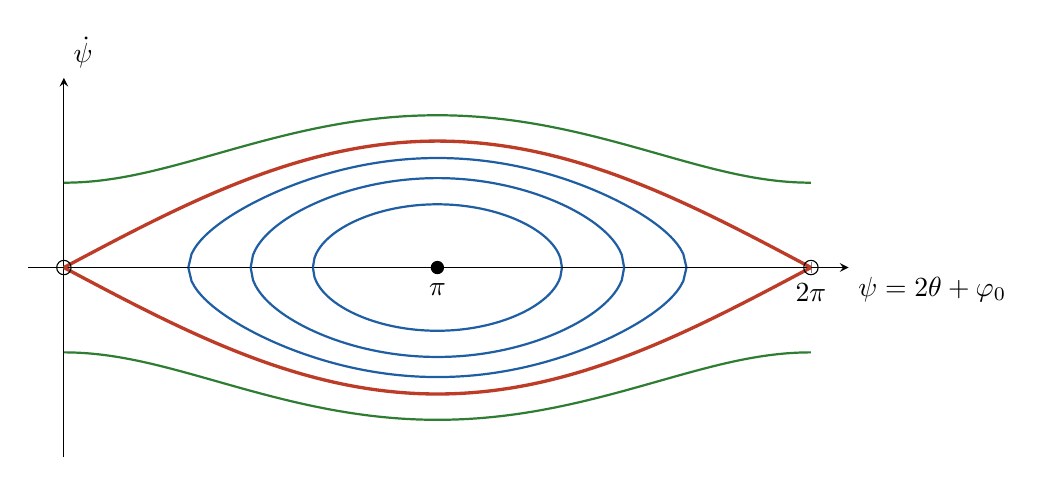
\begin{tikzpicture}
\begin{axis}[width=12cm,height=6.4cm,xmin=-0.3,xmax=6.6,ymin=-3.0,ymax=3.0,
  axis lines=middle,xlabel={$\psi=2\theta+\varphi_0$},ylabel={$\dot\psi$},
  xtick={0,3.14159,6.28318},xticklabels={$0$,$\pi$,$2\pi$},ytick=\empty,
  xlabel style={anchor=north west},ylabel style={anchor=south west}]
\foreach \E/\a in {-0.5/2.0944,0/1.5708,0.5/1.0472}{
  \addplot[tcol,thick,domain=\a:{2*pi-\a},samples=160] {sqrt(max(0,2*(\E-cos(deg(x)))))};
  \addplot[tcol,thick,domain=\a:{2*pi-\a},samples=160] {-sqrt(max(0,2*(\E-cos(deg(x)))))};
}
\addplot[scol,very thick,domain=0:2*pi,samples=200] {2*abs(sin(deg(x/2)))};
\addplot[scol,very thick,domain=0:2*pi,samples=200] {-2*abs(sin(deg(x/2)))};
\addplot[gcol,thick,domain=0:2*pi,samples=160] {sqrt(2*(1.9-cos(deg(x))))};
\addplot[gcol,thick,domain=0:2*pi,samples=160] {-sqrt(2*(1.9-cos(deg(x))))};
\addplot[only marks,mark=*,mark size=2.2pt,black] coordinates {(3.14159,0)};
\addplot[only marks,mark=o,mark size=2.6pt,black] coordinates {(0,0) (6.28318,0)};
\end{axis}
\end{tikzpicture}
\caption{Phase portrait of the duality pendulum (\cref{thm:pendulum}), in units with $2R_0/(mI_0)=1$; the filled dot is the stable point
$\psi=\pi$ and the open dots the unstable one. Blue: librations, in which the rate $\kappa=\dot\theta$ changes sign periodically and the duality
rotation reverses. Red: the separatrix. Green: rotations, in which the rotor turns for all time with a modulated rate. The constant-rate law of \cref{sec:neutral} is the limit of large rotor energy, far above the
separatrix (\cref{cor:multiscale}).}
\label{fig:pendulum}
\end{figure}

\begin{corollary}[When the rate is constant]
\label{cor:constrate}
With Lorentz-class inertia the rate is constant and nonzero along the flow exactly when $R_0=0$ and $h(0)\neq0$; $R_0=0$ means $(a,b)=(0,0)$ or
$w(p_0)=0$, that is $|\bB|=|\bE|$ and $\bB\cdot\bE=0$ for the field of $\pi_0$: a null field, the class that contains plane waves
\cite{Synge56,Robinson61}.
\end{corollary}

\begin{corollary}[The multiscale criterion]
\label{cor:multiscale}
Let $R_0>0$, $\kappa_0:=\dot\theta(0)\neq0$, $\psi_0=2\theta(0)+\varphi_0$ and $\varepsilon:=R_0/(mI_0\kappa_0^2)$. Then
$\kappa^2=\kappa_0^2\bigl[1+\varepsilon(\cos\psi_0-\cos\psi)\bigr]$. The rotor turns for all time exactly when $\varepsilon(1-\cos\psi_0)<1$, and $\varepsilon<\tfrac12$
suffices for every phase, in which case $|\kappa^2/\kappa_0^2-1|\le2\varepsilon$. At $\varepsilon(1-\cos\psi_0)=1$ the motion is the separatrix, and beyond it
the rotor librates and the duality rotation reverses. The constant-rate law is the limit $\varepsilon\to0$, and the multiscale requirement is
\begin{equation}
\label{eq:multiscale}
I_0\,\kappa_0^2\ \gg\ R_0/m .
\end{equation}
\end{corollary}

A clamped rotor is therefore an idealisation of a heavy one. It is not a harmless idealisation, because the frame feels the modulation.

\begin{theorem}[The free rotor drifts the frame]
\label{thm:freedrift}
Let $N$ be of Lorentz class with $R_0>0$ and $\kappa_0\neq0$, in the rotating regime. During one period of the rate, while $\theta$ changes by $\pi$,
the frame is displaced by
\[
\Delta x=\lambda\,e^{-\varphi_0G}Np_0,\qquad \lambda=\tfrac12\int_0^{2\pi}\frac{\cos\psi\,d\psi}{|\kappa_0|\sqrt{1+\varepsilon(\cos\psi_0-\cos\psi)}}>0,
\]
and its mean velocity is $\tfrac\varepsilon4e^{-\varphi_0G}Np_0+O(\varepsilon^2)$. Every rotating solution with $R_0\neq0$ therefore has an unbounded frame.
\end{theorem}

\begin{proof}
For Lorentz-class $N$, $N=N_a$ and $\dot x=e^{2\theta G}Np_0$. In the rotating regime $\dot\theta$ never vanishes, so $d\tau=|d\theta|/|\dot\theta|$, and
with $e^{2\theta G}=e^{-\varphi_0G}e^{\psi G}$ and $e^{\psi G}=\cos\psi+G\sin\psi$ the $\sin\psi$ part integrates to zero because $1/|\dot\theta|$ depends on
$\cos\psi$ only. Since $1/|\dot\theta|$ is a strictly increasing function of $\cos\psi$ when $R_0>0$, the integrand of $\lambda$ exceeds its value at
$\cos\psi=0$ wherever $\cos\psi>0$ and falls short of it where $\cos\psi<0$, so $\lambda>0$. Expanding to first order gives
$\lambda=\pi\varepsilon/(4|\kappa_0|)+O(\varepsilon^2)$ over a period $\pi/|\kappa_0|+O(\varepsilon)$.
\end{proof}

\begin{example}[A drift in closed form]
\label{ex:drift}
Take $p_0=e^1$ and $m=I_0=\kappa_0=1$, so that $w=1$, $\varphi_0=0$, $\varepsilon=1$ and $\dot\theta^2=1+2\sin^2\theta$. Writing
$(1-2s)/\sqrt{1+2s}=2/\sqrt{1+2s}-\sqrt{1+2s}$ with $s=\sin^2\theta$, the displacement per turn of the rotor is
\[
\Delta x=\bigl(8K(-2)-4E(-2)\bigr)e_1\approx0.6336081022\,e_1 ,
\]
with $K(m)=\int_0^{\pi/2}(1-m\sin^2t)^{-1/2}dt$ and $E(m)=\int_0^{\pi/2}(1-m\sin^2t)^{1/2}dt$ the complete elliptic integrals in the parameter $m$
\cite{DLMF}. A numerical integration of the full system, frame included, reproduces this value to ten digits and returns $h$ and $p$ to their
initial values after each turn.
\end{example}

The clamped frame of \cref{thm:drift} moves on a circle of diameter $|Np_0|/|\kappa_0|$, while the free rotor adds $\tfrac{\pi\varepsilon}{2|\kappa_0|}|Np_0|$
per turn to first order, so the constant-rate picture tracks the bounded orbit for about $2/(\pi\varepsilon)$ turns. With Lorentz-class inertia and a
free rotor, a constant rate and a bounded frame coexist exactly on null data.

\begin{proposition}[Several constituents and one rotor]
\label{prop:several}
Let one rotor act on $n$ constituents with $N_k=(a_k\eta^{-1}+b_kG\eta^{-1})/m_k$ and $w_k=w(p^{(k)})$. Then $\dot w_k=2i(h/I_0)w_k$ for every $k$, all
forces carry the common phase $e^{2i\theta}$, and with $R_{\rm eff}e^{i\varphi_{\rm eff}}:=\sum_k(a_k+ib_k)w_k(0)/m_k$ the rotor obeys
$I_0\ddot\theta=R_{\rm eff}\sin(2\theta+\varphi_{\rm eff})$. The \emph{balance surface} $R_{\rm eff}=0$ is preserved by the flow; on it the rate is exactly
constant although no $w_k$ need vanish, and every frame moves on a bounded orbit. With equal inertias, $p^{(2)}=-Gp^{(1)}$ gives $w_2=-w_1$.
\end{proposition}

The Clifford data $\eta$, $G$, $G\eta^{-1}$ and $\beta_0$ are integer matrices. The rescaling $(I_0,m)\mapsto(sI_0,tm)$ preserves admissibility and
multiplies $\varepsilon$ by $1/(st)$, so no value of $\varepsilon$, and no ratio among $I_0$, $m$ and $|a+ib|$, is determined by the Clifford structure:
the form of the inertia is derived, and \eqref{eq:multiscale} is an input.

\subsection{Three constituents: the closure symmetry and the two projectors}

At $n=3$ write $e_A=e^{(k)}_i$ with $A=6(k-1)+i$; the temporal indices are $\{1,2,3,7,8,9,13,14,15\}$, each with its partner $i'=i+3$, and for
temporal $i<j$ put
\[
\mathrm{rot}(i,j):=e_{i'}e_{j'}-e_ie_j,\qquad \mathrm{bst}(i,j):=e_je_{i'}-e_ie_{j'} .
\]
For one constituent these span $\lG$, with $\mathrm{rot}(2,3)=2L_1$ and $\mathrm{bst}(2,3)=2K_1$ and cyclically up to sign. In this numbering the
weak directions of $P_*$ are $W=\{7,13,14,15\}$, the colour directions $\{10,11,12,16,17,18\}$, and $E$ denotes the span of the temporal directions
$\{7,8,9,13,14,15\}$ of constituents two and three; $G_3=G\oplus G\oplus G$.

\begin{theorem}[The closure symmetry is $\so{9,\C}$]
\label{thm:so9C}
$G_3$ is an anti-isometry of $\eta_3$ with $G_3^2=-\id$, and its centraliser in $\so{9,9}$ is $72$-dimensional, spanned by the $36$ paired rotations
and the $36$ paired boosts. In the basis of the nine temporal directions followed by their partners every element is
$\bigl(\begin{smallmatrix}R&S\\-S&R\end{smallmatrix}\bigr)$ with $R,S$ antisymmetric, and $R-iS$ identifies the centraliser with $\so{9,\C}$, whose
compact part consists of the paired rotations.
\end{theorem}

In the field-strength reading $V_3\cong\C^9$ carries three field strengths, and $\so{9,\C}$ consists of the complex orthogonal transformations of
$\sum_kz^{(k)}\cdot z^{(k)}$.

\begin{theorem}[No common Lorentz algebra]
\label{thm:nocommon}
The centraliser of $G_3$ meets the interior $\so{1,3}$ of the first constituent in $0$; the elements commuting with both $G_3$ and that algebra form
the $30$-dimensional $\so{6,\C}$ of paired elements of constituents two and three. Under $\lG^{(1)}$ the complexified spinor module is
$128\cdot(\tfrac12,\tfrac12)$, with no Weyl spinor.
\end{theorem}

No nonzero Lorentz generator leaves both the closure and the spinor structure of matter invariant: the two Lorentz algebras are different
subalgebras of $\so{9,9}$ with zero intersection, which is \cref{prop:notconj} lifted to three constituents. A Pati--Salam generator acts on the
closure variables only through its grade-two part, since $\ad_Z$ maps vectors to vectors exactly when $Z$ has grades zero and two. The intersection
with the Pati--Salam algebra can then be computed in general.

\begin{theorem}[The Pati--Salam algebra and the binding root]
\label{thm:PSbinding}
Let $U$ be any four-dimensional subspace of the span of the eight internal temporal directions, and $\mathfrak{ps}_U=\so U\oplus\so6_C$. Then neither
summand meets the centraliser of $G_3$, and
\[
\mathfrak{ps}_U\cap\Cent(G_3)=\bigl\{A+G_3AG_3^{-1}:\ A\in\so{U\cap E}\bigr\}\cong\so{U\cap E},
\]
of dimension $\binom d2\in\{1,3,6\}$ with $d=\dim(U\cap E)$. For the Pati--Salam algebra of $P_*$, $U=\operatorname{span}W\subset E$, and the
binding-compatible part is the diagonal $\so4_\Delta=\operatorname{span}\{\mathrm{rot}(i,j):i<j\in W\}\cong\su2\oplus\su2$, compact and non-abelian.
\end{theorem}

\begin{proof}
Let $A\in\so U$ and $B\in\so6_C$ with $[A+B,G_3]=0$, and split the internal temporal span as $E\oplus F$ with $F=\operatorname{span}\{e_2,e_3\}$. $G_3$ maps
$F$ into the interior plane $\operatorname{span}\{e_5,e_6\}$, where $A$ and $B$ vanish, so $Av=0$ for $v\in F$. For $v\in E$, $G_3v$ is a colour direction
and $Bv=0$, so $G_3Av=BG_3v$ lies in the colour span and $Av\in E$. Hence $A\in\so{U\cap E}$ and $B=G_3AG_3^{-1}$ on the colour span, and conversely.
Finally $d\ge4+6-8=2$.
\end{proof}

Neither Pati--Salam factor contains an element commuting with the binding root; the compatible part pairs every rotated temporal direction with
its spatial partner, which the colour $\su4$, acting on spatial directions alone, never does.

\begin{theorem}[What survives each projector]
\label{thm:survive}
\begin{enumerate}[label=(\roman*),leftmargin=2.2em]
\item The part of $\Cent(G_3)$ commuting with $\Pfam$ is $\operatorname{span}\{\mathrm{rot}(2,3),\mathrm{rot}(8,9),\mathrm{rot}(14,15),\mathrm{bst}(14,15)\}$,
abelian of dimension four. The kinetic condition holds for the two internal rotations and fails for $\mathrm{bst}(14,15)$, so the gauge-admissible
part is $\uu1^2=\operatorname{span}\{\mathrm{rot}(8,9),\mathrm{rot}(14,15)\}$.
\item The part commuting with $P_*$ is $\operatorname{span}\{\mathrm{rot}(2,3),\mathrm{rot}(8,9)\}\oplus\so4_\Delta$, compact of dimension eight, and its
internal part $\so4_\Delta\oplus\R\,\mathrm{rot}(8,9)$ acts faithfully and satisfies the kinetic condition.
\item Under either projector the frame Lorentz algebra $\lG^{(1)}$ keeps only $\mathrm{rot}(2,3)=e_5e_6-e_2e_3$, a rotation of the interior plane
$(e_5,e_6)$ locked to the rotation of the surplus pair.
\end{enumerate}
\end{theorem}

The rotor acts through $G_3$ and commutes with all of $\Cent(G_3)$, so a one-rotor closure is compatible with either projector. What differs is the
symmetry each leaves: an abelian one for $\Pfam$, and for $P_*$ the non-abelian diagonal of weak isospin and a colour $\so4$.

\begin{table}[t]
\centering
\small
\begin{tabular}{@{}lccccccccc@{}}
\toprule
$(q_1,q_2)$ & $(-1,-1)$ & $(-1,0)$ & $(-1,1)$ & $(0,-1)$ & $(0,0)$ & $(0,1)$ & $(1,-1)$ & $(1,0)$ & $(1,1)$\\
\midrule
left, $\Gamma=-1$ & 1 & 0 & 1 & 1 & 2 & 1 & 0 & 2 & 0\\
right, $\Gamma=+1$ & 0 & 2 & 0 & 1 & 2 & 1 & 1 & 0 & 1\\
\bottomrule
\end{tabular}
\caption{Weyl content of the block of $\Pfam$ under the two surviving charges $Q_1=-\tfrac12J\,\mathrm{rot}(8,9)$ and $Q_2=-\tfrac12J\,\mathrm{rot}(14,15)$:
the number of Weyl components with charges $(q_1,q_2)$ on each chirality half.}
\label{tab:closurecontent}
\end{table}

\begin{theorem}[Chirality and anomalies of what survives]
\label{thm:closurechiral}
With anomaly coefficients $\mathcal A(f)=\tfrac14\bigl[\Tr(fP_L)-\Tr(fP_R)\bigr]$ and charges $-JB$:
\begin{enumerate}[label=(\roman*),leftmargin=2.2em]
\item On $\Pfam$ the content is \cref{tab:closurecontent}; $\mathcal A\bigl((\alpha Q_1+\beta Q_2)^3\bigr)=-12\alpha\beta^2$ and $\mathcal A(\alpha Q_1+\beta Q_2)=0$, and
the left and right charge multisets coincide exactly when $\alpha\beta=0$. The anomaly-free subalgebras of $\uu1^2$ are $0$, $\R Q_1$ and $\R Q_2$,
each vector-like.
\item On $P_*$, with $\so4_\Delta=\su2_+\oplus\su2_-$ and $Q=-\tfrac12J\,\mathrm{rot}(8,9)$, the halves are
$L=(0,0)_0\oplus(\tfrac12,\tfrac12)_{+1}\oplus(1,0)_0$ and $R=(0,0)_0\oplus(\tfrac12,\tfrac12)_{-1}\oplus(0,1)_0$. For $H=\alpha H^+_3+\beta H^-_3+\gamma Q$,
$\mathcal A(H^3)=2\gamma(3\alpha^2+3\beta^2+4\gamma^2)$ and $\mathcal A(H)=8\gamma$, so the anomaly-free subalgebras are exactly those of $\so4_\Delta$, which
has neither a perturbative nor a global anomaly.
\item The two halves of $P_*$ carry inequivalent representations of $\so4_\Delta$, so it acts chirally; but every summand is a real representation
of $\su2\oplus\su2$, so the left-handed content is real and gauge-invariant Majorana masses exist \cite{Suzuki2000}. The chirality of $\so4_\Delta$
on $P_*$ forbids no mass.
\end{enumerate}
\end{theorem}

The rotor has no continuous lift to spinors: $(e^{\theta G})^{\!\top}\eta\,e^{\theta G}=\cos2\theta\,\eta+\sin2\theta\,\eta G$, so $e^{\theta G}$ is an isometry of
$\eta$ only for $\theta\in\pi\Z$, and at $\theta=\pi$, $e^{\pi G_3}=-\id$ is implemented by $\Gamma$. This excludes a coupling of the rotor through the
spin representation and says nothing about other couplings.

\begin{theorem}[Inertia freedom at three constituents]
\label{thm:inertia3}
The real dimensions of the symmetric forms on $V_3^*$ in the Lorentz class, $\{N,G_3\}=0$, and in the duality class, $[N,G_3]=0$, that are invariant
under a given symmetry are:
\begin{center}
\begin{tabular}{@{}lcc@{}}
\toprule
symmetry & Lorentz class & duality class\\
\midrule
$\Cent(G_3)=\so{9,\C}$ & $2$ & $0$\\
$\bigoplus_k\lG^{(k)}$ & $6$ & $0$\\
the $\Pfam$-surviving algebra & $18$ & $13$\\
the $P_*$-surviving algebra & $8$ & $6$\\
none & $90$ & $81$\\
\bottomrule
\end{tabular}
\end{center}
\end{theorem}

The Lorentz-class inertia is fixed up to one complex scale under the full closure symmetry and up to three under the single-constituent Lorentz
algebras, and imposing only what a projector leaves enlarges the freedom to nine complex scales for $\Pfam$ and four for $P_*$: neither projector
selects the inertia.

\subsection{Brackets supplied by hand}

The closure above is derived; one may also supply a bracket on the frame by hand and ask what the arena's own inertias do with it. A quadratic Lie
algebra whose invariant form is $\eta$ must have a maximal compact subalgebra of exactly half its dimension, and such \emph{balanced} simple real forms
are rare: a complex simple algebra regarded as real, $\su{p,q}$ with $|p-q|=1$, or $\so{p,q}$ with $(p,q)=\bigl(\tfrac{k(k+1)}2,\tfrac{k(k-1)}2\bigr)$, and
no exceptional form. At the first rung $\R^{3,3}$ admits exactly three semisimple quadratic structures, $\so{1,3}$, $\so4$ and $\so{2,2}$, and only
$\so{1,3}$ if $\eta$ is to be proportional to the Killing form. For $n\le20$ a simple closure exists exactly at $n=1,4,5,6,7,8,12,15,16,20$.

Two observations about the arena's inertias hold across these closures. With the split-form inertia $A=m\eta$, which is an invariant form, every
solution of the Euler--Arnold equation is a one-parameter subgroup and $\dot p\equiv0$. With the positive form $A=m\,\id$ on $\so{1,3}$ the system is
$\dot\bB=0$, $\dot\bE=\tfrac2m\bE\times\bB$: the magnetic half is frozen and the electric half precesses about it. The inertias with
$G^{\!\top}A^{-1}G=-A^{-1}$ form a twelve-dimensional family of holomorphic Euler tops $\dot Z=Z\times MZ$ with $M$ complex symmetric; they are Liouville
integrable and never positive definite.

At the rungs $n=(N^2-1)/3$ with $3\nmid N$, that is $(N,n)=(2,1),(4,5),(5,8),\dots$, the compact half of the balanced form $\slr{N,\C}_\R$ is $\su N$,
which is Zeitlin's finite truncation of two-dimensional incompressible Euler flow \cite{Zeitlin91}. Giving the 't~Hooft clock--shift modes the
discrete-Laplacian inertia, numerical integration at $N=4$ and $N=5$ conserves energy and enstrophy to $10^{-12}$ and moves up to $37\%$ of the
energy and $54\%$ of the enstrophy between Laplacian shells: transfer between scales inside the frame. With either of the arena's own inertias the same
data are exact equilibria, because both $\id$ and $\eta$ restrict to multiples of the invariant form on $\su N$. What the frame lacks for a fluid is
the inertia. Finally, no closure dissipates: every Euler--Arnold flow stays on a coadjoint orbit and preserves every Casimir, which is exactly what
viscosity destroys, so no closure of the force law can produce $\nu\Delta u$ on its own; and a constant generator that uniformly decreases the split
form $C$ has, by the inertia theorem of Ostrowski and Schneider \cite{OstrowskiSchneider62}, exactly $3n$ exponentially unstable directions.

\section{Rest energy in the closure}
\label{sec:restclosure}

The closure of \cref{sec:closure} is the one dynamics that the arena closes by itself: the rate $\kappa$ of the shift operators
$\alpha_\pm=\partial_\tau\pm\kappa G$ becomes the angular velocity of a rotor. This section asks what that dynamics does to the energies of a
field point, the undivided energy $\tfrac12(|\bB|^2+|\bE|^2)$ and the rest energy, and whether it relates the rest energy to the rate. Two fields
are kept apart throughout: the \emph{momentum field} $\pi=\eta^{-1}p$, which is $m\alpha_+X$ in the clamped split-form interior, and the
\emph{frame field} $X$. The answers, in brief. The closure freezes the undivided energy, the rest energy and the Poynting vector of the momentum
field, for every Hamiltonian; it changes those of the frame field only by an oscillation or an unbounded drift, and selects no value. The rest
energy of the momentum field is exactly the amplitude of the potential of the duality angle, and the conserved total splits into a rate part and a
Lorentz-invariant frame part that exchange that amplitude. The constant rate of the interior is the limit of a heavy rotor. The rest flow of Dirac
matter and the binding rotation of the frame are two rotations at rest that no operator of the arena relates, so $mc^2=\hbar\kappa$ is an added
identification, and nothing in the algebra fixes the length $\ell$ in $\kappa=c/\ell$. A quantised rotor gives a rate ladder only under stated
assumptions.

\paragraph{Notation.} As in \cref{sec:closure}, $V=\R^{3,3}$, $G$ is the binding root, $G^2=-\id$, $G^{\!\top}=-G$, $\eta G=-G\eta$, a covector
$p$ is a column, and $z(Y)=\bB+i\bE$ for $Y\in V$ with components $(\bB;\bE)$ along $(e_1,e_2,e_3;e_4,e_5,e_6)$, so that $G$ acts as $i$
(\cref{thm:emfield}). With $q(z)=z\cdot z=|\bB|^2-|\bE|^2+2i\,\bB\cdot\bE$ put
\begin{equation}
\label{eq:restdefs}
E_6(Y):=\tfrac12|z(Y)|^2,\qquad E_0(Y):=\tfrac12\bigl|q\bigl(z(Y)\bigr)\bigr|,\qquad \mathbf S(Y):=\tfrac i2\,\overline{z(Y)}\times z(Y)=\bE\times\bB ,
\end{equation}
the undivided energy, the rest energy (the rest-frame energy density of \cref{sec:orth}) and the Poynting vector of $Y$. Since $\Btext=-\bB$,
$\mathbf S$ is minus the textbook Poynting vector; only $|\mathbf S|$ enters below. For the momentum field, $E_6(\pi)=\tfrac12|p|^2$ because $\eta$
is orthogonal, and $E_0(\pi)=\tfrac12|w(p)|$ with $w$ as in \eqref{eq:wdef}. The Lorentz-class inertia of \cref{thm:inertiareq}(ii) is written
$N=(\nu_1\eta^{-1}+\nu_2G\eta^{-1})/m$, $\nu:=\nu_1+i\nu_2$, its coefficients being the $(a,b)$ of that theorem. Units are $\hbar=c=1$ unless a
symbol is shown, $\tau$ is a time, and $\mathrm K(\mu)$, $\mathrm E(\mu)$ are the complete elliptic integrals of \cref{ex:drift}.

\subsection{What the closure conserves}
\label{sec:restconserve}

On $\mathfrak s^*$, the dual of the unique closure $\mathfrak s=\R\hat g\ltimes_GV$ of \cref{thm:closureunique}, with coordinates $(h,p)$,
$F_h=\partial F/\partial h$ and $\nabla F=\partial F/\partial p$, the Lie--Poisson bracket and the equations of an arbitrary Hamiltonian $H$ are
\begin{equation}
\label{eq:restLPgen}
\{F_1,F_2\}=p^{\!\top}\bigl(F_{2,h}\,G\nabla F_1-F_{1,h}\,G\nabla F_2\bigr),\qquad
\dot p=H_h\,G^{\!\top}p,\qquad \dot h=-\,p^{\!\top}G\,\nabla H .
\end{equation}
For $H=h^2/(2I_0)+\tfrac12p^{\!\top}Np$ these are the equations \eqref{eq:LProtor} of \cref{prop:LP}.

\begin{theorem}[The momentum field is frozen up to its duality phase]
\label{cl:frozen}
\begin{enumerate}[label=(\roman*),leftmargin=2.2em]
\item A function $f(p)$ is a Casimir of $\mathfrak s^*$ if and only if it is invariant under $p\mapsto e^{tG}p$, that is under the duality rotations
$z(\pi)\mapsto e^{-it}z(\pi)$ of the momentum field. Hence $E_6(\pi)$, $E_0(\pi)$ and the vector $\mathbf S(\pi)$ are Casimirs, while $\Re w$ and
$\Im w$ are not.
\item At $p\neq0$ the symplectic leaves are two-dimensional, so there are five independent local Casimirs. The real and imaginary parts of the
products $\bar z_jz_k$, $z=z(\pi)$, provide five, and $E_6(\pi)$, $E_0(\pi)$, $\mathbf S(\pi)$ account for four of them, subject to
$E_6(\pi)^2=E_0(\pi)^2+|\mathbf S(\pi)|^2$.
\item Along the flow of every Hamiltonian, $p(\tau)=e^{-\theta(\tau)G}p_0$ with $\dot\theta=H_h$ and $\theta(0)=0$; so
$z(\pi(\tau))=e^{i\theta(\tau)}z(\pi_0)$ and $w(p(\tau))=e^{2i\theta(\tau)}w(p_0)$.
\end{enumerate}
\end{theorem}

\begin{proof}
(i) For $f=f(p)$, \eqref{eq:restLPgen} gives $\{f,F\}=F_h\,p^{\!\top}G\nabla f=-F_h\,(Gp)\cdot\nabla f$, which vanishes for every $F$ exactly when $f$
is constant along $t\mapsto e^{tG}p$. Since $\eta G=-G\eta$, $\eta^{-1}e^{tG}p=e^{-tG}\pi$, on which $G$ acts as $i$. The quantities $|z|^2$,
$|z\cdot z|$ and $\bar z\times z$ are invariant under a phase, while $w=z\cdot z$ is multiplied by $e^{-2it}$. (ii) From \eqref{eq:restLPgen},
$\{p_i,p_j\}=0$ and $\{h,p_j\}=(Gp)_j$, so the Poisson tensor has rank two at $p\neq0$ and the leaves have codimension five in the
seven-dimensional $\mathfrak s^*$. The map $z\mapsto z\bar z^{\!\top}$ from $\C^3\setminus\{0\}$ onto the rank-one positive Hermitian matrices has the
phase circles as its fibres, so its image is five-dimensional and its nine real components contain five independent functions, all phase
invariant. The relation is the identity $u^2-|\mathbf S|^2=\tfrac14|q|^2$ preceding \eqref{eq:EBbound}. (iii) $\dot p=-H_hGp$ integrates to
$p=e^{-\theta G}p_0$, so $\pi=e^{\theta G}\pi_0$, and $w$ is quadratic in $z$.
\end{proof}

The theorem is fixed by the algebra. In substance it is a corollary of \cref{prop:LP}, whose coadjoint orbits are the cylinders
$\R\times\{e^{\theta G}p_0\}$; item (iii) is the phase law of \cref{thm:pendulum}, extended to every Hamiltonian, and the relation in (ii) is
inherited. What it adds is that the invariants of the momentum field are exactly the Casimirs, and their count. Already in the clamped interior
$p=e^{-\kappa\tau G}p_0$, so these functions of the momentum field were constant before the rotor was freed.

\begin{corollary}[What the closure can and cannot change]
\label{cl:nogen}
\begin{enumerate}[label=(\roman*),leftmargin=2.2em]
\item For every Hamiltonian on $\mathfrak s^*$, quadratic or not, of Lorentz class or not, $E_6(\pi)$, $E_0(\pi)$ and $\mathbf S(\pi)$ are constant
along every solution: a null momentum field stays null, and a momentum field with rest energy $E_0(\pi_0)$ keeps it.
\item The same functions of the frame field are not constants of motion. In the clamped split-form interior, where
$z(X)=c_-e^{-i\kappa\tau}+c_+e^{i\kappa\tau}$ (\cref{prop:orbitsEM}(ii)),
\[
\begin{gathered}
E_6(X)=\tfrac12\bigl(|c_-|^2+|c_+|^2\bigr)+\Re\bigl(\bar c_-\!\cdot c_+\,e^{2i\kappa\tau}\bigr),\\
q\bigl(z(X)\bigr)=c_-\!\cdot c_-\,e^{-2i\kappa\tau}+2\,c_-\!\cdot c_++c_+\!\cdot c_+\,e^{2i\kappa\tau},
\end{gathered}
\]
so $E_6(X)$ is constant if and only if $\bar c_-\!\cdot c_+=0$, and $c_-=(1,i,0)$, $c_+=(1,0,0)$ give $|q(z(X))|^2=9-8\sin^2\kappa\tau$. Under the
free-rotor drift of \cref{ex:drift} with $x(0)=0$, the frame field $X=e^{-\theta G}x$ has $E_0(X)=0$ at $\tau=0$ and
$E_0(X)=E_6(X)=\tfrac12k^2|\Delta x|^2$ after $k$ full turns, $\Delta x$ the displacement per turn of that example; after three turns this is
$\approx1.807$. On every rotating solution with Lorentz-class inertia and $R_0>0$, in the notation of \cref{thm:pendulum}, $E_6(X)$ and
$E_0(X)$ are unbounded.
\end{enumerate}
\end{corollary}

\begin{proof}
(i) Casimirs Poisson-commute with every Hamiltonian (\cref{cl:frozen}(i)). (ii) The two formulas are the expansions of $\bar z\cdot z$ and $z\cdot z$.
In the example $c_-\cdot c_-=0$ and $c_-\cdot c_+=c_+\cdot c_+=1$, so $|q|^2=|2+e^{2i\kappa\tau}|^2=5+4\cos2\kappa\tau$. Since $G$ acts as $i$,
$e^{-\theta G}$ multiplies $z$ by a phase, so $E_6(X)=E_6(x)$ and $E_0(X)=E_0(x)$. In \cref{ex:drift} the motion of $(\theta,h)$ and the velocity
$\dot x=e^{2\theta G}Np_0$ are periodic in $\theta$, so at $\theta=2\pi k$ the frame is $x=k\,\Delta x$, a real multiple of $e_1$, and
$q(z(x))=k^2|\Delta x|^2$. In general, by \cref{thm:freedrift} the frame advances by $\Delta x=\lambda e^{-\varphi_0G}Np_0$, $\lambda>0$, in each
period of the rate, so $x=x_0+n\Delta x$ after $n$ periods. As $z(Np_0)=\nu\,z(\pi_0)/m$, $q(z(\Delta x))=\lambda^2e^{-2i\varphi_0}\nu^2w(p_0)/m^2$,
which is nonzero because $|\nu w(p_0)|=R_0>0$; hence $|q(z(x))|$ and $|x|^2$ grow like $n^2$.
\end{proof}

Item (i) is an obstruction, under the hypothesis that the dynamics is a Hamiltonian flow on $\mathfrak s^*$: no such flow produces, removes or
changes the rest energy of the momentum field. Item (ii) is fixed, from \cref{prop:orbitsEM,thm:freedrift}. The first verdict therefore cuts both
ways. For the momentum field, $E_6(\pi)$ and its split $E_6(\pi)^2=E_0(\pi)^2+|\mathbf S(\pi)|^2$ label the leaf: the rest energy is carried by the
dynamics, not produced by it. For the frame field, to which the field-strength reading of $E_6$ and $E_0$ refers, the closure does change the rest
energy, by an oscillation or by an unbounded drift, but not by any mechanism that selects a value. Nor is $E_6(X)$ a function of
$E_6(\pi)$: on the orbits without momentum of \cref{prop:orbitsEM}(i) with $X\neq0$, $|p|^2=0<E_6(X)$. What moves is the duality angle $\theta$
and the rate $h/I_0$.

\subsection{The duality pendulum}
\label{sec:restpendulum}

From now on $N$ is of Lorentz class, $\nu w(p_0)=R_0e^{i\varphi_0}$ with $R_0\ge0$, and $\psi:=2\theta+\varphi_0$. By \cref{thm:inertiareq}(ii) the
frame energy is $\tfrac12p^{\!\top}Np=\Re(\nu w(p))/(2m)$, and by \cref{thm:pendulum} the rotor is the pendulum
\[
\frac{h^2}{2I_0}+U(\theta),\qquad U(\theta)=\frac{R_0}{2m}\cos\psi,\qquad I_0\ddot\theta=\frac{R_0}m\sin\psi,\qquad
R_0=|\nu|\,|w(p_0)|=2|\nu|\,E_0(\pi_0).
\]
The amplitude of the potential of the duality angle is therefore the rest energy of the momentum field, times $|\nu|/m$; its undivided energy
$E_6(\pi)$ and its Poynting vector $\mathbf S(\pi)$ do not enter.

\begin{proposition}[Small oscillations]
\label{cl:omega}
The stable equilibrium is $\psi=\pi$, where $U=-R_0/(2m)$. With $\psi=\pi+\xi$, $\ddot\xi=-\Omega^2\sin\xi$ and
\[
\Omega^2=\frac{2R_0}{mI_0}=\frac{4|\nu|\,E_0(\pi_0)}{mI_0} ;
\]
$\theta$ oscillates at the same frequency with half the amplitude of $\xi$, and at amplitude $0<\xi_0<\pi$ the period is
$4\,\mathrm K\bigl(\sin^2(\xi_0/2)\bigr)/\Omega$.
\end{proposition}

\begin{proof}
$\ddot\psi=2\ddot\theta=(2R_0/mI_0)\sin\psi$ and $\sin(\pi+\xi)=-\sin\xi$. The period follows from $\tfrac12\dot\xi^2=\Omega^2(\cos\xi-\cos\xi_0)$ with
the substitution $\sin(\xi/2)=\sin(\xi_0/2)\sin t$.
\end{proof}

The proposition is fixed, as a corollary of \cref{thm:pendulum}, which it linearises; the period is the inherited one of the pendulum
\cite{DLMF}. For $R_0=0$, \cref{cor:constrate} says when the rate is constant: with Lorentz-class inertia it is constant and nonzero exactly
when the momentum field is null, or $\nu=0$, and $h(0)\neq0$; then $\theta=h\tau/I_0$ is an exact flat direction. For duality-class inertia, $[N,G]=0$, the rate is constant for all data
(\cref{thm:inertiareq}(iii), \cref{thm:drift}), and the potential $U(\theta)=\tfrac12p_0^{\!\top}e^{\theta G}Ne^{-\theta G}p_0=\tfrac12p_0^{\!\top}Np_0$ is
constant, in general not zero. The remaining case is the following.

\begin{corollary}[A constant rate with a rest energy]
\label{cl:flat}
Let $N$ be of Lorentz class with $\nu\neq0$, and let $E_0(\pi_0)>0$. The rate $h/I_0$ is constant along a solution if and only if $h(0)=0$ and
$\psi(0)\in\pi\Z$. There the rate vanishes and the frame moves at the constant velocity $Np_0$, with $|Np_0|=|\nu|\,|p_0|/m\neq0$.
\end{corollary}

\begin{proof}
$\dot h=(R_0/m)\sin\psi$ with $R_0>0$. If $h$ is constant, $\sin\psi\equiv0$, so $\theta$ is constant and $h=I_0\dot\theta=0$; conversely these points are
equilibria. With $\theta\equiv0$, \cref{thm:drift} ($N_c=0$) gives $\dot x=Np_0$, and $N^2=|\nu|^2\id/m^2$ because $\eta^{-1}G\eta^{-1}=-G$.
\end{proof}

\begin{remark}[A pseudo-Goldstone reading, and its limits]
\label{cl:goldstone}
On a leaf, $\theta$ is the angle of the duality group $U(1)_G$ of the momentum field, which a nonzero rest energy breaks to $\{\pm\id\}$ on the
invariants (\cref{sec:orth}). In the duality class it is a symmetry of $H$; in the Lorentz class it is broken on each leaf in proportion to
$E_0(\pi)$, and exactly
\[
I_0\,\Omega^2=U''(\theta_{\min})=\frac{2R_0}m=\frac{4|\nu|\,E_0(\pi_0)}m .
\]
The first equality defines $\Omega$ for every oscillator with one degree of freedom; the content specific to the closure is the second, which is
\cref{thm:pendulum}. With $I_0$ in the place of $f_\pi^2$ and $|\nu|E_0(\pi_0)/m$ in the place of the explicit breaking, the relation has the
shape of the Gell-Mann--Oakes--Renner relation for a pseudo-Goldstone boson \cite{GellMannOakesRenner68,Weinberg72}, as every pendulum does.
That is a reading, and its limits are definite. The breaking is explicit, by the inertia, not spontaneous: there is no vacuum manifold, and
$E_0(\pi)$ is a label fixed by the data (\cref{cl:nogen}(i)), not an order parameter; and by the bound \eqref{eq:EBbound} the field-point
invariants have no degenerate family of lowest-energy configurations among which to choose. With one degree of freedom, ``mass'' here means a frequency. What survives the reading is exact: on a null
momentum field the angle is a zero mode, and a rest energy of the momentum field gives it the frequency $\Omega\propto\sqrt{E_0(\pi_0)}$.
\end{remark}

\subsection{The energy budget: a rate part and a frame part}
\label{sec:restbudget}

\begin{proposition}[Rate part and frame part]
\label{cl:budget}
With Lorentz-class inertia, along every solution:
\begin{enumerate}[label=(\roman*),leftmargin=2.2em]
\item $H=K_{\rm rot}+U$ with $K_{\rm rot}=\tfrac12I_0\kappa^2\ge0$, $\kappa=h/I_0$, $U=\tfrac{R_0}{2m}\cos\psi=\Re(\nu\,w(p))/(2m)$, and
$\dot K_{\rm rot}=-\dot U=\tfrac{R_0}m\,\kappa\sin\psi$;
\item in the rotating regime $K_{\rm rot}$ runs through exactly $\bigl[H-\tfrac{R_0}{2m},\,H+\tfrac{R_0}{2m}\bigr]$ in every period of the rate, so the
energy exchanged between the two parts is $R_0/m=2|\nu|E_0(\pi_0)/m$; in the librating regime it runs through $\bigl[0,\,H+\tfrac{R_0}{2m}\bigr]$;
\item $K_{\rm rot}$ and $U$ are separately invariant under $\lG$ acting by $(h,p)\mapsto(h,\Lambda^{-\top}p)$, $\Lambda=e^r$, $r\in\lG$, and the flow
commutes with this action;
\item $(\theta,h)(\tau)$ depends on $p_0$ only through $\nu w(p_0)$; $E_6(\pi_0)$ and $\mathbf S(\pi_0)$ do not enter the motion.
\end{enumerate}
\end{proposition}

\begin{proof}
(i) $\dot K_{\rm rot}=h\dot h/I_0$ and $\dot U=-(R_0/2m)\,2\kappa\sin\psi$, with $\dot h=(R_0/m)\sin\psi$. (ii) In rotation $\dot\psi=2\kappa$ never
vanishes and $\cos\psi$ covers $[-1,1]$ in each period; in libration $K_{\rm rot}=0$ at the turning points and is largest at $\psi=\pi$. (iii) The
Lorentz requirement $rN+Nr^{\!\top}=0$ of \cref{def:inertiareq} integrates to $\Lambda^{-1}N\Lambda^{-\top}=N$, so $U(\Lambda^{-\top}p)=U(p)$; since
$[r,G]=0$, $\Lambda^{-\top}$ commutes with $G^{\!\top}$, and both equations \eqref{eq:LProtor} are preserved. (iv) $\eta^{-1}\Lambda^{-\top}=\Lambda\eta^{-1}$
because $\Lambda\in O(3,3)$, and $\lG\cong\so{3,\C}$ acts on $z$ complex-linearly and preserves $q$ (\cref{thm:GLorentz}), so
$w(\Lambda^{-\top}p)=w(p)$; the equations for $(\theta,h)$ contain only $R_0$ and $\varphi_0$.
\end{proof}

Item (i) restates the energy $E_\theta=H$ of \cref{thm:pendulum}; items (ii)--(iv) are fixed by the algebra. The conserved total thus
differentiates into two Lorentz-invariant parts, a rate part and a frame part, whose exchange is fixed by the rest energy of the momentum field
alone; neither part is the undivided energy $E_6(\pi)$, which is inert.

\paragraph{Units, and the factor one half.} Take $[\tau]=\mathsf T$ and $[\kappa]=\mathsf T^{-1}$, as in \eqref{eq:kappa}, and $[X]=\mathsf L$, a
convention by \cref{cl:scalings}(i) under which $m$ is a mass. Then $[I_0]=\mathsf{ML}^2$, $[h]=\mathsf{ML}^2\mathsf T^{-1}$ is an action,
$[p]=\mathsf{MLT}^{-1}$, $[N]=\mathsf M^{-1}$ and $[H]=[K_{\rm rot}]=[U]=\mathsf{ML}^2\mathsf T^{-2}$; $E_0(\pi)$ is a squared momentum and
$|\nu|E_0(\pi)/m$ an energy. With the clamped value $\kappa=c/\ell$ and $M_{\rm rot}:=I_0/\ell^2$, a mass,
\[
K_{\rm rot}=\tfrac12I_0\kappa^2=\tfrac12M_{\rm rot}c^2 .
\]
Reading this as the ``$c^2$ part'' of the conserved total is a reading: it is literally the Newtonian kinetic energy of a mass $M_{\rm rot}$ on a
circle of radius $\ell$ at rim speed $c$, outside the domain of Newtonian kinetics. It is not $E=mc^2$. The factor $\tfrac12$ comes from an energy
quadratic in the rate, where Planck's relation is linear; $M_{\rm rot}$ is not tied to $m$, since the rescaling $(I_0,m)\mapsto(sI_0,tm)$ recalled in \cref{sec:restscale} changes the two
independently; and $\kappa=c/\ell$ holds only
for the clamped rotor.

\subsection{When the rate is constant: the multiscale criterion}
\label{sec:restmultiscale}

\Cref{cor:multiscale} answers when the rate is nearly constant. In terms of the two parts of the energy its parameter is
\[
\varepsilon=\frac{R_0}{mI_0\kappa_0^2}=\frac{U_{\max}}{K_{\rm rot}(0)},\qquad U_{\max}=\frac{R_0}{2m}=\frac{|\nu|\,E_0(\pi_0)}m ,
\]
the ratio of the rest-energy amplitude of the momentum field to the initial rotor energy. If $c$ is the fixed conversion of \cref{thm:onec}, a
varying rate $\kappa=c/\ell$ is a varying length $\ell(\tau)=c/\kappa(\tau)$, and the law $\kappa^2=\kappa_0^2[1+\varepsilon(\cos\psi_0-\cos\psi)]$ of
\cref{cor:multiscale} gives it the relative spread $\varepsilon+O(\varepsilon^2)$ along a rotating solution. With $\kappa_0=c/\ell$, the multiscale
requirement \eqref{eq:multiscale} becomes
\[
\tfrac12M_{\rm rot}c^2\ \gg\ \frac{|\nu|\,E_0(\pi_0)}m :
\]
for ``$c/\ell$'' to be constant, the rotor energy must dominate the rest-energy amplitude of the momentum field. The clamped split-form interior
of \cref{sec:neutral} is the limit $\varepsilon\to0$ (\cref{prop:groupred,cor:multiscale}); the positive-form interior of \cref{sec:shifted} has
duality-class inertia and an exactly constant rate (\cref{thm:inertiareq}(iii)). Read in this way, the ``symmetric'' $c^2/\ell^2=(\kappa G)^2$ of
\cref{thm:EAdichotomy} is constant only insofar as the differentiated part is negligible beside the rotor; $\varepsilon$ is an input, and the
reading is ours.

\subsection{Two rotations at rest}
\label{sec:resttworot}

\begin{proposition}[Two rotations at rest]
\label{cl:tworot}
\begin{enumerate}[label=(\roman*),leftmargin=2.2em]
\item For the first-order real form $\dot\Psi=-JH\Psi$ of free Dirac evolution of \cref{sec:dirac} at $\bp=0$, $H(0)=me_1$ by \eqref{eq:Hp} and $Je_1=T=e_1e_2e_3$ with $T^2=-\id$,
so $\Psi(\lambda)=\cos(m\lambda)\Psi_0-\sin(m\lambda)\,T\Psi_0=e^{-m\lambda T}\Psi_0$: a rotation of angular frequency $m$, that is $mc^2/\hbar$.
\item In the split-form interior the orbits $X(\tau)=e^{-\kappa G\tau}X_0$ satisfy $\alpha_+X=0$ and $\ddot X=-\kappa^2X$: rotations of angular
frequency $\kappa=c/\ell$, with $z\mapsto e^{-i\kappa\tau}z$ and $q\mapsto e^{-2i\kappa\tau}q$. The orbits $X(\tau)=e^{\kappa G\tau}X_0$ are duality
rotations of the other sense at the same rate, and carry the momentum $\alpha_+X=2\kappa GX\neq0$.
\end{enumerate}
\end{proposition}

\begin{proof}
(i) $\dot\Psi=-JH(0)\Psi$ and $JH(0)=mJe_1=mT$, since $e_1$ commutes with $J=e_2e_3$. (ii) $\tfrac{d}{d\tau}e^{\mp\kappa G\tau}=\mp\kappa Ge^{\mp\kappa G\tau}$
and $G^2=-\id$.
\end{proof}

Item (i) is inherited: it is the realification of $\psi=e^{-imc^2t/\hbar}\psi_0$, de Broglie's internal clock \cite{deBroglie1925}. Item (ii)
restates \cref{prop:orbitsEM}(i)--(ii). Duality acts along both senses of the frame's rotation at the same rate, so the sense without momentum
is singled out by the momentum, not by duality.

\begin{proposition}[No operator relates the two rates]
\label{cl:norel}
\begin{enumerate}[label=(\roman*),leftmargin=2.2em]
\item $\Ad_{e^{\vartheta T}}$ fixes $e_1,e_2,e_3$ and maps a spatial generator $e_a$ to $\cos2\vartheta\,e_a+\sin2\vartheta\,Te_a$, which is a vector
only for $\vartheta\in\tfrac\pi2\Z$. The Dirac rest flow is therefore not a motion of $V$, and its generator $T$, of grade three, is not in $\so{3,3}$.
\item $(e^{\theta G})^{\!\top}\eta\,e^{\theta G}=\cos2\theta\,\eta+\sin2\theta\,\eta G$, so $e^{\theta G}$ lies in $O(3,3)$, and lifts to
$\mathrm{Pin}(3,3)$, only for $\theta\in\pi\Z$.
\end{enumerate}
Hence neither one-parameter group is the image of the other under the spin homomorphism, and this route supplies no relation between $m$
and $\kappa$.
\end{proposition}

\begin{proof}
(i) $T$ commutes with the temporal and anticommutes with the spatial generators (\cref{lem:blade}), so $e^{\vartheta T}e_ae^{-\vartheta T}=e^{2\vartheta T}e_a$,
and $Te_a$ has grade four. (ii) Expand with $e^{\theta G}=\cos\theta+\sin\theta\,G$, using that $G^{\!\top}\eta=\eta G$ is symmetric and
$G^{\!\top}\eta G=-\eta$.
\end{proof}

The proposition is an obstruction to one route only, a map of the arena carrying one rate to the other; item (ii) is the remark closing the
three-constituent part of \cref{sec:closure}, and the corresponding statement in \cref{sec:orth}. That $m$ and $\kappa$ are independent is
not a consequence of it: both are free inputs. What remains is an identification, and it is added, not derived. With $E=\hbar\times$rate,
$\hbar\kappa=mc^2$ holds if and only if $\ell=\hbar/(mc)$, the reduced Compton wavelength. The dynamics does not supply it. The interior equation
$\ddot X=-\kappa^2X$ does not contain $m$, which multiplies the Lagrangian; and the rescaling $(\tau,\kappa,I_0,m)\mapsto(s\tau,\kappa/s,sI_0,sm)$ of
\cref{cl:scalings}, which maps solutions to solutions and preserves the action, hence any quantisation of $h$, keeps $m\kappa$ and multiplies
$m/\kappa$ by $s^2$, so that $m=\hbar\kappa/c^2$ picks one point of each orbit by fiat. The rate is moreover ambiguous by a factor two: $q$ turns at
$2\kappa$ while $z$ turns at $\kappa$, and matching $2\hbar\kappa=mc^2$ instead gives $\ell=2\hbar/(mc)$. The algebra decides neither.

\subsection{Scale freedom}
\label{sec:restscale}

The Clifford data $\eta$, $G$, $G\eta^{-1}$, $\eta G$, the operator $\cK$ of \cref{lem:Gclifford} and the structure constants of the complex cross
product $\beta_0$ of \cref{prop:lGhoms} are integer matrices, and the rescaling $(I_0,m)\mapsto(sI_0,tm)$, $s,t>0$, preserves admissibility and
multiplies $\varepsilon$ by $1/(st)$ at fixed initial rate $\kappa_0$, by $s/t$ at fixed $h(0)$ (the remark following \cref{prop:several}). Two
further scalings act on the time.

\begin{proposition}[Scalings]
\label{cl:scalings}
\begin{enumerate}[label=(\roman*),leftmargin=2.2em]
\item The interior law $\ddot X=-\kappa^2X$ is invariant under $X\mapsto\sigma X$, which multiplies $\tfrac m2\eta(\alpha_+X,\alpha_+X)$ by
$\sigma^2$, absorbed by $m\mapsto m/\sigma^2$; and under $(\tau,\kappa)\mapsto(s\tau,\kappa/s)$, which together with $m\mapsto sm$ preserves the
action.
\item The closure is invariant under $(\tau,I_0,m)\mapsto(s\tau,sI_0,sm)$, with $(\theta,h,p)$ unchanged as functions of the rescaled time;
$\kappa\mapsto\kappa/s$, while $m\kappa$, $\varepsilon$ and the action are invariant.
\end{enumerate}
\end{proposition}

\begin{proof}
(i) Linearity; $Y(\tau')=X(\tau'/s)$ solves $Y''=-(\kappa/s)^2Y$, the Lagrangian with $sm$ in place of $m$ is multiplied by $s^{-1}$, and
$d\tau'=s\,d\tau$. (ii) With $d/d\tau'=s^{-1}d/d\tau$, $I_0'=sI_0$ and $N'=N/s$, both equations \eqref{eq:LProtor} are reproduced, $H'=H/s$, and
$\kappa_0'=\kappa_0/s$ gives $\varepsilon'=\varepsilon$; $h$ is unchanged.
\end{proof}

\begin{proposition}[Nothing in the algebra fixes $\ell$]
\label{cl:noscale}
\begin{enumerate}[label=(\roman*),leftmargin=2.2em]
\item Schur's lemma \cite{Schur} fixes only the form $c\,\id$ of the conversion operator (\cref{thm:onec}), and $c$ converts units of time into
units of length.
\item No monomial $c^{n_1}\hbar^{n_2}$ is a length, a mass or a time; with a mass $m$ adjoined, the only length is $\hbar/(mc)$, up to a number.
\item The interior systems with different $\kappa>0$ are carried into each other by a rescaling of $\tau$ that fixes every Clifford datum
(\cref{cl:scalings}(i)), so no condition formulated in the Clifford data distinguishes one value of $\kappa$, or of $\ell=c/\kappa$; in the
closure none fixes $\varepsilon$.
\end{enumerate}
\end{proposition}

\begin{proof}
(i) The commutant of the vector representation of $\so3$ in $M_3(\R)$ is $\R\,\id$. (ii) In the basis $(\mathsf M,\mathsf L,\mathsf T)$ the
dimensions $[c]=(0,1,-1)$ and $[\hbar]=(1,2,-1)$ span a plane containing none of $(1,0,0)$, $(0,1,0)$, $(0,0,1)$; adjoining $[m]=(1,0,0)$ gives
an invertible matrix, with $(0,1,0)=-[c]+[\hbar]-[m]$. (iii) The data are integer matrices, the rescaling acts on $\tau$ and $\kappa$ only, and
$\varepsilon$ is moved by the rescaling of $(I_0,m)$.
\end{proof}

Items (i) and (ii) are inherited dimensional analysis, already implicit in \eqref{eq:kappa}, where the sum of $\partial_\lambda$ and $G$ requires a
scale; (iii) is fixed by the algebra. This is the one exact sense available here of the phrase ``$m$ breaks the symmetry of $c^2$'': $c$ carries no
scale, the shift $\kappa G$ needs a length $\ell$ that the algebra cannot supply, and through $\ell=\hbar/(mc)$ that length would be a mass. What
it would break is the change of the unit of $\tau$ (\cref{cl:scalings}), not a symmetry of a vacuum; that is a reading.

\subsection{The frame drifts}
\label{sec:restdrift}

\Cref{ex:drift} computes the drift of the frame in closed form, $\Delta x=(8\mathrm K(-2)-4\mathrm E(-2))e_1$ per full turn of the rotor. After half a
turn $h$ has returned and $p=-p_0$, since $e^{\pi G}=-\id$; after a full turn both have returned. By \cref{thm:freedrift} every rotating solution
with a nonzero rest energy of the momentum field has an unbounded frame, and by \cref{cl:nogen}(ii) the rest energy of the frame field grows with
it, as $\tfrac12k^2|\Delta x|^2$ after $k$ turns in the example. A constant nonzero rate and a bounded frame coexist, for a free rotor with
Lorentz-class inertia, exactly on null data (\cref{sec:closure}); at the equilibria of \cref{cl:flat} the rate is zero and the frame moves
uniformly; and with several constituents they coexist on the balance surface of \cref{prop:several}. In motion, the differentiation of the energy
unbinds the frame.

\subsection{A quantum rotor, conditionally}
\label{sec:restquantum}

\begin{proposition}[The half turn]
\label{cl:halfturn}
\begin{enumerate}[label=(\roman*),leftmargin=2.2em]
\item $e^{\pi G}=-\id$, $e^{2\pi G}=\id$, and for $p_0\neq0$ the leaf circle $\{e^{\theta G}p_0\}$ has period exactly $2\pi$.
\item For every symmetric $N$, $U(\theta+\pi)=U(\theta)$.
\item $\Gamma=e_1e_2\cdots e_6$ anticommutes with every $e_a$ and $\Gamma^2=\id$, so $\Ad_\Gamma=-\id$ on $V$ and $\Gamma$ implements $e^{\pi G}$ on
spinors. By \cref{cl:norel}(ii) the multiples of the half turn are the only elements of the rotor group that lift to $\mathrm{Pin}(3,3)$.
\end{enumerate}
\end{proposition}

\begin{proof}
(i) $(e^{\theta G}-\id)p_0=(\cos\theta-1)p_0+\sin\theta\,Gp_0$ with $p_0\perp Gp_0$ and $|Gp_0|=|p_0|$. (ii) $p(\theta+\pi)=-p(\theta)$ and $U$ is
quadratic. (iii) A product of all six anticommuting generators anticommutes with each of them, and
$(e_1\cdots e_6)^2=(-1)^{15}\prod_a\eta_{aa}=\id$.
\end{proof}

The proposition restates the remark on the lift of the rotor at the end of the three-constituent part of \cref{sec:closure} and makes its
ingredients explicit; it is fixed. The quantum statement it permits is conditional on an assumption.

\begin{assumption}[A quantised leaf]
\label{cl:quant}
The leaf $T^*S^1$ of \cref{cl:frozen}(ii) is quantised by wave functions with $\Phi(\theta+2\pi)=e^{2\pi i\delta}\Phi(\theta)$, $h=-i\hbar\,\partial_\theta$,
and the Casimirs of the leaf are treated as numbers.
\end{assumption}

\begin{proposition}[A conditional rate ladder]
\label{cl:ladder}
Under \cref{cl:quant}:
\begin{enumerate}[label=(\roman*),leftmargin=2.2em]
\item $h$ has spectrum $\hbar(\Z+\delta)$. On the leaves on which $U$ is constant ($R_0=0$, or duality-class inertia) the levels are
$E^{\rm rot}_n=\hbar^2(n+\delta)^2/(2I_0)$, plus the constant $\tfrac12p_0^{\!\top}Np_0$ in the duality class, the rates are
$\kappa_n=(n+\delta)\hbar/I_0$, and $E^{\rm rot}_{n+1}-E^{\rm rot}_n=\tfrac\hbar2(\kappa_n+\kappa_{n+1})$.
\item If $R_0>0$ the Hamiltonian is a Mathieu operator \cite{Mathieu,DLMF} whose potential couples $e^{i(n+\delta)\theta}$ only to
$e^{i(n\pm2+\delta)\theta}$, so for every $\delta$ the parity of $n$ is conserved; it labels the eigenvalues $\pm e^{i\pi\delta}$ of the half-turn
translation $\theta\mapsto\theta+\pi$. For $q_{\rm M}:=I_0R_0/(2m\hbar^2)\gg1$ the lowest gap in either parity sector is
$\hbar\Omega-\hbar^2/(2I_0)+O(q_{\rm M}^{-1/2}\hbar^2/I_0)$, and the two sectors are degenerate up to tunnelling.
\item If moreover $\delta=0$, and, as a separate assumption, the first level $h=\hbar$ is matched by $\hbar\kappa_1=mc^2$ with $\ell=\hbar/(mc)$, then
$I_0=\hbar^2/(mc^2)$, $M_{\rm rot}=m$ and $E^{\rm rot}_1=\tfrac12mc^2$.
\end{enumerate}
\end{proposition}

\begin{proof}
(i) Spectrum of $-i\hbar\partial_\theta$ on twisted periodic functions; in the duality class $U$ is the constant found above. (ii)
$\cos(2\theta+\varphi_0)$ shifts $n$ by $\pm2$, and $e^{i(n+\delta)(\theta+\pi)}=(-1)^ne^{i\pi\delta}e^{i(n+\delta)\theta}$. Dividing the Schr\"odinger
equation by $-\hbar^2/(2I_0)$ gives $\Phi''+\bigl(a_{\rm M}-2q_{\rm M}\cos(2\theta+\varphi_0)\bigr)\Phi=0$ with $a_{\rm M}=2I_0E/\hbar^2$, and
$a_{\rm M}\sim-2q_{\rm M}+2(2r+1)\sqrt{q_{\rm M}}-\tfrac18\bigl((2r+1)^2+1\bigr)$ as $q_{\rm M}\to\infty$ \cite[\S28.8]{DLMF}. The levels $r=0,1$ lie in
the same sector and differ by $4\sqrt{q_{\rm M}}-1$, while $\hbar\Omega=(\hbar^2/2I_0)\,4\sqrt{q_{\rm M}}$. (iii) $\hbar/I_0=\kappa_1=c/\ell=mc^2/\hbar$,
$M_{\rm rot}=I_0/\ell^2$ and $E^{\rm rot}_1=\hbar^2/(2I_0)$.
\end{proof}

Numerically, at $R_0/m=2000$ and $\hbar=I_0=1$ the lowest gap in each sector is $62.7415$ for $\delta=0$ and for $\delta=0.3$, against
$\hbar\Omega-\hbar^2/(2I_0)=62.7456$, and $62.7416$ with the next term of the expansion. The proposition is constructed. The quantisation of the
leaf exists: it is the one the orbit method assigns \cite{Kirillov04}, with $\delta$ a character of the stabiliser $2\pi\Z$ in the universal
cover of the rotor group. Nothing selects $\delta$, $I_0$ or the matchings, and whether the ladder is physical is open. Missing are a reason for
the assumption, that is a quantum theory of the momentum field, which the closure does not give and the split-form frame obstructs: quantised
mode by mode with positive norm, the frame is a sum of oscillators of energies $\pm\hbar\kappa(j+\tfrac12)$, with no ground state. Missing too are
a value of $I_0$; a coupling to matter, since only the $\Z_2$ of the half turn reaches spinors, as $\Gamma$, and nothing ties the parity of $n$ to
chirality; and any derivation of the two matchings in (iii). The level $E^{\rm rot}_1=\tfrac12mc^2$ is $K_{\rm rot}=\tfrac12h\kappa$ at $h=\hbar$: the
factor $\tfrac12$ is built in, and $mc^2$ appears only as $\hbar$ times the rate put in, neither as a level nor as a transition energy.

\section{The connection part of the shift}
\label{sec:bfield}

A constant shift of the interior Lagrangian has two summands (\cref{thm:EAdichotomy}): an $\eta$-antisymmetric one, in $\so{3,3}$, and an
$\eta$-self-adjoint one. \Cref{sec:neutral,sec:closure,sec:restclosure} were built on the second, the binding term $\kappa G$, and met the first only as transport along a path (\cref{prop:tear}) and in \cref{thm:EAdichotomy}. This section adds the
first, a constant $b\in\so{3,3}$, and asks what it does to the binding. Only $b$ is a connection, and where it is gauged it is the value of a
Yang--Mills potential along the worldline, the ``$b$-field'' in the notation of Yang and Mills \cite{YangMills54}. In brief, the answers are as follows. For
every $b$ the field equation factorises covariantly and the binding term transforms as a tensor, so no gauge transformation creates it
(\cref{bf:covariant}). An admissible gauge potential is compact. Its part commuting with $G$ splits the binding frequency into Zeeman lines that a
moving frame removes (\cref{bf:larmor,bf:lG}); a purely anticommuting part tears the binding (\cref{bf:pG}); a mixed one keeps every orbit bounded
exactly when the two triples rotate at equal rates about axes that are not opposite, outside one exceptional ratio (\cref{bf:screen}). On its own
a connection does not bind, and nothing in the interior dynamics ties the mass $m$ to the rate $\kappa$ (\cref{bf:alone}). Wherever the motion is
bounded the zero-point energy cancels frequency by frequency (\cref{bf:krein}). At three constituents the part of the Pati--Salam algebra
compatible with the binding splits the frequency by $\su2$ weights (\cref{bf:so4spec}). None of this supplies a scale. That the scale of a quantum
Yang--Mills theory is the binding length is stated as a conjecture (\cref{bf:transmute}).

Units are $\hbar=c=1$ unless a symbol is shown. The parameter $\tau$ has the dimension of a time, $\kappa=c/\ell$ of \eqref{eq:kappa} and every
eigenvalue of $b$ are rates, and $\hbar\kappa$ is a quantum of interior energy.

\paragraph{Notation.} $V=\R^{3,3}$, $F^\dagger:=\eta^{-1}F^{\!\top}\eta$ is the $\eta$-adjoint, $G$ is the binding root \eqref{eq:Gpair} and $\cK$
the grading root of \cref{prop:twoK}; on vectors $\cK=\tfrac12\ad\bigl(\sum_ie_ie_{i+3}\bigr)$ and $G=-\cK\eta$ (\cref{lem:Gclifford}). For indices $a<b$ (here $b$ is an index, not the connection) the
element $R_{ab}\in\so{3,3}$ is defined by $R_{ab}e_b=\eta_{bb}e_a$, $R_{ab}e_a=-\eta_{aa}e_b$, and zero on the other basis vectors; it is
$\tfrac12\ad(e_ae_b)$ on vectors. The generators $L_i,K_i$ of $\lG$ (\cref{thm:emfield}) act on $z=\bB+i\bE$ as $z\mapsto\mathbf e_i\times z$ and
$z\mapsto i\,\mathbf e_i\times z$, so $K_i=GL_i$, the $L_i$ are rotations and the $K_i$ boosts, and
\begin{equation}
\label{bf:eq:w}
b=\textstyle\sum_i\bigl(w^{\rm r}_iL_i+w^{\rm b}_iK_i\bigr)\in\lG\quad\text{acts as}\quad z\mapsto w\times z,\qquad w=w^{\rm r}+i\,w^{\rm b}\in\C^3 .
\end{equation}
In particular $R_{12}-R_{45}=-L_3$. We write $\sigma_j$ for the boost exchanging $e_j$ and $e_{j+3}$, $[\mathbf v]_\times$ for the matrix of
$\mathbf x\mapsto\mathbf v\times\mathbf x$ on $\R^3$, $\mathcal E_\mu(T)=\ker(T-\mu)$ for the eigenspaces of an operator on $V\otimes\C$, and
$h_\eta(y,y')=\bar y^{\!\top}\eta\,y'$ for the Hermitian extension of $\eta$. The interior Lagrangian with a constant shift is
\begin{equation}
\label{bf:eq:L}
\mathcal L=\frac m2\,\eta(u,u),\qquad u=\dot X+SX,\qquad S=b+\kappa G,\qquad b\in\so{3,3},
\end{equation}
with $p=m\,\eta u$ and $\pi=\eta^{-1}p=mu$. For $b=0$ it is the split-form Lagrangian \eqref{eq:splitL}.

\subsection{Two summands, and which one is a connection}
\label{sec:bf-split}

By \cref{thm:EAdichotomy} at $n=1$, $\End(V)=\so{3,3}\oplus\{F:F=F^\dagger\}$, of dimensions $15+21$, and by \cref{prop:twoK} the binding root
lies in the second summand and the grading root in the first. The $\eta$-antisymmetric part of $S$ is therefore $b$, and its self-adjoint part
is $\kappa G$. The decomposition is linear algebra, valid for any nondegenerate form; the next theorem gives it a dynamical meaning.

\begin{theorem}[Covariant factorisation]
\label{bf:covariant}
Let $b\in\so{3,3}$ be constant and $\nabla:=\frac{d}{d\tau}+b$.
\begin{enumerate}[label=(\roman*),leftmargin=2.2em]
\item The Euler--Lagrange equations of \eqref{bf:eq:L} are $(\nabla-\kappa G)\pi=0$ with $\pi=m(\nabla+\kappa G)X$, that is
\begin{equation}
\label{bf:eq:covEL}
(\nabla-\kappa G)(\nabla+\kappa G)X=0\qquad\Longleftrightarrow\qquad \nabla^2X+\kappa^2X+\kappa\,(\nabla_{\!\tau}G)\,X=0,\qquad \nabla_{\!\tau}G:=[b,G].
\end{equation}
\item Let $X=g(\tau)Y$ with $g(\tau)\in O(3,3)$. Then $\bigl(\tfrac d{d\tau}+S\bigr)(gY)=g\bigl(\tfrac d{d\tau}+S^g\bigr)Y$ with
$S^g=g^{-1}Sg+g^{-1}\dot g$. The $\so{3,3}$ part $b^g=g^{-1}bg+g^{-1}\dot g$ of $S^g$ transforms as a connection, its self-adjoint part
$\kappa\,g^{-1}Gg$ as a tensor, and $\tfrac d{d\tau}(g^{-1}Gg)+[b^g,g^{-1}Gg]=g^{-1}(\nabla_{\!\tau}G)g$.
\end{enumerate}
\end{theorem}

\begin{proof}
(i) $\partial\mathcal L/\partial\dot X=p$ and $\partial\mathcal L/\partial X=S^{\!\top}p$, so $\dot p=S^{\!\top}p$, that is
$\dot\pi=S^\dagger\pi=(-b+\kappa G)\pi$, which is $(\nabla-\kappa G)\pi=0$. Moreover $\pi=m(\nabla+\kappa G)X$, $\nabla(GX)-G\nabla X=[b,G]X$ and
$G^2=-\id$. (ii) Differentiating $g^{\!\top}\eta g=\eta$ gives $(g^{-1}\dot g)^\dagger=-g^{-1}\dot g$, and $F\mapsto g^{-1}Fg$ commutes with the
$\eta$-adjoint, so it preserves both summands; the last identity is a direct differentiation.
\end{proof}

Part~(ii) is inherited: it is the transformation law of a connection and of an endomorphism field in any gauge theory. Part~(i) is fixed. It is
the internal-connection, split-form version of the curved second-order equation at the end of \cref{sec:shifted}, which, as there, adds to the case $b=0$ only the term
$\kappa(\nabla_{\!\tau}G)X$. That the binding part transforms as a tensor restates $G=G^\dagger$: no gauge transformation creates, removes or
rescales it. The connection is the transport part of the shift, and no other part of the shift can be one.

\begin{proposition}[Commuting and anticommuting parts]
\label{bf:lp}
$\Ad_G:b\mapsto GbG^{-1}$ is an involution of $\so{3,3}$, so $\so{3,3}=\lG\oplus\mathfrak p_G$, where $\lG=\{b:[b,G]=0\}$ has dimension $6$ and
$\mathfrak p_G=\{b:bG=-Gb\}$ has dimension $9$. In the variable $z$,
\[
\lG=\{z\mapsto(P+iQ)z\}\cong\so{3,\C},\qquad \mathfrak p_G=\{z\mapsto(C+i\Sigma)\bar z\},
\]
with $P,Q,C$ real antisymmetric and $\Sigma$ real symmetric. The Killing form $4\Tr$ has signature $(3,3)$ on $\lG$. On $\mathfrak p_G$ it is
negative on the three directions $\Sigma=0$, compact counter-rotations of the two triples such as $R_{12}+R_{45}$, and positive on the six boosts
$C=0$. Both $\cK$, which acts as $z\mapsto-i\bar z$, and the pairing boosts $\sigma_j$ lie in $\mathfrak p_G$.
\end{proposition}

\begin{proof}
$G^{-1}=-G$ and $G^\dagger=G$ give $(GbG^{-1})^\dagger=-GbG^{-1}$, and $\Ad_G^2=\id$. In $(\bB,\bE)$ blocks, commuting with $G$ means the form
$\bigl(\begin{smallmatrix}P&-Q\\Q&P\end{smallmatrix}\bigr)$ and anticommuting means $\bigl(\begin{smallmatrix}C&\Sigma\\\Sigma&-C\end{smallmatrix}\bigr)$;
$b^\dagger=-b$ gives the symmetry types. The Killing form of $\so{3,3}$ is $4\Tr$, and on the two block forms $\Tr b^2=2\Tr(P^2-Q^2)$, respectively $2\Tr(C^2+\Sigma^2)$, which gives the signatures.
\end{proof}

This is fixed; the description of $\lG$ restates \cref{thm:GLorentz}. The pairing boosts that tear the binding at a threshold in \cref{prop:tear}
are anticommuting, and so is the grading root.

\paragraph{Gauge admissibility.} By \cref{thm:sig} and \cref{cor:noboost}, a Yang--Mills potential with a positive kinetic term takes values in
the compact part $\so3\oplus\so3$ of $\so{3,3}$, spanned by the $R_{ab}$ with $a,b$ in the same triple. On the two triples,
\begin{equation}
\label{bf:eq:compact}
b=\operatorname{diag}(A+D,\,A-D),\qquad A=[\mathbf a]_\times,\quad D=[\mathbf d]_\times,
\end{equation}
so the temporal triple rotates about $\mathbf a+\mathbf d$ and the spatial triple about $\mathbf a-\mathbf d$. The diagonal part $(A,A)$ lies in
$\lG$, with $w=\mathbf a$ real in \eqref{bf:eq:w}; the anti-diagonal part $(D,-D)$ lies in $\mathfrak p_G$, with $\Sigma=0$ (it acts as
$z\mapsto\mathbf d\times\bar z$). The boost-valued connections used below ($K_i$, $\sigma_j$, $\cK$, the $\Sigma$-part of $\mathfrak p_G$) are metric
connections in the sense of \cref{prop:tear}, legitimate in \eqref{bf:eq:L}, but they are not gauge fields. What a compact $b$ does pointwise to
the undivided energy and to the rest energy is \cref{en:transport}; here it acts through the interior dynamics.

\subsection{The phase-space generator and a criterion for boundedness}
\label{sec:bf-criterion}

\begin{lemma}[The phase-space generator]
\label{bf:M}
On $(X,\pi)$ the flow of \eqref{bf:eq:L} is generated by
\[
M=\begin{pmatrix}-S&\id/m\\0&S^\dagger\end{pmatrix},\qquad S^\dagger=-b+\kappa G,
\]
since $\dot X=\pi/m-SX$ and $\dot\pi=S^\dagger\pi$. It is the Hamiltonian flow of the Noether energy $H(X,p)=\tfrac1{2m}p^{\!\top}\eta^{-1}p-p^{\!\top}SX$:
in the canonical variables $(X,p)$ the generator is $\mathbb J\mathcal H$, with $\mathcal H$ the Hessian of $H$ and
$\mathbb J=\bigl(\begin{smallmatrix}0&\id\\-\id&0\end{smallmatrix}\bigr)$, and it is similar to $M$. $H$ vanishes on the invariant Lagrangian subspace
$p=0$, and $\det(\lambda-M)=\chi_S(\lambda)\chi_S(-\lambda)$ with $\chi_S(\lambda)=\det(\lambda-S)$, because $S^\dagger$ is similar to $S^{\!\top}$.
\end{lemma}

This is Hamiltonian bookkeeping, inherited. The classification below rests on the following criterion.

\begin{theorem}[When the interior motion stays bounded]
\label{bf:criterion}
Let $S$ be any constant real $6\times6$ matrix.
\begin{enumerate}[label=(\roman*),leftmargin=2.2em]
\item $M$ is semisimple if and only if $S$ is semisimple and, for every $\mu\in\C$, $\mathcal E_\mu(S^\dagger)$ and $\mathcal E_{-\mu}(S^\dagger)$ are
orthogonal for the bilinear extension of $\eta$.
\item Every solution is bounded on $\R$ if and only if, in addition, $\spec S\subset i\R$. Then (i) says that every eigenspace of $S^\dagger$ is
totally isotropic for $h_\eta$. Equivalently, every momentum normal mode $\pi=\Re(y\,e^{i\omega\tau})$ with $\omega\neq0$, superpositions within a
degenerate frequency included, has period mean $\langle\eta(\pi,\pi)\rangle=\half h_\eta(y,y)=0$, and the static momenta ($\omega=0$) span a totally
$\eta$-null space.
\end{enumerate}
\end{theorem}

\begin{proof}
$M$ is semisimple if and only if $-S$ (its restriction to $\pi=0$) and $S^\dagger$ (the induced map on the quotient) are semisimple and $M$ is
similar to $\operatorname{diag}(-S,S^\dagger)$, which by Roth's theorem \cite{Roth52} means that $-S\Xi-\Xi S^\dagger=-\id/m$ is solvable. With
$-S=F_1\Lambda_1F_1^{-1}$ and $S^\dagger=F_2\Lambda_2F_2^{-1}$ diagonal, this holds if and only if $(F_1^{-1}F_2)_{ij}=0$ whenever
$(\Lambda_1)_i=(\Lambda_2)_j=:\mu$. A row $r^{\!\top}$ of $F_1^{-1}$ with eigenvalue $\mu$ has $S^{\!\top}r=-\mu r$, and $S^{\!\top}=\eta S^\dagger\eta^{-1}$
puts $\eta^{-1}r$ in $\mathcal E_{-\mu}(S^\dagger)$; the condition is $r^{\!\top}y=\eta(\eta^{-1}r,y)=0$ for $y\in\mathcal E_\mu(S^\dagger)$. (ii) A linear
flow is bounded on $\R$ exactly when its generator is semisimple with imaginary spectrum, and then $\mathcal E_{-\mu}(S^\dagger)=\overline{\mathcal E_\mu(S^\dagger)}$.
\end{proof}

The theorem is fixed, although it holds for any nondegenerate $\eta$ and any $S$. Its necessity half is the split virial identity
(\cref{thm:splitvirial}: a bound orbit has null momentum on average); what it adds is that the averaged virial condition, imposed mode by mode, is
also sufficient. For $S=\kappa G$ it is the isotropy of \cref{prop:howmuch}.

\subsection{\texorpdfstring{Connections commuting with $G$: a Zeeman pattern without a scale}{Connections commuting with G: a Zeeman pattern without a scale}}
\label{sec:bf-commuting}

\begin{proposition}[The commuting part is a moving frame]
\label{bf:larmor}
Let $b\in\lG$. Then $\bigl(\tfrac d{d\tau}+b+\kappa G\bigr)(e^{-b\tau}Y)=e^{-b\tau}(\dot Y+\kappa GY)$. The exponents are therefore those of the
binding, $\pm i\kappa$, shifted by the eigenvalues of $-b$, and with $p_X=e^{b^{\!\top}\tau}p_Y$ the energies in the two frames are related by
\[
H_{\rm lab}=H_{\rm co}-p_Y^{\!\top}bY.
\]
\end{proposition}

\begin{proof}
$e^{-b\tau}$ is an isometry that commutes with $b$ and $G$; moreover $e^{b\tau}\eta^{-1}e^{b^{\!\top}\tau}=\eta^{-1}$ and
$e^{b\tau}(b+\kappa G)e^{-b\tau}=b+\kappa G$.
\end{proof}

For compact $b$ this is Larmor's theorem \cite{Larmor1897}, inherited: a rotating frame trades the field for an angular velocity. It is also the
first statement of \cref{prop:tear}. For a boost in $\lG$, $e^{-b\tau}$ is a uniformly boosted frame instead. $Q_b=p_Y^{\!\top}bY$ is the Noether
charge of the $\lG$ generator, so $H_{\rm lab}$ carries a chemical potential for it.

\begin{theorem}[Connections commuting with $G$]
\label{bf:lG}
Let $b\in\lG$ act as in \eqref{bf:eq:w}.
\begin{enumerate}[label=(\roman*),leftmargin=2.2em]
\item $\Xi=-G/(2\kappa m)$ solves $-S\Xi-\Xi S^\dagger=-\id/m$, so $M$ is semisimple if and only if $S$ is. The argument uses only $G^2=-\id$,
$G^\dagger=G$ and $[b,G]=0$.
\item $\chi_S(\lambda)=(\lambda^2+\kappa^2)\bigl((\lambda-i\kappa)^2+w\cdot w\bigr)\bigl((\lambda+i\kappa)^2+\overline{w\cdot w}\bigr)$.
\item In the frame in which $b$ is constant, every solution is bounded if and only if $e^{-b\tau}$ is bounded, that is, if and only if $w=0$ or
$w\cdot w>0$. The frequencies are then $\kappa$ and $|\kappa\pm s|$ with $s=\sqrt{w\cdot w}$. For $w\cdot w=0\neq w$ the zero-momentum flow grows
like $\tau^2$; for $w\cdot w\notin[0,\infty)$ it grows exponentially. For a gauge-admissible $b$, $w=\mathbf a$ is real and every solution is bounded.
\item For the rotation $b=\beta(R_{12}-R_{45})=-\beta L_3$ the spectrum of $M$ is $\pm i\kappa$, $\pm i(\kappa+\beta)$, $\pm i(\kappa-\beta)$, each
double. For the boost $b=\beta K_3$ the exponents are $\pm\beta\pm i\kappa$: complex rather than real, so the orbits spiral outward at the binding
frequency. The growth is the boost factor $e^{-\beta K_3\tau}$ of \cref{bf:larmor}, and $K_3$ is not a gauge generator (\cref{cor:noboost}).
\end{enumerate}
\end{theorem}

\begin{proof}
(i) With $[b,G]=0$: $-(b+\kappa G)\Xi-\Xi(-b+\kappa G)=\frac1{2\kappa m}(bG-Gb+2\kappa G^2)=-\frac1m$. (ii) On $(V,G)\cong\C^3$, $S$ is
$z\mapsto i\kappa z+w\times z$, and $(w\times)^3=-(w\cdot w)(w\times)$ gives $w\times$ the eigenvalues $0,\pm is$; the real characteristic polynomial
of a complex-linear map is its complex one times the conjugate. (iii) By \cref{bf:larmor}, $X=e^{-b\tau}Y$ with $Y$ a solution at $b=0$, bounded by
(i) and (ii); conversely the zero-momentum solutions are $e^{-b\tau}e^{-\kappa G\tau}X_0$ with $e^{\kappa G\tau}$ bounded. And $e^{-b\tau}$ is bounded
exactly when $w\times$ is semisimple with imaginary eigenvalues: $s$ real, and not $w\cdot w=0\neq w$, where $N=w\times$ has
$N^2\bar w=|w|^2w\neq0=N^3$. For real $w$, $w\times$ is real antisymmetric. (iv) Here $s=\pm\beta$, respectively $\pm i\beta$; in the first case $S$ is
semisimple and (i) applies.
\end{proof}

The theorem is fixed, but its content deflates. Criterion~(iii) is a property of the frame in which $b$ is constant, not of the binding. In the
co-moving frame of \cref{bf:larmor} the binding survives every commuting connection, as the remark after \cref{prop:tear} anticipates (growth on
one worldline proves nothing), and for admissible $b$ the motion in the frame in which $b$ is constant is bounded as well. In that frame, not in the co-moving one, a rotation lifts the degeneracy of the single
frequency across the three pairs, noted at the end of \cref{sec:neutral}, into the triplet $\kappa-\beta$, $\kappa$, $\kappa+\beta$. Read as a
frame vector through the identification of the frame with $\lG$ (\cref{thm:brackets}, with $L_i=e_i$ and $K_i=e_{i+3}$), the connection
has the invariant $q=w\cdot w$; on this reading the lab-frame motion stays bounded exactly for a connection of magnetic type, $\bE_b\cdot\bB_b=0$ and
$|\bB_b|>|\bE_b|$, while the binding itself survives every commuting connection, and an admissible one has $\bE_b=0$. The Zeeman pattern labels the
levels of the binding frequency by their $\lG$ charge. On one worldline it has no gauge-invariant content, and it is observable only against a
reference that $b$ does not rotate, as the Zeeman effect is observed against the laboratory; that is a reading, but a sharp one. A commuting $b$
supplies a spectrum and no invariant scale, since $\beta/\kappa$ is free.

\subsection{\texorpdfstring{Connections anticommuting with $G$, and screening}{Connections anticommuting with G, and screening}}
\label{sec:bf-anticommuting}

\begin{theorem}[Connections anticommuting with $G$]
\label{bf:pG}
Let $b\in\mathfrak p_G$ with $b\neq0$.
\begin{enumerate}[label=(\roman*),leftmargin=2.2em]
\item $(\pm b+\kappa G)^2=b^2-\kappa^2$, and $M^2=\operatorname{diag}(b^2-\kappa^2,\,b^2-\kappa^2)+N$ with
$N=\bigl(\begin{smallmatrix}0&-2b/m\\0&0\end{smallmatrix}\bigr)\neq0$. Hence $M$ is never semisimple, and some solutions grow at least linearly.
\item For the admissible counter-rotation $b=\beta(R_{12}+R_{45})$, which is $(D,-D)$ with $\mathbf d=-\beta\mathbf e_3$,
$\det(\lambda-M)=(\lambda^2+\kappa^2)^2(\lambda^2+\kappa^2+\beta^2)^4$. The exponents $\pm i\sqrt{\kappa^2+\beta^2}$ have algebraic multiplicity four and
geometric multiplicity two, and $\pm i\kappa$ are semisimple. The bounded solutions are exactly those with $\pi_1=\pi_2=\pi_4=\pi_5=0$, that is, with
no momentum on the support of $b$. The zero-momentum orbits are bounded and turn at the rate $\sqrt{\kappa^2+\beta^2}$ on the support.
\item The grading root as a connection satisfies $(\nu\cK+\kappa G)^2=(\nu^2-\kappa^2)\id$ on all of $V$.
\end{enumerate}
\end{theorem}

\begin{proof}
(i) $\{b,G\}=0$ gives both squares, and $M^2$ has off-diagonal block $(S^\dagger-S)/m=-2b/m$. With $b^2-\kappa^2=Q_s+Q_n$ (Jordan--Chevalley),
$M^2=\operatorname{diag}(Q_s,Q_s)+\bigl(\operatorname{diag}(Q_n,Q_n)+N\bigr)$ with commuting summands ($Q_n$ is a polynomial in $b$), so by uniqueness of the
decomposition $M^2$, and hence $M$, is semisimple only if $\operatorname{diag}(Q_n,Q_n)+N=0$, which is impossible for an off-diagonal $N\neq0$. A
non-semisimple generator of a Hamiltonian flow has a Jordan block at some exponent with non-negative real part. (ii) On the plane
$\langle e_3,e_6\rangle$, $b$ vanishes and $S=\kappa G$, semisimple with exponents $\pm i\kappa$, each double, by \cref{bf:lG}(i). On the support
$\langle e_1,e_2,e_4,e_5\rangle$, $b^2=-\beta^2$, so by (i) $S^2=(S^\dagger)^2=-\omega^2$ with $\omega^2=\kappa^2+\beta^2$ and, on the corresponding
eight-dimensional block of phase space, $M^2+\omega^2=N$ with $N^2=0$ and $\rank N=\rank b=4$. Hence the exponents there are $\pm i\omega$, each of
algebraic multiplicity four, $\ker(M^2+\omega^2)=\ker N$ has dimension four and splits into $\ker(M\mp i\omega)$ of dimension two each, and the bounded
data on the block are $\ker N=\{b\pi=0\}$. The zero-momentum flow is $e^{-S\tau}$ with $S^2=-\omega^2$ on the support. (iii) $\cK^2=\id$ and
$\{\cK,G\}=0$.
\end{proof}

Part~(i) is an obstruction: no purely anticommuting connection, admissible or not, is compatible with bounded normal modes. In particular the
Jordan blocks found after \cref{prop:tear} for a pairing-plane boost $\nu\sigma_j$ below the threshold occur for every $\nu\neq0$, below, at and above
it. Parts~(ii) and~(iii) are fixed. The rate changes to $\sqrt{\kappa^2+|\mathbf d|^2}$ for an admissible element and to $\sqrt{\kappa^2-\nu^2}$ for a
pairing boost (a metric connection, not a gauge field), and the momentum sector behaves as under the positive form of \cref{thm:virial}:
exponents carried by Jordan blocks, imaginary for a compact element and for a boost below the threshold.

\begin{proposition}[What a gauge transformation removes]
\label{bf:remove}
Let $b=b_l+b_p\in\lG\oplus\mathfrak p_G$ be constant. Some $g(\tau)\in O(3,3)$ carries $(b,G)$ to $(0,G')$ with $G'$ constant if and only if $[b,G]=0$.
For $b\in\mathfrak p_G$, $e^{b\tau}Ge^{-b\tau}=e^{2b\tau}G$. The gauge-covariant remainder is $\nabla_{\!\tau}G=[b,G]=2b_pG$: along a worldline $b_l$ is
pure gauge and $b_p$ is not.
\end{proposition}

\begin{proof}
$b^g=0$ forces $g=e^{-b\tau}g_0$, and then $G'=g_0^{-1}e^{b\tau}Ge^{-b\tau}g_0$ has derivative $g_0^{-1}e^{b\tau}[b,G]e^{-b\tau}g_0$. If $b$ anticommutes
with $G$, then $Gf(b)=f(-b)G$ for every power series $f$.
\end{proof}

This is fixed. A connection on a line has no curvature, since the non-abelian term $[b_\mu,b_\nu]$ needs two directions (inherited); once the
binding root is present, the invariant is $\nabla_{\!\tau}G$, which is exactly the anticommuting part. One might expect boundedness to force
$b\in\lG$. It does not, and the admissible case shows it.

\begin{theorem}[Compact screening]
\label{bf:screen}
Let $b$ be admissible, as in \eqref{bf:eq:compact}, and $\kappa>0$.
\begin{enumerate}[label=(\roman*),leftmargin=2.2em]
\item If every solution is bounded, then $\mathbf a\cdot\mathbf d=0$: the two triples rotate at equal rates, $|\mathbf a+\mathbf d|=|\mathbf a-\mathbf d|$.
\item Let $\mathbf a\cdot\mathbf d=0$ and $\mathbf a\neq0$. Then $\spec S=\{\pm i\omega_1,\pm i\omega_2,\pm i\omega_3\}$, where the $\omega_j$ are the
roots of
\[
f(\omega)=\omega^3+\kappa\omega^2-\bigl(\kappa^2+|\mathbf a|^2+|\mathbf d|^2\bigr)\,\omega-\kappa\bigl(\kappa^2+|\mathbf d|^2-|\mathbf a|^2\bigr),
\]
and if $|\mathbf a|^2\neq\kappa^2+|\mathbf d|^2$ every solution is bounded, although $[b,G]=2b_pG\neq0$ when $\mathbf d\neq0$.
\item If $\mathbf a\cdot\mathbf d=0$, $\mathbf d\neq0$ and $|\mathbf a|^2=\kappa^2+|\mathbf d|^2$, the vector
$X_0=\bigl(\mathbf n,(\mathbf a+\mathbf d)\times\mathbf n/\kappa\bigr)$ with $\mathbf n=\mathbf a\times\mathbf d$ is static, $SX_0=0$, with
$\eta(X_0,X_0)=-2|\mathbf d|^2|\mathbf n|^2/\kappa^2\neq0$, and some solutions drift linearly.
\end{enumerate}
For $\mathbf a=0$ and $\mathbf d\neq0$, \cref{bf:pG} applies.
\end{theorem}

\begin{proof}
$S=b+\kappa G$ is real antisymmetric, since $b$ and $G$ are; so $S$ and $S^\dagger=-\eta S\eta=-b+\kappa G$ are normal with imaginary spectrum, and
by \cref{bf:criterion} the motion is bounded if and only if $P_\mu\eta P_\mu=0$ for the orthogonal spectral projectors $P_\mu$ of $S^\dagger$.
(i) Then $\Tr\bigl(\eta(S^\dagger)^2\bigr)=\sum_\mu\mu^2\Tr(P_\mu\eta P_\mu)=0$. But $\{b,G\}$ is block-off-diagonal, $\Tr\eta=0$ and
$\Tr[\mathbf v]_\times^2=-2|\mathbf v|^2$, so $\Tr\bigl(\eta(S^\dagger)^2\bigr)=\Tr(A+D)^2-\Tr(A-D)^2=-8\,\mathbf a\cdot\mathbf d$.
(ii) Let $\rho$ be the half-turn about $\mathbf a$ and $\hat\rho=\operatorname{diag}(\rho,\rho)$. Since $\rho\mathbf a=\mathbf a$ and $\rho\mathbf d=-\mathbf d$,
$\hat\rho b\hat\rho=\operatorname{diag}(A-D,A+D)=G^{-1}bG$, so $G':=G\hat\rho$ commutes with $b$ and $G$, hence with $S$ and $S^\dagger$. Moreover
$G'^2=-\id$ and $G'^\dagger=G'$, so, as for $G$ in \cref{prop:howmuch}, each eigenspace $\mathcal V_\pm$ of $G'$ (eigenvalue $\pm i$) is totally
$h_\eta$-isotropic: $-i\,h_\eta(y,y')=h_\eta(G'y,y')=h_\eta(y,G'y')=i\,h_\eta(y,y')$ on $\mathcal V_+$. In the $(\bB,\bE)$ blocks
$\mathcal V_+=\{(\mathbf x,-i\rho\mathbf x)\}$, and $S$ acts there as $\mathbf x\mapsto(\mathbf a+\mathbf d)\times\mathbf x+i\kappa\rho\mathbf x$. After a
common rotation of both triples, which commutes with $G$ and $\eta$, to $\mathbf a=|\mathbf a|\mathbf e_3$ and $\mathbf d=|\mathbf d|\mathbf e_1$, one finds
$\det\bigl(i\omega-[\mathbf a+\mathbf d]_\times-i\kappa\rho\bigr)=-i f(\omega)$. So $S$ has the eigenvalues $i\omega_j$ on $\mathcal V_+$ and $-i\omega_j$ on
$\mathcal V_-=\overline{\mathcal V_+}$; since $\eta$ exchanges $\mathcal V_\pm$, $S^\dagger$ has the same eigenvalues there. Every eigenspace of $S^\dagger$
splits along $\mathcal V_\pm$, and lies in one of them unless $f(\omega)=f(-\omega)=0$ for some $\omega$. But
$\half[f(\omega)+f(-\omega)]=\kappa\bigl(\omega^2-\kappa^2-|\mathbf d|^2+|\mathbf a|^2\bigr)$ and
$\half[f(\omega)-f(-\omega)]=\omega\bigl(\omega^2-\kappa^2-|\mathbf a|^2-|\mathbf d|^2\bigr)$, so a common root forces $\mathbf a=0$, or $\omega=0$ and
$|\mathbf a|^2=\kappa^2+|\mathbf d|^2$. (iii) With $\mathbf u=\mathbf a+\mathbf d$ and $\mathbf v=\mathbf a-\mathbf d$,
$SX_0=\bigl(\mathbf u\times\mathbf n-\mathbf u\times\mathbf n,\ \mathbf v\times(\mathbf u\times\mathbf n)/\kappa+\kappa\mathbf n\bigr)=0$, because
$\mathbf v\cdot\mathbf n=0$ and $\mathbf u\cdot\mathbf v=|\mathbf a|^2-|\mathbf d|^2=\kappa^2$; and $\eta(X_0,X_0)=|\mathbf n|^2-|\mathbf u|^2|\mathbf n|^2/\kappa^2$.
So $\mathcal E_0(S^\dagger)=\eta\,\mathcal E_0(S)$ is not $\eta$-null, and \cref{bf:criterion} fails at $\mu=0$.
\end{proof}

The theorem is fixed, and it is the case that matters for a gauge field. Its mechanism is a second binding root $G'=G\hat\rho$ commuting with $S$. The exceptional ratio $|\mathbf a|^2=\kappa^2+|\mathbf d|^2$ has
measure zero. At $\mathbf d=0$ the theorem gives the Zeeman lines of \cref{bf:lG}. For $\mathbf d\neq0$ the screened frequencies cannot be removed
along a worldline (\cref{bf:remove}), but they are $\kappa$ times functions of $|\mathbf a|/\kappa$ and $|\mathbf d|/\kappa$: screening supplies no
scale.

\begin{proposition}[Gyroscopic screening by a boost]
\label{bf:gyro}
Let $b=\alpha L_3+b_\Sigma$, where $b_\Sigma\in\mathfrak p_G$ is the boost $z\mapsto i\Sigma\bar z$ with
$\Sigma=\bigl(\begin{smallmatrix}y_1&y_2&0\\y_2&-y_1&0\\0&0&0\end{smallmatrix}\bigr)$, and let $r^2=y_1^2+y_2^2>0$. Then $[b,G]\neq0$ and
\[
\chi_S(\lambda)=(\lambda^2+\kappa^2)\bigl(\lambda^2+(\kappa-\alpha)^2-r^2\bigr)\bigl(\lambda^2+(\kappa+\alpha)^2-r^2\bigr).
\]
If $\alpha\neq0$ and $r<\min(|\kappa-\alpha|,|\kappa+\alpha|)$, every solution is bounded; for $\alpha=0$ and for $|\kappa-\alpha|<r<|\kappa+\alpha|$ some
are not. Numerically, near bounded points at which the five conditions of the proof are independent, the set of $b\in\so{3,3}$ with all motion
bounded is a $10$-dimensional submanifold; at the tested points of $\lG$ and of this family the conditions are degenerate, so these points lie on
its singular locus.
\end{proposition}

\begin{proof}
On $\langle e_1,e_2,e_4,e_5\rangle$, $K_3=GL_3$ is an $\eta$-antisymmetric involution commuting with $G$, $L_3$ and $b_\Sigma$, so its eigenplanes
$\mathcal U_\pm$ are totally $\eta$-null and invariant. There $L_3=\mp G$, so $S=(\kappa\mp\alpha)G+b_\Sigma$ and $S^\dagger=(\kappa\pm\alpha)G-b_\Sigma$, each
squaring to a multiple of $\id$ ($b_\Sigma^2=r^2$, $\{b_\Sigma,G\}=0$), negative under the stated bound on $r$. For $\alpha\neq0$ the restrictions of
$S^\dagger$ to $\mathcal U_+$ and to $\mathcal U_-$ have no common eigenvalue, so every eigenspace of $S^\dagger$ lies in $\mathcal U_+\oplus\langle e_3,e_6\rangle$ or in
$\mathcal U_-\oplus\langle e_3,e_6\rangle$ (complexified). Since $\mathcal U_\pm$ are totally $\eta$-null and $\eta$-orthogonal to the $b$-free plane
$\langle e_3,e_6\rangle$, on which the eigenspaces of $\kappa G$ are isotropic lines, $h_\eta$ vanishes on every eigenspace, and \cref{bf:criterion}
applies. For $\alpha=0$, $b\in\mathfrak p_G$ and
\cref{bf:pG} applies; for $|\kappa-\alpha|<r<|\kappa+\alpha|$, $\chi_S$ has a real root. For the dimension statement: at simple frequencies
\cref{bf:criterion}(ii) imposes five real conditions on $b$ (two for imaginary spectrum after the trace relation, three for isotropy). Their
finite-difference Jacobian has rank five at four least-squares solutions and at an exact compact screened point, and rank four, with residuals of
second order along the kernel directions, at three points of this family and at two elliptic points of $\lG$.
\end{proof}

The family is fixed; the dimension statements are numerical. This is the gyroscopic stabilisation of a saddle
\cite{ThomsonTait1879,Kirillov2013}: the rotation detunes the two light-like planes of $K_3$ in which the boost acts, so that
$\eta(\pi,\pi)=2\eta(\pi_+,\pi_-)$, with $\pi_\pm$ the components of $\pi$ in the null planes $\mathcal U_\pm$ of the proof, averages to zero. Since $b_\Sigma$ is a boost, the family is not a gauge field. Together with \cref{bf:screen} it
shows that an anticommuting part need not cause secular growth, and that boundedness does not single out $\lG$; gauge removability does
(\cref{bf:remove}).

\begin{proposition}[A connection alone does not bind]
\label{bf:alone}
\begin{enumerate}[label=(\roman*),leftmargin=2.2em]
\item Let $\kappa=0$ and let $b\in\so{3,3}$ be any constant connection, $b=\nu\cK$ included. Then $X=e^{-b\tau}Y$ gives
$\mathcal L=\tfrac m2\eta(\dot Y,\dot Y)$ and $\ddot Y=0$. The generator $M=\bigl(\begin{smallmatrix}-b&\id/m\\0&-b\end{smallmatrix}\bigr)$ has
$\det(\lambda-M)=\chi_{-b}(\lambda)^2$ and is never semisimple: the motion is free drift, and there is no binding frequency.
\item The rescaling $(\tau,\kappa,b,m)\mapsto(\vartheta\tau,\kappa/\vartheta,b/\vartheta,\vartheta m)$ maps $M$ to $M/\vartheta$, solutions to solutions and
the action $\int\mathcal L\,d\tau$ to itself, and leaves $\eta$, $G$, $\lG$, $\mathfrak p_G$ and $\so4_\Delta$ of \cref{thm:PSbinding} unchanged. No value of $\kappa$, hence of
$\ell=c/\kappa$, is selected, with or without a constant $b$.
\item $M(m)=TM(1)T^{-1}$ with $T=\operatorname{diag}(\id,m\id)$: the spectrum of $M$ does not involve $m$, and the rescaling of (ii) keeps $m\kappa$,
not $m/\kappa$, fixed.
\end{enumerate}
\end{proposition}

\begin{proof}
(i) $\dot X+bX=e^{-b\tau}\dot Y$. Write $-\operatorname{diag}(b,b)=S'+N'$ (Jordan--Chevalley). Then $M=S'+(N'+N)$ with
$N=\bigl(\begin{smallmatrix}0&\id/m\\0&0\end{smallmatrix}\bigr)$, and $N'+N\neq0$ because $N$ is off-diagonal and $N'$ is block-diagonal. (ii) and (iii) are
direct.
\end{proof}

Part~(i) is inherited, since every connection on a line is pure gauge, and its consequence is an obstruction: a Yang--Mills potential on a
worldline, with no self-adjoint shift, produces free motion. Part~(ii) is dimensional analysis, inherited; it restates that $\kappa$ is not
fixed (end of \cref{sec:neutral}) and that no ratio among the inertia constants and $m$ is fixed by the Clifford structure (after
\cref{prop:several}). Part~(iii) is fixed and elementary: nothing in the interior dynamics ties $m$ to $\kappa$, and $mc^2=\hbar\kappa$, that is
$\ell=\hbar/(mc)$, is a matching added from outside, never a result.

\subsection{The split virial identity and the vacuum}
\label{sec:bf-vacuum}

The split virial identity of \cref{thm:splitvirial} holds unchanged with the connection: for every constant $S$, and so for every
$b\in\so{3,3}$, $\tfrac d{d\tau}\eta(X,\pi)=\eta(\pi/m-SX,\pi)+\eta(X,S^\dagger\pi)=\eta(\pi,\pi)/m$ along every solution. The quantum statement
needs the signature of the energy on each frequency.

\begin{theorem}[Krein signatures and the zero-point energy]
\label{bf:krein}
Suppose every solution is bounded, and let $\omega>0$ have multiplicity $k_\omega$ in $\spec(-iS)$. On the eigenspace $\mathcal E_{i\omega}$ of the
generator, the energy form $v\mapsto\bar v^{\!\top}\mathcal Hv$ has signature $(k_\omega,k_\omega)$. Hence, with positive-norm quantisation of the normal
modes, the zero-point energy $\sum_j(\pm)\half\hbar\omega_j$ cancels frequency by frequency, and every level has a lower one.
\end{theorem}

\begin{proof}
Work in the canonical variables of \cref{bf:M}. On $\mathcal E_{i\omega}$, $\mathcal Hv=-i\omega\mathbb Jv$, so the energy form equals $\omega$ times the
Krein form $-i\bar v^{\!\top}\mathbb Jv$, which is nondegenerate there because eigenspaces of distinct imaginary eigenvalues are orthogonal for it
\cite{YakubovichStarzhinskii75}. The zero-momentum part of $\mathcal E_{i\omega}$ is $\mathcal E_{i\omega}(-S)$, of dimension $k_\omega$, and $H$ vanishes on
it (\cref{bf:M}). Since the generator is semisimple, $\dim\mathcal E_{i\omega}=2k_\omega$ by \cref{bf:M}. A nondegenerate Hermitian form with a
half-dimensional isotropic subspace has signature $(k,k)$, and a mode of energy sign $\pm$ quantises to $\pm\hbar\omega(n+\half)$.
\end{proof}

The theorem is fixed, although structural: it holds for any nondegenerate $\eta$. It extends the vanishing of the zero-point energy on
$\R^{3,3}$ at $b=0$ (\cref{thm:subfs}) and the absence of a ground state (\cref{mb:noground}) to every connection that keeps the motion bounded: the
cancellation, forced by the perfect-square form \eqref{bf:eq:L}, survives the splitting line by line, and so does the absence of a ground state.
On the coordinate subfields of \cref{thm:subfs}, where the zero-point energy is $\pm\tfrac32\hbar\kappa$ or $\pm\half\hbar\kappa$, the theorem does not
apply, since $G$ does not preserve the subfield and the zero-momentum flow leaves it (\cref{thm:subfs}).

\begin{corollary}[No Fock vacuum with Jordan blocks]
\label{bf:nofock}
Suppose $M$ is not semisimple at a frequency $\omega\neq0$, as for the counter-rotation of \cref{bf:pG}(ii) and for a pairing boost below the threshold. Then no linear symplectic change of
variables writes the Hamiltonian on that block as a sum of signed oscillators, and there is no Fock vacuum annihilated by normal-mode lowering
operators.
\end{corollary}

\begin{proof}
A sum of signed oscillators generates a semisimple flow, and symplectic changes of variables act on the generator by similarity.
\end{proof}

This is an obstruction. A model block with the same Jordan structure is $H=\omega(q_1p_2-q_2p_1)+\half(q_1^2+q_2^2)$, whose two terms
Poisson-commute \cite{Williamson36}; that its quantisation has continuous spectrum is inherited and is not re-derived here.

\subsection{\texorpdfstring{Three constituents: the binding-compatible algebra $\so4_\Delta$}{Three constituents: the binding-compatible algebra so(4)Delta}}
\label{sec:bf-three}

At three constituents we use the generators $E_A$ of \eqref{eq:tower}, the numbering of \cref{sec:closure} (the temporal directions, their
partners $i'=i+3$, the weak directions $W=\{7,13,14,15\}$, the colour directions $\{10,11,12,16,17,18\}$ and the span $E$), $G_3=G\oplus G\oplus G$,
and $\mathrm{rot}(i,j)$ acting by $\tfrac12\ad$; $R_{AB}$ is defined as at one constituent. By \cref{thm:PSbinding}, the part of the Pati--Salam
algebra of $P_*$ that commutes with $G_3$ is $\so4_\Delta=\operatorname{span}\{\mathrm{rot}(i,j):i<j\in W\}\cong\su2\oplus\su2$, compact, and neither
Pati--Salam factor meets $\Cent(G_3)$. The spectra below use an explicit splitting.

\begin{lemma}[The two factors of $\so4_\Delta$]
\label{bf:su2}
The elements $T^\pm_1=\half\bigl(\mathrm{rot}(13,14)\pm\mathrm{rot}(7,15)\bigr)$, $T^\pm_2=\half\bigl(\mathrm{rot}(7,14)\mp\mathrm{rot}(13,15)\bigr)$ and
$T^\pm_3=\half\bigl(\mathrm{rot}(7,13)\pm\mathrm{rot}(14,15)\bigr)$ satisfy $[T^+_i,T^-_j]=0$ and $[T^\pm_1,T^\pm_2]=-T^\pm_3$ cyclically, and the trace
form is negative definite on their span, so $\so4_\Delta=\su2_+\oplus\su2_-$. On the eighteen vectors each $T^\pm_3$ has the eigenvalues $\pm\tfrac i2$,
four times each, and $0$, ten times.
\end{lemma}

\begin{proof}
Each $\mathrm{rot}(i,j)$ with $i,j\in W$ rotates the plane $(e_i,e_j)$ and its partner plane $(e_{i'},e_{j'})$ alike, so on $\operatorname{span}W$, and
identically on the partner span $\{10,16,17,18\}$, the six elements act as the standard generators of $\so4$, and the $T^\pm_i$ are their
self-dual and anti-self-dual combinations; the brackets follow by direct computation. Each $T^\pm_3$ is half a sum of two commuting plane rotations
on each of the two four-dimensional spans and vanishes on the remaining ten directions.
\end{proof}

The lemma is fixed; it makes the isomorphism $\so4_\Delta\cong\su2\oplus\su2$ of \cref{thm:PSbinding} explicit. Each $\su2$ factor locks a weak rotation of $W$ to the colour rotation of the partners $\{10,16,17,18\}$. Reading $\so4_\Delta$ as Yang and Mills'
isospin algebra, doubled, is a reading, as is the description after \cref{thm:survive}.

\begin{proposition}[Spectra on the eighteen-dimensional frame]
\label{bf:so4spec}
Let $\kappa=5$ and $m=1$.
\begin{enumerate}[label=(\roman*),leftmargin=2.2em]
\item For $b=\beta T^+_3$ with $\beta=2$, $\chi_S=(\lambda^2+25)^5(\lambda^2+16)^2(\lambda^2+36)^2$: the frequency $\kappa$ on the five complex singlet
directions, and $\kappa\mp\beta/2$ on the two $\su2_+$ doublets, of weights $\pm\half$.
\item For $b=\beta_+T^+_3+\beta_-T^-_3$ with $(\beta_+,\beta_-)=(2,4)$, the lines are $\kappa\pm\half(\beta_+\pm\beta_-)=8,6,4,2$, together with $\kappa$.
\item In both cases $\Xi=-G_3/(2\kappa m)$ solves the Sylvester equation, $M$ is semisimple, the Krein signatures are $(k,k)$, and the zero-point
energy vanishes.
\item The weak-only rotation $R_{7,13}$ and the colour-only rotation $R_{10,16}$ give a non-semisimple $M$, hence secular growth.
\item $b=R_{7,13}\pm R_{10,11}\in\mathfrak{ps}_W$ has $[b,G_3]\neq0$, and every solution is bounded, for every $\kappa>0$. At $\kappa=5$ the frequencies
are $\kappa$ (six pairs) and $|\omega_j|\approx4.319,\,5.050,\,5.731$, with $\omega_j$ the roots of $\omega^3+5\omega^2-26\omega-125$.
\end{enumerate}
\end{proposition}

\begin{proof}
(i)--(iii) The connection lies in $\so4_\Delta\subset\Cent(G_3)$ and is real antisymmetric, so \cref{bf:lG}(i), whose argument uses only
$G_3^2=-\id$, $G_3^\dagger=G_3$ and $[b,G_3]=0$, gives semisimplicity and boundedness, and \cref{bf:krein} gives the signatures and the zero-point
energy. Since $b$ commutes with $G_3$, $S=b+\kappa G_3$ is complex linear on $(\R^{18},G_3)\cong\C^9$ and acts as $i\kappa+b$. By the proof of \cref{bf:su2}, on the four
complex directions of $W$ the commuting $T^+_3,T^-_3$ have the joint eigenvalues $\pm\tfrac i2(1,1)$ and $\pm\tfrac i2(1,-1)$, and both vanish on the other five; the
characteristic polynomials follow as in the proof of \cref{bf:lG}(ii). (iv) and (v) $G_3$ maps the six-plane $\langle e_7,e_8,e_{13};e_{10},e_{11},e_{16}\rangle$ as
$G$ maps $\langle e_1,e_2,e_3;e_4,e_5,e_6\rangle$, and each $b$ named preserves that six-plane and vanishes on its $\eta$-orthogonal complement, where
the motion is the binding at $b=0$. On the six-plane $b$ is admissible. $R_{7,13}$ rotates the temporal triple alone and $R_{10,16}$ the spatial
triple alone, so $\mathbf a\cdot\mathbf d=\pm|\mathbf a|^2\neq0$, and \cref{bf:screen}(i) applies; since $S$ is real antisymmetric, the unbounded
solutions grow polynomially. For $R_{7,13}\pm R_{10,11}$ the rotation vectors of the two triples are the unit vectors $\mathbf e_2$ and $\pm\mathbf e_3$:
equal rates and perpendicular axes, so $\mathbf a=\half(\mathbf e_2\pm\mathbf e_3)\perp\mathbf d=\half(\mathbf e_2\mp\mathbf e_3)$ and
$|\mathbf a|^2=|\mathbf d|^2=\half\neq\kappa^2+\half$. \Cref{bf:screen}(ii) applies, with $f$ as stated at $\kappa=5$; the three frequencies are its
roots, evaluated numerically.
\end{proof}

This is fixed. Every constant $\so4_\Delta$-valued connection is compact and commutes with $G_3$, so it keeps the interior bounded; the splitting
follows the $\su2$ weights, $\beta/\kappa$ is free, and by \cref{bf:larmor} the pattern can be removed along one worldline. The single-factor
rotations tear the binding, but boundedness does not single out the locked diagonal: the connection of part~(v) is bounded with $[b,G_3]\neq0$,
while the anti-locked $R_{7,13}+R_{10,16}$, which has $\mathbf a=0$ on its six-plane, is not. What singles out $\so4_\Delta$ is commutation with
$G_3$ (\cref{thm:PSbinding}), that is, removability along a worldline (\cref{bf:remove}).

\subsection{Quantum Yang--Mills facts, and the channels of the vacuum}
\label{sec:bf-quantum}

Classically the connection splits, screens or tears the binding but supplies no scale. The only place left for it to generate one is the
quantum theory, and the following inherited facts are needed to say what that would involve.

\begin{proposition}[Inherited facts]
\label{bf:qym}
\begin{enumerate}[label=(\roman*),leftmargin=2.2em]
\item For $\su4$ with $\tr(T^AT^B)=\half\delta^{AB}$, $\sum_AT^AZT^A=\half\bigl(\tr(Z)\id-\tfrac14Z\bigr)$ for every $4\times4$ matrix $Z$: the factor is
$\tfrac{15}8=C_F$ on $\id$ and $-\tfrac18$ on traceless $Z$.
\item The channel factors $T_1\cdot T_2=\half[C_2(\text{pair})-C_2(R_1)-C_2(R_2)]$ are $+\tfrac38,-\tfrac58$ on $\mathbf{10},\mathbf6\subset\mathbf4\otimes\mathbf4$,
$-\tfrac{15}8,+\tfrac18$ on $\mathbf1,\mathbf{15}\subset\bar{\mathbf4}\otimes\mathbf4$, and $+\tfrac14,-\tfrac34$ on $\mathbf3,\mathbf1\subset\mathbf2\otimes\mathbf2$ of
$\su2$, with $C_2=\tfrac{15}8,\tfrac92,\tfrac52,4$ on $\mathbf4,\mathbf{10},\mathbf6,\mathbf{15}$. Hence the Dirac bilinear
$\overline{(\mathbf4,\mathbf2,\mathbf1)}\otimes(\mathbf4,\mathbf1,\mathbf2)=(\mathbf1,\mathbf2,\mathbf2)\oplus(\mathbf{15},\mathbf2,\mathbf2)$ has $\su4$ factors
$-\tfrac{15}8$ and $+\tfrac18$, and a Lorentz-scalar Majorana bilinear of $(\mathbf4,\mathbf1,\mathbf2)$, symmetric in its internal indices, lies in
$\mathrm{Sym}^2(\C^4\otimes\C^2)=(\mathbf{10},\mathbf1,\mathbf3)\oplus(\mathbf6,\mathbf1,\mathbf1)$, of dimensions $30+6$, with factors
$(+\tfrac38,+\tfrac14)$ and $(-\tfrac58,-\tfrac34)$.
\item In Euclidean momentum space
$\int_{k^2\le k_{\max}^2}\frac{d^4k}{(2\pi)^4}\frac1{k^2+M_{\rm dyn}^2}=\frac1{16\pi^2}\bigl[k_{\max}^2-M_{\rm dyn}^2\ln(1+k_{\max}^2/M_{\rm dyn}^2)\bigr]$. The function
$f_{\rm gap}(x)=1-x^2\ln(1+x^{-2})$ decreases strictly from $1$ to $0$, so the contact gap equation $1=\lambda_{\rm c}f_{\rm gap}(x)$ has a root
$x=M_{\rm dyn}/k_{\max}>0$, with $M_{\rm dyn}$ the dynamical mass, $k_{\max}$ the cutoff and $\lambda_{\rm c}$ the dimensionless contact coupling, if and only if $\lambda_{\rm c}>1$.
\item The ladder critical coupling $\pi/(3C_F)$ \cite{FukudaKugo76,Miransky93} is $8\pi/45\approx0.5585$ at $C_F=\tfrac{15}8$. For $SU(2)$ with $N_f$
Dirac doublets the one-loop coefficient is $\beta_0=(22-2N_f)/3$, equal to $6$ at $N_f=2$ \cite{GrossWilczek73,Politzer73}, and
$\Lambda=\mu\,e^{-8\pi^2/(\beta_0g^2(\mu))}$ is independent of $\mu$. The breaking $SU(4)\to Sp(4)$ of $N_f=2$ leaves $15-10=5$ Goldstone
directions \cite{Peskin80}.
\end{enumerate}
\end{proposition}

All of this is inherited \cite{NambuJonaLasinio61,Slansky}; the strict decrease in (iii) follows from $\ln(1+u)>u/(1+u)$. The use of (ii) is a reading.
Under the most-attractive-channel heuristic of one-boson exchange \cite{RabyDimopoulosSusskind80}, in which a negative factor means attraction, and
with a common coupling for $\su4$ and $\su2_R$, which this paper adopts only as an assumption (\cref{ass:field} and the remark after
\cref{prop:coupled3}), the exchange favours the Dirac singlet channel $(\mathbf1,\mathbf2,\mathbf2)$ and the colour-breaking $(\mathbf6,\mathbf1,\mathbf1)$.
It disfavours the $(\mathbf{15},\mathbf2,\mathbf2)$ that the Georgi--Jarlskog factor $-3$ needs (\cref{prop:EW}; \cite{GeorgiJarlskog79}), and the
$(\mathbf{10},\mathbf1,\mathbf3)$ that carries the Standard-Model vacuum of \cref{sec:selection}. That vacuum is a minimum of a scalar potential, not a
gauge-exchange condensate, so the heuristic addresses a different, dynamical scenario, in which a gauge-generated vacuum would point away from the
one selected there. In the selected vacuum the order is moreover the reverse of a mass generated by the gauge field: the Pati--Salam vector bosons
outside the Standard Model acquire their masses by eating nine Goldstone directions (\cref{thm:nomajoron}).

\subsection{What the connection part supplies}
\label{sec:bf-synthesis}

The results of this section combine as follows.
\begin{enumerate}[label=(\alph*),leftmargin=2.2em]
\item The binding frequency comes from the self-adjoint part of the shift, never from a connection. The rate $\kappa$, with
$(\kappa G)^2=-c^2/\ell^2$, sits in the tensor part (\cref{bf:covariant}, fixed), and a connection alone gives free drift (\cref{bf:alone}, an
obstruction).
\item A commuting connection splits the binding frequency without supplying a scale: the lines $\kappa$ and $\kappa\pm\sqrt{w\cdot w}$ are bounded for
admissible $b$ and removable along any worldline, with $\beta/\kappa$ free (\cref{bf:lG,bf:larmor}, fixed; the Zeeman description is a reading). At
three constituents $\so4_\Delta$ gives lines labelled by $\su2$ weights and is not the only bounded part of the Pati--Salam algebra
(\cref{bf:so4spec}), and the zero-point cancellation survives line by line (\cref{bf:krein}).
\item A purely anticommuting connection tears the binding (\cref{bf:pG,bf:nofock}, obstructions), with rates $\sqrt{\kappa^2+|\mathbf d|^2}$ for an
admissible element or $\sqrt{\kappa^2-\nu^2}$ for a pairing boost, carried by Jordan blocks. A mixed admissible connection keeps every orbit bounded
exactly at equal rates of the two triples about axes that are not opposite, outside the ratio $|\mathbf a|^2=\kappa^2+|\mathbf d|^2$
(\cref{bf:screen}); a boost can be screened gyroscopically (\cref{bf:gyro}); neither gives a scale.
\item The only role left for the connection in generating a scale is quantum, and it is open. The arena leaves $\ell$ free (\cref{bf:alone}, and
\cref{sec:restclosure} for a dynamical rate), and classical four-dimensional Yang--Mills theory has no dimensionful parameter; a scale arises only
by dimensional transmutation, $\Lambda_b=\mu\,e^{-8\pi^2/(\beta_0g^2(\mu))}$ \cite{ColemanWeinberg73,GrossWilczek73}, for a Yang--Mills theory whose
potential is $b$.
\end{enumerate}

\begin{conjecture}[A transmuted binding length]
\label{bf:transmute}
$\ell=\hbar c/\Lambda_b$ for the scale $\Lambda_b$ of a Yang--Mills theory whose potential is the connection part of the shift; that is,
$\hbar\kappa=\Lambda_b$.
\end{conjecture}

The conjecture is open: nothing in the arena derives it. Reading the rest energy $mc^2$ as $\hbar\kappa$ is a separate identification and not part of
the conjecture, since the spectrum of $M$ does not involve $m$ and the rescaling of \cref{bf:alone} keeps $m\kappa$, not $m/\kappa$, fixed. A
mechanism would need $\kappa$ to be dynamical, as the rotor rate of \cref{sec:closure} is, and coupled to a quantum gauge sector with a fixed
$\beta_0$ and a matching coupling; even then, by \cref{bf:qym}(ii), the most attractive channels are not those of the vacuum selected in
\cref{sec:selection}. A classification of the compact connections that keep the binding bounded at three constituents, beyond the commuting ones and the equal-rate
family embedded as in \cref{bf:so4spec}(v), is also open, as is a description of the bounded set in $\so{3,3}$ beyond the numerical statement of
\cref{bf:gyro}.

Read in the variables of $E=mc^2$, and only through the added identification $mc^2=\hbar\kappa$, the results of this section complete the reading
of \cref{sec:energy-readings}, in which the self-adjoint summand $\kappa G$ carries $c$ and alone binds; what follows is a reading of the fixed
results above. The Yang--Mills potential is the antisymmetric, transport summand of the same shift, and it is compact. Classically it generates neither $m$ nor $\kappa$: when it commutes with $G$ it splits the interior rate $\kappa$
into charge-labelled lines, a purely anticommuting potential tears the binding, and a mixed one may or may not (\cref{bf:screen}). Whether
its quantum scale is the length $\ell$ that the arena leaves free is open.

\part{The vacuum}
\section{The vacuum at one constituent}
\label{sec:subfields}

The word \emph{vacuum} can mean several things, and the arena gives each of them a precise form. It can mean the structure an algebra
selects on its module; the value of an order parameter chosen by a potential; the ground state of a classical field; or the Fock
vacuum of a quantised one. At one constituent all four readings can be computed for every coordinate three-plane of $\R^{3,3}$ and for the
full algebra. The exercise is worth doing for two reasons: it shows which vacuum properties belong to a part of the arena and which
need all of it, and it contains, in miniature, the vacuum that will be selected at three constituents.

\subsection{The subfields}

A three-plane $W\subset\R^{3,3}$ generates a subalgebra $\Cl(W)\subset\Cl(3,3)$. Up to $O(3,3)$ only its signature matters, $(3,0)$,
$(0,3)$, $(2,1)$ or $(1,2)$, but relative to the structures already built (the clock $e_1$, the surplus plane $U$, the interior four-plane
$E$, and the pairing $e_i\leftrightarrow e_{i+3}$) the coordinate planes fall into the classes of \cref{tab:subfields}.

\begin{table}[t]
\centering
\small
\begin{tabular}{@{}llll@{}}
\toprule
name & plane & signature & position\\
\midrule
$T$ & $\langle e_1,e_2,e_3\rangle$ & $(3,0)$ & temporal triple: clock and surplus plane\\
$S$ & $\langle e_4,e_5,e_6\rangle$ & $(0,3)$ & spatial triple, inside the interior four-plane\\
$M_{21a}$ & $\langle e_1,e_2,e_4\rangle$ & $(2,1)$ & clock, one surplus direction, one space; one partner pair\\
$M_{21b}$ & $\langle e_2,e_3,e_4\rangle$ & $(2,1)$ & surplus plane and one space; no partner pair\\
$M_{12a}$ & $\langle e_1,e_4,e_5\rangle$ & $(1,2)$ & a $2{+}1$ slice of the interior spacetime; one partner pair\\
$M_{12b}$ & $\langle e_2,e_4,e_5\rangle$ & $(1,2)$ & a surplus direction and two spaces; one partner pair\\
$M_{12c}$ & $\langle e_1,e_5,e_6\rangle$ & $(1,2)$ & a $2{+}1$ slice of the interior spacetime; no partner pair\\
\bottomrule
\end{tabular}
\caption{Representatives of the coordinate three-planes of $\R^{3,3}$, classified by signature and by their position relative to the
clock, the surplus plane, the interior four-plane and the pairing.}
\label{tab:subfields}
\end{table}

\subsection{The algebraic vacuum}

Let $\omega_W$ be the ordered product of the three generators of $W$.

\begin{theorem}[Complex structure or projector]
\label{thm:subdichotomy}
For every three-plane $W$ of signature $(p,q)$, $\omega_W$ commutes with the generators in $W$ and anticommutes with those outside it, and
\[
\omega_W^2=-(-1)^q\,\id,\qquad \omega_W^{\!\top}=-(-1)^q\,\omega_W .
\]
So $\omega_W$ is a complex structure for $T$ and for the $(1,2)$ planes, and a symmetric involution, hence a rank-four orthogonal projector
$\Pi_W=\tfrac12(\id+\omega_W)$, for $S$ and the $(2,1)$ planes. Three of these volume elements are operators met before:
\[
\omega_T=e_1e_2e_3=\gamma^0J,\qquad \omega_S=\gamma^1\gamma^2\gamma^3,\qquad \omega_T\,\omega_S=\Gamma ,
\]
the Dirac mass form, the time-reversal factor of \cref{thm:PT}, and the chirality, which is also the volume element of the full algebra.
\end{theorem}

\begin{proof}
A generator inside $W$ shares one index with $\omega_W$, so by \eqref{eq:bladecomm} the sign is $(-1)^{3-1}=+1$; one outside shares none, and
the sign is $(-1)^3=-1$. The square and the transpose follow from \eqref{eq:transpose} with $r=3$: $(-1)^{3}\prod\eta_{aa}=-(-1)^q$.
\end{proof}

Under $\so{3,3}$ the volume elements $\omega_T$ and $\omega_S$ have six-dimensional stabilisers that contain all six compact rotations, so no
compact bivector moves them; only the nine boosts do, and by \cref{thm:ghost} boost-generated variations leave the orthogonal projectors.
Each mixed volume element, by contrast, has a two-dimensional compact stabiliser and a four-dimensional compact orbit: the mixed planes are
the only subfields whose vacuum projector or complex structure admits admissible fluctuations. Charge conjugation $C=e_2$ exchanges $\Pi_S$
and $\Pi_\Gamma$ with their complements and fixes the $(2,1)$ projectors, and the full volume element $\Gamma$ commutes with all of $\so{3,3}$:
its projector is the rigid, Lorentz-invariant vacuum $\tfrac12(\id\pm\Gamma)$ that will reappear in \cref{sec:photon}.

\subsection{The order-parameter vacuum}

Let $\so W$ play the role of a Lorentz algebra, its antisymmetric bivectors acting as rotations and its symmetric ones as boosts.

\begin{definition}[Mass kernels of a subfield]
\label{def:subkernel}
The kernel space $\Kc_W$ is the space of antisymmetric $M\in\End(S)$ with $[M,\text{rotation}]=0$ and $\{M,\text{boost}\}=0$ for the generators of
$\so W$, and the internal algebra $\mathfrak g_W$ is the space of antisymmetric operators commuting with $\so W$.
\end{definition}

Antisymmetry makes $\psi^{\!\top}M\psi$ a nonzero Grassmann bilinear, and the two conditions make it Lorentz invariant, since a rotation is
antisymmetric and a boost symmetric. Both conditions are diagonal on blades, so both spaces are spanned by blades.

\begin{theorem}[Kernel spaces and invariant kernels]
\label{thm:subkernels}
The kernel spaces, the internal algebras and the invariant kernels are:
\begin{center}
\small\upshape
\begin{tabular}{@{}lccll@{}}
\toprule
Lorentz algebra & $\dim\Kc_W$ & $\dim\mathfrak g_W$ & $\Kc_W$ under $\mathfrak g_W$ & invariant kernel\\
\midrule
$\so T$, $\so S$ & $10$ & $10$ & adjoint of $\spp2$, irreducible & none\\
each mixed $\so W$ & $10$ & $6$ & $9\oplus1$ & the plane's own $2{+}1$ mass form\\
full $\so{3,3}$ & $1$ & $0$ & --- & $\gamma^0J=e_1e_2e_3$\\
interior $\so{1,3}$ & $6$ & $4$ & irreducible & none\\
\bottomrule
\end{tabular}
\end{center}
The invariant kernel of each mixed plane is $\pm\gamma^0_W\omega_W$, with $\gamma^0_W$ the generator of minority signature. For the interior
algebra $\mathfrak g_I=\langle J,\Omega,e_2\Omega,e_3\Omega\rangle=\uu1_\Omega\oplus\su2$ is the massless gauge algebra of \cref{prop:gauge1}.
\end{theorem}

\begin{corollary}[The full algebra has one mass term]
\label{cor:fullmass}
The only Grassmann mass kernel invariant under all of $\so{3,3}$ is $\gamma^0J=\omega_T$, and no antisymmetric operator commutes with
$\so{3,3}$. The order parameter of the full algebra is a single real number $r$ in $r\gamma^0J$; it breaks nothing and has no Goldstone
direction, and its two signs are exchanged by conjugation with any spatial generator.
\end{corollary}

The temporal triple therefore supplies more than a clock: its volume element is the Dirac mass form, the unique Lorentz-invariant mass term
of the whole algebra. To see what a potential selects, take on $\Kc_W$ the trace potential
\begin{equation}
\label{eq:tracepot1}
V=-\mu^2N+\alpha N^2+\beta Q,\qquad N=\Tr M^{\!\top}M,\qquad Q=\Tr(M^{\!\top}M)^2 .
\end{equation}
For $\beta>0$ its minima minimise $Q/N^2$, a spread spectrum; for $\beta<0$ they maximise it, a concentrated one. Every blade is a complex
structure, so $\min Q/N^2=\tfrac18$ is attained on blades.

\begin{theorem}[Two phases of the interior Lorentz algebra]
\label{thm:twophases}
For the interior $\so{1,3}$, with $\Kc$ the irreducible six-dimensional module of $\uu1_\Omega\oplus\su2$:
\begin{enumerate}[label=(\alph*),leftmargin=2.2em]
\item \emph{Dirac phase} ($\beta>0$). The mass form $\gamma^0J$ is a minimum; its stabiliser in $\mathfrak g_I$ is $\langle J\rangle$, so
$\uu1_\Omega\oplus\su2$ breaks to $\uu1_J$ with three Goldstone directions. Fermion number is conserved and particle and antiparticle are
distinct.
\item \emph{Majorana phase} ($\beta<0$). The kernels supported on the $\Gamma=+1$ half form a complex line; each anticommutes with $J$, has
rank four, $Q/N^2=\tfrac14$ and $M^{\!\top}M\propto\tfrac12(\id+\Gamma)$, and its stabiliser in $\mathfrak g_I$ is exactly $\langle J-J\Gamma\rangle$,
the left-handed fermion number, again with three Goldstone directions.
\end{enumerate}
\end{theorem}

The Majorana phase is the one-constituent seed of the vacuum selected in \cref{sec:selection}. There, too, a concentrated phase of the
trace potential selects a Majorana mass on one right-handed line, and the unbroken global charges include $1-\Gamma$. At one constituent there
is no gauge group and the three Goldstone directions are physical, classically; at three constituents the corresponding directions are gauge
directions and are eaten.

\subsection{The field-strength vacuum}

Read through \cref{thm:emfield}, a vector $X$ restricted to $W$ is a field strength of restricted type, and the interior dynamics of
\cref{sec:neutral} restricts to it.

\begin{theorem}[Field strengths on the subfields]
\label{thm:subfs}
For the coordinate three-planes and the full space:
\begin{center}
\footnotesize\upshape
\setlength{\tabcolsep}{4pt}
\begin{tabular}{@{}lccccc@{}}
\toprule
 & Lorentz types & $\bE\cdot\bB\equiv0$ & partner pairs & Lorentz algebra kept & zero-point energy\\
\midrule
$T$ & magnetic only & yes & $0$ & $\so3$ & $+\tfrac32\hbar\kappa$\\
$S$ & electric only & yes & $0$ & $\so3$ & $-\tfrac32\hbar\kappa$\\
$M_{21b}$ & magnetic, electric, null & yes & $0$ & $\so{1,2}$ & $+\tfrac12\hbar\kappa$\\
$M_{12c}$ & magnetic, electric, null & yes & $0$ & $\so{1,2}$ & $-\tfrac12\hbar\kappa$\\
$M_{21a}$ & all four & no & $1$ & none & $+\tfrac12\hbar\kappa$\\
$M_{12a}$, $M_{12b}$ & all four & no & $1$ & none & $-\tfrac12\hbar\kappa$\\
full & all four & no & $3$ & $\so{1,3}$ & $0$\\
\bottomrule
\end{tabular}
\end{center}
On every subfield the cross term of the split-form Lagrangian is a total derivative, the equation of motion is $\ddot X=-\kappa^2X$, and the
energy is $\tfrac m2\bigl(\eta(\dot X,\dot X)+\kappa^2\eta(X,X)\bigr)$. The zero-momentum flow $\dot X=-\kappa GX$ stays in $W$ exactly on
$W\cap G^{-1}W$, of dimension $0$ or $2$ for the subfields and $6$ for the full space.
\end{theorem}

On $T$ the energy is positive definite and $X=0$ is a true ground state: a pure magnetic field oscillates about zero with a positive quantum
zero-point energy. On $S$ the energy is negative definite: $X=0$ is a maximum, dynamically stable, and its quantum oscillators are ghost-like,
of negative energy or, if the energy is made positive, negative norm. On the mixed planes the energy is indefinite and there is no ground
state; the zero-point energy is $\tfrac12\hbar\kappa(p-q)$, and for the full $\R^{3,3}$ it vanishes. Neutral signature cancels the zero-point
energy exactly. The mixed planes without a partner pair are the field strengths of electrodynamics in $2{+}1$ dimensions, $M_{12c}$ carrying one
magnetic and two electric components and $M_{21b}$ its dual, closed under an $\so{1,2}$ and orthogonal by construction.

\subsection{The Fock vacuum}

A subfield with three anticommuting generators can carry a first-order Hamiltonian, and quantising it with Majorana operators as in
\cref{thm:module} gives a Fock space.

\begin{theorem}[A universal Fock vacuum]
\label{thm:subfock}
Let $A$ be an antisymmetric first-order generator built from three anticommuting generators of a subfield, with $A^2=-E^2$, and let $Q$ be a
commuting charge, antisymmetric with $Q^2=-\id$. On the sixteen-dimensional Fock space the joint spectrum of energy and charge is
\[
(-2E,0)^{1},\ (-E,\pm1)^{2+2},\ (0,0)^4,\ (0,\pm2)^{1+1},\ (E,\pm1)^{2+2},\ (2E,0)^1 :
\]
a unique charge-zero ground state at $-2E$, the zero-point energy of four modes, and two particles and two antiparticles. The charge is the
volume element $\omega_W$ for $T$ and the $(1,2)$ planes; for $S$ and the $(2,1)$ planes it must be borrowed from the complementary plane.
\end{theorem}

The subfields differ in the Hamiltonians they carry. $T$ carries a massless Weyl-type Hamiltonian $\omega_T\,p\cdot e$ with an intrinsic charge;
each $(1,2)$ plane a massive Dirac Hamiltonian in $2{+}1$ dimensions with an intrinsic charge; $S$ a real Majorana Hamiltonian $p\cdot(e_4,e_5,e_6)$
with no intrinsic charge; and the $(2,1)$ planes only a single antisymmetric generator, a mass term without momentum dependence.

\begin{example}[Charge conjugation needs the whole structure]
\label{ex:subC}
Call charge conjugation of a charged subfield any operator anticommuting with its charge and commuting with every term of its Dirac generator,
the condition of \cref{thm:C}. For the interior $3{+}1$ theory with charge $J$ the solutions are exactly the surplus plane $\langle e_2,e_3\rangle$.
For $T$, $M_{12a}$, $M_{12b}$ and $M_{12c}$ the solution spaces are eight-dimensional, and for $S$ with charge $J$ four-dimensional. For $T$ the
space contains $e_4,e_5,e_6$: the charge conjugation of the temporal Weyl theory lives in the spatial triple, as that of the four-dimensional
theory lives in the surplus plane. Only the full four-dimensional Dirac structure fixes $C$ up to the $U(1)_J$ rotation.
\end{example}

\Cref{tab:fourreadings} summarises the four readings for the two triples and the full algebra. The temporal triple supplies the mass form and
an intrinsic charge, the spatial triple the time-reversal factor and, as a field strength, the negative-energy half, and their product is the
chirality. Charge conjugation, the alternative between a Dirac and a Majorana phase, and the cancellation of the zero-point energy all require
the full algebra; none of them is settled inside a subfield.

\begin{table}[t]
\centering
\small
\begin{tabular}{@{}>{\raggedright\arraybackslash}p{2.2cm}>{\raggedright\arraybackslash}p{3.6cm}>{\raggedright\arraybackslash}p{3.6cm}>{\raggedright\arraybackslash}p{5.0cm}@{}}
\toprule
reading & temporal $T$ & spatial $S$ & full $\Cl(3,3)$\\
\midrule
algebraic & $\omega_T=\gamma^0J$: complex structure, rigid under rotations & $\omega_S=\gamma^1\gamma^2\gamma^3$: projector, rigid, swapped by $C$ &
$\Gamma=\omega_T\omega_S$: projector onto the half-spinors, invariant under $\so{3,3}$\\
order parameter & adjoint of $\spp2$; every vacuum breaks it, six Goldstone directions & the same & one invariant kernel $\gamma^0J$; with the interior
$\so{1,3}$, a Dirac phase keeping $J$ or a Majorana phase keeping $J-J\Gamma$\\
field strength & magnetic, positive energy, ground state & electric, negative energy & every type, indefinite energy, zero-point energy cancels\\
Fock & charged Weyl, $C$ in the spatial triple & Majorana, charge only from outside & charged Dirac, $C=\langle e_2,e_3\rangle$ up to $U(1)_J$\\
\bottomrule
\end{tabular}
\caption{The vacuum at one constituent in four readings.}
\label{tab:fourreadings}
\end{table}

\section{The mass kernels of the chiral block}
\label{sec:kernels}

We now return to three constituents and to the block $V_*=\operatorname{im}P_*$ of \cref{sec:pstar}, which carries one Pati--Salam family
$(\mathbf4,\mathbf2,\mathbf1)_{\Gamma=-1}\oplus(\mathbf4,\mathbf1,\mathbf2)_{\Gamma=+1}$ with a right-handed neutrino. A vacuum for this matter is
\emph{dynamically selected} if it solves $\delta\Gamma_{\rm eff}/\delta\Phi=0$ with a second variation that is non-negative apart from the zero modes
of broken symmetries, the equations being those of a stated theory. It is \emph{compatible with matter} if, over it, the fermions carry a
well-defined Dirac operator, the unbroken gauge algebra acts consistently on them, anomalies cancel, and the permitted couplings produce
acceptable masses. This and the next three sections answer both questions inside the arena. Three ingredients are inputs, and we name them
where they enter: the projector $P_*$, which is the field content; the promotion of the space of mass kernels to a dynamical field; and, for
the radiative statements, the form of the tree potential at the matching scale.

\subsection{Notation on the block}

The colour algebra $\so6\cong\su4$ is spanned by the fifteen bivectors of the colour directions $C=\{10,11,12,16,17,18\}$; with
$w=(E_7,E_{13},E_{14},E_{15})$ and $\tau_i=-\tfrac12w_jw_k$ for $(i,j,k)$ a cyclic permutation of $(1,2,3)$, as in \cref{sec:pstar},
the two weak algebras are $t^L_i=\tfrac12(\id-\chi_W)\tau_i$ and
$t^R_i=\tfrac12(\id+\chi_W)\tau_i$. These $15+3+3=21$ generators and the two central elements $J$ and $J\Gamma$ commute with $P_*$, with the
Lorentz action and with $J$, and on the block $q_A=E_2E_3$ acts as $J$ and $E_8E_9$ as $J\Gamma$. With $H=-(E_{10}E_{16}+E_{11}E_{17}+E_{12}E_{18})$
the charges are
\[
\hat t=-Jt,\qquad T^L_3=-Jt^L_3,\quad T^R_3=-Jt^R_3,\qquad \BmL=-\tfrac13JH,\qquad Y=T^R_3+\tfrac12(\BmL),
\]
and the colour $\su3$ is the part of $\so6$ commuting with $H$. The charge table is that of \cref{prop:PSledger}. Finally $\gamma^0$
commutes with all $91$ internal bivectors, with $J$ and with the rotations, and anticommutes with $\Gamma$ and the boosts, so it maps $V_*$
onto an orthogonal rank-$64$ \emph{mirror} on which the same internal algebra acts with $\Gamma$ reversed (\cref{rem:PSsettles}).

\subsection{The kernel space}

\begin{definition}[Mass kernels]
\label{def:kernel}
A Lorentz-invariant Grassmann mass kernel on the block is an $M\in\End(V_*)$ with
\[
M^{\!\top}=-M,\qquad [M,P_*\Sigma^{ab}P_*]=0,\qquad \{M,P_*K^aP_*\}=0 ,
\]
for the interior rotations $\Sigma^{ab}$ and boosts $K^a=\tfrac12\gamma^0\gamma^a$. Their real vector space is $\Kc$, with inner product
$\langle M,N\rangle=\Tr M^{\!\top}N$.
\end{definition}

The definition is forced. For a Grassmann-valued $\psi\in V_*\otimes\Lambda$ the form $\psi^{\!\top}M\psi$ sees only the antisymmetric part of
$M$, and it is invariant under $\delta\psi=X\psi$ iff $X^{\!\top}M+MX=0$; the rotations are antisymmetric and the boosts symmetric, which gives the
two conditions. A kernel is exactly a Lorentz-invariant mass term of the block.

\begin{theorem}[The kernel space]
\label{thm:kernelspace}
\begin{enumerate}[label=(\roman*),leftmargin=2.2em]
\item $\dim_\R\Kc=272$. A basis is given by the compressions $P_*BP_*$ of the blades $B=\gamma^0e_I$ and $B=\gamma^1\gamma^2\gamma^3e_I$, $e_I$ an
internal blade, that are antisymmetric and commute with the three involutions defining $P_*$: there are $2176$ such blades and $272$ distinct,
mutually orthogonal compressions, and they span all solutions of \cref{def:kernel}.
\item Under $\su4\oplus\su2_L\oplus\su2_R$,
\[
\begin{aligned}
\Kc\cong{}&\underbrace{(\mathbf{10},\mathbf3,\mathbf1)}_{60}\oplus\underbrace{(\mathbf{10},\mathbf1,\mathbf3)}_{60}\oplus\underbrace{(\mathbf{15},\mathbf2,\mathbf2)}_{120}\\
&\oplus\underbrace{2(\mathbf6,\mathbf1,\mathbf1)}_{24}\oplus\underbrace{(\mathbf1,\mathbf2,\mathbf2)}_{8},
\end{aligned}
\]
the components being identified by their Casimir labels, $(-36,-2,0)$, $(-36,0,-2)$, $(-32,-\tfrac34,-\tfrac34)$, $(-20,0,0)$ and
$(0,-\tfrac34,-\tfrac34)$ respectively.
\item Every basis kernel either anticommutes with $J$ and commutes with $\Gamma$ (\emph{Majorana type}, pairing fermions of equal chirality, $144$ of
them, spanning $(\mathbf{10},\mathbf3,\mathbf1)\oplus(\mathbf{10},\mathbf1,\mathbf3)\oplus2(\mathbf6,\mathbf1,\mathbf1)$), or commutes with $J$ and anticommutes with
$\Gamma$ (\emph{Dirac type}, pairing opposite chiralities, $128$ of them, spanning $(\mathbf{15},\mathbf2,\mathbf2)\oplus(\mathbf1,\mathbf2,\mathbf2)$).
\item No nonzero kernel is invariant under the $21$ Pati--Salam generators.
\item The kernels invariant under the twelve Standard-Model generators form the two-dimensional space spanned by $\Phi_0$ and $J\Phi_0$, where
\begin{equation}
\label{eq:Phi0}
\Phi_0=P_\nu\,P_*\,\gamma^0E_3E_9E_{13}E_{14}E_{16}E_{17}E_{18}\,P_*\,P_\nu ,
\end{equation}
$P_\nu$ being the projector of the block $V_*$ onto $\Gamma=+1$, $T^R_3=+\tfrac12$, $\BmL=-1$, the right-handed neutrino (on all of $S_3$
the joint eigenspace of these three operators has rank eight). Moreover $\Phi_0^{\!\top}\Phi_0=P_\nu$, of rank
four, $J$ anticommutes with $\Phi_0$, and
\[
[t^R_3,\Phi_0]=J\Phi_0,\qquad [\tfrac13H,\Phi_0]=-2J\Phi_0,\qquad [t_Y,\Phi_0]=0,
\]
so $\Phi_0$ carries $T^R_3=1$, $\BmL=-2$ and $Y=0$. It lies in the $(\mathbf{10},\mathbf1,\mathbf3)$ component.
\end{enumerate}
\end{theorem}

\begin{proof}[Proof of the identification in (iii)]
A kernel commuting with $\Gamma$ preserves the two chirality halves, which carry $(\mathbf4,\mathbf2,\mathbf1)$ and $(\mathbf4,\mathbf1,\mathbf2)$; one anticommuting with
$\Gamma$ exchanges them. A bilinear in two $(\mathbf4,\mathbf2,\mathbf1)$ is an $\su2_R$ singlet and one in two $(\mathbf4,\mathbf1,\mathbf2)$ an $\su2_L$ singlet, while a
bilinear between the halves is a doublet of both. So $(\mathbf{15},\mathbf2,\mathbf2)$ and $(\mathbf1,\mathbf2,\mathbf2)$ are of the second type and the others of
the first, and $60+60+24=144$ and $120+8=128$ agree with the counts.
\end{proof}

\begin{figure}[t]
\centering
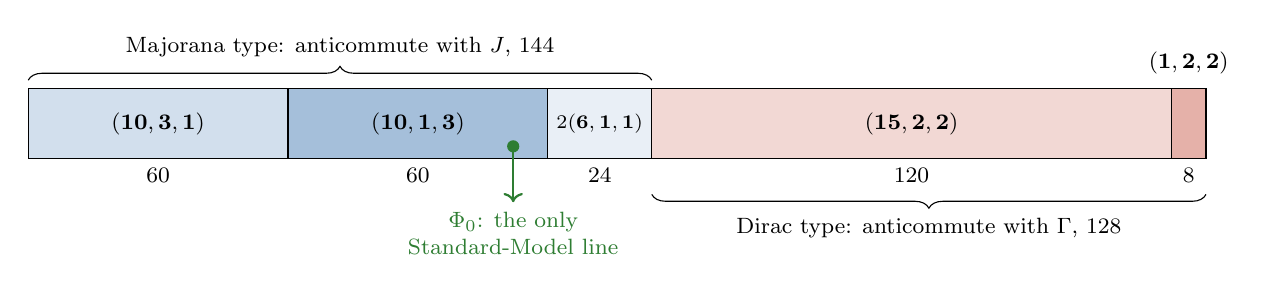
\begin{tikzpicture}[x=0.055cm,y=1cm,font=\footnotesize]
\def\kbar#1#2#3#4#5{\fill[#4] (#1,0) rectangle (#2,0.9); \draw (#1,0) rectangle (#2,0.9); \node at ({(#1+#2)/2},0.45) {#3}; \node[below,font=\footnotesize] at ({(#1+#2)/2},0) {#5};}
\kbar{0}{60}{$(\mathbf{10},\mathbf3,\mathbf1)$}{tcol!20}{$60$}
\kbar{60}{120}{$(\mathbf{10},\mathbf1,\mathbf3)$}{tcol!40}{$60$}
\kbar{120}{144}{\scriptsize$2(\mathbf6,\mathbf1,\mathbf1)$}{tcol!10}{$24$}
\kbar{144}{264}{$(\mathbf{15},\mathbf2,\mathbf2)$}{scol!20}{$120$}
\kbar{264}{272}{}{scol!40}{$8$}
\node[anchor=south,font=\footnotesize] at (268,0.95) {$(\mathbf1,\mathbf2,\mathbf2)$};
\draw[decorate,decoration={brace,amplitude=5pt}] (0,1.0) -- node[above=5pt] {Majorana type: anticommute with $J$, $144$} (144,1.0);
\draw[decorate,decoration={brace,amplitude=5pt,mirror}] (144,-0.45) -- node[below=5pt] {Dirac type: anticommute with $\Gamma$, $128$} (272,-0.45);
\fill[gcol] (112,0.16) circle (2.2pt);
\draw[gcol,thick,->] (112,0.16) -- (112,-0.55) node[below,align=center,font=\footnotesize] {$\Phi_0$: the only\\ Standard-Model line};
\end{tikzpicture}
\caption{The $272$-dimensional space of Lorentz-invariant mass kernels of the chiral block (\cref{thm:kernelspace}), drawn to scale. The
Standard-Model invariant kernels form a single complex line, the right-handed neutrino Majorana kernel $\Phi_0$, inside $(\mathbf{10},\mathbf1,\mathbf3)$.}
\label{fig:kernels}
\end{figure}

The complex dimension of $\Kc$ is $136=\dim\mathrm{Sym}^2(\C^{16})$: a Lorentz-invariant mass term of sixteen Weyl fermions is a complex
symmetric $16\times16$ matrix. In the language of $\so{10}$, $\mathrm{Sym}^2(\mathbf{16})=\mathbf{10}\oplus\mathbf{126}$ \cite{Slansky}, and the
decomposition (ii) is the Pati--Salam branching of $\mathbf{10}\oplus\mathbf{126}$; the $(\mathbf{10},\mathbf1,\mathbf3)\subset\mathbf{126}$ is the field which, in
minimal left--right and Pati--Salam models, gives the right-handed neutrino a Majorana mass \cite{MohapatraSenjanovic80,MohapatraSenjanovic81}.
Here this content has been obtained from \cref{def:kernel}, with only the Pati--Salam algebra acting. The only component containing a
Standard-Model singlet is $(\mathbf{10},\mathbf1,\mathbf3)$: the colour-singlet parts of $(\mathbf{10},\mathbf3,\mathbf1)$, $(\mathbf{15},\mathbf2,\mathbf2)$ and $(\mathbf1,\mathbf2,\mathbf2)$ carry
$Y=\pm1$ or $\pm\tfrac12$, and $(\mathbf6,\mathbf1,\mathbf1)$ has none.

\begin{theorem}[Symmetric criticality]
\label{thm:symcrit}
Let $V:\Kc\to\R$ be smooth and invariant under the Pati--Salam group acting by $M\mapsto gMg^{-1}$. Then for every $r\in\R$
\[
\nabla V(r\Phi_0)=\frac1{\langle\Phi_0,\Phi_0\rangle}\,\frac{d}{dr}V(r\Phi_0)\,\Phi_0 ,
\]
so $r\Phi_0$ is a critical point of $V$ if and only if $r$ is a critical point of $r\mapsto V(r\Phi_0)$.
\end{theorem}

\begin{proof}
The action is orthogonal. If $h$ fixes $x=r\Phi_0$, invariance gives $h\nabla V(x)=\nabla V(x)$, so $\nabla V(x)$ is fixed by the Standard-Model
group and lies in $\operatorname{span}\{\Phi_0,J\Phi_0\}$. Since $J\Phi_0=[t^R_3,\Phi_0]$ is tangent to the orbit, $\langle\nabla V(x),J\Phi_0\rangle=0$, and
only the radial component remains.
\end{proof}

This is Michel's theorem on critical orbits \cite{Michel71}, the principle of symmetric criticality \cite{Palais79}. Its content here is that no
invariant coupling on the whole kernel space can generate a tadpole for any other component along $\Phi_0$. It says nothing about the second
variation or about other minima, which are the subject of \cref{sec:selection}.

\subsection{The kernel field and its action}

\begin{assumption}
\label{ass:field}
The kernels are the values of a scalar field $\Phi(x)\in\Kc$ with kinetic term $\tfrac12\langle D_\mu\Phi,D^\mu\Phi\rangle$ and a potential $V(\Phi)$
invariant under the gauge algebra, and a single Yukawa coupling $y$ in \eqref{eq:Saction}. The overall normalisation of the kinetic term is a
convention; its use of one trace form on all of $\Kc$, the single coupling $y$ and the form of $V$ are choices, restricted below only by symmetry.
\end{assumption}

With a real Grassmann field $\psi(x)\in V_*$, a gauge field $A_\mu$ with values in an algebra $\mathfrak g$ of antisymmetric operators, the kinetic
kernels $K^\mu=P_*\gamma^0\gamma^\mu P_*$ (symmetric, $K^0=\id$ on $V_*$) and the module metric $G_{ab}=\Tr(T_a^{\!\top}T_b)/512$, take
\begin{equation}
\label{eq:Saction}
S=\int d^4x\Bigl[\tfrac12\psi^{\!\top}K^\mu D_\mu\psi+\tfrac y2\psi^{\!\top}\Phi\psi+\tfrac12\langle D_\mu\Phi,D^\mu\Phi\rangle-V(\Phi)-\tfrac14G_{ab}F^a_{\mu\nu}F^{b\mu\nu}\Bigr],
\end{equation}
with $D_\mu\psi=\partial_\mu\psi+A_\mu\psi$ and $D_\mu\Phi=\partial_\mu\Phi+[A_\mu,\Phi]$. Every term is Lorentz invariant by \cref{def:kernel}, and gauge
invariant for any $\mathfrak g$ inside the $23$-dimensional faithful algebra of the block. The module metric is $1$ on the colour bivectors and
$\tfrac18$ on $t^L$ and $t^R$.

\begin{proposition}[Fermion number]
\label{prop:fermionnumber}
$J$ commutes with the kinetic kernels and with the $21$ Pati--Salam generators. The transformation $\psi\mapsto e^{\theta J}\psi$,
$\Phi\mapsto e^{\theta J}\Phi e^{-\theta J}$, $A\mapsto A$ leaves every term of \eqref{eq:Saction} except $V$ invariant; on $\Kc$ it acts as
$\Phi\mapsto e^{2\theta J}\Phi$ on Majorana-type kernels and trivially on Dirac-type ones. In the complex structure $J$ each of the sixteen Weyl
fermions has charge $1$, so this is the fermion number $F=3B+L$, and $4B=F+(\BmL)$.
\end{proposition}

By \cref{prop:PSanom} the two central directions $J$ and $J\Gamma$ are anomalous on this matter, so the gauge algebra can be any anomaly-free
subalgebra of the $23$, and $\su4\oplus\su2_L\oplus\su2_R$ is the largest one containing Pati--Salam. A gauge field coupled to an anomalous current
makes the quantum theory inconsistent \cite{GrossJackiw72,BouchiatIliopoulosMeyer72}, which is why the central directions carry no gauge
field; they remain global symmetries. In the vacuum $r\Phi_0$ the stabiliser among the $23$ generators is fourteen-dimensional: the twelve
Standard-Model generators together with $J+\tfrac13H$ and $J-J\Gamma$, whose charges are $1+(\BmL)=4B$ and $1-\Gamma$, baryon number and twice
the left-handed fermion number, both global.

\begin{proposition}[The coupled field equations]
\label{prop:coupled3}
The Euler--Lagrange equations of \eqref{eq:Saction} are
\[
K^\mu D_\mu\psi+y\Phi\psi=0,\qquad D_\mu D^\mu\Phi+\nabla V(\Phi)-\tfrac y2\Pi_\Kc(\psi\psi^{\!\top})=0,\qquad G_{ab}D_\nu F^{b\nu\mu}=-\bigl(j^\mu_a(\psi)+j^\mu_a(\Phi)\bigr),
\]
with $\Pi_\Kc$ the orthogonal projection onto $\Kc$. At constant $\Phi=r\Phi_0$, $\psi=0$, $A=0$ the first and third hold identically and the second
reduces to $\tfrac{d}{dr}V(r\Phi_0)=0$ by \cref{thm:symcrit}. The same holds with $V$ replaced by the effective potential, which is again
Pati--Salam invariant; at one loop
\begin{equation}
\label{eq:V1}
V_1=\frac1{64\pi^2}\,\mathrm{STr}\Bigl[\mathcal M^4\Bigl(\ln\frac{\mathcal M^2}{\mu_R^2}-c\Bigr)\Bigr],\qquad
\mathrm{STr}=\textstyle\sum_{\rm scalars}+3\sum_{\rm vectors}-2\sum_{\rm Weyl},
\end{equation}
the fermion term being the determinant of the Dirac operator of the first equation \cite{ColemanWeinberg73,Jackiw74}; at stationary points it
does not depend on the gauge fixing \cite{Nielsen75}.
\end{proposition}

The fermions, classically zero, act on the vacuum only through the effective potential, and the matter content enters through the Yukawa
coupling $y$. That there is one such coupling is part of \cref{ass:field}, not a consequence of calling $\Phi$ one field: $\Phi$ is reducible under the
Pati--Salam algebra, and symmetry alone allows an independent Yukawa coupling and an independent kinetic normalisation for each of its five irreducible
components, with a mixing between the two copies of $(\mathbf6,\mathbf1,\mathbf1)$. The same is true of the common gauge coupling of $\su4$ and $\su2_R$ used in
\cref{sec:selection}. In the vacuum the block Hamiltonian is $H(p)=p_iK^i+iy\,r\,\Phi_0$; since $\{K^i,K^j\}=2\delta^{ij}$,
$\{K^i,\Phi_0\}=0$ and $-\Phi_0^2=P_\nu$,
\[
H(p)^2=|p|^2+y^2r^2P_\nu :
\]
one Majorana fermion, the right-handed neutrino, with four real components and mass $|y|r$, and sixty massless real components.

\Cref{thm:symcrit} settles stationarity for the whole coupled quantum system along $\Phi_0$. Which orbit is the \emph{minimum} is decided by the
couplings, and that is the subject of the next section. A non-negative second variation on the $(\mathbf{10},\mathbf1,\mathbf3)$ directions alone does not
imply it on all of $\Kc$: fluctuations outside $(\mathbf{10},\mathbf1,\mathbf3)$ with the Standard-Model quantum numbers of $(\mathbf{10},\mathbf1,\mathbf3)$ fluctuations can
mix with them, and \cref{sec:fullK} exhibits such a mixing.

\section{Selecting the Standard-Model orbit}
\label{sec:selection}

The Standard-Model line $\Phi_0$ lies in the $(\mathbf{10},\mathbf1,\mathbf3)$ component, which is small enough to be analysed completely. We first classify
the renormalizable potential on that component and give sufficient and necessary conditions for $\Phi_0$ to be its global minimum; then we add the gauge
and matter fluctuations;
and finally we return to the whole of $\Kc$.

\subsection{The tensor model}

Let $\su4\oplus\su2_R$ act on $\C^8=\C^4\otimes\C^2$ by Hermitian generators normalised by $\Tr T_aT_b=\tfrac12\delta_{ab}$ in the fundamental, and on complex
symmetric $8\times8$ matrices by $S\mapsto USU^{\!\top}$. The subspace
\[
\mathcal T=\mathrm{Sym}^2(\C^4)\otimes\mathrm{Sym}^2(\C^2)\subset\mathrm{Sym}^2(\C^8),\qquad \dim_\C\mathcal T=30,\qquad |S|^2=\Tr S^\dagger S,
\]
is invariant and irreducible, isomorphic to $(\mathbf{10},\mathbf1,\mathbf3)$. With $e_1,\dots,e_4$ and $e_\pm$ the standard bases of $\C^4$ and $\C^2$, $\BmL=\operatorname{diag}(\tfrac13,\tfrac13,\tfrac13,-1)$
and $T^R_3=\operatorname{diag}(\tfrac12,-\tfrac12)$, the vectors $e_i\otimes e_+$, $e_4\otimes e_+$, $e_i\otimes e_-$, $e_4\otimes e_-$ ($i\le3$) carry $Y=\tfrac23,0,-\tfrac13,-1$:
they are $u_R$, $\nu_R$, $d_R$, $e_R$, and a component of $S$ is a pair of them. Put $u_0=e_4\otimes e_+$ and $S_0=u_0u_0^{\!\top}$.

\begin{proposition}[From kernels to tensors]
\label{prop:tensor}
The component $\Kc_{(\mathbf{10},\mathbf1,\mathbf3)}$ is $J$-invariant of real dimension $60$, and with $J$ as complex structure it is isomorphic to $\mathcal T$ by a
Pati--Salam-equivariant $\iota$ with $\Tr\Phi^{\!\top}\Phi=4|\iota(\Phi)|^2$, unique up to a phase, with $\iota(\Phi_0)=e^{i\varphi}S_0$. For
$S=\iota(\Phi)$, $\Phi^{\!\top}\Phi$ is supported on the $\Gamma=+1$ half and has the spectrum of $S^\dagger S$, each eigenvalue four times, so
\[
N:=\Tr\Phi^{\!\top}\Phi=4|S|^2,\qquad Q:=\Tr(\Phi^{\!\top}\Phi)^2=4\Tr(S^\dagger S)^2,\qquad \frac Q{N^2}=\frac14\,\frac{\Tr(S^\dagger S)^2}{|S|^4}.
\]
\end{proposition}

Let $P_1,\dots,P_5$ be the orthogonal projectors of $\mathrm{Sym}^2\mathcal T$ onto its five irreducible components
\[
(\mathbf{35},\mathbf5)\oplus(\mathbf{35},\mathbf1)\oplus(\mathbf{20}',\mathbf5)\oplus(\mathbf{20}',\mathbf1)\oplus(\mathbf{45},\mathbf3),\qquad 175+35+100+20+135=465,
\]
and put $I_k(S)=\langle S\otimes S,P_k(S\otimes S)\rangle\ge0$, so that $\sum_kI_k=|S|^4$.

\begin{theorem}[The renormalizable potential of $(\mathbf{10},\mathbf1,\mathbf3)$]
\label{thm:potential}
The most general renormalizable invariant potential on $\mathcal T$ is
\begin{equation}
\label{eq:Vgeneral}
V(S)=-\mu^2|S|^2+\sum_{k=1}^5\lambda_kI_k(S)+\kappa\,\mathcal D(S)+\bar\kappa\,\overline{\mathcal D(S)},\qquad \lambda_k\in\R,\ \kappa\in\C,
\end{equation}
where the holomorphic quartic is
\[
\mathcal D(S)=\tfrac1{24}\,\epsilon^{abcd}\epsilon^{efgh}P_{ab,ef}(S)P_{cd,gh}(S),\qquad P_{ab,ef}(S)=\varepsilon_{su}\varepsilon_{tv}S_{as,et}S_{bu,fv},
\]
with colour indices $a,\dots,h$ and $\su2_R$ indices $s,t,u,v$. There is no invariant cubic. Moreover:
\begin{enumerate}[label=(\roman*),leftmargin=2.2em]
\item $\mathcal D(e^{i\theta}S)=e^{4i\theta}\mathcal D(S)$, every $I_k$ is phase invariant, and $\mathcal D$ is not a combination of the $I_k$.
\item $\mathcal D$ depends on $S$ only through the $(\mathbf{20}',\mathbf1)$ component of $S\otimes S$, and $|\mathcal D(S)|\le\tfrac38I_4(S)$, with equality at
$S=\id_4\otimes\id_2$.
\item Under fermion number $S\mapsto e^{2i\theta}S$, so the $I_k$ are invariant and $\mathcal D\mapsto e^{8i\theta}\mathcal D$: \eqref{eq:Vgeneral} is invariant
under fermion number if and only if $\kappa=0$. $\mathcal D$ has $\BmL=0$ and fermion number $8$, hence baryon number $2$.
\end{enumerate}
\end{theorem}

The trivial representation occurs in $\mathcal T\otimes\bar{\mathcal T}$, $\mathrm{Sym}^2\mathcal T$, $\mathrm{Sym}^3\mathcal T$, $\mathrm{Sym}^2\mathcal T\otimes\bar{\mathcal T}$,
$\mathrm{Sym}^4\mathcal T$, $\mathrm{Sym}^3\mathcal T\otimes\bar{\mathcal T}$ and $\mathrm{Sym}^2\mathcal T\otimes\mathrm{Sym}^2\bar{\mathcal T}$ with multiplicities $1,0,0,0,1,0,5$,
which is the content of the theorem. The phase of $\kappa$ can be removed by $S\mapsto e^{i\alpha}S$, so only $|\kappa|$ matters. The contraction of four
$(\mathbf{10},\mathbf1,\mathbf3)$ fields with two $SU(4)$ $\epsilon$ tensors is the baryon-number-violating coupling of Pati--Salam models through which diquark
components mediate neutron--antineutron oscillation \cite{MohapatraMarshak80,ChackoMohapatra99}.

Two lemmas organise the quartics. The first is the recoupling identity $\Tr(S^\dagger S)^2=I_1-\tfrac12I_2-\tfrac12I_3+\tfrac14I_4+0\cdot I_5$, obtained from
Schur--Weyl duality on $(\C^4)^{\otimes4}\otimes(\C^2)^{\otimes4}$. The second characterises the orbit of $S_0$.

\begin{lemma}[The highest-weight orbit]
\label{lem:hw}
For $S\in\mathcal T\setminus0$ the following are equivalent: $S\otimes S$ lies in $(\mathbf{35},\mathbf5)$; $\Tr(S^\dagger S)^2=|S|^4$; $\operatorname{rank}S=1$;
$S=(a\otimes b)(a\otimes b)^{\!\top}$ with $a\in\C^4$, $b\in\C^2$; $S$ lies on the orbit $\mathcal O_{\rm hw}$ of $\C^\times S_0$.
\end{lemma}

This is the Kostant--Lichtenstein description of the highest-weight orbit by quadrics \cite{Lichtenstein82}. On $\mathcal O_{\rm hw}$ the colour factor of $S$
has rank one, so $\mathcal D$ vanishes there; more precisely $\mathcal D$ and its first and second derivatives vanish at $S_0$, and
\[
\mathcal D(s_0S_0+\delta)=s_0\Bigl(\tfrac13\epsilon_{ijk}\epsilon_{lmn}U_{il}D_{jm}D_{kn}-\tfrac1{12}\epsilon_{ijk}\epsilon_{lmn}M_{il}M_{jm}D_{kn}\Bigr)+\mathcal D(\delta),
\]
with $U$, $M$, $D$ the symmetric $3\times3$ matrices of the colour sextets $u_Ru_R$, $u_Rd_R$, $d_Rd_R$. In the vacuum the holomorphic quartic contributes
nothing to the masses and produces the cubic couplings $\kappa v\,\epsilon\epsilon\,\Delta_{uu}\Delta_{dd}\Delta_{dd}$ and $\kappa v\,\epsilon\epsilon\,\Delta_{ud}\Delta_{ud}\Delta_{dd}$ of
diquarks of hypercharges $\tfrac43,\tfrac13,-\tfrac23$, each of baryon number two. With the Yukawa couplings of the diquarks to quark pairs, here the
single coupling $y$ of \eqref{eq:Saction}, the vertex closes into a six-quark $\Delta B=2$ operator, the Pati--Salam mechanism of neutron--antineutron
oscillation; the present limits on the oscillation time are $8.6\times10^7$\,s for free neutrons \cite{BaldoCeolin94} and $4.7\times10^8$\,s from
neutrons bound in oxygen \cite{SuperK21}.

\subsection{Where the Standard-Model orbit is the global minimum}

Number the components $k=1,\dots,5$ as above, put $f_k(S)=I_k(S)/|S|^4$ (so $f_k\ge0$, $\sum f_k=1$), $d(S)=|\mathcal D(S)|/|S|^4$, and
\[
\Delta_k=\lambda_k-\lambda_1\ (k\ge2),\qquad \Lambda(S)=\sum_k\lambda_kf_k(S)=\lambda_1+\sum_{k\ge2}\Delta_kf_k(S),\qquad \Lambda_\kappa(S)=\Lambda(S)-2|\kappa|\,d(S).
\]
For a unit vector $\hat S$, $\min_\varphi V(re^{i\varphi}\hat S)=-\mu^2r^2+\Lambda_\kappa(\hat S)r^4$, because the $I_k$ do not depend on the phase and
$2\Re(\kappa e^{4i\varphi}\mathcal D(\hat S))$ reaches $-2|\kappa||\mathcal D(\hat S)|$. With $\mu^2>0$ the potential is bounded below iff $\Lambda_\kappa>0$ on the unit
sphere, the minimum along a ray is $-\mu^4/(4\Lambda_\kappa)$, and the vacuum is the configuration of smallest $\Lambda_\kappa$.

\begin{theorem}[Selection without the holomorphic quartic]
\label{thm:select0}
Let $\kappa=0$, $\mu^2>0$, $\lambda_1>0$ and $\Delta_2,\dots,\Delta_5>0$. The global minima of \eqref{eq:Vgeneral} are exactly the points of $\mathcal O_{\rm hw}$ with
$|S|^2=\mu^2/(2\lambda_1)$, with $V_{\min}=-\mu^4/(4\lambda_1)$. They form one orbit of real dimension nine, and the stabiliser of each point is conjugate to
$\su3\oplus\uu1_Y$ inside $\su4\oplus\su2_R$ with $Y=T^R_3+\tfrac12(\BmL)$; together with $\su2_L$, which acts trivially on $(\mathbf{10},\mathbf1,\mathbf3)$, this is the
Standard-Model algebra.
\end{theorem}

\begin{proof}
$\Lambda\ge\lambda_1$, with equality iff $f_2=\dots=f_5=0$, that is iff $S\in\mathcal O_{\rm hw}$ by \cref{lem:hw}; the unit-norm part of $\mathcal O_{\rm hw}$ is a single
orbit, of dimension $18-9$.
\end{proof}

The unbroken $\uu1$ is an output, computed as the stabiliser: the weights of the vacuum, not a choice of embedding, fix the hypercharge. This is the
vacuum of Pati--Salam and left--right models with a $(\mathbf{10},\mathbf1,\mathbf3)$ field \cite{PatiSalam,MohapatraSenjanovic81}; the theorem says for which couplings
the dynamics chooses it.

\begin{theorem}[Selection with the holomorphic quartic]
\label{thm:selectk}
Let $\mu^2>0$ and $\kappa\in\C$.
\begin{enumerate}[label=(\alph*),leftmargin=2.2em]
\item If $\lambda_1,\lambda_2,\lambda_3,\lambda_5>0$ and $\lambda_4>\tfrac34|\kappa|$, the potential is bounded below; if it is bounded below then $\lambda_1>0$ and
$2\lambda_1+\lambda_2+2\lambda_3+\lambda_4>\tfrac34|\kappa|$.
\item If $\lambda_1>0$, $\Delta_2,\Delta_3,\Delta_5>0$ and $\Delta_4>\tfrac34|\kappa|$, the global minima are exactly the points of $\mathcal O_{\rm hw}$ with
$|S|^2=\mu^2/(2\lambda_1)$.
\item If those points are global minima, then $\Delta_2\ge0$, $\Delta_3\ge0$, $2\Delta_2+2\Delta_3+4\Delta_4+9\Delta_5\ge0$ and
$\Delta_2+2\Delta_3+\Delta_4\ge\tfrac34|\kappa|$.
\item The second variation at the Standard-Model orbit does not depend on $\kappa$.
\end{enumerate}
\end{theorem}

At the benchmark couplings $\lambda=(1,1.7,2.3,3.1,2.9)$ the bounds read: $\tfrac43\Delta_4=2.8$, sufficient for selection; $\tfrac43(\Delta_2+2\Delta_3+\Delta_4)=7.2$,
necessary for selection and equal to the computed threshold; $\tfrac43\lambda_4=4.13$, sufficient for boundedness; and $\tfrac43(2\lambda_1+\lambda_2+2\lambda_3+\lambda_4)=15.2$,
necessary for boundedness. Gradient flows confirm the transition at $|\kappa|=7.2$: from random starts the flow reaches the Standard-Model orbit for every
$|\kappa|$, as it must, since the orbit is always a local minimum, but for $6\le|\kappa|\le7.5$ one of two starts ends on the orbit of $\id_4\otimes\id_2$, which is
the higher of the two minima for $|\kappa|\le7$ and the lower for $|\kappa|\ge7.5$: at the benchmark,
$f(\id_4\otimes\id_2)=(\tfrac13,\tfrac16,\tfrac13,\tfrac16,0)$ and $d(\id_4\otimes\id_2)=\tfrac1{16}$, so
$\Lambda_\kappa(\id_4\otimes\id_2)-\Lambda_\kappa(S_0)=0.9-\tfrac18|\kappa|$, which changes sign at $|\kappa|=7.2$.

\begin{theorem}[Second variation at the Standard-Model orbit]
\label{thm:secondvar}
At $S_v=vS_0$ the sixty real fluctuations split into $SU(3)\times U(1)_Y$ multiplets, each with one mass:
\begin{center}
\small
\begin{tabular}{@{}llccl@{}}
\toprule
pair & $SU(3)_Y$ & $\dim_\R$ & $m^2/v^2$ & role\\
\midrule
$\nu_R\nu_R$ (modulus) & $1_0$ & $1$ & $4\lambda_1$ & radial\\
$\nu_R\nu_R$ (phase), $\nu_Re_R$, $u_R\nu_R$ & $1_0$, $1_{-1}$, $3_{2/3}$ & $1+2+6$ & $0$ & eaten\\
$e_Re_R$ & $1_{-2}$ & $2$ & $\tfrac43\Delta_2$ & $\Delta_{ee}$\\
$u_Re_R+d_R\nu_R$ & $3_{-1/3}$ & $6$ & $\Delta_5$ & $\Delta_{ue}$\\
$d_Re_R$ & $3_{-4/3}$ & $6$ & $\tfrac23\Delta_2+\Delta_5$ & $\Delta_{de}$\\
$u_Ru_R$ & $6_{4/3}$ & $12$ & $\tfrac43\Delta_3$ & $\Delta_{uu}$\\
$u_Rd_R$ & $6_{1/3}$ & $12$ & $\tfrac23\Delta_3+\Delta_5$ & $\Delta_{ud}$\\
$d_Rd_R$ & $6_{-2/3}$ & $12$ & $\tfrac49\Delta_2+\tfrac29\Delta_3+\tfrac49\Delta_4+\Delta_5$ & $\Delta_{dd}$\\
\bottomrule
\end{tabular}
\end{center}
Consequently $S_v$ is a non-degenerate local minimum on $\mathcal T$ iff $\lambda_1,\Delta_2,\Delta_3,\Delta_5>0$ and $2\Delta_2+2\Delta_3+4\Delta_4+9\Delta_5>0$, a region that
strictly contains the cone of \cref{thm:select0}; and, independently of the couplings,
\begin{equation}
\label{eq:sumrules}
m_{de}^2=m_{ue}^2+\tfrac12m_{ee}^2,\qquad m_{ud}^2=m_{ue}^2+\tfrac12m_{uu}^2 .
\end{equation}
\end{theorem}

\begin{example}[Checking a sum rule]
\label{ex:sumrule}
At the benchmark $\lambda=(1,1.7,2.3,3.1,2.9)$ one has $\Delta=(0.7,1.3,2.1,1.9)$, so in units of $v^2$: $m_{ee}^2=\tfrac43\cdot0.7=0.9\overline3$,
$m_{ue}^2=1.9$, $m_{de}^2=\tfrac23\cdot0.7+1.9=2.3\overline6$, and indeed $1.9+\tfrac12\cdot0.9\overline3=2.3\overline6$. Likewise $m_{uu}^2=\tfrac43\cdot1.3=1.7\overline3$
and $m_{ud}^2=\tfrac23\cdot1.3+1.9=2.7\overline6=1.9+\tfrac12\cdot1.7\overline3$. The full $60\times60$ mass matrix at these couplings and $\mu^2=2$ has the
predicted spectrum to $4\times10^{-15}$.
\end{example}

The colour-sextet components $\Delta_{uu},\Delta_{ud},\Delta_{dd}$ are the diquarks just met, and $\Delta_{ee}$ is the doubly charged scalar of left--right models.
The sum rules \eqref{eq:sumrules} hold for the most general renormalizable potential of a single $(\mathbf{10},\mathbf1,\mathbf3)$, with or without $\kappa$. When one of the
bounds $\Delta_2,\Delta_3,\Delta_5>0$ fails, gradient flows end on configurations of lower energy that break electric charge or colour: the configuration
$(e_4e_4)(e_+e_-)$, for instance, keeps colour, but its unbroken abelian factor is $T^R_3$ instead of $Y$.

\subsection{The trace potential}

The kernel field carries two quartic invariants that do not refer to the Pati--Salam decomposition at all, $N^2$ and $Q=\Tr(\Phi^{\!\top}\Phi)^2$; they are
invariant under every orthogonal change of basis of the block that preserves $\Kc$, in particular under fermion number, so the trace potential has
$\kappa=0$.

\begin{theorem}[The trace potential on $(\mathbf{10},\mathbf1,\mathbf3)$]
\label{thm:tracepot}
Let $V_{\rm tr}=-\mu^2N+\alpha N^2+\beta Q$ with $\mu^2>0$. In the variables of \cref{thm:potential}, $\lambda_k=16\alpha+4\beta a_k$ with $a=(1,-\tfrac12,-\tfrac12,\tfrac14,0)$,
so $(\Delta_2,\Delta_3,\Delta_4,\Delta_5)=-4\beta\,(\tfrac32,\tfrac32,\tfrac34,1)$. If $\beta<0$ and $\alpha+\tfrac14\beta>0$, the global minimum is the Standard-Model orbit; if
$\beta>0$ and $\alpha+\tfrac1{32}\beta>0$, the minima are the $S$ with $S^\dagger S=\tfrac18|S|^2\id_8$, and every one of them breaks colour; if $\beta=0$ the potential is
$O(60)$-symmetric and the orbit is chosen by fluctuations.
\end{theorem}

$Q/N^2$ measures how concentrated the Majorana mass matrix is: it equals $\tfrac14$ when one fermion carries all of it and $\tfrac1{32}$ when the eight
right-handed fermions share it equally. A negative $\beta$ rewards concentration on a single line, and the only line on which the dynamics can concentrate
without breaking colour is $\nu_R$. The Standard-Model vacuum is the concentrated phase of the Majorana mass, which is the three-constituent form of
the Majorana phase of \cref{thm:twophases}.

\subsection{The fluctuations decide: back-reaction on \texorpdfstring{$(\mathbf{10},\mathbf1,\mathbf3)$}{(10,1,3)}}

Take the tree potential degenerate on $(\mathbf{10},\mathbf1,\mathbf3)$, $\lambda_1=\dots=\lambda_5$ and $\kappa=0$, the case $\beta=0$. Every unit direction of $\mathcal T$ is then a
tree-level minimum, and the orbit is chosen by the one-loop potential \eqref{eq:V1}. Gauge and Yukawa interactions respect fermion number, so they do not
generate $\kappa$ in perturbation theory. Write $L=\ln(\Lambda_{\rm UV}^2/v^2)$. The orbit-dependent part of the leading logarithm is
\[
\delta V=\frac L{64\pi^2}\Bigl[2\sum_{\rm fam}\Tr(M_F^\dagger M_F)^2-3\Tr M_V^4-\Tr M_S^4\Bigr],
\]
where for the degenerate tree potential $\Tr M_S^4$ depends on $|S|$ only. Here and in \cref{sec:fullK} the field is normalised canonically. By
\cref{prop:tensor}, $\Tr\Phi^{\!\top}\Phi=4|\iota(\Phi)|^2$, so the kinetic term of \cref{ass:field} is $\Tr(DS)^\dagger(DS)$ for $S:=\sqrt2\,\iota(\Phi)$, and from
here on $S$ denotes this field and $v=|S|=|\Phi|/\sqrt2=\sqrt2\,r$, the $v$ of \cref{sec:fullK,sec:matter}. In these variables the right-handed neutrino mass
$|y|r$ of \cref{sec:kernels} reads $(|y|/\sqrt2)\,v$, so the $y$ of $M_F=yS$ below is the coupling of \eqref{eq:Saction} divided by $\sqrt2$, while the
coupling $g$ is the same as in \cref{thm:compat}. The vector mass matrix is $(M_V^2)_{ab}=2g^2\Re\Tr(T_aS+ST_a^{\!\top})^\dagger(T_bS+ST_b^{\!\top})$
with one coupling for $\su4$ and $\su2_R$, and the eight right-handed Weyl fermions get the Majorana matrix $M_F=yS$.

\begin{theorem}[One-loop selection on $(\mathbf{10},\mathbf1,\mathbf3)$]
\label{thm:oneloop1013}
At leading logarithm, $\Tr M_V^4=g^4\sum_kc_kI_k$ with $c=(33,3,-3,39,5)$ and $\Tr(M_F^\dagger M_F)^2=y^4\sum_ka_kI_k$, and the fluctuations generate the gaps
\[
\Delta_k=\frac L{64\pi^2}\,g^4\bigl(G_k-x\,F_k\bigr),\qquad G=(90,108,-18,84),\quad F=(3,3,\tfrac32,2),\qquad x=\frac{\sum_{\rm fam}y^4}{g^4}.
\]
Gauge fluctuations favour the Standard-Model orbit in the directions $k=2,3,5$, and matter fluctuations disfavour it in every direction. The Standard-Model
orbit is a non-degenerate local minimum on $\mathcal T$ iff $x<30$, the binding conditions being those of $\Delta_{ee}$ and $\Delta_{dd}$. The configuration $\id_4\otimes\id_2$
has excess $\tfrac L{64\pi^2}g^4(48-\tfrac74x)$ over the Standard-Model orbit, negative for $x>\tfrac{192}7\approx27.43$.
\end{theorem}

At $x=0$ the radiatively generated masses are, in units of $\tfrac L{64\pi^2}g^4v^2$, $m_{ee}^2=120$, $m_{ue}^2=84$, $m_{de}^2=144$, $m_{uu}^2=144$, $m_{ud}^2=156$ and
$m_{dd}^2=120$, which satisfy \eqref{eq:sumrules}; the fifty massive scalars are pseudo-Goldstone bosons of the accidental $O(60)$ symmetry of the tree potential
\cite{Weinberg72,GildenerWeinberg76}. A projected gradient flow on the unit sphere of $\mathcal T$ from random starts finds no configuration below the Standard-Model
orbit for $x\le27$, finds the orbit of $\id_4\otimes\id_2$ as the only competitor, and confirms that its energy crosses zero at $x=192/7$; between $192/7$ and $30$ the
Standard-Model vacuum is metastable on $\mathcal T$. We conjecture that on $\mathcal T$ the Standard-Model orbit is the global minimum of the one-loop potential exactly
for $x<192/7$.

With $M_N=yv$ and $M_{W_R}=gv$, $x=\sum_{\rm fam}(M_N/M_{W_R})^4$; in the couplings of \eqref{eq:Saction} and \cref{thm:compat},
$x=\sum_{\rm fam}y^4/(4g^4)$. Stated in terms of masses, $x$ does not depend on the normalisation. The content of the bound is structural: the Majorana Yukawa coupling, matter's only handle on the
vacuum, pushes towards configurations in which the Majorana mass is shared among several fermions, and the gauge fluctuations hold the Standard-Model orbit only
while the heavy neutrinos are not much heavier than $W_R$.

\subsection{The full kernel space}
\label{sec:fullK}

The general invariant potential on all of $\Kc$ has too many couplings to be classified usefully: the numbers of linearly independent Pati--Salam-invariant
real polynomials of degrees $1,2,3,4$ are $0,18,0,686$, and with fermion number imposed $0,12,0,402$. Two structures do not depend on these couplings.

\begin{proposition}[A left--right involution]
\label{prop:LR}
Let $O=E_1E_7E_8$ restricted to $V_*$. It commutes with $P_*$ and with the rotations, satisfies $O^{\!\top}K^0O=K^0$, $O^{\!\top}K^iO=-K^i$, $O\Gamma O^{\!\top}=-\Gamma$ and
$OJO^{\!\top}=J$, and maps $t^L_i$ to $\pm t^R_i$ and each colour bivector to $\pm$ itself. Hence $\psi(t,\mathbf x)\mapsto O\psi(t,-\mathbf x)$, $\Phi\mapsto O\Phi O^{\!\top}$,
with the corresponding map of the gauge fields, is a symmetry of the kinetic, Yukawa and gauge terms of \eqref{eq:Saction}, and of the trace invariants. The image
$\Phi_0'=O\Phi_0O^{\!\top}$ is a kernel in $(\mathbf{10},\mathbf3,\mathbf1)$ orthogonal to $\Phi_0$, the mirror vacuum of left--right models, and along the great circle
$\hat u(\theta)=\cos\theta\,\hat u_0+\sin\theta\,\hat u_0'$, $Q=\tfrac14-\tfrac18\sin^22\theta$.
\end{proposition}

The Standard-Model vacuum and its mirror are exchanged by a symmetry of the action, so an $O$-invariant potential cannot prefer one of them; the choice between
breaking $\su2_R$ and breaking $\su2_L$ is spontaneous, as in models of spontaneous parity violation \cite{SenjanovicMohapatra75}.

Now take the tree potential degenerate on all of $\Kc$, $V_0=-\mu^2N+\alpha N^2$, invariant under the accidental $O(272)$. For a unit vector $\hat u\in\Kc$ put
\[
\begin{gathered}
Q(\hat u)=\Tr(\hat u^{\!\top}\hat u)^2,\qquad T(\hat u)=\Tr\bigl(G^{-1}K(\hat u)\bigr)^2,\qquad K(\hat u)_{ab}=\langle[t_a,\hat u],[t_b,\hat u]\rangle,\\
E_x(\hat u)=8x\,Q(\hat u)-\tfrac3{16}T(\hat u),
\end{gathered}
\]
with the $21$ Pati--Salam generators $t_a$ and the module metric $G$. The orientation-dependent part of the leading logarithm is then
$\delta V=\tfrac L{64\pi^2}g^4v^4E_x(\Phi/|\Phi|)$ with $v=|\Phi|/\sqrt2$, and at the Standard-Model point $E_x(\hat u_0)=2x-99$.

\begin{theorem}[One-loop second variation on all of $\Kc$]
\label{thm:fullsecond}
Let $H(x)$ be the second variation of $E_x$ at $\hat u_0$ on the $271$-dimensional tangent space of the unit sphere.
\begin{enumerate}[label=(\roman*),leftmargin=2.2em]
\item $H(x)=H_G+xH_F$ with $H_F=-8(\id-\Pi_\nu)$, where $\Pi_\nu$ is the orthogonal projector of rank $32$ onto the kernels that pair $\nu_R$ with a Weyl fermion of the
block. $H_G$ preserves each Pati--Salam component of $\Kc$.
\item With $m^2=\tfrac12\times$(eigenvalue of $H(x)$) in units of $\tfrac L{64\pi^2}g^4v^2$, the $271$ angular modes have the masses of \cref{tab:271}.
\item $H(x)$ is non-negative with kernel exactly the nine Goldstone directions if and only if $x<27$. At $x=27$ the six modes of $\ell_L\ell_L$, the left-handed triplet,
become massless, and for $x>27$ they are tachyonic.
\end{enumerate}
\end{theorem}

\begin{table}[t]
\centering
\footnotesize
\setlength{\tabcolsep}{4pt}
\begin{tabular}{@{}llccl@{}}
\toprule
fermion pair & multiplet & $\dim_\R$ & component & $m^2$\\
\midrule
$\nu_R\nu_R$ (phase), $\nu_Re_R$, $\nu_Ru_R$ & $(1,1)_0,(1,1)_1,(3,1)_{2/3}$ & $1+2+6$ & $(\mathbf{10},\mathbf1,\mathbf3)$ & $0$ (Goldstone)\\
$e_Re_R$ & $(1,1)_2$ & $2$ & $(\mathbf{10},\mathbf1,\mathbf3)$ & $120-4x$\\
$d_Re_R$ & $(3,1)_{4/3}$ & $6$ & $(\mathbf{10},\mathbf1,\mathbf3)$ & $144-4x$\\
$u_Ru_R$ & $(6,1)_{4/3}$ & $12$ & $(\mathbf{10},\mathbf1,\mathbf3)$ & $144-4x$\\
$u_Rd_R$ & $(6,1)_{1/3}$ & $12$ & $(\mathbf{10},\mathbf1,\mathbf3)$ & $156-4x$\\
$d_Rd_R$ & $(6,1)_{2/3}$ & $12$ & $(\mathbf{10},\mathbf1,\mathbf3)$ & $120-4x$\\
$u_Re_R\pm d_R\nu_R$ & $(3,1)_{1/3}$ & $6+6$ & $(\mathbf{10},\mathbf1,\mathbf3)$, $(\mathbf6,\mathbf1,\mathbf1)_R$ & eigenvalues of $M_3$\\
$u_Rd_R$ (antisymmetric) & $(3,1)_{1/3}$ & $6$ & $(\mathbf6,\mathbf1,\mathbf1)_R$ & $180-4x$\\
$u_Le_L-d_L\nu_L$, $u_Ld_L$ & $(3,1)_{1/3}$ & $6+6$ & $(\mathbf6,\mathbf1,\mathbf1)_L$ & $180-4x$\\
$\ell_L\ell_L$ & $(1,3)_1$ & $6$ & $(\mathbf{10},\mathbf3,\mathbf1)$ & $108-4x$\\
$q_L\ell_L$ & $(3,3)_{1/3}$ & $18$ & $(\mathbf{10},\mathbf3,\mathbf1)$ & $156-4x$\\
$q_Lq_L$ & $(6,3)_{1/3}$ & $36$ & $(\mathbf{10},\mathbf3,\mathbf1)$ & $180-4x$\\
$q_L$--$u_R$, $q_L$--$d_R$ (octet) & $(8,2)_{1/2}$ & $64$ & $(\mathbf{15},\mathbf2,\mathbf2)$ & $174-4x$\\
$\ell_L$--$u_R$, $q_L$--$e_R$ & $(3,2)_{7/6}$ & $24$ & $(\mathbf{15},\mathbf2,\mathbf2)$ & $162-4x$\\
$\ell_L$--$d_R$ & $(3,2)_{1/6}$ & $12$ & $(\mathbf{15},\mathbf2,\mathbf2)$ & $114-4x$\\
$q_L$--$\nu_R$ & $(3,2)_{1/6}$ & $12$ & $(\mathbf{15},\mathbf2,\mathbf2)$ & $114$\\
$q_L$--$d_R$, $\ell_L$--$e_R$ (singlets) & $(1,2)_{1/2}$ & $4+4$ & $(\mathbf{15},\mathbf2,\mathbf2)$, $(\mathbf1,\mathbf2,\mathbf2)$ & $138-4x$, $186-4x$\\
$q_L$--$u_R$, $\ell_L$--$\nu_R$ (singlets) & $(1,2)_{1/2}$ & $4+4$ & $(\mathbf{15},\mathbf2,\mathbf2)$, $(\mathbf1,\mathbf2,\mathbf2)$ & eigenvalues of $M_2$\\
\bottomrule
\end{tabular}
\caption{The radiatively generated masses of the $271$ angular modes of the kernel field at the Standard-Model vacuum, in units of $\tfrac L{64\pi^2}g^4v^2$, with
$x=\sum_{\rm fam}(M_N/M_{W_R})^4$ (\cref{thm:fullsecond}). Pairs written $ff'$ are of Majorana type, pairs written $f$--$f'$ of Dirac type; multiplets are given
under $SU(3)\times SU(2)_L$ with $|Y|$. The two mixing matrices are
$M_3=\bigl(\begin{smallmatrix}84-2x&2x\\2x&180-2x\end{smallmatrix}\bigr)$ and $M_2=\bigl(\begin{smallmatrix}138-x&\sqrt3x\\\sqrt3x&186-3x\end{smallmatrix}\bigr)$, with eigenvalues
$132-2x\mp2\sqrt{x^2+576}$ and $162-2x\mp2\sqrt{x^2-12x+144}$.}
\label{tab:271}
\end{table}

Statement (i) is the mechanism by which matter opposes the Standard-Model orbit, now on all of $\Kc$. At fixed $|\Phi|$ the fermion loop $2\sum m_f^4$ is largest when the
whole Majorana mass sits on $\nu_R$; it decreases quadratically along every direction that moves mass onto pairs not containing $\nu_R$ and is stationary along the
directions that pair $\nu_R$ with another fermion. Every mode that does not involve $\nu_R$ therefore has slope $-4$, and the first of them to become massless is the one
with the smallest gauge contribution, the left-handed triplet. The mixing in $M_3$, between the $(\mathbf{10},\mathbf1,\mathbf3)$ mode $u_Re_R+d_R\nu_R$ and the $(\mathbf6,\mathbf1,\mathbf1)_R$
mode $u_Re_R-d_R\nu_R$, is an instance of the mixing announced at the end of \cref{sec:kernels}: it moves the $\Delta_{ue}$ threshold from $42$ to $315/11$. The
thresholds are the zeros of the lowest lines,
\[
x=27\ (\ell_L\ell_L),\qquad x=28.5\ (\ell_L\text{--}d_R),\qquad x=\tfrac{315}{11}\approx28.64\ (M_3),\qquad x=30\ (e_Re_R,\ d_Rd_R),
\]
and \cref{fig:radiative} shows them. Along the great circle of \cref{prop:LR},
\[
E_x(\hat u(\theta))=2x-99+(27-x)\sin^22\theta ,
\]
so for $x>27$ the Standard-Model vacuum descends towards the left--right symmetric configuration $\theta=\pi/4$, where $\nu_R$ and a left-handed lepton carry equal
Majorana masses.

\begin{figure}[t]
\centering
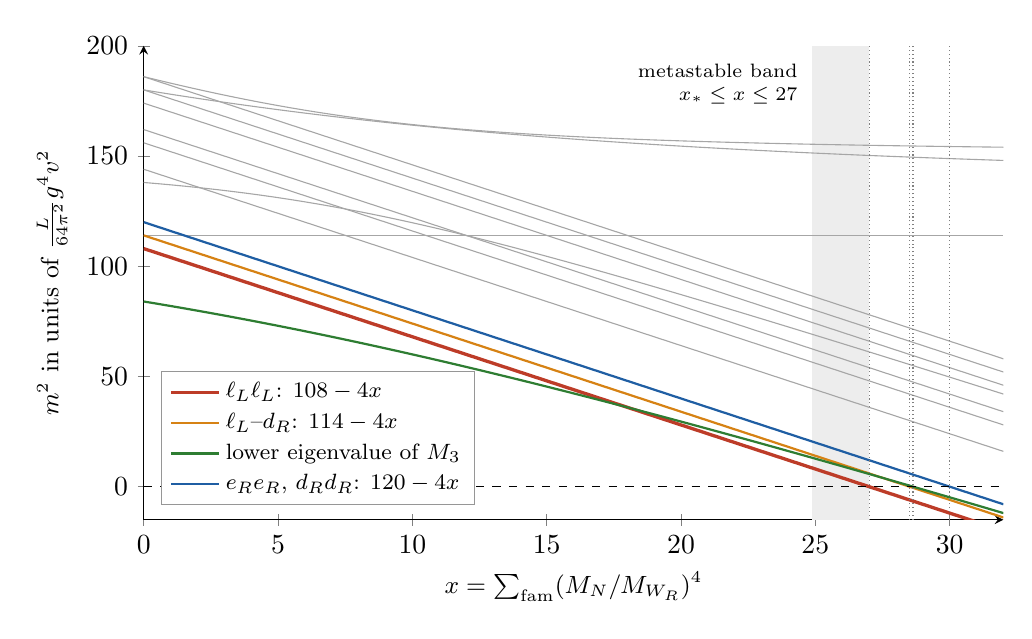
\begin{tikzpicture}
\begin{axis}[width=12.5cm,height=7.6cm,xmin=0,xmax=32,ymin=-15,ymax=200,
  xlabel={$x=\sum_{\rm fam}(M_N/M_{W_R})^4$},ylabel={$m^2$ in units of $\frac{L}{64\pi^2}g^4v^2$},
  axis lines=left,clip=true,xtick={0,5,10,15,20,25,30},ytick={0,50,100,150,200},
  ylabel style={font=\small},xlabel style={font=\small},
  legend style={at={(0.02,0.03)},anchor=south west,font=\footnotesize,fill=white,draw=mgray},legend cell align=left]
\fill[lgray!60] (axis cs:24.884,-15) rectangle (axis cs:27,200);
\addplot[gray!70,thin,forget plot,domain=0:32] {144-4*x};
\addplot[gray!70,thin,forget plot,domain=0:32] {156-4*x};
\addplot[gray!70,thin,forget plot,domain=0:32] {162-4*x};
\addplot[gray!70,thin,forget plot,domain=0:32] {174-4*x};
\addplot[gray!70,thin,forget plot,domain=0:32] {180-4*x};
\addplot[gray!70,thin,forget plot,domain=0:32] {186-4*x};
\addplot[gray!70,thin,forget plot,domain=0:32] {114};
\addplot[gray!70,thin,forget plot,domain=0:32,samples=60] {162-2*x+2*sqrt(x^2-12*x+144)};
\addplot[gray!70,thin,forget plot,domain=0:32,samples=60] {162-2*x-2*sqrt(x^2-12*x+144)};
\addplot[gray!70,thin,forget plot,domain=0:32,samples=60] {132-2*x+2*sqrt(x^2+576)};
\addplot[scol,very thick,domain=0:32] {108-4*x}; \addlegendentry{$\ell_L\ell_L$: $108-4x$}
\addplot[ocol,thick,domain=0:32] {114-4*x}; \addlegendentry{$\ell_L$--$d_R$: $114-4x$}
\addplot[gcol,thick,domain=0:32,samples=80] {132-2*x-2*sqrt(x^2+576)}; \addlegendentry{lower eigenvalue of $M_3$}
\addplot[tcol,thick,domain=0:32] {120-4*x}; \addlegendentry{$e_Re_R$, $d_Rd_R$: $120-4x$}
\draw[black,dashed] (axis cs:0,0) -- (axis cs:32,0);
\draw[gray,densely dotted] (axis cs:27,-15) -- (axis cs:27,200);
\draw[gray,densely dotted] (axis cs:28.5,-15) -- (axis cs:28.5,200);
\draw[gray,densely dotted] (axis cs:28.636,-15) -- (axis cs:28.636,200);
\draw[gray,densely dotted] (axis cs:30,-15) -- (axis cs:30,200);
\node[anchor=north east,font=\scriptsize,align=right] at (axis cs:24.7,196) {metastable band\\ $x_*\le x\le27$};
\end{axis}
\end{tikzpicture}
\caption{Radiatively generated masses of the angular modes of the kernel field at the Standard-Model vacuum (\cref{thm:fullsecond}, \cref{tab:271}). The coloured lines
are the four lowest; they cross zero at $x=27$, $28.5$, $315/11$ and $30$ (dotted). The Standard-Model orbit is a non-degenerate local minimum for $x<27$, and numerically
it is the global minimum for $x<x_*\approx24.884$; in the shaded band it is metastable.}
\label{fig:radiative}
\end{figure}

\begin{proposition}[Random-start minimisation]
\label{prop:randomstart}
$E_x$ was minimised on the unit sphere of $\Kc$ by a quasi-Newton method from Gaussian random starts, with two independent implementations. For $x=0,20,22$ every run
ended at the energy $2x-99$ of the Standard-Model orbit or of its mirror. At $x=25$ a third of the runs ended below it, at a configuration with weight $0.968$ on
$(\mathbf{10},\mathbf1,\mathbf3)$ and $0.032$ on $2(\mathbf6,\mathbf1,\mathbf1)$, whose stabiliser of dimension nine contains $\su2_L$ and projects onto colour with rank six, whereas any
algebra containing $\su3$ projects with rank at least eight: colour is broken. There four right-handed Weyl fermions carry Majorana masses, one of them about twice as heavy
as the other three. Followed in $x$, this minimum crosses the energy of the Standard-Model orbit at $x_*=24.88405$.
\end{proposition}

We conjecture that in the radiative scenario on $\Kc$ the Standard-Model orbit and its mirror are the global minima exactly for $x<x_*$, and that for $x_*<x<27$ the
Standard-Model vacuum is metastable. The competitor again spreads the Majorana mass, now over four right-handed fermions instead of one, which is what the fermion loop
rewards, at the price of breaking colour, which the gauge loop penalises. In terms of masses the local condition and the conjectured global one read
\[
\begin{aligned}
&M_N<27^{1/4}M_{W_R}=2.280\,M_{W_R}\quad\text{and}\quad M_N<2.233\,M_{W_R}&&\text{(one family dominating)},\\
&M_N<9^{1/4}M_{W_R}=1.732\,M_{W_R}\quad\text{and}\quad M_N<1.697\,M_{W_R}&&\text{(three degenerate families)}.
\end{aligned}
\]
They hold under the following restrictions: a tree potential degenerate on $\Kc$ at the matching scale, one loop at leading logarithm, $\kappa=0$, which fermion number
makes automatic, a common gauge coupling for $\su4$ and $\su2_R$, and a single Yukawa coupling for all components of the kernel field (\cref{ass:field}). The masses of
\cref{tab:271} are curvatures of the leading-logarithm effective potential divided by the kinetic norm; pole masses would need the wave-function renormalisation and a
gauge-consistent perturbative expansion, which are not attempted. The bounds are therefore statements about this model and approximation, not bounds on heavy-neutrino
masses outside it. Within it, the result is that gauge fluctuations make the Standard-Model orientation of the
Majorana condensate stable in every direction of the kernel space as long as the heavy neutrinos are not much heavier than $W_R$; beyond that, the local instability is
the condensation of the left-handed triplet, and the configuration that overtakes the Standard-Model orbit globally, at the slightly smaller $x_*$, breaks colour.

\section{Matter in the selected vacuum}
\label{sec:matter}

We return to the vacuum $\Phi=r\Phi_0$, $r\neq0$, with $v=|\Phi|/\sqrt2=\sqrt2\,r$, and ask whether the matter of the block is compatible with
it in the sense stated at the beginning of \cref{sec:kernels}.

\begin{theorem}[Compatibility with matter]
\label{thm:compat}
\begin{enumerate}[label=(\alph*),leftmargin=2.2em]
\item \emph{Unbroken algebra.} Among the $21$ Pati--Salam generators the stabiliser of $\Phi_0$ has dimension $12$ and closes under brackets; its part
orthogonal to $\su3\oplus\su2_L$ is spanned by $t_Y=t^R_3+\tfrac16H$. Among the $23$ generators it has dimension $14$; the two further directions $J+\tfrac13H$
and $J-J\Gamma$ carry the charges $4B$ and $1-\Gamma$ and are global.
\item \emph{Vector bosons.} The matrix $M_{ab}=\langle[t_a,\Phi_0],[t_b,\Phi_0]\rangle/|\Phi_0|^2$, taken relative to the module metric, has eigenvalues $0$ (twelve
times), $4$ (eight times) and $20$ (once), so the squared vector masses are $0$, $g^2v^2$ and $5g^2v^2$. The eight carry $Y=\pm\tfrac23$ (six leptoquarks
$X$) and $\pm1$ (the two $W_R^\pm$); the one at $5g^2v^2$ is neutral, a $Z'$.
\item \emph{Couplings.} In the module trace $|t^L_3|^2=\tfrac18$ and $|t_Y|^2=\tfrac5{24}$, so
\[
\sin^2\theta_W=\frac{|t^L_3|^2}{|t^L_3|^2+|t_Y|^2}=\frac38
\]
at the matching scale, the value of the Pati--Salam and $\so{10}$ embeddings \cite{GeorgiQuinnWeinberg74}.
\item \emph{Dirac operator.} The kinetic kernels are symmetric with $K^0=\id$ and are preserved by the twelve unbroken generators, and $H(p)^2=|p|^2+y^2r^2P_\nu$.
\item \emph{Chirality.} The massless fermions are $(3,2)_{1/6}\oplus(1,2)_{-1/2}$ with $\Gamma=-1$ and $(3,1)_{2/3}\oplus(3,1)_{-1/3}\oplus(1,1)_{-1}$ with $\Gamma=+1$:
the unbroken $\su2_L$ acts on one Lorentz chirality only.
\item \emph{Anomalies.} On the block the $Y^3$, mixed gravitational, $SU(2)^2Y$, $SU(3)^2Y$ and $SU(3)^3$ anomalies vanish, with and without $\nu_R$, and there are
four left-handed $SU(2)$ doublets, an even number \cite{Witten82}.
\end{enumerate}
\end{theorem}

The formula in (c) deserves a line. With one coupling for the whole Pati--Salam algebra, the effective couplings of $t^L_3$ and $t_Y$ are in the ratio of
their norms in the module, $g'^2/g^2=|t^L_3|^2/|t_Y|^2=\tfrac{3/24}{5/24}=\tfrac35$, the familiar normalisation of hypercharge in unified models, and
$\sin^2\theta_W=g'^2/(g^2+g'^2)=\tfrac38$. Every requirement of a matter-compatible vacuum is met at this stage except mass
generation for the charged fermions, which needs the electroweak stage.

\subsection{The electroweak stage and the fermion masses}

Everything in this subsection assumes, in addition, a vacuum value of the bidoublet kernels; their dynamics and their scale are not derived. In the radiative
scenario of \cref{sec:fullK} the colour-singlet doublets have squared masses $138-4x$, $186-4x$ and the eigenvalues of $M_2$, so they sit at the Pati--Salam
scale and a light doublet requires a tuning that we do not derive.

\begin{proposition}[Electroweak stage]
\label{prop:EW}
\begin{enumerate}[label=(\roman*),leftmargin=2.2em]
\item The kernels commuting with $\su3$ and with $Q=T^L_3+Y$ form a $12$-dimensional space: two each in $(\mathbf{10},\mathbf1,\mathbf3)$ and $(\mathbf{10},\mathbf3,\mathbf1)$ and four
each in $(\mathbf{15},\mathbf2,\mathbf2)$ and $(\mathbf1,\mathbf2,\mathbf2)$. In each bidoublet the up-type kernels (no $d,e$ entries) and the down-type kernels (no $u,\nu$ entries)
form two-dimensional spaces.
\item On the charge sectors $u$ ($Q=\tfrac23$), $d$ ($-\tfrac13$), $\nu$ ($0$) and $e$ ($-1$), the $(\mathbf1,\mathbf2,\mathbf2)$ kernels give $m_u=m_\nu^D$ and $m_d=m_e$; the
$(\mathbf{15},\mathbf2,\mathbf2)$ kernels give lepton masses three times the quark masses, with relative sign $-3$ once aligned with a $(\mathbf1,\mathbf2,\mathbf2)$ kernel. For
$\Phi=\kappa_1K_1+\kappa_{15}K_{15}$ of each type,
\[
m_{\rm quark}=|\kappa_1+\kappa_{15}|,\qquad m_{\rm lepton}=|\kappa_1-3\kappa_{15}|,
\]
the Georgi--Jarlskog factor \cite{GeorgiJarlskog79} used in fits of fermion masses with $\mathbf{10}\oplus\mathbf{126}$ \cite{BabuMohapatra93}.
\item With $\Phi=v_R\Phi_0+\kappa K_{1u}$ the neutral sector has singular values $\tfrac12\bigl(\sqrt{v_R^2+4\kappa^2}\mp v_R\bigr)$, each four times: the seesaw pair
\cite{Minkowski77,MohapatraSenjanovic80}, with light mass $\approx\kappa^2/v_R$.
\item For $\Phi=v_R\Phi_0+\kappa_uK_{1u}+\kappa_dK_{1d}$ the stabiliser among the $21$ generators is nine-dimensional, $\su3\oplus\uu1_Q$, and $Q$ annihilates $\Phi$.
\end{enumerate}
\end{proposition}

\begin{example}[An electroweak spectrum]
\label{ex:EWspectrum}
At $(v_R,\kappa_u,\kappa_d)=(20,1,\tfrac12)$ the squared vector masses, for $g=1$ in the units of \cref{thm:compat}(b), are $0$ (nine times), $79.360$ (twice, $W^\pm$),
$127.872$ (once, $Z$), $6400$ (six times), $6480.64$ (twice) and $32032.1$ (once). The ratio $m_W^2/m_Z^2=0.62062$ is close to $\cos^2\theta_W=\tfrac58$, and at
$v_R=200$ it differs from $\tfrac58$ by $-4.4\times10^{-5}$: $\rho=1$ at tree level up to corrections of order $\kappa^2/v_R^2$. In the same vacuum at
$(v_R,\kappa_u,\kappa_d)=(20,3,1)$ the fermion mass eigenspaces are a light Majorana neutrino of mass $(\sqrt{436}-20)/2\approx0.440$ and a heavy one of mass
$(\sqrt{436}+20)/2\approx20.440$, each of real dimension four, the $d$ quarks and the electron with $m_d=m_e=1$, and the $u$ quarks with mass $3$. The
chirality content of the neutral pair is $\langle\Gamma\rangle=\mp\cos2\vartheta$ with $\tan2\vartheta=2\kappa_u/v_R$, which is their mixing, and the Majorana-type part of the full
mass operator is exactly $v_R\Phi_0$: $\nu_L$ acquires its Majorana mass only through the mixing.
\end{example}

What is not obtained here is equally definite: the values of $\kappa_u$ and $\kappa_d$, the potential that would select them together with $v_R$, and the
hierarchy $\kappa\ll v_R$, which in Pati--Salam and left--right models is a tuning of the scalar potential \cite{Gildener76}.

\subsection{What the vacuum does not supply}

The statements of this subsection are impossibility results within explicitly stated algebras of operators. They say where an input enters, not that no
mechanism outside those algebras could replace it.

\begin{proposition}[Chirality is field content]
\label{prop:mirror}
Let $\mathcal A$ be the algebra of operators on $S_3$ generated by the $91$ internal bivectors and $J$. Then $\gamma^0$ commutes with every element of $\mathcal A$ and
with the rotations, anticommutes with $\Gamma$ and the boosts, and maps $V_*$ isometrically onto the orthogonal rank-$64$ subspace $\gamma^0V_*$, on which $\mathcal A$
acts by the same matrices and $\Gamma$ has the opposite sign. Hence every eigenspace of an element of $\mathcal A$ has a mirror image with the same eigenvalue and the
opposite chirality, and no vacuum value of a field with values in $\mathcal A$, nor any function of such values, separates $V_*$ from $\gamma^0V_*$.
\end{proposition}

The block is selected by $X=\Gamma\chi_W$, which contains the spacetime orientation through $\Gamma=J\gamma^0\gamma^1\gamma^2\gamma^3$ and is not in $\mathcal A$. The kernel field
is defined on $V_*$ and presupposes it, so it does not escape the proposition either. The Standard-Model vacuum of \cref{thm:select0} is chiral because the
matter on which it acts already is; this is the arena's form of the fact that a vector-like gauge theory does not generate chirality through its vacuum
\cite{VafaWitten84b}.

\begin{proposition}[Hermitian order parameters keep rank five]
\label{prop:rankfive}
On the spin-up part of the block, the operators commuting with $J$, $\Gamma$ and the twelve Standard-Model generators form a twelve-dimensional algebra whose
symmetric part is six-dimensional: the commutative algebra of the six multiplet projectors $(Q,L,u,d,e,\nu)$, which are pairwise inequivalent. A Hermitian vacuum
value in it commutes with $T^R_3$ and $\BmL$, so its stabiliser contains $\su3\oplus\su2_L\oplus\uu1_{T^R_3}\oplus\uu1_{\BmL}$, of rank five; the Standard-Model algebra, of
rank four, is not the unbroken algebra of such an order parameter.
\end{proposition}

This is the block version of the statement that order parameters of adjoint type do not lower the rank \cite{Li74}. The kernel field escapes it because a
Grassmann bilinear carries charge: $[t^R_3,\Phi_0]=J\Phi_0\neq0$.

\begin{proposition}[Gauge alignment does not see chirality]
\label{prop:alignment}
Consider rank-$64$ projectors $P$ commuting with Lorentz and $J$, with the alignment energy $V(P)=\tfrac1{512}\sum_T\|[T,P]\|^2$ over the $43$ compact internal
bivectors. For $P_*$, $\Pfam$, the colour-singlet lepton projector $P_{\rm lep}$ and the vector-like $Q_v=P_L+\gamma^0P_L\gamma^0$ with $P_L=P_*\tfrac12(\id-\Gamma)$:
\begin{center}
\small
\begin{tabular}{@{}lcccc@{}}
\toprule
 & $P_*$ & $\Pfam$ & $P_{\rm lep}$ & $Q_v$\\
\midrule
$V(P)$ & $5$ & $9$ & $3$ & $5$\\
stabiliser among the $43$ & $23$ & $9$ & $37$ & $25$\\
axial, $P\gamma^0P=0$ & yes & --- & --- & no\\
\bottomrule
\end{tabular}
\end{center}
Alignment prefers $P_{\rm lep}$ to $P_*$, and $V(P_*)=V(P_L)+V(P_R)$ with $V(P_L)=V(P_R)=\tfrac52$ while $V(Q_v)=2V(P_L)=V(P_*)$: the alignment energy does not see
chirality.
\end{proposition}

Vacuum alignment \cite{Peskin80,Preskill81} selects among projectors only by the amount of gauge symmetry they keep; it neither selects the Pati--Salam block nor
distinguishes a chiral block from a vector-like one of the same rank. Finally, with the single Yukawa coupling of \cref{ass:field}, matter opposes the
Standard-Model vacuum: on $(\mathbf{10},\mathbf1,\mathbf3)$ every $F_k$
of \cref{thm:oneloop1013} is positive, and on all of $\Kc$ the Yukawa part of the second variation is $-8x(\id-\Pi_\nu)\le0$. The fermion loop lowers the energy
along every direction that moves Majorana mass away from $\nu_R$ and raises it along none; on its own it would select configurations in which the mass is
spread, which break colour. The matter sector is not the agent that selects the Standard-Model orbit. At one loop the gauge fluctuations are, and they succeed
for $x<27$ locally and, numerically, for $x<x_*$.

\section{Goldstone bosons, antiparticles, baryon number and topology}
\label{sec:goldstone}

The selected vacuum can be examined from four further angles: which of its zero modes are Goldstone bosons and which are eaten; how the discrete
operations that exchange particles and antiparticles act on it; whether the potential protects baryon number; and what topological defects its orbit
supports. Each answer depends on counting the two global central generators $J$ and $J\Gamma$ alongside the $21$ gauged ones.

\subsection{Goldstone bosons}

\begin{proposition}[Goldstone directions attached to the symmetries]
\label{prop:global}
$J$ and $J\Gamma$ are antisymmetric, commute with the kinetic kernels and the $21$ Pati--Salam generators, span the centre of the $23$-dimensional faithful
algebra, are anomalous, and carry no gauge fields. If $V$ is invariant under all $23$ generators and $\Phi$ is stationary, the tangent space of the $23$-orbit
lies in the kernel of the Hessian; the gauge bosons eat the tangents of the $21$-orbit, whose dimension is the rank of the vector mass matrix, and
\[
\#\{\text{symmetry-generated Goldstone directions not eaten}\}=\dim(23\text{-orbit})-\dim(21\text{-orbit}).
\]
\end{proposition}

The count is classical, and it counts the Goldstone directions attached to the $23$ specified generators, not all massless scalars: a potential with an
accidental symmetry has more zero modes, as the degenerate tree potential of \cref{sec:fullK} has $271$ against a gauge orbit of dimension nine. Since $J$
and $J\Gamma$ are anomalous, an uneaten direction is a pseudo-Goldstone boson, massive once the anomaly is accounted for.

\begin{theorem}[No Majoron]
\label{thm:nomajoron}
At $r\Phi_0$ the $21$-orbit and the $23$-orbit both have dimension nine, so the global symmetries add no Goldstone direction beyond those eaten. The reason is
\[
[J,\Phi_0]=[J\Gamma,\Phi_0]=2\,[t^R_3,\Phi_0]:
\]
the fermion-number rotation of the $\nu_R\nu_R$ condensate is a gauge rotation, and $J+\tfrac13H$, of charge $4B$, stays unbroken. The nine eaten modes are the
$\nu_R\nu_R$ phase ($Z'$), $\nu_Re_R$ ($W_R^\pm$) and $u_R\nu_R$ (six leptoquarks), matching the vector masses of \cref{thm:compat}.
\end{theorem}

The would-be Majoron of a spontaneously broken lepton number is eaten by the $Z'$. At the electroweak stage the situation changes.

\begin{theorem}[One uneaten direction at the electroweak vacuum]
\label{thm:axion}
For $\Phi=v_R\Phi_0+\kappa_uK_{1u}+\kappa_dK_{1d}$:
\begin{center}
\small
\begin{tabular}{@{}lccccc@{}}
\toprule
vacuum & stabiliser in $21$ & stabiliser in $23$ & massive vectors & $23$-orbit & Goldstone directions\\
\midrule
generic, $\kappa_u\kappa_d\neq0$ & $9$ & $10$ & $12$ & $13$ & $\mathbf1$\\
$\kappa_d=0$ or $\kappa_u=0$ & $9$ & $11$ & $12$ & $12$ & $0$\\
$v_R=0$ & $16$ & $17$ & $5$ & $6$ & $1$\\
\bottomrule
\end{tabular}
\end{center}
At the electroweak vacuum the tangents of $J$ and $J+\tfrac13H$ lie in the gauge orbit and those of $J\Gamma$ and $J-J\Gamma$ do not; $J+\tfrac13H$ annihilates $\Phi$
and $J-J\Gamma$, of charge $1-\Gamma$, does not.
\end{theorem}

The mechanism is simple. $J\Gamma$ acts on every Dirac-type kernel as the complex structure $2J\Gamma$, so it rotates the up-type and the down-type lines by the
same phase, while the only Standard-Model generator that moves within these lines, the $Z$ direction, rotates them by opposite phases. When both values are
nonzero the $J\Gamma$ direction cannot be absorbed. The broken global charge is $1-\Gamma$, whose anomalies per Weyl fermion in the all-left convention are
\begin{center}
\small
\begin{tabular}{@{}lcccccc@{}}
\toprule
charge & $SU(3)^2$ & $SU(2)_L^2$ & $Y^2$ & $Q^2$ & gravitational & electroweak vacuum\\
\midrule
$1-\Gamma$ & $\mathbf2$ & $4$ & $\tfrac43$ & $\tfrac{16}3$ & $16$ & broken\\
$4B=1+(\BmL)$ & $0$ & $2$ & $-2$ & --- & $0$ & unbroken\\
\bottomrule
\end{tabular}
\end{center}
The current of the broken charge has a colour anomaly, so its classical Goldstone direction is a pseudo-Goldstone boson of Peccei--Quinn--Weinberg--Wilczek
type \cite{PecceiQuinn77,Weinberg78,Wilczek78}: an axion. Since its only order parameter is the bidoublet, its decay constant is of the electroweak scale, and such an
axion is excluded experimentally \cite{PDG}. Within this field content, leaving $U(1)_{1-\Gamma}$ intact is therefore a phenomenological obstruction, and the
electroweak-stage potential must break it explicitly. The trace potential and the one-loop gauge and Yukawa potential of \cref{sec:selection} are invariant
under every orthogonal conjugation commuting with the Pati--Salam algebra, hence under $\exp\theta(J-J\Gamma)$, and the holomorphic quartic lives on the
$\Gamma=+1$ half, where $J-J\Gamma=0$; none of them lifts the axion.

\begin{proposition}[Bidoublet mass terms and their $CP$ parity]
\label{prop:bidoublet}
On $(\mathbf1,\mathbf2,\mathbf2)$ there are three Pati--Salam- and $J$-invariant symmetric forms, one of them $J\Gamma$-invariant. The $CP$ operator of
\cref{thm:fourclasses} acts on them with eigenvalues $(+1,+1,-1)$: the invariant form $B_{\rm inv}$ is $CP$-even, and the two-dimensional breaking space splits into a
$CP$-even $B_e$ and a $CP$-odd $B_o$. Along the $J\Gamma$-orbit,
\[
B_e\bigl(e^{\theta\ad J\Gamma}\Phi\bigr)=-\kappa_u\kappa_d\cos4\theta,\qquad B_o\bigl(e^{\theta\ad J\Gamma}\Phi\bigr)=-\kappa_u\kappa_d\sin4\theta,\qquad B_{\rm inv}=\text{const},
\]
the analogues of $\Re$ and $\Im\Tr\tilde\Phi^\dagger\Phi$ in left--right models.
\end{proposition}

\begin{theorem}[The kinetic norm of the axion direction]
\label{thm:mA}
Let $a=J\Phi_0$, $e_u=J\Gamma K_{1u}$, $e_d=J\Gamma K_{1d}$; these are mutually orthogonal with $|a|^2=4$ and $|e_u|^2=|e_d|^2=n_K=32$, and
$t=[J\Gamma,\Phi]=2v_Ra+2\kappa_ue_u+2\kappa_de_d$. The gauge tangent space splits orthogonally into its part in $\operatorname{span}\{a,e_u,e_d\}$, spanned by $a$ and
$z=\kappa_ue_u-\kappa_de_d$, and its part orthogonal to that span, and for all $v_R,\kappa_u,\kappa_d$
\[
\bigl|P_\perp t\bigr|^2=|t|^2-\frac{\langle t,a\rangle^2}{|a|^2}-\frac{\langle t,z\rangle^2}{|z|^2}=\frac{16\,n_K\,\kappa_u^2\kappa_d^2}{\kappa_u^2+\kappa_d^2}.
\]
\end{theorem}

The heavy-condensate component of $t$ is a gauge direction, which is why $v_R$ drops out. If $\mu_e^2B_e$ is the only term breaking $U(1)_{1-\Gamma}$, with canonical
amplitudes $h_{u,d}=\sqrt{32}\,\kappa_{u,d}$ and $m_{12}^2=\mu_e^2/32$, then to leading order in the explicit breaking
\[
m_A^2=\frac{\partial_\theta^2V}{|P_\perp[J\Gamma,\Phi]|^2}=\frac{m_{12}^2}{\sin\beta\cos\beta},\qquad \tan\beta=\frac{\kappa_u}{\kappa_d},
\]
the pseudoscalar mass of the two-Higgs-doublet model with a soft $m_{12}^2$ term \cite{Branco12}. Phase-dependent quartics add to it, and whether this curvature
is a mass eigenvalue once mixing with the other neutral scalars is included requires the complete Hessian of a specified potential. With $CP$ imposed
($\mu_o^2=0$) every extremum of the breaking mass terms has $\sin4\theta=0$, so no quadratic term can break $CP$ spontaneously; that needs terms of charge $\pm8$
under $J\Gamma$, and the potential has $31+31$ of them among its quartics, the analogues of the phase-dependent quartics of left--right models \cite{DGKO91}.

\begin{figure}[t]
\centering
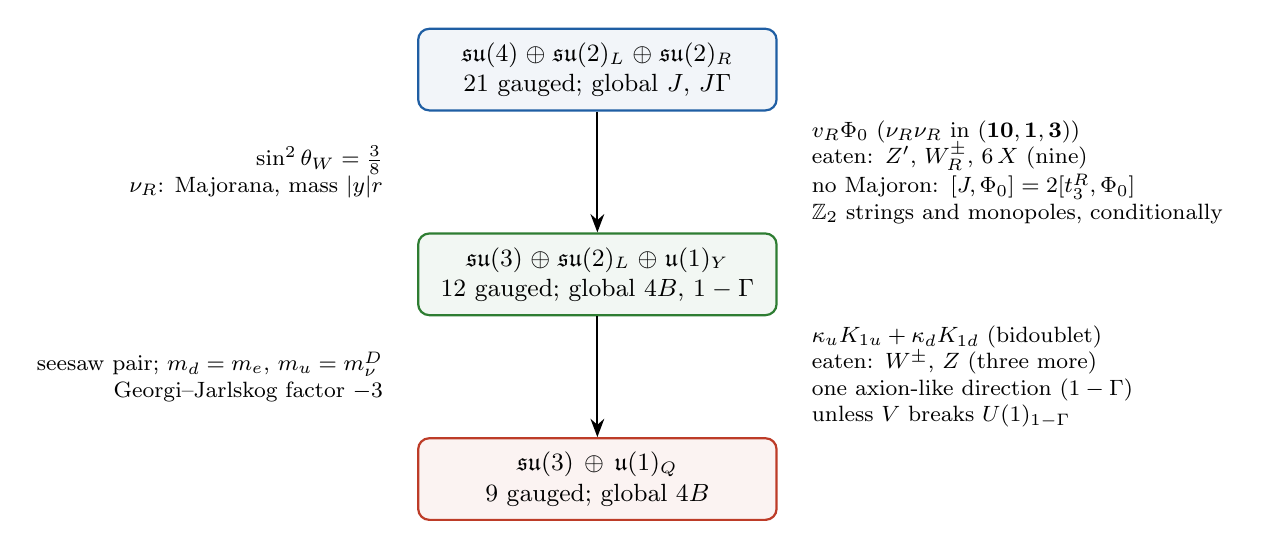
\begin{tikzpicture}[>=Stealth,font=\small,
  stage/.style={draw,thick,rounded corners=4pt,align=center,inner sep=5pt,text width=4.2cm},
  stp/.style={align=left,text width=5.3cm,font=\footnotesize},
  stpl/.style={align=right,font=\footnotesize}]
\node[stage,draw=tcol,fill=tcol!6] (ps) at (0,0) {$\su4\oplus\su2_L\oplus\su2_R$\\ $21$ gauged; global $J$, $J\Gamma$};
\node[stage,draw=gcol,fill=gcol!6] (sm) at (0,-2.6) {$\su3\oplus\su2_L\oplus\uu1_Y$\\ $12$ gauged; global $4B$, $1-\Gamma$};
\node[stage,draw=scol,fill=scol!6] (em) at (0,-5.2) {$\su3\oplus\uu1_Q$\\ $9$ gauged; global $4B$};
\draw[->,thick] (ps) -- (sm); \draw[->,thick] (sm) -- (em);
\node[stp,anchor=west] at (2.6,-1.3) {$v_R\Phi_0$ ($\nu_R\nu_R$ in $(\mathbf{10},\mathbf1,\mathbf3)$)\\ eaten: $Z'$, $W_R^\pm$, $6\,X$ (nine)\\ no Majoron: $[J,\Phi_0]=2[t^R_3,\Phi_0]$\\ $\Z_2$ strings and monopoles, conditionally};
\node[stp,anchor=west] at (2.6,-3.9) {$\kappa_uK_{1u}+\kappa_dK_{1d}$ (bidoublet)\\ eaten: $W^\pm$, $Z$ (three more)\\ one axion-like direction ($1-\Gamma$)\\ unless $V$ breaks $U(1)_{1-\Gamma}$};
\node[stpl,anchor=east] at (-2.6,-1.3) {$\sin^2\theta_W=\tfrac38$\\ $\nu_R$: Majorana, mass $|y|r$};
\node[stpl,anchor=east] at (-2.6,-3.9) {seesaw pair; $m_d=m_e$, $m_u=m_\nu^D$\\ Georgi--Jarlskog factor $-3$};
\end{tikzpicture}
\caption{The two stages of symmetry breaking in the selected vacuum (\cref{sec:matter,sec:goldstone}). Each arrow lists the order parameter, the vectors that
eat the Goldstone directions, and the uneaten directions attached to the global central charges.}
\label{fig:breaking}
\end{figure}

\subsection{Particles and antiparticles}

At one constituent charge conjugation is unique up to a $U(1)_J$ rotation, lies in the surplus plane and is the Majorana real structure (\cref{thm:C}), and the
Fock space of one momentum has a unique charge-zero ground state of energy $-2E$ (\cref{thm:spectra}). That value is the zero-point energy of two particle and two
antiparticle modes; summed over momenta it is the fermion term $-2\sum_{\rm Weyl}$ of the one-loop potential \eqref{eq:V1}, the very term through which matter
opposes the Standard-Model vacuum. At three constituents the discrete operations are classified as follows. A map $\psi\mapsto S\psi$ with $S$ orthogonal on $V_*$
exchanges particles and antiparticles when $SJ=-JS$; it keeps or reverses chirality according to $S\Gamma S^{-1}=\pm\Gamma$; it goes with $\mathbf x\mapsto-\mathbf x$ when
$S^{\!\top}K^iS=-K^i$.

\begin{theorem}[Four classes of discrete operators]
\label{thm:fourclasses}
The blades of $\Cl(9,9)$ that commute with the three involutions of $P_*$ and with the rotations number $8192$, and they fall into exactly four classes of $2048$:
internal ($J$-linear, $\Gamma$ kept, boosts kept), $P$ ($J$-linear, $\Gamma$ reversed, boosts reversed), $C$ ($J$-antilinear, $\Gamma$ reversed, boosts kept) and $CP$
($J$-antilinear, $\Gamma$ kept, boosts reversed). The two missing types are forbidden for every operator, since an antilinear map commuting with the Lorentz action and
keeping $\Gamma$ would identify $(\tfrac12,0)$ with its conjugate $(0,\tfrac12)$. Representatives are
\[
C=E_2E_7E_{10}E_{11}E_{12},\qquad P=O=E_1E_7E_8,\qquad CP=E_1E_2E_7E_8E_{10}E_{11}E_{12}E_{14},
\]
and all three normalise the Pati--Salam algebra and preserve the kinetic, gauge and Yukawa terms.
\end{theorem}

The factors of $C$ are instructive: $E_2$ is the surplus generator of the first constituent, where the one-constituent charge conjugation lives; $E_7$
exchanges left and right; and $E_{10}E_{11}E_{12}$, an odd number of colour generators, induces the outer automorphism of $\su4$ that exchanges $\mathbf4$ and
$\bar{\mathbf4}$. $P=O$ is parity composed with an $SU(2)$ Weyl reflection, and $CP=\pm(C\,O)\,E_7E_{14}$ with $E_7E_{14}$ a gauge element.

\begin{theorem}[$CP$ fixes the order parameter; $C$ and $P$ move it]
\label{thm:vacCP}
$CP\,\Phi_0\,CP^{\!\top}=\Phi_0$. $C\Phi_0C^{\!\top}$ is the $\nu_L\nu_L$ kernel, which commutes with $\su3$, $\su2_R$ and $Q$ but not with $\su2_L$, and
$P\Phi_0P^{\!\top}$ is the $e_Le_L$ kernel. Both images lie on the mirror orbit in $(\mathbf{10},\mathbf3,\mathbf1)$: the degeneracy of \cref{prop:LR} is realised by two distinct
discrete symmetries.
\end{theorem}

Invariance of the order parameter is not invariance of the theory. The kinetic, gauge and Yukawa terms and the trace invariants are $CP$-invariant; the general
potential on $\Kc$ is invariant only for couplings satisfying reality conditions; and on $(\mathbf{10},\mathbf1,\mathbf3)$ the holomorphic quartic needs a generalised $CP$,
composed with a baryon-number rotation $e^{\theta(J+H/3)}$, which is a classical symmetry of the renormalisable theory for every $\kappa$ but is anomalous, since $4B$
has $SU(2)_L^2$ anomaly $2$. Whether a $CP$ survives in the quantum theory is not settled.

Which fermions are their own antiparticles follows from a pairing rule. If $M$ is a mass kernel and $t$ an unbroken generator with $[t,M]=0$, then a Majorana-type $M$
satisfies $M\hat t=-\hat tM$, so within one chirality it pairs a representation of the unbroken group with its conjugate, while a Dirac-type $M$ pairs equal
representations of opposite chirality. A single irreducible multiplet can therefore carry a Majorana mass only if its representation of the unbroken group is
real: a nonzero charge under an unbroken $U(1)$ excludes this, while a nontrivial real representation of a non-abelian group does not. In the block, every multiplet
other than $\nu_R$ carries a nonzero hypercharge at the Pati--Salam stage, and every multiplet other than $\nu_L$ and $\nu_R$ is a colour triplet or electrically
charged at the electroweak stage. So $\nu_R$ is the only Majorana fermion at the first stage, the light $\nu$ and heavy $N$ of \cref{ex:EWspectrum} are the
Majorana fermions at the second, and the massive $\nu_R$ is mapped to itself by $CP$ with eigenvalues $\pm i$, since $CP^2=-\id$ on the block.

\subsection{Baryon number in the potential}

For a Pati--Salam invariant $\BmL=0$, so $4B=F$ and $\Delta B=F/4$ in terms of the fermion number $F$.

\begin{theorem}[Invariant polynomials by fermion number]
\label{thm:Bcounts}
The Pati--Salam-invariant polynomials on $\Kc$ of degrees two and four, graded by $F$, number
\begin{center}
\small
\begin{tabular}{@{}lcccc@{}}
\toprule
degree & $F=0$ & $F=\pm4$ ($|\Delta B|=1$) & $F=\pm8$ ($|\Delta B|=2$) & total\\
\midrule
$2$ & $12$ & $3+3$, all on $2(\mathbf6,\mathbf1,\mathbf1)$ & --- & $18$\\
$4$ & $402$ & $127+127$ & $15+15$, including $\mathcal D$ & $686$\\
\bottomrule
\end{tabular}
\end{center}
With $U(1)_F$ imposed the couplings number $12+402$; with $U(1)_{1-\Gamma}$, $8+228$; with both $F$ and $J\Gamma$-charge, $6+162$.
\end{theorem}

Pati--Salam gauge invariance alone does not forbid baryon-number violation. The six $F=\pm4$ quadratic invariants are holomorphic bilinears in the complex sextets
of $2(\mathbf6,\mathbf1,\mathbf1)$; under $\su3\oplus\uu1_{\BmL}$ each sextet is $\bar{\mathbf3}_{2/3}\oplus\mathbf3_{-2/3}$, diquark components coupling to quark pairs and leptoquark
components coupling to quark--lepton pairs, and $\epsilon^{abcd}\Delta_{ab}\Delta'_{cd}$ pairs one with the other. Through the Yukawa coupling such a mass mixing generates
tree-level $\Delta B=\Delta L=1$ four-fermion operators, of the type that mediates proton decay. Two protections are available and they are not equivalent: continuous
$U(1)_F$ forbids every $F\neq0$ term and conserves baryon number perturbatively (it is violated by $SU(2)$ instantons \cite{tHooft76}); the $\Z_4$ generated on $\Kc$ by
conjugation with $e^{\pi J/4}$ forbids the $|\Delta B|=1$ terms but allows the $|\Delta B|=2$ ones that mediate neutron--antineutron oscillation. $U(1)_F$, which the
radiative scenario of \cref{sec:selection} has, is sufficient, not necessary.

\subsection{Topology of the vacuum orbit}

\begin{theorem}[$\Z_2$ strings]
\label{thm:strings}
On the block $H=3J(\BmL)$, so $e^{\theta H}$ acts on quarks as $\cos\theta+J\sin\theta$ and on leptons as $\cos3\theta-J\sin3\theta$. The colour element $g_*=e^{\pi H/3}$ fixes
$\Phi_0$, acts as $-1$ on the $\nu_R$ line and on every lepton, and the path $\theta\mapsto e^{\theta H}\Phi_0e^{-\theta H}=\cos6\theta\,\Phi_0-\sin6\theta\,J\Phi_0$,
$\theta\in[0,\pi/3]$, is a closed loop on which the condensate phase winds once. Every generator of the stabiliser annihilates the $\nu_R$ line, so the identity component
of the stabiliser acts trivially there and $g_*$ is not in it. Lifting to $SU(4)\times SU(2)_L\times SU(2)_R$, the stabiliser has exactly two components, so the gauge orbit of
the vacuum has $\pi_1=\Z_2$, and $\pi_2\supseteq\Z$ from $U(1)_Y$.
\end{theorem}

If the gauge orbit is the complete set of minima of the chosen potential, as it is on $(\mathbf{10},\mathbf1,\mathbf3)$ in the region of \cref{thm:select0}, the vacuum supports
topologically stable $\Z_2$ strings around which $\nu_R$ changes sign, the Pati--Salam form of the $\Z_2$ strings of $\so{10}$ broken by a $\mathbf{126}$ \cite{KibbleLazaridesShafi82},
and Pati--Salam monopoles. If the minimum set is larger, as in the degenerate limit with accidental $O(272)$ symmetry, the relevant fundamental group is that of the
larger manifold, and a string may unwind through flat directions. The Standard-Model orbit and its mirror lie in different Pati--Salam components, so no gauge
transformation connects them; whether they are disconnected components of the full minimum set, which would give domain walls \cite{ZeldovichKobzarevOkun75},
depends on paths through configurations outside both orbits. Along the great circle of \cref{prop:LR} the radiative energy has a barrier between them for $x<27$,
but other paths are not controlled.

\part{Curvature, transport and the photon}
\section{A curved arena}
\label{sec:curved}

Nothing in the algebra requires the ambient metric to be flat. Promoting the metric to a field of signature $(3,3)$, the generators to an
orthonormal frame with a spin connection, and the pairing to a field of endomorphisms, one obtains a curved arena. This section describes its
geometry, builds one explicit curved model against which statements can be tested, and computes the six-dimensional Einstein tensor of that
model exactly. The two readings of $\R^{3,3}$ then each produce the Einstein tensor of a four-metric, in quite different ways, and neither
determines the metric.

\subsection{The pairing as a para-complex structure}

\begin{proposition}[The arena is almost para-Hermitian]
\label{prop:parahermitian}
Let $(M,g)$ have signature $(3,3)$ and let $\cK\in\End(TM)$ satisfy $\cK^2=\id$ and $g(\cK\cdot,\cK\cdot)=-g$. Then $(M,g,\cK)$ is almost
para-Hermitian: the eigendistributions $T^\pm M$ are isotropic of rank three, since $g(X,Y)=-g(\cK X,\cK Y)=-g(X,Y)$ on $T^+M$. It is
para-K\"ahler, equivalently bi-Lagrangian, if and only if $\nabla^{\rm LC}\cK=0$ for the Levi-Civita connection \cite{CruceanuFortunyGadea96,EtayoSantamaria06};
then each eigendistribution is parallel, involutive and totally geodesic, and $\Omega(X,Y)=g(\cK X,Y)$ is skew and closed.
\end{proposition}

The para-complex structure need not be posited: it is the grading root of \cref{prop:twoK}, $\cK(v)=\tfrac12[\mathsf P,v]$ with $\mathsf P=\sum_ie_ie_{i+3}$,
whose eigenspaces are the two totally null three-planes spanned by $e_i\mp e_{i+3}$. The null $3{+}3$ splitting it induces is a different
decomposition from the physical $4{+}2$ splitting into the interior four-plane and the surplus plane, and conflating them is the first thing to avoid. A
connection with torsion can preserve $\cK$ without making the eigendistributions integrable or $\Omega$ closed, so a $\cK$-preserving connection does not
deliver the para-K\"ahler conclusion \cite{MarottaSzabo21,LoustauSanders22}. Para-K\"ahler geometry is the world of $\cK^2=+\id$, while chirality is
comfortable in the world of $J^2=-\id$; this is one way of naming the difficulty that runs through the whole construction.

\subsection{An explicit model with a normal $U(1)$}
\label{sec:curvedmodel}

Split the tangent space as $TM=E\oplus N$ with $E=\operatorname{span}\{\widehat W,e_4,e_5,e_6\}$ of signature $(1,3)$, the symmetric clock of
\cref{prop:clock} playing the role of $\gamma^0$, and $N=\operatorname{span}\{u_1,u_2\}$ with
\[
u_1=\tfrac1{\sqrt2}(e_1-e_2),\qquad u_2=\tfrac1{\sqrt6}(e_1+e_2-2e_3),
\]
which complete the clock inside the positive triple: the relative times of \cref{sec:clocksimplex}. The metric does not select this split; it is extra
data.

\begin{lemma}[The normal plane carries a commuting rotation]
\label{lem:JN}
$J_N:=u_1u_2=\tfrac1{\sqrt3}(e_2e_3+e_3e_1+e_1e_2)$ satisfies $J_N^2=-\id$ and commutes with $\widehat W$, $e_4$, $e_5$ and $e_6$.
\end{lemma}

\begin{proof}
$J_N$ is a sum of time--time bivectors and has no spatial index, so it commutes with $e_4,e_5,e_6$ by \eqref{eq:bladecomm}; it is the unit bivector of
the plane orthogonal to $\widehat W$ inside the positive triple, so it commutes with $\widehat W$; and $u_1,u_2$ are orthonormal of square $+\id$, so
$(u_1u_2)^2=-u_1^2u_2^2=-\id$.
\end{proof}

The normal plane therefore carries a compact $\uu1$ commuting with the physical generators. Give it a connection, $\nabla^\perp u_1=-Au_2$,
$\nabla^\perp u_2=Au_1$, with spin connection $\Omega_N=\tfrac12AJ_N$. The model metric is
\begin{equation}
\label{eq:kk}
ds_6^2=g^{(4)}_{\mu\nu}(x)\,dx^\mu dx^\nu+(du+vA)^2+(dv-uA)^2,\qquad A=A_\mu(x)\,dx^\mu .
\end{equation}

\begin{proposition}[The model]
\label{prop:kk}
The metric \eqref{eq:kk} has signature $(3,3)$; its restriction to $\Sigma=\{u=v=0\}$ is $g^{(4)}$; the induced normal connection is $A$; and
$R^u{}_{v\mu\nu}|_\Sigma=(dA)_{\mu\nu}$. For $g^{(4)}$ flat and $A=Bx\,dz$ one finds $R^u{}_{vxz}|_\Sigma=B$ while every component $R^\mu{}_{\nu\rho\sigma}|_\Sigma$
vanishes.
\end{proposition}

This is the Kaluza--Klein construction for a rank-two real bundle with structure group $SO(2)$, and $R^u{}_{v\mu\nu}=F_{\mu\nu}$ is the standard formula for
the curvature of a normal bundle \cite{AppelquistChodosFreund87,ONeill83}. Two consequences are easy to misread in either direction: ambient curvature does
not imply observable curvature, since the last example has a curved six-geometry with a flat induced four-metric; and a four-dimensional distribution is not
a spacetime until an integral submanifold or a quotient is produced, which here $\Sigma$ supplies.

\begin{proposition}[The surplus constraints are first class]
\label{prop:constraints}
For a geodesic test particle in \eqref{eq:kk} put $\ell=vp_u-up_v$, $k_\mu=p_\mu-A_\mu\ell$, so that $H=\tfrac12(g_{(4)}^{\mu\nu}k_\mu k_\nu+p_u^2+p_v^2)$. With
$\phi_1=p_u$, $\phi_2=p_v$ and $C:=A_\mu g_{(4)}^{\mu\nu}k_\nu$,
\[
\{\phi_1,\phi_2\}=0,\qquad \{\phi_1,H\}=-C\phi_2,\qquad \{\phi_2,H\}=+C\phi_1 ,
\]
so the constraints are first class for every $A_\mu(x)$ and every $g^{(4)}$. The reduced phase space has dimension $12-2\times2=8$, that of $T^*M^4$, and
$H_{\rm red}=\tfrac12g_{(4)}^{\mu\nu}p_\mu p_\nu$.
\end{proposition}

The potential has cancelled from the reduced Hamiltonian, and not by accident: the constraints generate translations in $(u,v)$, so the normal $U(1)$
acts trivially on the reduced phase space and a spinless test particle cannot see it. Whatever makes the normal connection physical must come from the
spinor sector, which \cref{sec:transport} examines. This is a first instance of the constraint structure that \cref{sec:constraints} derives from a
worldline gauge symmetry.

\subsection{The six-dimensional Einstein tensor}
\label{sec:ambientEin}

In polar normal coordinates $u+iv=re^{i\phi}$ the model reads $ds_6^2=h_{\mu\nu}dx^\mu dx^\nu+dr^2+r^2(d\phi-A)^2$ with $h=g^{(4)}$. Write
$W_{\mu\nu}=F_{\mu\rho}F_\nu{}^\rho-\tfrac14h_{\mu\nu}F^2$. In signature $(+,-,-,-)$, $-W_{00}=\tfrac12(|\bE|^2+|\bB|^2)$, so a physical Maxwell field enters
Einstein's equation as $\mathcal G=-2W$ in units where the coupling is absorbed.

\begin{theorem}[The ambient Einstein tensor]
\label{thm:ein6}
For every $r>0$, and not as a series in $r$,
\[
\mathcal G^{(6)}_{\mu\nu}=\mathcal G_{\mu\nu}[h]-\tfrac{r^2}2W_{\mu\nu},\qquad \mathcal G^{(6)}_{rr}=-\tfrac12R[h]+\tfrac{r^2}8F^2,\qquad
\mathcal G^{(6)}_{\hat\phi\hat\phi}=-\tfrac12R[h]+\tfrac{3r^2}8F^2,
\]
\[
\mathcal G^{(6)}_{\mu\hat\phi}=\tfrac r2\nabla^\rho F_{\rho\mu},\qquad \mathcal G^{(6)}_{\mu r}=\mathcal G^{(6)}_{r\hat\phi}=0,\qquad R^{(6)}=R[h]-\tfrac{r^2}4F^2,
\]
with indices and $\nabla$ referring to $h$. On the slice $\Sigma$ the Einstein tensor is
\[
\mathcal G^{(6)}\big|_\Sigma=\operatorname{diag}\bigl(\mathcal G_{\mu\nu}[h],\,-\tfrac12R[h],\,-\tfrac12R[h]\bigr):
\]
its tangential block is the four-dimensional Einstein tensor exactly, with no stress term from $F$.
\end{theorem}

\begin{proof}
The projection onto $(M,h)$ is a semi-Riemannian submersion with flat, totally geodesic fibres: for $U,V\in\{\partial_r,\partial_\phi\}$ and the horizontal lifts
$E_\mu=\partial_\mu+A_\mu\partial_\phi$ one has $[U,E_\mu]=0$ and $E_\mu\,g(U,V)=0$, so the Koszul formula gives $g(\nabla_UV,E_\mu)=0$. The integrability tensor is
$\tfrac12[E_\mu,E_\nu]^{\rm vert}=\tfrac12F_{\mu\nu}\partial_\phi$ with $|\partial_\phi|^2=r^2$. O'Neill's formulas, valid for semi-Riemannian submersions with nondegenerate
fibres \cite{ONeill66,ONeill83,Besse87}, then give $R^{(6)}_{\mu\nu}=R_{\mu\nu}[h]-\tfrac{r^2}2F_{\mu\rho}F_\nu{}^\rho$, $R^{(6)}_{\mu\hat\phi}=\tfrac r2\nabla^\rho F_{\rho\mu}$,
$R^{(6)}_{\hat\phi\hat\phi}=\tfrac{r^2}4F^2$ and $R^{(6)}_{rr}=0$, from which the Einstein components follow. They have also been checked symbolically on a Friedmann base
$h=\operatorname{diag}(1,-t^2,-t^2,-t^2)$ with $A=z\,dt+\tfrac12x^2dy$, which carries both electric and magnetic fields.
\end{proof}

\begin{corollary}[Sign, reduction and rigidity]
\label{cor:ein6}
\begin{enumerate}[label=(\roman*),leftmargin=2.2em]
\item The tangential equation $\mathcal G[h]=+\tfrac{r^2}2W$ has the opposite sign to $\mathcal G=-2W$: the normal field strength gravitates with negative energy.
The sign is forced: a Lorentzian four-plane in $\R^{3,3}$ uses one positive and three negative directions, so its normal plane has signature $(2,0)$, the
sign of time.
\item Over a normal disc of radius $r_c$, $\int\!\!\int\sqrt{|g_6|}\,R^{(6)}\,d\phi\,dr=\sqrt{|h|}\bigl(\pi r_c^2R[h]-\tfrac{\pi r_c^4}8F^2\bigr)$. The Euler--Lagrange
equation of $\int\sqrt{|h|}(a_1R+a_2F^2)$ is $a_1\mathcal G+2a_2W=0$, so Einstein--Maxwell theory has $a_2/a_1=+1$ while the reduced action has $a_2/a_1=-r_c^2/8$: the
wrong relative sign.
\item The vacuum is rigid: $\mathcal G^{(6)}=0$ if and only if $F=0$ and $h$ is Ricci-flat. The internal equations differ by $\tfrac{r^2}4F^2$, which forces $F^2=0$ and
then $R[h]=0$; the tangential equation must hold at every $r$ while $\mathcal G[h]$ and $W$ do not depend on $r$, so $\mathcal G[h]=0$ and $W=0$ separately, and $W=0$
forces $F=0$ because $-W_{00}$ is positive definite.
\end{enumerate}
\end{corollary}

Reduction on directions of timelike sign is known to give fields whose kinetic terms have the wrong sign \cite{Hull98}, and the negative-energy vector
found here is an instance. The two mechanisms of rigidity can be separated by changing the fibre. With a normal fibre of constant size,
$ds_6^2=h+\ell^2(d\psi-A)^2+m^2d\chi^2$, still of signature $(3,3)$, the internal equations force only $F^2=0$, and null fields survive.

\begin{example}[Negative-energy null radiation]
\label{ex:nullwave}
Take $h=2\,dU\,dV-H\,dU^2-dX^2-dY^2$ and $A=a(U)X\,dU$, so $F=a(U)\,dX\wedge dU$ is null. The only nonzero component of the six-dimensional Einstein tensor is
$\mathcal G^{(6)}_{UU}=-\tfrac12(H_{XX}+H_{YY}-\ell^2a^2)$, so
\[
H=\tfrac14\ell^2a(U)^2(X^2+Y^2)
\]
solves the six-dimensional vacuum with $F\neq0$. In four-dimensional terms $\mathcal G_{UU}[h]=-\tfrac12\ell^2a^2<0$, whereas a physical null Maxwell wave has
$\mathcal G_{UU}=-2W_{UU}=+2a^2>0$: the wave is negative-energy radiation. With the fibre size the coordinate $r$, as in \eqref{eq:kk}, the same field gives a
tangential component graded in $r$ that forces $a=0$.
\end{example}

More generally, with $ds_6^2=h+e^{2\alpha(x)}(d\psi-A)^2+e^{2\beta(x)}d\chi^2$,
\[
\mathcal G^{(6)}_{\hat\psi\hat\psi}-\mathcal G^{(6)}_{\hat\chi\hat\chi}=\tfrac14e^{2\alpha}F^2-\Box(\alpha-\beta)-\nabla(\alpha-\beta)\cdot\nabla(\alpha+\beta).
\]
For a breathing mode $\alpha=\beta$ the difference is a pure constraint and only null $F$ survives; for a relative modulus it is a field equation for $\alpha-\beta$,
and $F^2\neq0$ becomes admissible. Non-null $F$ therefore needs the ratio of the two normal sizes to be a dynamical field. None of these escapes repairs
the sign.

\subsection{Off the slice}

On $\Sigma$ the $F$-couplings, which all carry $r$, switch off. Taking the four-geometry off the zero section requires care, because the level set
$\{r=r_0\}$ is five-dimensional. Its quotient by the $U(1)$ is four-dimensional and carries $h$, and the ambient Einstein tensor in the horizontal frame is
$\mathcal G[h]-\tfrac{r_0^2}2W$, with the sign above. A section $\phi=\chi(x)$ of $\{r=r_0\}$ is a four-dimensional submanifold with induced metric
\[
h_\chi=h+r_0^2\,B\otimes B,\qquad B:=d\chi-A ,
\]
where $B$ is the St\"uckelberg combination, invariant under $A\mapsto A+d\lambda$, $\chi\mapsto\chi+\lambda$; $\det h_\chi=\det h\,(1+r_0^2|B|^2)$, so $h_\chi$ is Lorentzian
only where $1+r_0^2|B|^2>0$, and the section is totally geodesic on an open set only where $B=0$, which requires $F=0$.

\begin{example}[A uniform magnetic field]
\label{ex:landau}
Take $h=\eta$ and $F=b\,dx\wedge dz$. On a static section the circulation of $B$ around a circle of radius $R_c$ in an $x$--$z$ plane is $-\pi bR_c^2$, whatever $\chi$,
so $\sum_iB_i^2\ge b^2R_c^2/4$ somewhere on it, and the section metric has signature $(2,2)$ there as soon as $R_c>2/(r_0b)$. In the gauge $A=bx\,dz$ with $\chi=0$,
\[
h_\chi=dt^2-dx^2-dy^2-(1-k^2x^2)\,dz^2,\qquad R[h_\chi]=-\frac{2k^2}{(1-k^2x^2)^2},\qquad k=r_0b,
\]
which degenerates at $|x|=1/k$, where its curvature diverges, and has signature $(2,2)$ beyond. The Lorentzian region of a static section in a uniform field
contains no circle of radius larger than $2/(r_0b)$.
\end{example}

\subsection{Holonomy acting on the bound orbits}

The interior dynamics of \cref{sec:neutral} can now be transported around a loop of the model. A circuit enclosing normal flux $\Phi$ rotates the frame by
$h=\exp(\Phi R_N)$, with $R_N$ the rotation of the normal plane $N$. $R_N$ preserves $\eta$, but it rotates a temporal plane without its spatial partner, so it is not
among the diagonal rotations of \cref{thm:GLorentz}, and exactly
\[
h=\id+\sin\Phi\,R_N+(1-\cos\Phi)R_N^2,\qquad hGh^{-1}-G=\sin\Phi\,A_1+(1-\cos\Phi)\,A_2
\]
with $A_1,A_2$ linearly independent, so $hGh^{-1}=G$ if and only if $\Phi\in2\pi\Z$. The second-order equation $\ddot X=-\kappa^2X$ does not see this, but the momentum
does: a zero-momentum orbit $X(\tau)=e^{-\kappa G\tau}X_0$ carried once around becomes $hX(\tau)$, and
\[
\alpha_+(hX)=\kappa\,(G-hGh^{-1})\,hX ,
\]
which vanishes for every $X_0$ only when $\Phi\in2\pi\Z$. Normal curvature therefore converts bound orbits of zero momentum into orbits that carry momentum, through
exactly the failure of the normal $U(1)$ to centralise the binding root.

\subsection{Flows do not transfer}

In DeTurck gauge Ricci flow reads $\partial_tg_{MN}=\Delta_gg_{MN}+Q(g,\partial g)$, and short-time existence requires the principal symbol $g^{PQ}\xi_P\xi_Q$ to be
definite \cite{Hamilton82,DeTurck83}. In signature $(3,3)$ it has signature $(3,3)$: the operator is ultrahyperbolic, the gauge-fixed flow is not parabolic, and the
standard Ricci--DeTurck theory does not apply. In the para-K\"ahler case the metric comes locally from a potential depending on coordinates along both
foliations, $g_{i\bar\jmath}=\partial^2\Phi/\partial x^i\partial y^j$ \cite{Shima07}, but suppressing one set of variables degenerates the metric rather than producing a Hessian
one; a real Monge--Amp\`ere flow on a convex locus \cite{Cao85} would need its own domain, data and a proof that it preserves the arena's structures, and is a
programme rather than a result.

\section{Curvature in the field-strength reading}
\label{sec:curvop}

In the field-strength reading the six directions are $\Lambda^2\R^{1,3}$, $\eta$ is the induced metric and $G$ the Hodge star (\cref{thm:emfield}). A
tensor $R_{abcd}$ antisymmetric in each pair is then an operator $\cR$ on the frame, $(\cR\omega)_{ab}=\tfrac12R_{ab}{}^{cd}\omega_{cd}$ \cite{SingerThorpe69,Besse87},
and the conditions that make it a Riemann tensor become conditions stated with $\eta$ and $G$. Write $\Ric(\cR)_{bd}=R^a{}_{bad}$.

\begin{proposition}[The curvature operator lives on the frame]
\label{prop:curvop}
$\cR$ comes from a pair-symmetric tensor, $R_{abcd}=R_{cdab}$, if and only if $\cR$ is $\eta$-self-adjoint, a $21$-dimensional space $\mathcal S$; the
$\eta$-antisymmetric operators give $R_{abcd}=-R_{cdab}$ instead. On $\mathcal S$, $\Tr\cR=\tfrac12R$ and
\[
R_{abcd}+R_{acdb}+R_{adbc}=-\tfrac12\Tr(G\cR)\,\varepsilon_{abcd},\qquad \varepsilon_{0123}=+1,
\]
so the first Bianchi identity is the single linear condition $\Tr(G\cR)=0$, and the algebraic curvature operators form a $20$-dimensional subspace $\mathcal V$,
the dimension of the space of Riemann tensors in four dimensions.
\end{proposition}

Pair symmetry is the same condition $G=G^\dagger$ that makes the interior shift factorise (\cref{thm:neutral}), imposed on an operator of another type: the frame
is shared, not the object. The binding root, which is $\eta$-self-adjoint, is itself in $\mathcal S$ but not in $\mathcal V$, since $\Tr(G\cdot G)=-6$; it is the one
direction of $\mathcal S$ that violates the Bianchi identity.

\subsection{A phase family that ends at the Einstein tensor}

\begin{theorem}[The phase family]
\label{thm:phase}
For every $\cR\in\mathcal S$, on or off the Bianchi shell, and every $\theta$, the operator $\cR_\theta:=e^{\theta G}\cR\,e^{\theta G}$ lies in $\mathcal S$ and
\[
\Ric(\cR_\theta)_{ab}=R_{ab}-\tfrac12\sin^2\theta\,R\,g_{ab}+\tfrac12\sin2\theta\,\Tr(G\cR)\,g_{ab}.
\]
At $\theta=\pi/2$ the operator is the double dual $G\cR G$ of Lanczos \cite{Lanczos38,MTW}, and its contraction is the Einstein tensor $R_{ab}-\tfrac12Rg_{ab}$.
\end{theorem}

\begin{proof}
Two lemmas hold on all of $\mathcal S$: $\Ric(G\cR G)=\Ric(\cR)-\tfrac12Rg$, and $\Ric(G\cR)+\Ric(\cR G)=\Tr(G\cR)\,g$. With $e^{\theta G}=\cos\theta+\sin\theta\,G$,
\[
\cR_\theta=\cos^2\theta\,\cR+\sin\theta\cos\theta\,(G\cR+\cR G)+\sin^2\theta\,G\cR G ,
\]
and the lemmas contract this to the formula. It has also been checked as a polynomial identity in the $21$ entries, modulo $\cos^2\theta+\sin^2\theta=1$. Since $G$ is
$\eta$-self-adjoint, so is $e^{\theta G}$, and $\cR_\theta\in\mathcal S$.
\end{proof}

\begin{example}[A maximally symmetric curvature]
\label{ex:dS}
For de Sitter space of curvature $k$, $R_{abcd}=k(g_{ac}g_{bd}-g_{ad}g_{bc})$, the curvature operator is $\cR=k\,\id$ on the frame up to the sign convention of the
induced metric, so $\Tr\cR=6k=\tfrac12R$ gives $R=12k$ and $\Tr(G\cR)=k\Tr G=0$. Then $G\cR G=kG^2=-k\,\id$, and the formula gives
$\Ric(\cR_{\pi/2})=R_{ab}-\tfrac12Rg_{ab}=3kg_{ab}-6kg_{ab}=-3kg_{ab}$, the Einstein tensor of de Sitter space, which is $-\Lambda g_{ab}$ with $\Lambda=3k$. The double
dual of a constant-curvature operator is minus itself, and the trace reversal that turns Ricci into Einstein is the sign change $G^2=-\id$.
\end{example}

\begin{corollary}[What selects the endpoint]
\label{cor:phasesel}
\begin{enumerate}[label=(\roman*),leftmargin=2.2em]
\item For the curvature operator of a metric and a constant phase, the contracted Bianchi identity gives $\nabla^aH_{ab}(\theta)=\tfrac12\cos^2\theta\,\nabla_bR$ for
$H(\theta):=\Ric(\cR_\theta)$, so divergence-freedom for every metric selects $\theta\equiv\pi/2\pmod\pi$.
\item $\Tr(G\cR_\theta)=\cos2\theta\,\Tr(G\cR)-\tfrac12\sin2\theta\,R$, so on the Bianchi shell and for $R\neq0$, $\cR_\theta$ is itself a curvature operator only at
$\sin2\theta=0$, compatible with (i) and narrowing nothing further.
\item $Q(\cR):=\tfrac12\Tr(\cR G\cR G)=-\tfrac18\bigl(R^2-4R_{ab}R^{ab}+R_{abcd}R^{abcd}\bigr)$ for every pair-symmetric $\cR$, and $dQ[\mathcal D]=\Tr(G\cR G\mathcal D)$: the
double dual is the algebraic gradient of the Gauss--Bonnet density, exactly so on $\mathcal V$, where $G\cR G=\operatorname{grad}_{\mathcal V}Q$.
\end{enumerate}
\end{corollary}

The gradient in (iii) does not lift to a field equation. The spacetime integral of the Gauss--Bonnet density has identically vanishing metric variation in four
dimensions, which is Lanczos's identity \cite{Lanczos38,Lovelock71}: the Euler--Lagrange tensor $P_a{}^{cde}R_{bcde}-\tfrac12g_{ab}\mathcal E_{\rm GB}-2\nabla^c\nabla^dP_{acdb}$ with
$P=-2\,{*R*}$ vanishes because the double dual is divergence-free and $(*R*)_a{}^{cde}R_{bcde}=-\tfrac14g_{ab}\mathcal E_{\rm GB}$ in four dimensions. The two facts sit one
Lovelock degree apart: the algebraic gradient of the quadratic density contracts to the metric gradient of the linear density $\Tr\cR=\tfrac12R$, and the quadratic
density itself is inert. Which members of the family are variational at all is a sharper question, and it has a sharp answer.

\begin{theorem}[Only the Einstein phase is variational]
\label{thm:helmholtz}
Consider the operators $g\mapsto H(\theta)[g]_{ab}=R_{ab}-\tfrac12\sin^2\theta\,Rg_{ab}$. There is a Lagrangian $L(g,\partial g,\partial^2g,\dots)$, covariant or not, defined
on a neighbourhood of flat space, whose Euler--Lagrange expression is $H(\theta)$ if and only if $\cos\theta=0$; then $R\sqrt{|g|}$ is one.
\end{theorem}

\begin{proof}
An Euler--Lagrange operator has a formally self-adjoint Fr\'echet derivative at every point of its domain, the necessity half of the Helmholtz conditions
\cite{Vainberg64,Olver93}. At $g=\eta$, $H(\theta)[\eta]=0$, so the density factor does not contribute and the linearisation acts on plane waves $h_{ab}e^{ik\cdot x}$ with a
symbol quadratic in $k$. Pairing it with a second perturbation $q_{ab}$, the antisymmetric part of the bilinear form is
\[
q^{ab}\,\delta H_{ab}[h]-h^{ab}\,\delta H_{ab}[q]=\tfrac12\cos^2\theta\bigl[(k\cdot q\cdot k)\,\tr h-(k\cdot h\cdot k)\,\tr q\bigr],
\]
which vanishes identically only when $\cos\theta=0$. There the operator is the Einstein tensor, and $\delta(R\sqrt{|g|})=\sqrt{|g|}\,\mathcal G_{ab}\,\delta g^{ab}$ up to a
divergence.
\end{proof}

For a diffeomorphism-invariant action Noether's second theorem makes the Euler--Lagrange tensor divergence-free, so \cref{cor:phasesel}(i) is the covariant
necessary condition and \cref{thm:helmholtz} the full condition, obtained without assuming covariance. Both select the same phase.

\subsection{The first-order form: the phase is a Barbero--Immirzi angle}

Let $e^a$ be a coframe, $\omega$ a Lorentz connection with curvature $F^{ab}$, and $\Sigma^{ab}=e^a\wedge e^b$. Both $\Sigma$ and $F$ are two-forms valued in
$\Lambda^2\R^{1,3}$, which is the frame by \cref{thm:emfield}. Pair them by $\langle\Sigma\wedge X\rangle=\tfrac12\Sigma_{ab}\wedge X^{ab}$, orient by
$\mathrm{vol}=e^0\wedge e^1\wedge e^2\wedge e^3$, and let $\cR$ be the curvature operator of $\omega$ in the frame $e$.

\begin{proposition}[Palatini and Holst on the frame]
\label{prop:holst}
\begin{enumerate}[label=(\roman*),leftmargin=2.2em]
\item $\tfrac14\varepsilon_{abcd}\,e^a\wedge e^b\wedge F^{cd}=\langle G\Sigma\wedge F\rangle=\Tr(\cR)\,\mathrm{vol}$: the Palatini Lagrangian, which on the torsion-free
locus is $\tfrac12R\,\mathrm{vol}$.
\item $e_a\wedge e_b\wedge F^{ab}=2\langle\Sigma\wedge F\rangle=-2\Tr(G\cR)\,\mathrm{vol}$: the Holst term is the first-Bianchi datum of \cref{prop:curvop}.
\item For the phase family, $\langle e^{\theta G}\Sigma\wedge e^{\theta G}F\rangle=\cos2\theta\,\langle\Sigma\wedge F\rangle+\sin2\theta\,\langle G\Sigma\wedge F\rangle=-\Tr(G\cR_\theta)\,\mathrm{vol}$.
In the normalisation $\tfrac12\varepsilon_{abcd}e^ae^bF^{cd}-\gamma^{-1}e_ae_bF^{ab}$ this is the Holst action \cite{Holst96} with
\[
\gamma=-\tan2\theta ,
\]
the Barbero--Immirzi parameter.
\item The connection equation of $\int\langle e^{\theta G}\Sigma\wedge e^{\theta G}F\rangle$ is $e^{2\theta G}D\Sigma=0$, so the torsion vanishes, and the coframe equation is
$-2\sin2\theta\,\mathcal G^{af}=0$ on the torsion-free locus. The vacuum equations are Einstein's for every $\theta\notin\tfrac\pi2\Z$ and empty for $\theta\in\tfrac\pi2\Z$.
\end{enumerate}
\end{proposition}

\begin{figure}[t]
\centering
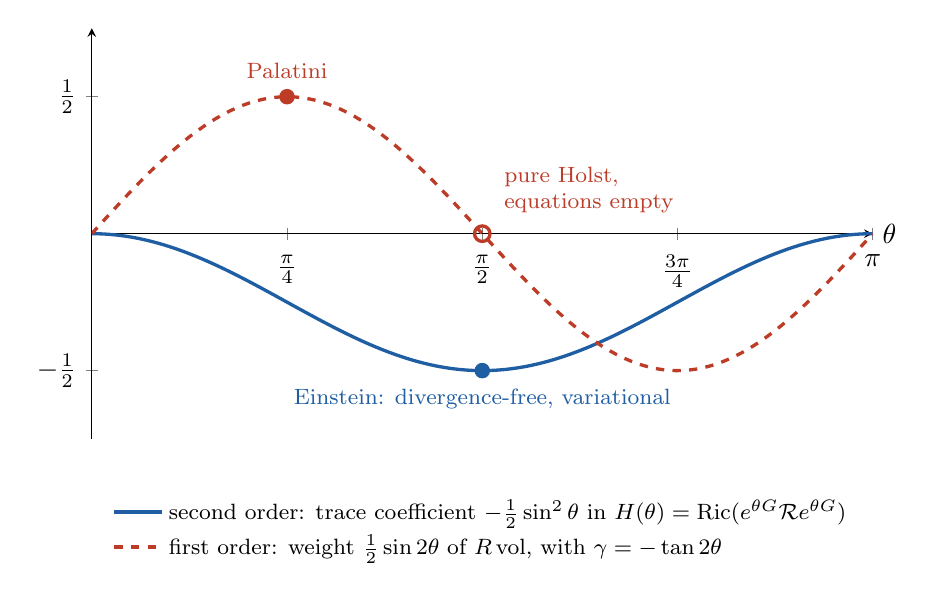
\begin{tikzpicture}
\begin{axis}[width=11.5cm,height=6.8cm,xmin=0,xmax=3.1416,ymin=-0.75,ymax=0.75,axis lines=middle,
  xtick={0,0.7854,1.5708,2.3562,3.1416},xticklabels={$0$,$\frac\pi4$,$\frac\pi2$,$\frac{3\pi}4$,$\pi$},
  ytick={-0.5,0.5},yticklabels={$-\frac12$,$\frac12$},xlabel={$\theta$},
  xlabel style={anchor=west},x tick label style={yshift=-2pt},
  legend style={at={(0.5,-0.12)},anchor=north,font=\footnotesize,draw=none,legend columns=1},legend cell align=left]
\addplot[tcol,very thick,domain=0:3.1416,samples=120] {-0.5*sin(deg(x))^2};
\addlegendentry{second order: trace coefficient $-\frac12\sin^2\theta$ in $H(\theta)=\Ric(e^{\theta G}\cR e^{\theta G})$}
\addplot[scol,very thick,dashed,domain=0:3.1416,samples=120] {0.5*sin(deg(2*x))};
\addlegendentry{first order: weight $\frac12\sin2\theta$ of $R\,\mathrm{vol}$, with $\gamma=-\tan2\theta$}
\addplot[only marks,mark=*,mark size=2.6pt,tcol,forget plot] coordinates {(1.5708,-0.5)};
\addplot[only marks,mark=*,mark size=2.6pt,scol,forget plot] coordinates {(0.7854,0.5)};
\addplot[only marks,mark=o,mark size=2.8pt,scol,very thick,forget plot] coordinates {(1.5708,0)};
\node[tcol,anchor=north,font=\footnotesize,align=center] at (axis cs:1.5708,-0.53) {Einstein: divergence-free, variational};
\node[scol,anchor=south,font=\footnotesize] at (axis cs:0.7854,0.53) {Palatini};
\node[scol,anchor=south west,font=\footnotesize,align=left] at (axis cs:1.62,0.04) {pure Holst,\\ equations empty};
\end{axis}
\end{tikzpicture}
\caption{Two uses of one duality rotation of the curvature (\cref{thm:phase,thm:helmholtz,prop:holst}). In the second-order family $H(\theta)=\Ric(e^{\theta G}\cR e^{\theta G})$
the endpoint $\theta=\pi/2$ is the Einstein tensor, the only divergence-free and the only variational member. In the first-order family the same rotation weights the
Einstein--Hilbert term by $\tfrac12\sin2\theta$: Einstein's equations follow for every $\theta\notin\tfrac\pi2\Z$, the Palatini point is $\pi/4$, and at $\theta=\pi/2$ the Lagrangian
degenerates to the pure Holst term, with $\gamma=-\tan2\theta$.}
\label{fig:phase}
\end{figure}

The roles of the phase differ between the two formalisms, as \cref{fig:phase} shows. In the second-order family the variational point is $\theta=\pi/2$; in the
first-order family Einstein's equations hold for every $\theta\notin\tfrac\pi2\Z$, the Palatini point is $\theta=\pi/4$, and the endpoint $\theta=\pi/2$, where $\cR_\theta=G\cR G$, is
exactly where the first-order Lagrangian degenerates to the pure Holst term. These are two uses of one rotation and must not be conflated. The self-dual value
$\gamma=\pm i$ of Ashtekar's variables is not attained for any complex $\theta$; it is approached as $\Im\theta\to\mp\infty$, where $e^{2\theta G}$ becomes proportional to a
projector onto an eigenspace of $G$. With torsion sources such as fermions the Holst term is no longer inert and the phase would enter an effective four-fermion
interaction \cite{PerezRovelli06,FreidelMinicTakeuchi05}; nothing here fixes it.

Both readings of $\R^{3,3}$ therefore construct the Einstein tensor of a given four-metric: the interior reading by restricting the six-dimensional Einstein tensor to
the slice (\cref{thm:ein6}), the field-strength reading as the contraction of $G\cR G$ (\cref{thm:phase}). Neither determines the metric. No gravitational coupling,
source or equation of motion for $G$ follows, the selection criteria come from Riemannian geometry rather than from the Clifford structure, and the coefficient
$\tfrac12$ of the trace reversal comes from the algebra of the Hodge star.

\section{The projector under transport}
\label{sec:transport}

In a curved arena an observation projector becomes a field $\Pi(x)=\Pi(x)^2$ that is carried around by the spin connection, $D\Pi=d\Pi+[\Omega,\Pi]$. Two
curvatures then compete on its image, and their competition decides whether the normal $U(1)$ of the model of \cref{sec:curvedmodel} can be electromagnetism.

\subsection{Two curvatures on the selected bundle}

Differentiating $\Pi^2=\Pi$ gives $\Pi(D\Pi)\Pi=0$ and $(\id-\Pi)(D\Pi)(\id-\Pi)=0$: the covariant derivative of a projector is purely off-diagonal, which is the
configuration-space statement of \cref{sec:fields} in covariant form. The induced connection $D^{\rm obs}s=\Pi Ds$ on the selected bundle has curvature
\begin{equation}
\label{eq:Fobs}
\mathcal F_{\rm obs}=\Pi\,\mathcal R\,\Pi+\Pi\,(D\Pi\wedge D\Pi)\,\Pi ,
\end{equation}
with $\mathcal R_{MN}=\tfrac14R_{MNAB}\gamma^A\gamma^B$ the ambient spin curvature \cite{LawsonMichelsohn}. The two terms have distinct origins: ambient curvature, and the
motion of the selected subspace relative to ambient transport. The flat case of \cref{sec:fields} keeps only the second.

\begin{proposition}[Transport obstruction]
\label{prop:obstruct}
If ambient transport preserves the projector, $D\Pi=0$, then $[\mathcal R_{MN},\Pi]=0$. For the paired-mode projector $\Pi=\tfrac12\id-\tfrac14(\mathsf P+\mathcal V)$ of
\cref{ex:pairedmode}, $\rank[J_N,\Pi]=4$, and in the model \eqref{eq:kk} with $g^{(4)}$ flat, $\mathcal R_{\mu\nu}=\tfrac12(F_N)_{\mu\nu}J_N$ on $\Sigma$, so
$[\mathcal R_{\mu\nu},\Pi]=\tfrac12(F_N)_{\mu\nu}[J_N,\Pi]\neq0$ wherever the normal curvature $F_N=dA$ is nonzero.
\end{proposition}

\begin{proof}
$D^2\Pi=[\mathcal R,\Pi]$ for any section of the endomorphism bundle, so $D\Pi=0$ forces the condition. The rank is a direct computation in the $8\times8$ realisation.
\end{proof}

This statement is about the spinor projector and the spin curvature, and the corresponding tangent-level statement is false; the two must not be run together.
At the tangent level $J_N$ commutes with every generator of $E$ (\cref{lem:JN}), so the rotation it generates fixes $E$ pointwise, and in \eqref{eq:kk} every
mixed Christoffel symbol vanishes on $\Sigma$: the splitting $TM=E\oplus N$ is Levi-Civita parallel there although $F_N\neq0$. At the spinor level the same rotation is
not trivial, since $\rank[J_N,\Pi]=4$. Both statements hold simultaneously, and together they are the content of the remark after \cref{prop:constraints}: a
spinless test particle cannot see the normal connection, and whatever makes it physical has to come from the spinor sector. The general principle that a
normal-bundle curvature commutes with the projector is a statement about $TM$ and does not transfer to $\End$ of the spinor bundle. Curvature cannot be chosen
independently of the selection.

\begin{proposition}[The adapted connection]
\label{prop:adapted}
Set $\mathcal C:=[\Pi,D\Pi]$ and $\widehat D:=D+\mathcal C$. Then $\widehat D\Pi=0$. For the paired-mode projector, with the Levi-Civita spin connection,
$D\mathcal V=0$ and $\mathcal V$ commutes with bivectors, so $\mathcal C=\tfrac1{16}[\mathsf P,D\mathsf P]$, again a bivector: the correction stays inside $\mathfrak{spin}(3,3)$. The
corresponding tangent connection is $\widehat\nabla_XY=\nabla_XY+\tfrac12\cK(\nabla_X\cK)Y$, metric-compatible and $\cK$-preserving, hence generically with torsion.
\end{proposition}

\begin{proof}
Write $\delta=D\Pi$, which is off-diagonal. Direct expansion gives $[[\Pi,\delta],\Pi]=-\delta$ for such $\delta$, so $\widehat D\Pi=\delta+[\mathcal C,\Pi]=\delta+[[\Pi,\delta],\Pi]=0$.
The form of $\mathcal C$ follows from $D\Pi=-\tfrac14D\mathsf P$ and $[\mathcal V,D\mathsf P]=0$. On tangent vectors $\cK^2=\id$ gives $\cK(\nabla\cK)\cK=-\nabla\cK$, so the
correction $\tfrac12\cK\nabla\cK$ satisfies $\nabla\cK+[\tfrac12\cK\nabla\cK,\cK]=0$, and it is $\eta$-antisymmetric because $\cK$ and $\nabla\cK$ are $\eta$-antisymmetric and
anticommute. The Levi-Civita connection is the unique torsion-free metric connection, so a metric connection preserving a structure that Levi-Civita transport
does not preserve carries torsion.
\end{proof}

The adapted generator is not an internal charge. In the model, with $\Omega=\tfrac12AJ_+$ and $J_+=J_N$, the adapted connection on $\Sigma$ is
$\widehat\Omega=\tfrac A4(J_+-J_-)$ with $J_-=\tfrac1{\sqrt3}(e_5e_6+e_6e_4+e_4e_5)$, and indeed $[J_+-J_-,\Pi]=0$; but $\bigl[\tfrac12(J_+-J_-),e_4\bigr]=\tfrac1{\sqrt3}(e_6-e_5)\neq0$,
and likewise for $e_5$ and $e_6$. Preserving the projector has bought commutation with $\Pi$ at the cost of commutation with the physical generators, which is the
first of the four conditions of \cref{sec:ym}. The identification of the normal $U(1)$ with electromagnetism is not available on this route.

Nor is the observed curvature the field-strength module of \cref{prop:bivectorF}. $\mathcal F_{\rm obs}$ takes values in $\End(\operatorname{im}\Pi)$, and the interior
bivectors are not elements of that space: all six of them fail to commute with $\Pi$, for instance $[e_4e_5,\Pi]=\tfrac12(e_2e_4-e_1e_5)$. Their compressions $\Pi B\Pi$
are endomorphisms of the image, but compression is not an algebra map and carries no Lie brackets. The model supplies a direct counterexample: with $\Pi$
constant and $\Omega=\tfrac12AJ_N$, $\mathcal F_{\rm obs}=\tfrac12\,dA\,\Pi J_N\Pi$, and exact expansion gives
\[
\begin{aligned}
4\sqrt3\;\Pi J_N\Pi=\;&e_1e_2-e_1e_3+e_2e_3-e_4e_5+e_4e_6-e_5e_6\\
&-\bigl(e_1e_2e_3e_4+e_1e_2e_3e_5+e_1e_2e_3e_6\bigr)+\bigl(e_1e_4e_5e_6+e_2e_4e_5e_6+e_3e_4e_5e_6\bigr),
\end{aligned}
\]
with grade-four terms of the same size as the bivector terms. An electromagnetic two-form and a Lorentz-algebra-valued curvature two-form carry different
kinds of index, and identifying them needs structure that is not supplied.

\subsection{Projector dynamics is adapted transport}

With the kinetic term $S_\Pi=\tfrac{f^2}2\int\sqrt{|g|}\,\Tr(D_\mu\Pi\,D^\mu\Pi)$ varied along the spin orbit, the Euler--Lagrange equation is \eqref{eq:Pieom} in
curved form,
\[
[\Pi,\Box_D\Pi]=0\qquad\Longleftrightarrow\qquad D_\mu\mathcal C^\mu=0,\qquad \mathcal C_\mu=[\Pi,D_\mu\Pi],
\]
so the conserved matrix current of the projector \emph{is} the connection correction of \cref{prop:adapted}: projector dynamics and adapted transport are the same
data. Built with $\widehat D$ instead of $D$ the functional vanishes identically, which is the same statement read backwards. By \cref{thm:ghost} and
\cref{ex:ghostPi}, the trace form on the spin orbit of the paired-mode projector has three positive and three negative directions, the compact and the boost
generators, and on the manifold of orthogonal projectors it is positive definite.

\begin{example}[The angle mode is a St\"uckelberg field]
\label{ex:stueckelberg}
The $U(1)$ direction is one of the healthy three: $T=[\tfrac12J_N,\Pi]$ is symmetric with $\Tr(T^2)=+1$. But $T$ is a tangent vector, not a generator, and conjugating by
$e^{\theta T}$ with $T$ symmetric leaves the orthogonal projectors; the correct one-angle ansatz conjugates by the compact generator itself,
\[
\Pi(\theta)=e^{\theta J_N/2}\,\Pi_0\,e^{-\theta J_N/2}.
\]
The one-angle geodesic condition $[\Pi,[B,[B,\Pi]]]=0$ with $B=\tfrac12J_N$ holds at $\Pi_0$ and hence along the orbit, so the ansatz is consistent with the
projector equation, which reduces to an equation for $b_\mu=\partial_\mu\theta+A_\mu$. The action reduces to $\mathcal L_\theta=\tfrac{f^2}2b_\mu b^\mu$, invariant under
$\theta\mapsto\theta-\lambda$, $A\mapsto A+d\lambda$: the projector angle is a St\"uckelberg field for the normal frame rotation \cite{RueggRuizAltaba04}. Adjoining a
Maxwell term by hand gives a Proca field with $m_A^2=g_A^2f^2$.
\end{example}

Read strictly, this is a constraint and not a prediction: neither the Maxwell term nor the scales $g_A$ and $f$ is derived, and a massive normal vector is not the
photon. Together with the failure of the adapted generator to commute with the physical generators it leaves a dichotomy: either the normal $U(1)$ is not
electromagnetic, or the paired-mode projector is not the observation projector. The next section resolves it in one direction.

\subsection{Is the flat obstruction a torsion statement?}

The factorisation condition $a=\tfrac12(G-G^{\!\top})=0$ of \cref{thm:factor} survives covariantisation, and requiring transport to preserve the observation projector
adds to the Levi-Civita connection a frame-antisymmetric correction, which is contorsion. One may conjecture that these are the same object: that in a first-order
formulation with an independent connection \cite{Peldan94} $G$ is not a background but the connection's own shift. The types do not yet match, and that is part of the
work: $a$ is an endomorphism while contorsion is a one-form valued in metric-skew endomorphisms, so a relation such as $a=K_\mu\dot x^\mu$ needs a stated contraction and
normalisation before it is even a proposition. And the flat exclusion cannot be borrowed for it: by \cref{thm:virial} and \cref{thm:neutral}, what repairs binding is
the split form, not curvature or torsion, so the antisymmetric part $a$ is not what binding was waiting for.

\section{Sources, and whether the photon can be massless}
\label{sec:photon}

\Cref{thm:twoops} fixes the form of Maxwell's equations and leaves the source entirely open. The geometry of the curved arena supplies two candidate
currents, and testing them gives a sharp negative result about the photon, together with the criterion that repairs it and a vacuum, at the second rung, that
satisfies the criterion.

\subsection{Two currents}

On the slice $\Sigma$ the oriented normal two-plane bundle of \cref{sec:curvedmodel} has an $SO(2)$ connection $A$ with curvature $F_N=dA$, an ordinary two-form
on spacetime whose six components sit in the module of \cref{thm:emfield}, and which is distinct from the compressed spinor curvature $\mathcal F_{\rm obs}$.
Because the structure group is abelian, $dF_N=0$ identically: the homogeneous half of Maxwell's equations is the Bianchi identity of the normal bundle, not an
assumption. Setting $j^\nu_{\rm geom}:=\lambda\,\nabla_\mu F_N^{\mu\nu}$ gives a current conserved identically, by the antisymmetry of $F_N$. On a flat base the
connection $A=Bx\,dz$ has constant curvature and zero current, while $A=a(x)\,dz$ gives $F_N=a'(x)\,dx\wedge dz$ and $j^z_{\rm geom}=\lambda\,a''(x)$. This current is
defined from $F_N$, so it is the current of a geometry that has been specified, not an independent source; its value is to show that continuity can be met by a
geometric object.

The stronger candidate is independent of $F$. Fix a compact $\uu1$ generator $Q$, let $D_\mu\Pi=\nabla_\mu\Pi+A_\mu[Q,\Pi]$, and add a Maxwell term
$-F_{\mu\nu}F^{\mu\nu}/4g_A^2$. Varying the kinetic term $\tfrac{f^2}2\Tr(D_\mu\Pi D^\mu\Pi)$ with respect to $A_\mu$ gives
\begin{equation}
\label{eq:jPi}
j^\mu_\Pi=-f^2\Tr\bigl(Q\,[\Pi,D^\mu\Pi]\bigr)=-f^2\Tr\bigl([Q,\Pi]\,D^\mu\Pi\bigr),
\end{equation}
the component of projector motion along the chosen charge rotation. It is conserved on the projector equation of motion, $D_\mu\mathcal C^\mu=0$, rather than
identically.

\begin{theorem}[The paired-mode projector sources a massive vector]
\label{thm:photonmass}
For $Q=J_N/2$ and the angle ansatz of \cref{ex:stueckelberg}, $\Tr([Q,\Pi]^2)=1$ exactly, so $j^\mu_\Pi=-f^2(\partial^\mu\theta+A^\mu)$, and coupling it to the Maxwell term
reproduces the St\"uckelberg mass $m_A^2=g_A^2f^2$. The mass and the current come from the same trace, so no choice of $f$ gives a massless photon with this source.
\end{theorem}

\begin{corollary}[The massless criterion]
\label{cor:massless}
A massless vector requires a vacuum $\Pi_0$ with $[Q,\Pi_0]=0$, so that the kinetic term generates no mass, and fluctuations $\pi$ with $[Q,\pi]\neq0$, so that charged modes
still carry the current $-f^2\Tr(Q[\pi,D^\mu\pi])+\cdots$. If $[Q,\Pi(x)]=0$ is imposed everywhere, the current vanishes identically and nothing is sourced.
\end{corollary}

\subsection{The first rung}

\begin{theorem}[The criterion can be met]
\label{thm:massless1}
In $\Cl(3,3)$ with $Q=J_N/2$ the rank-four orthogonal projectors commuting with $Q$ form $\mathrm{Gr}_\C(2,4)$, of real dimension eight, since $2Q$ is a complex structure.
For a generic member $\Pi_0$,
\[
\dim\{[B,\Pi_0]:B\in\so{3,3}\}=14,\qquad \dim\{\pi\ \text{in that span with}\ [Q,\pi]\neq0\}=8,
\]
so the vacuum is massless and not rigid; the mechanism is the Jacobi identity $[Q,[B,\Pi_0]]=[[Q,B],\Pi_0]$, with $\ad_Q$ of rank eight on $\so{3,3}$. But only two of the eight
charged directions are admissible: by \cref{thm:ghost} a variation $[B,\Pi_0]$ stays among the orthogonal projectors exactly when $B$ is compact, and of the fourteen orbit
directions only five are compact-generated, of the eight charged ones only two.
\end{theorem}

\begin{proposition}[Lorentz invariance makes the first rung rigid]
\label{prop:rigid}
The commutant of $\{\lint,Q\}$ in $\End(\R^8)$ has dimension four, with symmetric part spanned by $\id$ and $\mathcal V$. So the only rank-four orthogonal projectors commuting
with both the interior Lorentz action and $Q$ are $\tfrac12(\id\pm\mathcal V)$, the chirality projectors of \cref{thm:subdichotomy}. Every bivector commutes with $\mathcal V$, so
these have a spin-orbit tangent space of dimension zero: they are rigid, and by \cref{cor:massless} their current vanishes identically.
\end{proposition}

The paired-mode projector fails the same Lorentz condition, since all six interior bivectors fail to commute with it; non-invariance of the observation projector
is a standing feature of the one-constituent construction. What \cref{prop:rigid} adds is that imposing Lorentz invariance together with $[Q,\Pi_0]=0$ forces rigidity
at the first rung. The tower relaxes this: a surplus rotation commuting with the interior generators of every constituent is unique at $n=1$, while at $n=2$ there are
six, and $\ad_Q$ has rank $8$ of $15$ at $n=1$ and $20$ of $66$ at $n=2$ on the bivectors, so the higher rungs offer a genuine choice of which $\uu1$ to gauge.

\subsection{A Lorentz-invariant charged vacuum at the second rung}
\label{sec:towervac}

\begin{definition}[The second-rung vacuum]
\label{def:towervac}
In $\Cl(6,6)$ with the spectator interior action, whose internal complement has signature $(5,3)$, let $a,b,c,d,e$ be orthonormal positive internal generators: the
surplus pair of the first constituent and the three positive directions of the second. Set
\[
Q:=\tfrac12ab,\qquad H:=abcd,\qquad \Pi_0:=\tfrac12(\id+H).
\]
\end{definition}

\begin{theorem}[Lorentz invariant, uncharged and not rigid]
\label{thm:towervac}
$H^2=\id$, $H^{\!\top}=H$ and $\Tr H=0$, so $\Pi_0$ is an orthogonal projector of rank $32$ on $\R^{64}$. Moreover:
\begin{enumerate}[label=(\roman*),leftmargin=2.2em]
\item $[Q,\Pi_0]=0$, so the kinetic term gives the vacuum no gauge-boson mass;
\item $\Pi_0$ commutes with every interior gamma matrix, hence with the interior Lorentz algebra, and with the internal volume that supplies the complex structure;
\item it is moved by a compact internal bivector: for $B=\tfrac12be$, $\pi=[B,\Pi_0]=-\tfrac12acde$ and $[Q,\pi]=\tfrac12bcde\neq0$, with $\pi$ symmetric and $\Tr(\pi^2)=16$.
\end{enumerate}
\end{theorem}

\begin{proof}
$H$ is a product of four positive generators, so $H^2=(-1)^{4\cdot3/2}\id=\id$ and $H^{\!\top}=H^2H=H$, and it is a traceless blade. $Q=\tfrac12ab$ shares two indices with
$H$ and commutes with it by \eqref{eq:bladecomm}. Each interior gamma shares no index with $H$, and $4\cdot1$ is even, so it commutes. $B=\tfrac12be$ shares one index with
$H$ and anticommutes with it, so $[B,\Pi_0]=\tfrac12[B,H]=BH=\tfrac12\,be\,abcd$; since $b\,e\,a\,b=b^2\,e\,a=e\,a$, this is $\tfrac12\,eacd=-\tfrac12\,acde$. The
blade $acde$ has four positive generators and is symmetric, and $\Tr(\pi^2)=\tfrac14\Tr\id=16$. Finally $Q$ shares one index with $\pi$, so
$[Q,\pi]=2Q\pi=-\tfrac12\,ab\,acde=\tfrac12\,bcde$.
\end{proof}

\begin{theorem}[The compact family and its current]
\label{thm:S4}
Let $I_5:=abcde$ and $Z_i:=I_5v_i$ for $v_i\in\{a,b,c,d,e\}$. The $Z_i$ are symmetric of grade four with $Z_iZ_j+Z_jZ_i=2\delta_{ij}$, so for every unit $n\in\R^5$
\[
\Pi(n):=\tfrac12\bigl(\id+I_5n\bigr)
\]
is a rank-$32$ orthogonal projector commuting with every interior gamma matrix. These form a compact family $S^4=\mathrm{Spin}(5)/\mathrm{Spin}(4)$ with $\Pi_0=\Pi(e)$.
At the vacuum the tangents $T_i=[\tfrac12v_ie,\Pi_0]=\tfrac12I_5v_i$ satisfy $\Tr(T_iT_j)=16\delta_{ij}$ and
\[
[Q,T_a]=-T_b,\qquad [Q,T_b]=T_a,\qquad [Q,T_c]=[Q,T_d]=0 :
\]
one charged complex scalar $\phi=n_a+in_b$ and two neutral real scalars. With $D_\mu\phi=(\partial_\mu-iA_\mu)\phi$ the kinetic term and its current are
\[
\mathcal L_\Pi=8f^2\,D_\mu n\cdot D^\mu n,\qquad j^\mu_\Pi=16f^2\bigl(n_aD^\mu n_b-n_bD^\mu n_a\bigr)=16f^2\Im(\bar\phi D^\mu\phi),
\]
the factor $16$ being the real trace on the $64$-dimensional module. At $n=e$, $\phi=0$, so no $A_\mu A^\mu$ term is generated, while charged fluctuations carry current.
\end{theorem}

\begin{figure}[t]
\centering
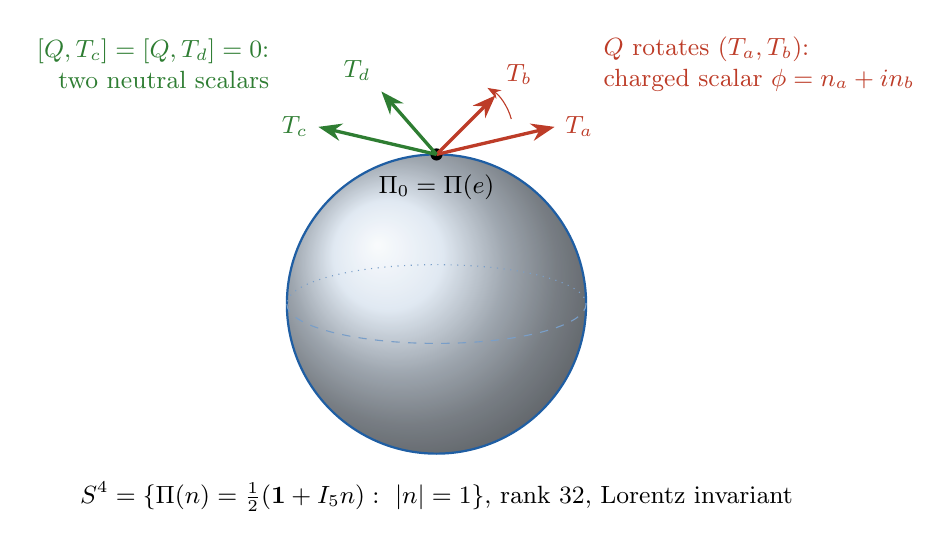
\begin{tikzpicture}[>=Stealth,font=\small]
\shade[ball color=tcol!20,opacity=0.9] (0,0) circle (1.9);
\draw[tcol,thick] (0,0) circle (1.9);
\draw[tcol!60,dashed] (-1.9,0) arc (180:360:1.9 and 0.5);
\draw[tcol!60,dotted] (1.9,0) arc (0:180:1.9 and 0.5);
\coordinate (N) at (0,1.9);
\fill[black] (N) circle (2.2pt);
\node[anchor=north,yshift=-4pt] at (N) {$\Pi_0=\Pi(e)$};
\draw[->,scol,very thick] (N) -- ++(1.5,0.35) node[right] {$T_a$};
\draw[->,scol,very thick] (N) -- ++(0.75,0.75) node[above right] {$T_b$};
\draw[scol,->] (0.95,2.35) arc (15:60:0.65);
\node[scol,anchor=west,align=left] at (2.0,3.05) {$Q$ rotates $(T_a,T_b)$:\\ charged scalar $\phi=n_a+in_b$};
\draw[->,gcol,very thick] (N) -- ++(-1.5,0.35) node[left] {$T_c$};
\draw[->,gcol,very thick] (N) -- ++(-0.7,0.8) node[above left] {$T_d$};
\node[gcol,anchor=east,align=right] at (-2.0,3.05) {$[Q,T_c]=[Q,T_d]=0$:\\ two neutral scalars};
\node[align=center] at (0,-2.45) {$S^4=\{\Pi(n)=\tfrac12(\id+I_5n):\ |n|=1\}$, rank $32$, Lorentz invariant};
\end{tikzpicture}
\caption{The compact family of second-rung vacua (\cref{thm:S4}). Every point is a Lorentz-invariant projector; at the vacuum $\Pi_0$, which commutes with the charge $Q$,
the four tangent directions are generated by compact bivectors, two of them rotated into each other by $Q$ and two neutral.}
\label{fig:S4}
\end{figure}

\begin{theorem}[The curved extension]
\label{thm:towercurved}
Reduce the internal connection so that $a,b$ carry the normal $SO(2)$ connection and $c,d,e$ are parallel, $\Omega=\Omega_{\rm Lorentz}+AQ$. Both summands commute with
$\Pi_0$, so
\[
D\Pi_0=0,\qquad [\mathcal R,\Pi_0]=0
\]
for arbitrary spacetime curvature and arbitrary normal curvature, the two conditions that the transport obstruction of \cref{prop:obstruct} separates, here satisfied
together by construction. Throughout the family $\mathcal C_\mu=[\Pi,D_\mu\Pi]=\tfrac14[n,D_\mu n]=\tfrac12\,n\wedge D_\mu n$, a compact internal bivector at every point, so the
adapted connection stays spin-valued away from the vacuum as well.
\end{theorem}

For a general projector $[\Pi,D\Pi]$ need not be a bivector: in a normal frame with unit clock $w$ and negative $s,t$, the projector $\Pi=\tfrac12(\id+X)$ with $X=(w+ws)/\sqrt2$
and $B=st$ gives $[\Pi,[B,\Pi]]=\tfrac12(t-st)$, which has a grade-one part. The $S^4$ family avoids this by construction.

\begin{proposition}[The vacuum and the matter]
\label{prop:towermatter}
The stabiliser of $\Pi_0$ in the internal $\so{5,3}$ is $\so4\oplus\so{1,3}$, of dimension $12$ with compact part $\su2\oplus\su2\oplus\su2$, which does not contain $\su3$. The
construction is therefore incompatible with colour at $n=2$; it is compatible from the third rung on:
\begin{center}
\small
\begin{tabular}{@{}cccc@{}}
\toprule
rung & internal algebra & stabiliser of $H$ & compact part\\
\midrule
$n=2$ & $\so{5,3}$, $\dim28$ & $\so4\oplus\so{1,3}$, $\dim12$ & $9$, no $\su3$\\
$n=3$ & $\so{8,6}$, $\dim91$ & $\so4\oplus\so{4,6}$, $\dim51$ & $27$, containing $\so6\supset\su3$\\
$n=4$ & $\so{11,9}$, $\dim190$ & $\so4\oplus\so{7,9}$, $\dim126$ & $63$\\
\bottomrule
\end{tabular}
\end{center}
At $n=3$, the rung of $P_*$, the unbroken compact algebra is $\so4\oplus\so4\oplus\so6$ and contains colour.
\end{proposition}

The second-rung vacuum settles that a vacuum which is simultaneously Lorentz invariant, uncharged, not rigid and moved by a compact generator exists, so the first-rung
rigidity of \cref{prop:rigid} is a property of that rung and not a law; its fluctuation spectrum is one charged complex scalar and two neutral ones, its current is an
ordinary charged-scalar current, and its curved extension has $D\Pi_0=0$ with a spin-valued adapted connection across the whole family. It does not settle which point
of $S^4$ is selected, since a spectrum-only potential is constant on the family; whether $j_\Pi$ is the electric current of a fermion, with which charge normalisation;
the values of $f$ and $g_A$; stability; or a gravitational action. It must be done at $n\ge3$ to leave room for colour. And it uses the spectator action throughout:
under the mixed action of \cref{sec:mixed}, $\Pi_0$ is preserved only by the rotations about one axis, its commutators with the six mixed generators span a
five-dimensional space, and the rank-$16$ Dirac block of the coupled model meets the range of $\Pi_0$ only in zero, with $P\Pi_0P$ having eigenvalues $\tfrac14$ and $\tfrac34$
on it. What the coupled model and the second-rung vacuum share is the charge: $Q=\tfrac12J_1$.

The dichotomy left at the end of \cref{sec:transport} is thereby resolved in one direction. If the normal $U(1)$ is to be electromagnetism, the paired-mode projector
must go, and \cref{thm:towervac} shows what can replace it. At one constituent, the paired-mode projector of \cref{ex:pairedmode} fails the photon test.

\part{Causal structure}
\section{Causal structure: the six-dimensional baseline}
\label{sec:baseline}

Every construction so far has used a Lorentzian four-plane chosen inside $\R^{3,3}$: the interior plane $E$ of the Dirac structure, or the slice $\Sigma$
of the curved model. This part asks whether that choice, and with it the light cone and the distinction between past and future, can be obtained from the
split geometry rather than postulated. Two levels must be distinguished. \emph{Weak emergence} means that an already selected $3{+}1$ sector carries a
consistent quantum causal structure. \emph{Strong emergence} means that the dynamics determine why that sector, with that causal structure, arises from the
six-dimensional theory. The light cone must not be put into the admissibility conditions and then be said to emerge. We fix the failure conditions in advance:
uncontrolled growing modes in the six-dimensional theory; a projector onto the four-dimensional sector imposed by hand; ghosts or negative spectral weights in
the effective theory; propagation outside the derived cone; extra modes or imposed equations in the Maxwell sector.

\subsection{The unrestricted scalar}

\begin{proposition}[A free field on $\R^{3,3}$]
\label{prop:toy}
For the action $S_6=\tfrac12\int d^6X\,(\eta^{AB}\partial_A\phi\,\partial_B\phi-m^2\phi^2)$ in coordinates $(t,u,v,x,y,z)$, with $t,u,v$ temporal:
\begin{enumerate}[label=(\roman*),leftmargin=2.2em]
\item plane waves $e^{-i\omega t+i(q_1u+q_2v)+i\bk\cdot\mathbf x}$ obey
\begin{equation}
\label{eq:toydisp}
\omega^2=|\bk|^2+m^2-q^2,\qquad q^2=q_1^2+q_2^2 ;
\end{equation}
\item for $q^2>|\bk|^2+m^2$ the growth rate is $\gamma=\sqrt{q^2-|\bk|^2-m^2}$, and $(1+q^2)^{-s/2}e^\gamma\to\infty$ for every $s$: data small in any Sobolev norm
produce arbitrarily large solutions at $t=1$, so the Cauchy problem with respect to $t$ is ill-posed in the sense of Hadamard \cite{Hadamard23};
\item the canonical energy density $\tfrac12(\pi^2-\phi_u^2-\phi_v^2+|\nabla_{\mathbf x}\phi|^2+m^2\phi^2)$ averages to $\tfrac14a^2(m^2-q^2)$ on $\phi=a\sin qu$: the
energy is unbounded below.
\end{enumerate}
\end{proposition}

\begin{figure}[t]
\centering
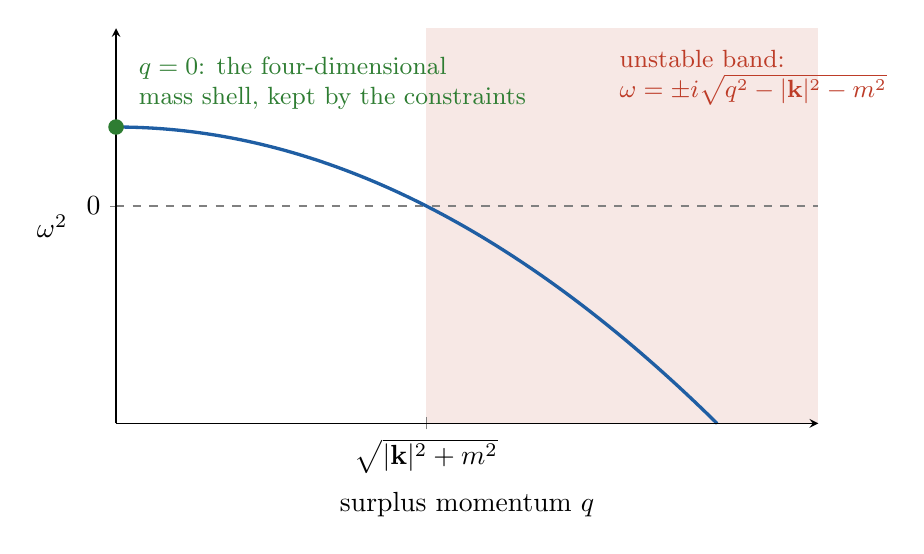
\begin{tikzpicture}
\begin{axis}[width=10.5cm,height=6.6cm,xmin=0,xmax=3.2,ymin=-5.5,ymax=4.5,axis on top,clip=false,
  axis lines=left,
  xlabel={surplus momentum $q$},ylabel={$\omega^2$},xtick={1.4142},xticklabels={$\sqrt{|\bk|^2+m^2}$},ytick={0},
  ylabel style={rotate=-90}]
\addplot[draw=none,fill=scol!12,forget plot] coordinates {(1.4142,-5.5) (3.2,-5.5) (3.2,4.5) (1.4142,4.5)} -- cycle;
\draw[gray,dashed] (axis cs:0,0) -- (axis cs:3.2,0);
\addplot[tcol,very thick,domain=0:2.739,samples=80] {2-x^2};
\addplot[only marks,mark=*,mark size=2.6pt,gcol] coordinates {(0,2)};
\node[gcol,anchor=south west,font=\small,align=left] at (axis cs:0.06,2.2) {$q=0$: the four-dimensional\\ mass shell, kept by the constraints};
\node[scol,anchor=north west,font=\small,align=left] at (axis cs:2.25,4.2) {unstable band:\\ $\omega=\pm i\sqrt{q^2-|\bk|^2-m^2}$};
\end{axis}
\end{tikzpicture}
\caption{The dispersion relation of a free scalar on $\R^{3,3}$ at fixed spatial momentum (\cref{prop:toy}). Every surplus momentum beyond $\sqrt{|\bk|^2+m^2}$ gives
an exponentially growing mode, with a rate that grows without bound. The constraints of \cref{prop:constraints} keep exactly the point $q=0$.}
\label{fig:toy}
\end{figure}

\begin{proposition}[No time orientation in signature $(3,3)$]
\label{prop:orient}
The timelike set $\{\eta(X,X)>0\}$ of $\R^{p,q}$ is connected for $p\ge2$: the path $X(s)=(\cos s,\sin s,0;\,0,0,0)$ joins $X$ to $-X$ with $\eta=1$ throughout. Only for $p=1$
does it split into a past and a future component.
\end{proposition}

Causal order is therefore not merely unproven in $\R^{3,3}$; it is absent. Anything called a light cone with a future has to come from a reduction to a single
time. The arena already contains such a reduction, as an input. For the geodesic test particle of \cref{prop:constraints}, $H=\tfrac12(h^{\mu\nu}k_\mu k_\nu+p_u^2+p_v^2)$
with $h=\operatorname{diag}(1,-1,-1,-1)$, the mass shell $2H=m^2$ is $p_0^2=|\mathbf p|^2+m^2-p_u^2-p_v^2$, the relation \eqref{eq:toydisp} with $q=(p_u,p_v)$. The
first-class constraints $p_u=p_v=0$ remove exactly the unstable band, as \cref{fig:toy} shows.

\begin{example}[Compact surplus times give tachyons]
\label{ex:tachyons}
If instead $u$ and $v$ are made periodic with period $2\pi R$, the surplus momenta become $n/R$ with $n\in\Z^2$, and the four-dimensional masses are
\[
m_n^2=m^2-\frac{|n|^2}{R^2}.
\]
Every mode with $|n|>mR$ is a tachyon, and there are infinitely many: for $mR=3$ there are $92$, $412$ and $1652$ of them within $|n_i|\le5$, $10$ and $20$.
Compactification, the usual cure for extra space dimensions, is no cure for extra times.
\end{example}

An ultrahyperbolic problem can be made well posed by a nonlocal constraint on the data \cite{CraigWeinstein09}, and the dimensionality of spacetime has been
argued from such considerations \cite{Tegmark97}. The constraints of the arena, $\partial_u\phi=\partial_v\phi=0$, are local and stronger: they keep only the zero modes,
which is dimensional reduction. Either way the cure is a restriction, and at this stage it is an input. \Cref{sec:constraints} asks where it can come from; the next
two sections ask whether the four-plane it presupposes can be selected.

\section{The kinematic selector}
\label{sec:selector}

Choosing a Lorentzian four-plane inside $\R^{3,3}$ is equivalent to choosing its orthogonal complement, a two-plane, and a two-plane is described by its unit
bivector. The question is which bivectors describe a Lorentzian complement, and what the arena does with them.

\subsection{One constituent}

\begin{theorem}[The selector is a complex structure]
\label{thm:selector}
Let $C=a\wedge b$ be a simple bivector of $\R^{3,3}$ and $N=\langle a,b\rangle$.
\begin{enumerate}[label=(\roman*),leftmargin=2.2em]
\item $C^2=-\det\mathrm{Gram}(a,b)\,\id$.
\item For a nondegenerate $N$ with $C$ normalised: $C^2=-\id$ exactly when $N$ is definite, that is exactly when $N^\perp$ is Lorentzian, of signature $(1,3)$
when $N$ is positive and $(3,1)$ when $N$ is negative; $C^2=+\id$ exactly when $N^\perp$ has signature $(2,2)$; and $C^2=0$ exactly when $N$ is degenerate.
\item The centraliser of $C$ in $\so{3,3}$ is $\so N\oplus\so{N^\perp}$, of dimension seven, so the choices of $N$ of a given type form an eight-dimensional homogeneous
space.
\item The surplus plane is such an $N$, with $C=J=e_2e_3$ and $N^\perp$ the interior four-plane.
\end{enumerate}
\end{theorem}

\begin{proof}
(i) is the Clifford identity $(a\wedge b)^2=(a\cdot b)^2-a^2b^2$. (ii) For an orthonormal pair, $(ab)^2=-a^2b^2$, which is $-1$ when $a^2=b^2$ and $+1$ otherwise, and the
signature of $N^\perp$ is the complement of that of $N$ in $(3,3)$. (iii) holds for coordinate planes by \eqref{eq:bladecomm}, and every nondegenerate plane is an
$SO(3,3)$-image of a coordinate plane of the same signature, by Witt's theorem.
\end{proof}

For coordinate planes $C$ is moreover antisymmetric on $S$ when $C^2=-\id$, an orthogonal complex structure; for tilted planes it is not. Orthogonality refers to the
Euclidean structure of $S$, which singles out the temporal triple, while $C^2=-\id$ is invariant. The distinction will matter.

Spinors give the light cone. The volume element $\omega_S=e_4e_5e_6$ satisfies $\omega_Se_A\omega_S^{-1}=-e_A^{\!\top}$ for every generator, so
$\langle\psi,\varphi\rangle=\psi^{\!\top}\omega_S\varphi$ is a $\mathrm{Spin}(3,3)$-invariant pairing, and it pairs $S^+$ with $S^-$.

\begin{theorem}[The light cone as twisted squares]
\label{thm:cone}
Let $\psi$ range over the chiral half $S^+$.
\begin{enumerate}[label=(\roman*),leftmargin=2.2em]
\item The forms $m_A=\omega_Se_A$ are antisymmetric and satisfy $X^{\!\top}m_A+m_AX=-\omega_S[X,e_A]$ for every bivector $X$; their restrictions to $S^+$ span
$\Lambda^2(S^+)^*$, so $\psi\wedge\varphi\mapsto(\psi^{\!\top}\omega_Se_A\varphi)_A$ is an equivariant isomorphism $\Lambda^2S^+\cong\R^{3,3}$, the Klein correspondence of
\cref{thm:klein}.
\item On $S^+$, $J^2=-\id$, so $S^+\cong\C^2$, and the interior $\so{1,3}$ acts $\C$-linearly, as $\slr{2,\C}$.
\item For a unit simple bivector $C$ with plane $N$ define $v_C(\psi)_A=\psi^{\!\top}\omega_Se_AC\psi$. Then $v_C(\psi)\in N^\perp$ and $\eta(v_C,v_C)=0$ identically,
and the image has dimension three.
\item If $C^2=-\id$, the component of $v_C$ along the timelike direction of $N^\perp$ is definite: $v_C$ fills one nappe of the light cone of $N^\perp$. If
$C^2=+\id$, no component is definite, and $v_C$ fills the null vectors of a $(2,2)$ plane, which has no time orientation.
\item $v_{-C}=-v_C$; on $S^-$ the $J$-twisted square lies in the other nappe; and on $S^+$, $v_J=-j$, where $j_A=\psi^{\!\top}\gamma^0e_A\psi$ is the Dirac current.
\end{enumerate}
\end{theorem}

\begin{figure}[t]
\centering
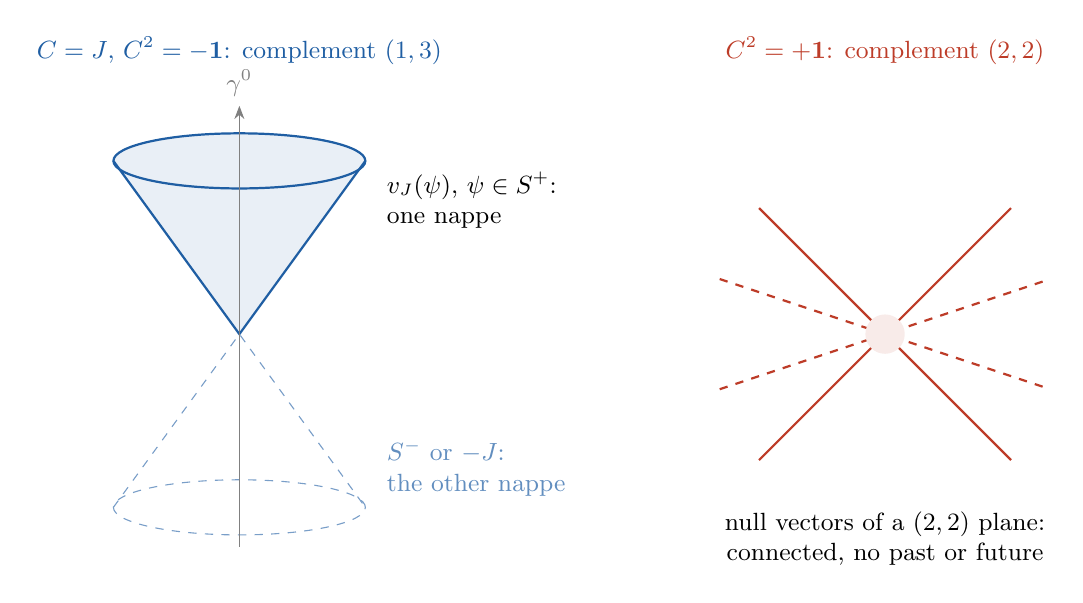
\begin{tikzpicture}[>=Stealth,font=\small]
\begin{scope}
\fill[tcol!10] (0,0) -- (1.6,2.2) arc (0:180:1.6 and 0.35) -- cycle;
\draw[tcol,thick] (-1.6,2.2) -- (0,0) -- (1.6,2.2);
\draw[tcol,thick] (0,2.2) ellipse (1.6 and 0.35);
\draw[tcol!60,dashed] (-1.6,-2.2) -- (0,0) -- (1.6,-2.2);
\draw[tcol!60,dashed] (0,-2.2) ellipse (1.6 and 0.35);
\draw[->,gray] (0,-2.7) -- (0,2.9) node[above] {$\gamma^0$};
\node[tcol,align=center] at (0,3.6) {$C=J$, $C^2=-\id$: complement $(1,3)$};
\node[anchor=west,align=left] at (1.75,1.7) {$v_J(\psi)$, $\psi\in S^+$:\\ one nappe};
\node[anchor=west,align=left,tcol!70] at (1.75,-1.7) {$S^-$ or $-J$:\\ the other nappe};
\end{scope}
\begin{scope}[xshift=8.2cm]
\draw[scol,thick] (-1.6,-1.6) -- (1.6,1.6); \draw[scol,thick] (-1.6,1.6) -- (1.6,-1.6);
\draw[scol,thick,dashed] (-2.1,-0.7) -- (2.1,0.7); \draw[scol,thick,dashed] (-2.1,0.7) -- (2.1,-0.7);
\fill[scol!10] (0,0) circle (0.25);
\node[scol,align=center] at (0,3.6) {$C^2=+\id$: complement $(2,2)$};
\node[align=center] at (0,-2.6) {null vectors of a $(2,2)$ plane:\\ connected, no past or future};
\end{scope}
\end{tikzpicture}
\caption{The selector at one constituent (\cref{thm:selector,thm:cone}). A unit bivector $C$ with $C^2=-\id$ selects a Lorentzian complement, and the $C$-twisted squares of
chiral spinors fill one nappe of its light cone, the other nappe belonging to the other chirality or to $-C$. A bivector with $C^2=+\id$ selects a $(2,2)$ complement,
whose null set has no time orientation.}
\label{fig:selector}
\end{figure}

The selector of the reduction is therefore not a new field. Choosing the spacetime $N^\perp$ and choosing the complex structure $C$ are one choice, and in the arena that
complex structure is the charge $J$, the same $J$ that is the imaginary unit of the Dirac theory (\cref{thm:i}). Null directions are the squares of Weyl spinors twisted
by $J$, and the time orientation is fixed by the sign of $J$ together with the chirality. The mathematics is the Klein--Penrose correspondence, in which a null vector is
$\psi\bar\psi$ \cite{PenroseRindler84,WardWells}; what is specific to the arena is that $J$ already plays this role. All of this is kinematics: nothing yet says why $J$,
rather than an indefinite or degenerate bivector, is chosen. For degenerate planes $v_C$ is still null with a three-dimensional image, and for the totally null plane
$\langle e_1+e_4,e_2+e_5\rangle$ it lies in the totally null three-plane $\langle e_i+e_{i+3}\rangle$, an eigenspace of the grading root $\cK$.

\subsection{Three constituents}

At three constituents $J$ is the product of the fourteen generators of the Lorentz complement $W_3$, of signature $(8,6)$, and $\Omega$ is the volume element of $E$.

\begin{theorem}[The selector at three constituents]
\label{thm:selector3}
\begin{enumerate}[label=(\roman*),leftmargin=2.2em]
\item $J^2=\Omega^2=-\id$, $[J,\Omega]=0$ and $\Gamma=J\Omega$ with $\Gamma^2=\id$; $\Omega=-J$ on $\Gamma=+1$. Since $\Gamma^2=\id$ at every rung, any coordinate four-plane $E'$
with volume element $\Omega_{E'}$ and complementary volume element $J_{E'}$ has $J_{E'}^2=\Omega_{E'}^2=\prod_{i\in E'}e_i^2$: the volume element of the complement is a complex
structure exactly when $E'$ is Lorentzian, at every $n$.
\item The centraliser of $J$ among the $153$ bivectors has dimension $97=6+91$, so the choices form a space of dimension $56$.
\item With either $\mathrm{Spin}(9,9)$-invariant pairing, the product $\beta_{\rm odd}$ of the nine negative generators, which is antisymmetric, or the product $\beta_{\rm even}$
of the nine positive ones, which is symmetric, $\beta e_AJ$ is symmetric exactly for the fourteen directions of $W_3$: the $J$-twisted square lives on the complement,
not on $E$. The untwisted $\beta_{\rm odd}e_A$ is symmetric for all eighteen directions, so the vector sits in $\mathrm{Sym}^2S^+$, and at random spinors the untwisted
square is not null.
\end{enumerate}
\end{theorem}

The identification of the selector with $J$ survives at three constituents, but the covariant construction of the cone from spinors is a feature of dimension six. At
$n=3$ the cone of $E$ is recovered by the Dirac current $j_\mu=\psi^{\!\top}\gamma^0\gamma_\mu\psi$, which is future causal, being a sum of one-constituent currents, and
null on product states; but it uses the clock $\gamma^0$ and the transpose, that is, the positive inner product of the spinor module.

\section{Type selection}
\label{sec:typesel}

Kinematics identifies the selector with a complex structure. Dynamics would have to explain why the field that plays this role takes a value of the
complex-structure type at all, rather than an indefinite or degenerate one. The natural test is a potential: take the order parameter to be a bivector field
$B\in\so{3,3}$, ask that the potential be invariant under $SO(3,3)$, so that nothing is put in by hand, and require that its minimum set be exactly the orbit of $J$,
over an open set of couplings, with healthy fluctuations. Restriction to $S^+$ is the isomorphism $\so{3,3}\cong\slr{4,\R}$, and the invariant polynomials are the
polynomials in
\[
t_k(B)=\tr\bigl((B|_{S^+})^k\bigr),\qquad k=2,3,4,
\]
the coefficients of the characteristic polynomial; a continuous invariant function is constant on orbit closures.

\begin{proposition}[Invariants of the three types]
\label{prop:types}
Rotations of a positive plane and of a negative plane both have $(t_2,t_3,t_4)=(-4,0,4)$ and characteristic polynomial $(y^2+1)^2$; boosts of an indefinite plane have
$(4,0,4)$ and $(y-1)^2(y+1)^2$. The positive and the negative planes induce opposite orientations of $S^+=\R^4$: they are distinct $SL(4,\R)$-orbits with identical
invariants.
\end{proposition}

So no invariant potential can prefer $(1,3)$ to $(3,1)$. The two are exchanged by the anti-isometries $\cK$ and $G$ and correspond to the two sign conventions for a
Lorentzian metric; physically this is harmless, but it means the selection is never unique. The type itself is harder.

\begin{theorem}[No clean selection below degree eight]
\label{thm:degree}
Let $V$ be an $SO(3,3)$-invariant polynomial on $\so{3,3}$, bounded below.
\begin{enumerate}[label=(\roman*),leftmargin=2.2em]
\item If $\deg V\le4$, then $V=m\,t_2+\lambda\,t_2^2+\mathrm{const}$.
\item If $\deg V\le7$, then $V$ restricted to $\{t_3=0\}$ is a polynomial of degree at most two in $t_2$ alone.
\item Hence if $J$ minimises $V$, so does $B_w=\tfrac35e_2e_3+\tfrac45e_5e_6$, which has $t_2=-4$, $t_3=0$ and $t_4=\tfrac{4804}{625}\neq4$, is not simple, and selects no four-plane.
\item In degree eight, $f=(t_2+4)^2+t_3^2+(t_4-4)^2$ vanishes exactly on the elements with characteristic polynomial $(y^2+1)^2$, and its Hessian at $J$ has rank one.
\end{enumerate}
\end{theorem}

\begin{proof}
Use test elements of $\slr{4,\R}$ with rational entries. $A_0=\operatorname{diag}(1,-1)\oplus\bigl(\begin{smallmatrix}0&-1\\1&0\end{smallmatrix}\bigr)$ and
$B_0=\bigl(\begin{smallmatrix}1&-1\\1&1\end{smallmatrix}\bigr)\oplus\bigl(\begin{smallmatrix}-1&-1\\1&-1\end{smallmatrix}\bigr)$ have $t_2=t_3=0$ and $t_4=4,-16$;
$C_0=\operatorname{diag}(-1,-3)\oplus\bigl(\begin{smallmatrix}2&-3\\3&2\end{smallmatrix}\bigr)$ has $t_2=0$ and $t_3=-120$; the complex and para-complex structures have
$(t_2,t_4)=(\mp4,4)$; $D_0=\operatorname{diag}(1,-1,2,-2)$ and two rotations of speeds $1,2$ have $(t_2,t_4)=(\pm10,34)$, all with $t_3=0$. (i) Along $sA_0$ and $sB_0$ a quartic
term $\lambda_2t_4$ would give $\lambda_2t_4s^4$ with both signs of $t_4$, so $\lambda_2=0$ for boundedness; along $sC_0$ a cubic term gives $-120\kappa s^3$, so $\kappa=0$. (ii) The top
homogeneous part must be non-negative, so an odd top degree vanishes, and in degree six the top part $e\,t_2^3+f\,t_3^2+g\,t_2t_4$ takes the values $\mp(64e+16g)$ on the
complex and para-complex structures and $\pm(1000e+340g)$ on the last two elements; non-negativity forces $g=-4e$ and then $e=g=0$, with $f\ge0$ from $C_0$. The quartic
coefficient of $t_4$ must again vanish, leaving $a\,t_2+b\,t_3+c\,t_2^2+h\,t_2t_3+f\,t_3^2$, which on $t_3=0$ is $a\,t_2+c\,t_2^2$. (iii) follows. (iv) $f\ge0$ with equality exactly
when $(t_2,t_3,t_4)=(-4,0,4)$, which fixes the characteristic polynomial by Newton's identities; at $J$ the gradients of $t_3$ vanish and those of $t_2$ and $t_4$ are
proportional, so the Hessian has rank one.
\end{proof}

\begin{figure}[t]
\centering
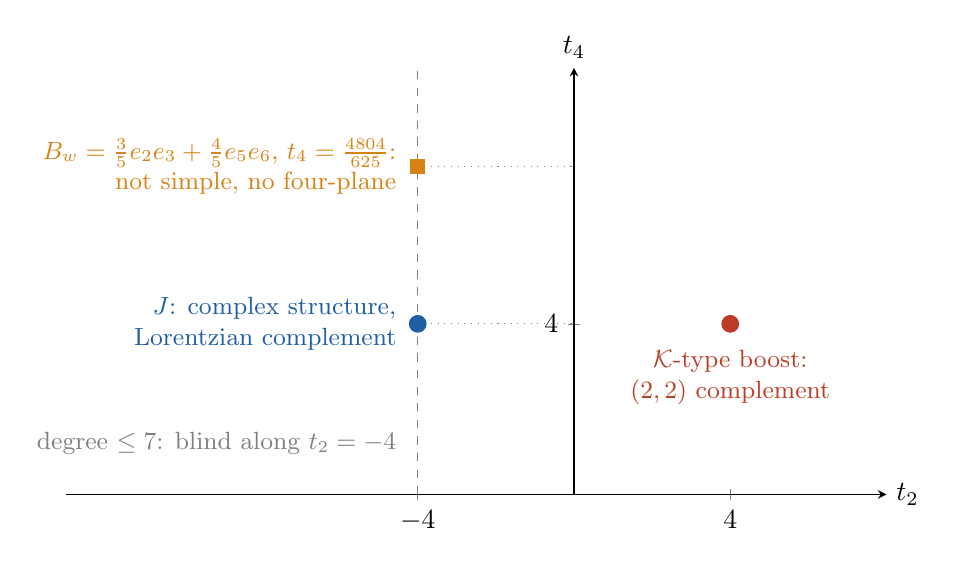
\begin{tikzpicture}
\begin{axis}[width=12cm,height=7cm,xmin=-13,xmax=8,ymin=0,ymax=10,axis lines=middle,clip=false,
  xlabel={$t_2$},ylabel={$t_4$},xtick={-4,4},ytick={4},
  xlabel style={anchor=west},ylabel style={anchor=south}]
\draw[gray,dashed] (axis cs:-4,0) -- (axis cs:-4,10);
\draw[gray,dotted] (axis cs:-4,4) -- (axis cs:0,4);
\draw[gray,dotted] (axis cs:-4,7.6864) -- (axis cs:0,7.6864);
\addplot[only marks,mark=*,mark size=3pt,tcol] coordinates {(-4,4)};
\addplot[only marks,mark=*,mark size=3pt,scol] coordinates {(4,4)};
\addplot[only marks,mark=square*,mark size=2.6pt,ocol] coordinates {(-4,7.6864)};
\node[tcol,anchor=east,font=\small,align=right] at (axis cs:-4.3,4) {$J$: complex structure,\\ Lorentzian complement};
\node[scol,anchor=north,font=\small,align=center] at (axis cs:4,3.6) {$\cK$-type boost:\\ $(2,2)$ complement};
\node[ocol,anchor=east,font=\small,align=right] at (axis cs:-4.3,7.69) {$B_w=\tfrac35e_2e_3+\tfrac45e_5e_6$, $t_4=\tfrac{4804}{625}$:\\ not simple, no four-plane};
\node[gray,anchor=east,font=\small] at (axis cs:-4.3,1.2) {degree $\le7$: blind along $t_2=-4$};
\end{axis}
\end{tikzpicture}
\caption{Type selection in the plane of the invariants $(t_2,t_4)$ at $t_3=0$ (\cref{thm:degree}). A bounded-below invariant potential of degree at most seven depends on $t_2$
alone along $t_3=0$, so it cannot distinguish the complex structure $J$ from the non-simple element $B_w$ on the same vertical line. Degree eight is the first that can.}
\label{fig:typesel}
\end{figure}

Even where a potential does isolate the type, the minimum cannot be clean, and the reason holds at every degree.

\begin{theorem}[Degeneracy and flat directions at every degree]
\label{thm:flat}
Let $V$ be any $SO(3,3)$-invariant function on $\so{3,3}$.
\begin{enumerate}[label=(\roman*),leftmargin=2.2em]
\item Let $n=(e_1+e_4)e_5$, a null rotation of the interior four-plane. Then $[J,n]=0$ and $n^2=0$, so $J+n$ has the invariants of $J$, but its centraliser has dimension three
and does not contain $\so{1,3}$: it breaks Lorentz invariance. With $K=\tfrac12e_1e_4$, $[K,n]=-n$ and $[K,J]=0$, so conjugation by $e^{tK}$ maps $J+n$ to $J+e^{-t}n$. Hence $J$
lies in the closure of the orbit of $J+n$, and $V(J+n)=V(J)$ whenever $V$ is continuous.
\item If $V$ is smooth and has a local minimum at $J$, its Hessian vanishes on the six $\so{1,3}$ directions. The $\Stab(J)$-invariant symmetric forms on $\so{1,3}$ are the real
and imaginary parts of the complex Killing form of $\slr{2,\C}$, and each nonzero one has signature $(3,3)$, so a positive semidefinite one is zero.
\end{enumerate}
At best the fluctuations about $J$ are one massive radial mode, eight Goldstone modes and six massless modes that no symmetry protects.
\end{theorem}

\begin{proposition}[Kinetic terms]
\label{prop:kineticB}
$\so{3,3}$ is simple, so every $SO(3,3)$-invariant quadratic kinetic term is a multiple of the Killing form, which on the fifteen bivectors has signature $(9,6)$, boosts with
one sign and rotations with the other. At $J$ the radial direction is a rotation, the eight Goldstone directions are two rotations and six boosts, and the six $\so{1,3}$
directions are three of each. Whatever the overall sign, at least six directions are ghosts, and the induced metric on the eight-dimensional space of choices has
signature $(6,2)$.
\end{proposition}

In covariant terms the Goldstone directions form a charged four-vector and the $\so{1,3}$ directions a two-form, and healthy vectors and two-forms owe their positivity to a
gauge symmetry that removes the wrong-sign components; a scalar order parameter has none. This is \cref{thm:ghost} again, in a new setting. There is a positive
alternative, and it shows what is missing.

\begin{proposition}[The positive alternative]
\label{prop:positivealt}
On the fifteen bivectors the positive form $\langle X,Y\rangle=\tr(XY^{\!\top})/8$ is the identity, and its invariance algebra is the six compact rotations $\so3_T\oplus\so3_S$.
Split $B=B_T+B_S+B_p$ into these two parts and the nine boosts. The potential
\[
V_+=\bigl(|B_T|^2-1\bigr)^2+|B_S|^2+|B_p|^2
\]
has as minimum set the unit sphere of $\so3_T$. Every element there is a rotation of a plane $N$ in the temporal triple, the clock is the axis of the rotation, the spacetime is the
clock line plus the spatial triple, and $J=\gamma^0\omega_T$. The Hessian at $J$ has eigenvalues $8$, $0$, $0$ and $2$ (twelve times): two Goldstone modes and everything else massive
with positive kinetic energy. But the boosts $e_1e_4,e_1e_5,e_1e_6$ of the selected spacetime are not symmetries of this sector.
\end{proposition}

The requirement was a clean selection of the Lorentzian type over an open set of couplings, with every mode healthy and accounted for. An $SO(3,3)$-invariant scalar
order parameter cannot deliver it: below degree eight it does not isolate the type; at every degree the minimum is degenerate with Lorentz-violating configurations and has
six unprotected massless modes; and its kinetic term has ghosts. The positive route selects cleanly only by giving up the boosts it was meant to produce.

\section{Where the surplus constraints come from}
\label{sec:constraints}

The baseline showed that the constraints $p_u=p_v=0$ remove exactly the unstable band, and the curved model showed that they are first class. A first-class constraint
generates a gauge symmetry, so the question is which symmetry, and whether it is a natural one.

\begin{theorem}[A worldline gauge symmetry]
\label{thm:wlgauge}
For arbitrary $A_\mu(x)$ and flat $h$, with $C=A_\mu h^{\mu\nu}k_\nu$, the constraints satisfy $\{p_u,H\}=-Cp_v$, $\{p_v,H\}=Cp_u$, $\{p_u,p_v\}=0$ and $\{\ell,H\}=0$. The extended action
\[
\int d\tau\,\bigl(p\cdot\dot x-NH-\lambda_1p_u-\lambda_2p_v\bigr)
\]
is invariant under
\[
\delta u=\varepsilon_1(\tau),\qquad \delta v=\varepsilon_2(\tau),\qquad \delta\lambda_1=\dot\varepsilon_1+NC\varepsilon_2,\qquad \delta\lambda_2=\dot\varepsilon_2-NC\varepsilon_1,
\]
all other variables fixed: local translations along the normal plane, which are gauge symmetries although they are not isometries when $F\neq0$, the algebra closing with
structure functions \cite{HenneauxTeitelboim92}. In Dirac quantisation the physical states are the functions $\Psi(x)$ on spacetime, and on them $\hat H\Psi=-\tfrac12\Box_h\Psi$;
the potential $A$ drops out.
\end{theorem}

\begin{proposition}[Gauging the isometry is not enough]
\label{prop:isometryonly}
In polar normal coordinates $\ell=-p_\phi$ and $p_u^2+p_v^2=p_r^2+p_\phi^2/r^2$. Gauging only the rotation $\ell$, the isometry of the normal plane, leaves
$p_0^2=|\mathbf p|^2+m^2-p_r^2$: the radial surplus momentum keeps the unstable band. For fields, the rotation-invariant modes $J_0(qr)e^{-i\omega t+i\bk\cdot\mathbf x}$ obey
$\omega^2=|\bk|^2+m^2-q^2$.
\end{proposition}

The symmetry that removes the instability is therefore the full group of local translations along the normal plane, not its rotation subgroup.

\begin{corollary}[Weak emergence for scalar matter]
\label{cor:weak}
If the normal translations are gauged, the scalar sector reduces to the Klein--Gordon field on $(M^4,h)$: its energy is bounded below, its evolution is unitary, and
$[\phi(x),\phi(y)]=0$ at spacelike separation for the cone of $h$ \cite{WeinbergQFT}. In the free theory the zero modes $\psi$ and the surplus modes $\chi$ do not mix, since
translation invariance along the normal plane makes the mixed kernel $K_{\psi\chi}$ vanish, so the Schur complement is trivial and $K_{\rm eff}=K_{\psi\psi}$; the content is not in
the kernel but in whether $\chi$ is physical, and under the gauge principle it is not. The causal cone is that of $h$, the metric of the selected four-plane: it is inherited
from the reduction, not derived from the six-dimensional sum.
\end{corollary}

What the reduction leaves over is the geometry of the normal plane itself, and it is not healthy.

\begin{theorem}[Every normal-plane vector is a ghost]
\label{thm:ghostvec}
For $ds^2=h+\sigma\bigl[(du+B^u)^2+(dv+B^v)^2\bigr]$ with flat $h$, $B^u=b_1x^1dx^2$ and $B^v=b_2x^0dx^3$, one finds $R_6=-\tfrac\sigma4\sum F_{\mu\nu}F^{\mu\nu}$, and for the
rotation ansatz $B^u=vA$, $B^v=-uA$, $R_6=-\sigma\,r^2F^2/4$, which at $\sigma=+1$ is the ambient scalar curvature of \cref{thm:ein6}. The coefficient is odd in $\sigma$, so the
healthy sign is that of a normal plane of the sign of space, $\sigma=-1$, the ordinary Kaluza--Klein case. By \cref{thm:selector}(ii) the normal plane of a Lorentzian
four-plane in $\R^{3,3}$ always has the sign of time. Every Kaluza--Klein vector from the normal plane, from its translations or its rotation, therefore gravitates with the
wrong sign, and by \cref{thm:wlgauge} none of them couples to spinless matter.
\end{theorem}

The failure condition ``ghosts or negative spectral weights'' is therefore met by the normal-plane vectors, and the photon cannot come from them. If the Maxwell field
emerges, it must come from elsewhere: from the univectorial potential of the interior reading, or from the field-strength reading $\R^{3,3}=\Lambda^2\R^{1,3}$, where the
energy is the positive Hermitian form $|\bB|^2+|\bE|^2$ (\cref{sec:spin}).

\subsection{What the causal analysis establishes}

\Cref{tab:causal} collects the outcome against the failure conditions fixed at the start of \cref{sec:baseline}.

\begin{table}[t]
\centering
\small
\begin{tabular}{@{}>{\raggedright\arraybackslash}p{2.3cm}>{\raggedright\arraybackslash}p{6.6cm}>{\raggedright\arraybackslash}p{5.1cm}@{}}
\toprule
stage & result & verdict\\
\midrule
baseline & growing modes and no ground state; exactly the band the surplus constraints remove; compactification makes tachyons & obstruction confirmed, cure located\\
reduction & kinematics: selector $=J$, cone $=$ twisted squares at one constituent; dynamics: no $SO(3,3)$-invariant scalar mechanism; the positive route breaks the boosts &
kinematics exact; dynamical selection fails as posed\\
effective theory & scalar matter: no mixing, $K_{\rm eff}=K_{\psi\psi}$; normal-plane vectors are ghosts & failure condition met by the vectors\\
causality & the scalar sector is microcausal for the cone of $h$ & conditional on gauged translations; inherited\\
Maxwell & normal-plane vectors excluded as photons & blocked on this route\\
\bottomrule
\end{tabular}
\caption{The causal analysis against the failure conditions fixed in advance (\cref{sec:baseline,sec:selector,sec:typesel,sec:constraints}).}
\label{tab:causal}
\end{table}

Weak emergence holds for scalar matter, conditionally on a gauge principle, local translations along the normal plane, that is consistent but chosen rather than derived.
Strong emergence through a scalar order parameter is excluded. What survives is a sharper statement of the question. The selector is the complex structure $J$, and every
construction here that produced a healthy Lorentzian sector also used one extra datum: a positive inner product, which is the transpose of the realisation, equivalently
the temporal triple. Within these computations the totality of $SO(3,3)$-invariant dynamics fixes at most the type of the structure, never the instance, and it fixes even
the type only imperfectly. The datum that singles out time, wherever things worked, is the positivity of an inner product; in quantum mechanics it is the positivity of
the Hilbert-space norm. That is where a derivation of causal order from the split geometry would have to look.

Several routes remain open. A gauge mechanism for type selection, an $SO(3,3)$ analogue of the MacDowell--Mansouri and Stelle--West breaking
\cite{MacDowellMansouri77,StelleWest80}, $SO(3,3)\to SO(2)\times SO(1,3)$, would make the would-be ghosts gauge, solder the eight broken directions to the base and remove the six
flat ones. A principle that makes the normal translations gauge, rather than adding the multipliers by hand, would turn weak emergence from a conditional statement into a
derived one. At three constituents, a $\mathrm{Spin}(9,9)$-covariant construction of the cone of $E$, for which pure spinors are the natural candidates, or a proof that
none exists without the positive inner product, would settle whether the cone survives the tower.

\part{Assessment}
\section{What the algebra decides}
\label{sec:assessment}

We sort the results of this paper into the four classes announced in \cref{sec:deflation}, and then name the choices that remain. The test applied throughout is the
deflationary one of \cref{cor:nopredict}: a statement about the arena carries information only if it could have come out otherwise, and compatible representation
data is not a prediction.

\subsection{Fixed by the algebra}

At one constituent the algebra fixes more than one might expect. The signature rule separates the bivectors that can gauge from those that can only grade, and the
pole operators grade the algebra by $\Z_2^3$ through a maximally split Cartan subalgebra. The pairing of the two triples has exactly two square roots, the grading root
$\cK$ and the binding root $G$, related by the Cartan involution $\Ad_{e_1e_2e_3}$. Under permutation symmetry the clock is the barycentre of the Fisher--Rao octant, and
exactly that clock makes the conversion invisible in the equations of motion. The imaginary unit is selected, not adjoined: inside the joint commutant of the interior
Lorentz action and the internal bivectors the only complex structures commuting with the gamma matrices are $\pm J$. Charge conjugation is the surplus plane, time reversal
squares to $-\id$, the kinetic forms alone fix the massless gauge algebra $\uu1_\Omega\oplus\su2$, the mass form cuts it to $\uu1_J$, and that $\uu1$ is the whole internal
centraliser. Along the tower the internal centraliser is $\so{3n-1,3n-3}$, nested and over one Lorentz frame, and the diagonal Lorentz action gives a compact internal algebra
forming a reductive dual pair with the Lorentz algebra, with the exact identity $C_{\rm cop}+C_\Delta=\tfrac12n(n+2)$.

In the field-strength reading the centraliser of $G$ is a Lorentz algebra under which $\R^{3,3}$ \emph{is} $\Lambda^2\R^{1,3}$, $G$ is the Hodge star, the two Maxwell
invariants are the real and imaginary parts of one holomorphic quadratic form, and covariance fixes the form of Maxwell's equations through a multiplicity count. In the
interior dynamics, factorisation and binding coexist exactly in neutral signature, and the force law closes in one way only, into a rotor acting by $G$ whose free motion is a
pendulum in the duality angle. In the curved arena the curvature operator lives on the frame, the first Bianchi identity is the single trace $\Tr(G\cR)=0$, and the duality
rotation of the curvature ends, where conservation and variationality both select it, at the double dual contracting to the Einstein tensor; in first-order form the same
rotation is a Barbero--Immirzi angle. Kinematically, choosing a Lorentzian four-plane is choosing a complex structure, and at one constituent the light cone is the set of
chiral spinors squared with the help of $J$.

\subsection{Constructed}

The constructions are existence results; in each case the algebra admits the object and nothing selects it among alternatives. At three constituents the axial projector
$P_*$ of rank $64$ carries the Pati--Salam algebra and one chiral family with a right-handed neutrino, and settles the question of colour with chirality. The diagonal Dirac
block carries a gauge-invariant real $\Cl(1,3)$ built from a copy-singlet cubic. At the mixed second rung the univectorial potential, a Dirac block and the frame field can
be coupled into two-flavour spinor electrodynamics. On the $272$ mass kernels of the chiral block the renormalizable potential of the $(\mathbf{10},\mathbf1,\mathbf3)$ component
is classified, the conditions under which the Standard-Model orbit is its global minimum are found, and the radiative spectrum of all $271$ angular modes is computed, with
the electroweak stage, the seesaw and the Georgi--Jarlskog factor as consequences of a bidoublet vacuum value. At the second rung a Lorentz-invariant, uncharged, non-rigid
vacuum with a charged-scalar current exists on a compact $S^4$ of projectors, with a curved extension in which it is parallel. Both readings of $\R^{3,3}$ construct the
Einstein tensor of a given four-metric.

\subsection{Obstructed}

Each obstruction holds under hypotheses stated where it was proved, and those hypotheses are part of the result. Hypercharge cannot be read off anomaly cancellation for
charges built from three commuting involutions; $\su3$ fits in the effective algebra of no axial projector of the five-projector family; the two central $\uu1$s of $P_*$
cannot be gauged on its matter; the diagonal sector is vector-like on its complete blocks. The two readings of the same six directions exclude one another, and the
obvious repair at the second rung costs the whole internal algebra. The positive-form interior oscillates only at zero momentum. No Lie--Poisson closure lives on the frame
alone, and no inertia is both Lorentz invariant and rate-conserving. Non-orthogonality of $\bE$ and $\bB$ breaks $P$ and $T$, is never spontaneous, and generates no mass.
The paired-mode projector sources only a massive vector, and at the first rung a vacuum that is both massless and Lorentz invariant is rigid. The normal $U(1)$ of the curved
model fails as electromagnetism on three independent counts: a spinless particle cannot see it, its adapted generator does not commute with the physical generators, and it
gravitates with the wrong sign. Ricci flow does not transfer to split signature. No vacuum value of a field built from the internal bivectors and $J$ makes the matter
chiral, Hermitian order parameters keep rank five, and vacuum alignment does not see chirality. In the causal analysis, the six-dimensional free field is ill-posed and has
no time orientation, no $SO(3,3)$-invariant scalar potential of degree below eight isolates the Lorentzian type, every such potential is degenerate with a Lorentz-violating
orbit and has six unprotected flat directions, every invariant kinetic term has ghosts, and every vector from the normal plane is a ghost.

\subsection{Open, and the choices that remain}

\Cref{tab:choices} lists the choices that the algebra leaves free, with the place where each enters. Most of the open problems are downstream of them.

\begin{table}[t]
\centering
\small
\begin{tabular}{@{}>{\raggedright\arraybackslash}p{4.0cm}>{\raggedright\arraybackslash}p{10.4cm}@{}}
\toprule
choice & status\\
\midrule
the projector & a field with a computable configuration space; at rank $64$ at least two admissible orbits, of dimensions $34$ and $20$; a spectrum-only potential is constant on
them, so selection needs couplings that distinguish orbits\\
the Lorentz action & spectator and diagonal actions are not conjugate and trade against each other: a large internal algebra with ghost-signed directions and a chiral block,
or a small compact algebra on vector-like matter\\
the hypercharge direction & a compatible embedding exists on $P_*$ and is output by the vacuum of the kernel field, but the vacuum itself is selected only on an open set of
couplings\\
the binding operator and its reading & $G$ is adopted; conditional uniqueness once its Lorentz algebra is taken, not selection; the field-strength reading and the interior reading
of the same six directions exclude one another\\
scales and inertias & no ratio among the rotor inertia, the frame inertia and the coupling scales is fixed; the inertia of the closure has $21$ free directions satisfying neither
requirement\\
the action & no parent action is derived; the gauge field, the metric and the kernel field are given dynamics by adopted actions whose equations follow\\
the four-plane and positivity & the selector is $J$; the type is not selected by invariant dynamics, and every healthy construction used a positive inner product\\
families & the block carries one family; three copies of a module are a multiplicity index, not three constituents, and nothing reduces the copy multiplicity to three\\
\bottomrule
\end{tabular}
\caption{The choices the algebra leaves open.}
\label{tab:choices}
\end{table}

Several problems are sharply posed by the results. A coupling that distinguishes the points of the compact family of second-rung vacua, done at $n\ge3$ where colour
survives, would turn the photon construction into a selection. A finite search over non-diagonal pairings of the two Lorentz bases at the second rung and above would settle
whether the two readings of $\R^{3,3}$ can share one theory at an acceptable price. The spectrum and the index of the gauge-invariant Dirac operator of the diagonal block on
a curved base are ordinary index-theorem calculations, and a nonvanishing index would not contradict vector-likeness. The global structure of the potential on all $272$ mass
kernels, the choice between the Standard-Model vacuum and its mirror, the electroweak hierarchy, and the explicit breaking of the left-handed fermion number that the axion
bound requires are all open. A mechanism placing the interior momenta on the null cone or on the balance surface, the only places where a constant rate and a bounded frame
coexist, and the quantisation of the rotor, whose angle would then have to be related to an external time, are open. Whether the antisymmetric part of the shift is the
contorsion of an independent connection is a conjecture that is not yet type-correct. A gravitational action relating metric, pairing, connection and projector, from which
the metric would follow rather than be given, is the largest open problem of the curved arena; and in the causal analysis a gauge mechanism for type selection and a principle
that makes the normal translations gauge are the two steps from which a derivation of causal order would have to begin.

\subsection{The test, applied}

The largest gap is the same in every sector, and it is one of selection rather than absence. The gauge algebra is derived and the gauge field is not; the arena is derived
and its dynamics is not; the Einstein tensor of a given metric is constructed and the metric is not determined; the projector is a field whose equation follows once an action
is adopted, but no action is derived and none of its admissible orbits is singled out; the vacuum of the kernel field is selected, but only on a stated open set of couplings
and with field content given. Recovering the hypercharge table, the anomaly conditions or $\sin^2\theta_W=\tfrac38$ is a consistency result, not evidence, since any construction
with that charge content gives them. New mathematics would be a theorem that removes one of the choices of \cref{tab:choices} without adding another; new physics would require
a selected spectrum, a coupling or scale relation, a mass restriction, or a deviation that survives re-expression in the complex language of \cref{thm:realification}. None of
these is claimed here. What the paper does claim is a precise map of where the split-signature Clifford algebra decides and where it leaves the decision to the physicist,
and on that map the decided territory is larger, and its borders sharper, than one might have guessed from the size of the arena.

\appendix
\crefalias{section}{appendix}
\section{The explicit realisation}
\label{app:realisation}

Every finite-dimensional statement of this paper is a statement about integer matrices, and this appendix collects the data needed to check any of them by hand.

\paragraph{One constituent.} Label the basis of $S=\R^8=(\R^2)^{\otimes3}$ by bit strings $b=b_1b_2b_3$, ordered as the binary numbers $0,\dots,7$, and write $\delta_i$ for
the string with a single $1$ in position $i$. The generators \eqref{eq:realisation} act by
\[
e_i\,|b\rangle=(-1)^{b_1+\cdots+b_{i-1}}\,|b\oplus\delta_i\rangle,\qquad e_{i+3}\,|b\rangle=(-1)^{b_1+\cdots+b_i}\,|b\oplus\delta_i\rangle\qquad(i=1,2,3):
\]
both $e_i$ and $e_{i+3}$ flip the $i$-th bit, and they differ only by the sign carried by that bit. As matrices, with $\bar1=-1$ and dots for zeros,
\begin{center}
\scriptsize
\setlength{\arraycolsep}{2.2pt}
\[e_1=\begin{pmatrix}\cdot&\cdot&\cdot&\cdot&1&\cdot&\cdot&\cdot\\\cdot&\cdot&\cdot&\cdot&\cdot&1&\cdot&\cdot\\\cdot&\cdot&\cdot&\cdot&\cdot&\cdot&1&\cdot\\\cdot&\cdot&\cdot&\cdot&\cdot&\cdot&\cdot&1\\1&\cdot&\cdot&\cdot&\cdot&\cdot&\cdot&\cdot\\\cdot&1&\cdot&\cdot&\cdot&\cdot&\cdot&\cdot\\\cdot&\cdot&1&\cdot&\cdot&\cdot&\cdot&\cdot\\\cdot&\cdot&\cdot&1&\cdot&\cdot&\cdot&\cdot\end{pmatrix},\quad e_2=\begin{pmatrix}\cdot&\cdot&1&\cdot&\cdot&\cdot&\cdot&\cdot\\\cdot&\cdot&\cdot&1&\cdot&\cdot&\cdot&\cdot\\1&\cdot&\cdot&\cdot&\cdot&\cdot&\cdot&\cdot\\\cdot&1&\cdot&\cdot&\cdot&\cdot&\cdot&\cdot\\\cdot&\cdot&\cdot&\cdot&\cdot&\cdot&\bar1&\cdot\\\cdot&\cdot&\cdot&\cdot&\cdot&\cdot&\cdot&\bar1\\\cdot&\cdot&\cdot&\cdot&\bar1&\cdot&\cdot&\cdot\\\cdot&\cdot&\cdot&\cdot&\cdot&\bar1&\cdot&\cdot\end{pmatrix},\quad e_3=\begin{pmatrix}\cdot&1&\cdot&\cdot&\cdot&\cdot&\cdot&\cdot\\1&\cdot&\cdot&\cdot&\cdot&\cdot&\cdot&\cdot\\\cdot&\cdot&\cdot&\bar1&\cdot&\cdot&\cdot&\cdot\\\cdot&\cdot&\bar1&\cdot&\cdot&\cdot&\cdot&\cdot\\\cdot&\cdot&\cdot&\cdot&\cdot&\bar1&\cdot&\cdot\\\cdot&\cdot&\cdot&\cdot&\bar1&\cdot&\cdot&\cdot\\\cdot&\cdot&\cdot&\cdot&\cdot&\cdot&\cdot&1\\\cdot&\cdot&\cdot&\cdot&\cdot&\cdot&1&\cdot\end{pmatrix},\]
\[
e_4=\begin{pmatrix}\cdot&\cdot&\cdot&\cdot&\bar1&\cdot&\cdot&\cdot\\\cdot&\cdot&\cdot&\cdot&\cdot&\bar1&\cdot&\cdot\\\cdot&\cdot&\cdot&\cdot&\cdot&\cdot&\bar1&\cdot\\\cdot&\cdot&\cdot&\cdot&\cdot&\cdot&\cdot&\bar1\\1&\cdot&\cdot&\cdot&\cdot&\cdot&\cdot&\cdot\\\cdot&1&\cdot&\cdot&\cdot&\cdot&\cdot&\cdot\\\cdot&\cdot&1&\cdot&\cdot&\cdot&\cdot&\cdot\\\cdot&\cdot&\cdot&1&\cdot&\cdot&\cdot&\cdot\end{pmatrix},\quad e_5=\begin{pmatrix}\cdot&\cdot&\bar1&\cdot&\cdot&\cdot&\cdot&\cdot\\\cdot&\cdot&\cdot&\bar1&\cdot&\cdot&\cdot&\cdot\\1&\cdot&\cdot&\cdot&\cdot&\cdot&\cdot&\cdot\\\cdot&1&\cdot&\cdot&\cdot&\cdot&\cdot&\cdot\\\cdot&\cdot&\cdot&\cdot&\cdot&\cdot&1&\cdot\\\cdot&\cdot&\cdot&\cdot&\cdot&\cdot&\cdot&1\\\cdot&\cdot&\cdot&\cdot&\bar1&\cdot&\cdot&\cdot\\\cdot&\cdot&\cdot&\cdot&\cdot&\bar1&\cdot&\cdot\end{pmatrix},\quad e_6=\begin{pmatrix}\cdot&\bar1&\cdot&\cdot&\cdot&\cdot&\cdot&\cdot\\1&\cdot&\cdot&\cdot&\cdot&\cdot&\cdot&\cdot\\\cdot&\cdot&\cdot&1&\cdot&\cdot&\cdot&\cdot\\\cdot&\cdot&\bar1&\cdot&\cdot&\cdot&\cdot&\cdot\\\cdot&\cdot&\cdot&\cdot&\cdot&1&\cdot&\cdot\\\cdot&\cdot&\cdot&\cdot&\bar1&\cdot&\cdot&\cdot\\\cdot&\cdot&\cdot&\cdot&\cdot&\cdot&\cdot&\bar1\\\cdot&\cdot&\cdot&\cdot&\cdot&\cdot&1&\cdot\end{pmatrix}.
\]
\end{center}
The first three are symmetric and the last three antisymmetric, as \eqref{eq:transpose} requires, and $e_ae_b+e_be_a=2\eta_{ab}\id$ is checked entry by entry.

\paragraph{Derived operators at one constituent.} The pole operators are diagonal, $\omega_i\,|b\rangle=(-1)^{b_i}|b\rangle$, so their joint eigenlines are the basis lines
themselves, and the volume element is $\omega=e_1\cdots e_6=\Gamma$ with $\Gamma|b\rangle=-(-1)^{b_1+b_2+b_3}|b\rangle$; the half-spinors $S^+$ and $S^-$ are spanned by the basis
vectors with an odd, respectively even, number of ones. Further,
\[
J=e_2e_3:\ |b\rangle\mapsto(-1)^{b_2}\,|b\oplus\delta_2\oplus\delta_3\rangle,\qquad \Omega=e_1e_4e_5e_6,\qquad T=\gamma^0J=e_1e_2e_3,\qquad \Gamma=J\Omega .
\]
On $V=\R^{3,3}$ the two square roots of the pairing are
\[
\cK e_i=-e_{i+3},\quad \cK e_{i+3}=-e_i,\qquad G\,e_i=e_{i+3},\quad G\,e_{i+3}=-e_i ,
\]
with $\cK=\tfrac12\ad_{\mathsf P}$, $\mathsf P=\sum_ie_ie_{i+3}$, and $G=-\cK\circ\Ad_{e_1e_2e_3}$. The interior four-plane is $E=\langle e_1,e_4,e_5,e_6\rangle$ with
$\gamma^0=e_1$ and $\gamma^a=e_{a+3}$; the surplus plane is $U=\langle e_2,e_3\rangle$; the paired-mode projector is $\Pi=\tfrac12\id-\tfrac14(\mathsf P+\mathcal V)$, which in
the basis above is the diagonal projector onto the strings with at least two ones.

\paragraph{The tower.} At $n$ constituents $S_n=(\R^8)^{\otimes n}$ and
\[
E_{6(k-1)+a}=\omega\otimes\cdots\otimes\omega\otimes e_a\otimes\id\otimes\cdots\otimes\id ,
\]
with $k-1$ factors $\omega$. Since $\omega$ is diagonal and every $e_a$ is a signed permutation, every $E_A$ and every blade is a signed permutation matrix of size $8^n$,
and products, commutators, traces and ranks reduce to integer arithmetic. At three constituents the indices are grouped as follows:
\begin{center}
\small
\begin{tabular}{@{}ll@{}}
\toprule
temporal directions & $\{1,2,3,7,8,9,13,14,15\}$, partners $i+3$\\
interior four-plane $E$ & $\{1,4,5,6\}$, $\gamma^0=E_1$, $\gamma^a=E_{3+a}$\\
surplus pair of the first constituent & $\{2,3\}$, $q_A=E_2E_3$\\
weak directions $W$ & $\{7,13,14,15\}$, $\chi_W=E_7E_{13}E_{14}E_{15}$\\
colour directions $C$ & $\{10,11,12,16,17,18\}$, $\chi_C=\prod_{i\in C}E_i$\\
auxiliary directions & $\{2,3,8,9\}$\\
\bottomrule
\end{tabular}
\end{center}
$J$ is the ordered product of the fourteen generators outside $E$, $J^2=-\id$, and $\Gamma=J\gamma^0\gamma^1\gamma^2\gamma^3$. The projectors used in the text are
\[
P_*=\tfrac18(\id+\Gamma\chi_W)(\id-J\chi_C)(\id-Jq_A),\qquad \Pfam=\tfrac18(\id+X_1)(\id+X_2)(\id+X_3),
\]
with $X_1=J^{(1)}J^{(2)}$, $X_2=\omega^{(3)}$ and $X_3=\omega^{(1)}e^{(3)}_1e^{(3)}_4$, where $J^{(k)}=e^{(k)}_2e^{(k)}_3$ and $\omega^{(k)}$ is the volume element of constituent
$k$. The colour Cartan element is $H=-(E_{10}E_{16}+E_{11}E_{17}+E_{12}E_{18})$, the weak generators are $t^{L,R}_i=\tfrac12(\id\mp\chi_W)\tau_i$ with
$\tau_i=-\tfrac12w_jw_k$ for cyclic $(i,j,k)$ of $(1,2,3)$, $w=(E_7,E_{13},E_{14},E_{15})$, and the Standard-Model line of mass kernels is
\[
\Phi_0=P_\nu\,P_*\,\gamma^0E_3E_9E_{13}E_{14}E_{16}E_{17}E_{18}\,P_*\,P_\nu ,
\]
with $P_\nu$ the projector onto $\Gamma=+1$, $T^R_3=+\tfrac12$, $\BmL=-1$. The left--right involution is $O=E_1E_7E_8$, and the charge conjugation and $CP$ blades are
$C=E_2E_7E_{10}E_{11}E_{12}$ and $CP=E_1E_2E_7E_8E_{10}E_{11}E_{12}E_{14}$.

\paragraph{Second rung.} At $n=2$ the twelve generators are $e_a\otimes\id$ and $\omega\otimes e_a$ on $\R^{64}$. The mixed Lorentz action pairs the interior rotations
$S_k=\tfrac12\gamma^i\gamma^j$ and boosts $T_k=\tfrac12\gamma^0\gamma^k$ of the first factor with the diagonal rotations $L_k$ and boosts $K_k$ of $\lG$ on the second, and the
second-rung vacuum uses $a,b=e_2\otimes\id,\ e_3\otimes\id$ and $c,d,e=\omega\otimes e_1,\ \omega\otimes e_2,\ \omega\otimes e_3$.
\section{How the statements were verified}
\label{app:methods}

The finite-dimensional statements of this paper fall into three kinds, and they were verified in different ways.

\paragraph{Exact statements.} Most results are identities, ranks, dimensions, spectra and decompositions of explicitly given matrices. Since every generator of the
realisation of \cref{app:realisation} is a signed permutation matrix, every blade at every rung is one as well, and products, commutators and traces are computed in integer
arithmetic without rounding. Ranks and kernel dimensions, such as the dimension $272$ of the space of mass kernels, the dimensions of centralisers and stabilisers, and the
orbit dimensions $34$ and $20$, were obtained by Gaussian elimination over the rationals. Decompositions into irreducible modules were identified by Casimir operators,
computed exactly and diagonalised on rational or algebraic eigenvalues; a statement such as $\spec C_\Delta=\{\tfrac32,\tfrac{11}2,\tfrac{15}2\}$ with multiplicities
$160,288,64$ is the exact characteristic polynomial of an integer matrix. Polynomial identities, such as the phase family of the curvature operator, the Casimir identity of the
diagonal sector, the closed form of the drift of the frame, or the Einstein tensor of the curved model on a Friedmann base, were checked as identities in the symbolic
variables, modulo the stated relations.

The exact statements were obtained by symbolic and exact computation in the Wolfram Language, and the central ones were recomputed by a second,
independent instrument: a program in pure Python using exact rational arithmetic (the \texttt{Fraction} type) and sparse representations of signed permutations, written
without reference to the first. Where possible the second instrument uses different methods: the kernel space by solving the linear conditions on all antisymmetric matrices rather than by
enumerating blades, invariant counts by enumerating weight multisets rather than by Brauer's formula, and the holomorphic quartic in an independent tensor model. Where the two
instruments use different normalisations, as for the invariant pairing in the Klein correspondence, the comparison was made on normalisation-independent quantities such as the
duality angle.

\paragraph{Derived statements.} Some statements follow from exact ones by an argument given in the text, for instance the identification of an unbroken $\uu1$ with
hypercharge, the physical reading of the second-rung vacuum, or the statement that a non-orthogonal field carries no mass. These are proved in the text and do not rest on
computation beyond the exact statements they cite.

\paragraph{Numerical statements.} A small number of statements rest on floating-point computation, and they are identified as such where they occur: the random-start
minimisations of the one-loop energy on $\mathcal T$ and on the full kernel space, which locate the competing configuration and the crossing value $x_*=24.88405$; the gradient
flows at the benchmark couplings, which illustrate the transition at $|\kappa|=7.2$; the numerical integrations of the free rotor, which reproduce the exact drift of
\cref{ex:drift} to ten digits; the integrations of a Zeitlin truncation in \cref{sec:closure}; and a few spot checks at random spinors in \cref{sec:selector}. In every case the
numerical result is either a confirmation of an exact formula or a statement explicitly labelled as numerical, and the two conjectures of \cref{sec:selection}, the global
thresholds $192/7$ on $\mathcal T$ and $x_*$ on all of $\Kc$, rest on such minimisations and are stated as conjectures.

\paragraph{Inherited statements.} Results of the established literature, such as the anomaly cancellation of the Standard Model, the Vafa--Witten theorem, Michel's theorem
on critical orbits, the Helmholtz conditions or Lanczos's identity, are cited and not recomputed; where the paper uses them, it says so.

\begin{thebibliography}{199}
\small
\setlength{\itemsep}{1pt}

\bibitem{Adler69} S.~L.~Adler, \emph{Axial-vector vertex in spinor electrodynamics}, Phys.~Rev.~\textbf{177} (1969) 2426.

\bibitem{AlvarezGaumeWitten} L.~Alvarez-Gaum\'e and E.~Witten, \emph{Gravitational anomalies}, Nucl.~Phys.~B \textbf{234} (1984) 269.

\bibitem{AmariNagaoka} S.~Amari and H.~Nagaoka, \emph{Methods of Information Geometry}, American Mathematical Society and Oxford University Press, 2000.

\bibitem{AppelquistChodosFreund87} T.~Appelquist, A.~Chodos and P.~G.~O.~Freund (eds.), \emph{Modern Kaluza--Klein Theories}, Addison-Wesley, 1987.

\bibitem{Arnold66} V.~I.~Arnold, \emph{Sur la g\'eom\'etrie diff\'erentielle des groupes de Lie de dimension infinie et ses applications \`a l'hydrodynamique des fluides
parfaits}, Ann.~Inst.~Fourier (Grenoble) \textbf{16} (1966) 319.

\bibitem{ArnoldKhesin98} V.~I.~Arnold and B.~A.~Khesin, \emph{Topological Methods in Hydrodynamics}, Springer, 1998.

\bibitem{BabuMohapatra93} K.~S.~Babu and R.~N.~Mohapatra, \emph{Predictive neutrino spectrum in minimal $SO(10)$ grand unification}, Phys.~Rev.~Lett.~\textbf{70} (1993) 2845.

\bibitem{BaldoCeolin94} M.~Baldo-Ceolin \emph{et al.}, \emph{A new experimental limit on neutron--antineutron oscillations}, Z.~Phys.~C \textbf{63} (1994) 409.

\bibitem{Bali05} G.~S.~Bali \emph{et al.} (SESAM Collaboration), \emph{Observation of string breaking in QCD}, Phys.~Rev.~D \textbf{71} (2005) 114513.

\bibitem{BellJackiw69} J.~S.~Bell and R.~Jackiw, \emph{A PCAC puzzle: $\pi^0\to\gamma\gamma$ in the $\sigma$-model}, Nuovo Cim.~A \textbf{60} (1969) 47.

\bibitem{BergerField84} M.~A.~Berger and G.~B.~Field, \emph{The topological properties of magnetic helicity}, J.~Fluid Mech.~\textbf{147} (1984) 133.

\bibitem{Besse87} A.~L.~Besse, \emph{Einstein Manifolds}, Springer, 1987.

\bibitem{BialynickiBirula96} I.~Bialynicki-Birula, \emph{Photon wave function}, in E.~Wolf (ed.), \emph{Progress in Optics} \textbf{36}, Elsevier, 1996, 245.

\bibitem{BialynickiBirula13} I.~Bialynicki-Birula and Z.~Bialynicka-Birula, \emph{The role of the Riemann--Silberstein vector in classical and quantum theories of
electromagnetism}, J.~Phys.~A \textbf{46} (2013) 053001.

\bibitem{Bilal} A.~Bilal, \emph{Lectures on anomalies}, \texttt{arXiv:0802.0634}.

\bibitem{BouchiatIliopoulosMeyer72} C.~Bouchiat, J.~Iliopoulos and Ph.~Meyer, \emph{An anomaly-free version of Weinberg's model}, Phys.~Lett.~B \textbf{38} (1972) 519.

\bibitem{Branco12} G.~C.~Branco, P.~M.~Ferreira, L.~Lavoura, M.~N.~Rebelo, M.~Sher and J.~P.~Silva, \emph{Theory and phenomenology of two-Higgs-doublet models},
Phys.~Rept.~\textbf{516} (2012) 1.

\bibitem{Calkin65} M.~G.~Calkin, \emph{An invariance property of the free electromagnetic field}, Am.~J.~Phys.~\textbf{33} (1965) 958.

\bibitem{CameronBarnettYao12} R.~P.~Cameron, S.~M.~Barnett and A.~M.~Yao, \emph{Optical helicity, optical spin and related quantities in electromagnetic theory},
New J.~Phys.~\textbf{14} (2012) 053050.

\bibitem{Cao85} H.-D.~Cao, \emph{Deformation of K\"ahler metrics to K\"ahler--Einstein metrics on compact K\"ahler manifolds}, Invent.~Math.~\textbf{81} (1985) 359.

\bibitem{CaoHuang15} G.~Cao and X.-G.~Huang, \emph{Electromagnetic triangle anomaly and neutral pion condensation in QCD vacuum}, Phys.~Lett.~B \textbf{757} (2016) 1.

\bibitem{CarrollFieldJackiw90} S.~M.~Carroll, G.~B.~Field and R.~Jackiw, \emph{Limits on a Lorentz- and parity-violating modification of electrodynamics},
Phys.~Rev.~D \textbf{41} (1990) 1231.

\bibitem{Cencov} N.~N.~\v{C}encov, \emph{Statistical Decision Rules and Optimal Inference}, Translations of Mathematical Monographs \textbf{53}, American Mathematical
Society, 1982.

\bibitem{ChackoMohapatra99} Z.~Chacko and R.~N.~Mohapatra, \emph{Supersymmetric $SU(2)_L\times SU(2)_R\times SU(4)_c$ and observable neutron--antineutron oscillation},
Phys.~Rev.~D \textbf{59} (1999) 055004.

\bibitem{ChamseddineConnes} A.~H.~Chamseddine and A.~Connes, \emph{The spectral action principle}, Commun.~Math.~Phys.~\textbf{186} (1997) 731.

\bibitem{ColemanWeinberg73} S.~Coleman and E.~Weinberg, \emph{Radiative corrections as the origin of spontaneous symmetry breaking}, Phys.~Rev.~D \textbf{7} (1973) 1888.

\bibitem{CraigWeinstein09} W.~Craig and S.~Weinstein, \emph{On determinism and well-posedness in multiple time dimensions}, Proc.~R.~Soc.~A \textbf{465} (2009) 3023.

\bibitem{CruceanuFortunyGadea96} V.~Cruceanu, P.~Fortuny and P.~M.~Gadea, \emph{A survey on paracomplex geometry}, Rocky Mountain J.~Math.~\textbf{26} (1996) 83.

\bibitem{DAddaDiVecchiaLuscher} A.~D'Adda, P.~Di~Vecchia and M.~L\"uscher, \emph{Confinement and chiral symmetry breaking in $\C P^{n-1}$ models with quarks},
Nucl.~Phys.~B \textbf{152} (1979) 125.

\bibitem{DeserTeitelboim76} S.~Deser and C.~Teitelboim, \emph{Duality transformations of Abelian and non-Abelian gauge fields}, Phys.~Rev.~D \textbf{13} (1976) 1592.

\bibitem{DeTurck83} D.~M.~DeTurck, \emph{Deforming metrics in the direction of their Ricci tensors}, J.~Differential Geom.~\textbf{18} (1983) 157.

\bibitem{DGKO91} N.~G.~Deshpande, J.~F.~Gunion, B.~Kayser and F.~Olness, \emph{Left--right symmetric electroweak models with triplet Higgs}, Phys.~Rev.~D \textbf{44}
(1991) 837.

\bibitem{DistlerGaribaldi} J.~Distler and S.~Garibaldi, \emph{There is no ``Theory of Everything'' inside $E_8$}, Commun.~Math.~Phys.~\textbf{298} (2010) 419.

\bibitem{DJT82} S.~Deser, R.~Jackiw and S.~Templeton, \emph{Topologically massive gauge theories}, Ann.~Phys.~(N.Y.) \textbf{140} (1982) 372.

\bibitem{DLMF} F.~W.~J.~Olver \emph{et al.} (eds.), \emph{NIST Digital Library of Mathematical Functions}, \S19.2, \texttt{https://dlmf.nist.gov/19.2}.

\bibitem{Dunne04} G.~V.~Dunne, \emph{Heisenberg--Euler effective Lagrangians: basics and extensions}, in \emph{From Fields to Strings: Circumnavigating Theoretical Physics},
World Scientific, 2005, \texttt{arXiv:hep-th/0406216}.

\bibitem{EtayoSantamaria06} F.~Etayo, R.~Santamar\'{\i}a and U.~R.~Tr\'{\i}as, \emph{The geometry of a bi-Lagrangian manifold}, Differential Geom.~Appl.~\textbf{24} (2006) 33.

\bibitem{FeynmanII} R.~P.~Feynman, R.~B.~Leighton and M.~Sands, \emph{The Feynman Lectures on Physics}, Vol.~II, Addison-Wesley, 1964, ch.~9.

\bibitem{FootLewVolkas} R.~Foot, H.~Lew and R.~R.~Volkas, \emph{Electric charge quantization}, J.~Phys.~G \textbf{19} (1993) 361.

\bibitem{FreidelMinicTakeuchi05} L.~Freidel, D.~Minic and T.~Takeuchi, \emph{Quantum gravity, torsion, parity violation and all that}, Phys.~Rev.~D \textbf{72} (2005)
104002.

\bibitem{FritzschMinkowski} H.~Fritzsch and P.~Minkowski, \emph{Unified interactions of leptons and hadrons}, Ann.~Phys.~\textbf{93} (1975) 193.

\bibitem{Furey} C.~Furey, \emph{Standard model physics from an algebra?}, PhD thesis, University of Waterloo, 2015, \texttt{arXiv:1611.09182}.

\bibitem{GaillardZumino81} M.~K.~Gaillard and B.~Zumino, \emph{Duality rotations for interacting fields}, Nucl.~Phys.~B \textbf{193} (1981) 221.

\bibitem{GaiottoKapustinSeibergWillett} D.~Gaiotto, A.~Kapustin, N.~Seiberg and B.~Willett, \emph{Generalized global symmetries}, JHEP \textbf{02} (2015) 172.

\bibitem{GengMarshak} C.~Q.~Geng and R.~E.~Marshak, \emph{Uniqueness of quark and lepton representations in the Standard Model from the anomaly viewpoint},
Phys.~Rev.~D \textbf{39} (1989) 693.

\bibitem{GeorgiGlashow72} H.~Georgi and S.~L.~Glashow, \emph{Gauge theories without anomalies}, Phys.~Rev.~D \textbf{6} (1972) 429.

\bibitem{GeorgiJarlskog79} H.~Georgi and C.~Jarlskog, \emph{A new lepton--quark mass relation in a unified theory}, Phys.~Lett.~B \textbf{86} (1979) 297.

\bibitem{GeorgiQuinnWeinberg74} H.~Georgi, H.~R.~Quinn and S.~Weinberg, \emph{Hierarchy of interactions in unified gauge theories}, Phys.~Rev.~Lett.~\textbf{33} (1974) 451.

\bibitem{GibbonsRasheed95} G.~W.~Gibbons and D.~A.~Rasheed, \emph{Electric--magnetic duality rotations in non-linear electrodynamics}, Nucl.~Phys.~B \textbf{454} (1995) 185.

\bibitem{Gildener76} E.~Gildener, \emph{Gauge-symmetry hierarchies}, Phys.~Rev.~D \textbf{14} (1976) 1667.

\bibitem{GildenerWeinberg76} E.~Gildener and S.~Weinberg, \emph{Symmetry breaking and scalar bosons}, Phys.~Rev.~D \textbf{13} (1976) 3333.

\bibitem{GoldreichJulian69} P.~Goldreich and W.~H.~Julian, \emph{Pulsar electrodynamics}, Astrophys.~J.~\textbf{157} (1969) 869.

\bibitem{GoodmanWallach} R.~Goodman and N.~R.~Wallach, \emph{Symmetry, Representations, and Invariants}, Graduate Texts in Mathematics \textbf{255}, Springer, 2009.

\bibitem{Gresnigt} N.~G.~Gresnigt, \emph{Braids, normed division algebras, and Standard Model symmetries}, Phys.~Lett.~B \textbf{783} (2018) 212, \texttt{arXiv:1803.02202}.

\bibitem{GrossJackiw72} D.~J.~Gross and R.~Jackiw, \emph{Effect of anomalies on quasi-renormalizable theories}, Phys.~Rev.~D \textbf{6} (1972) 477.

\bibitem{Gursey58} F.~G\"ursey, \emph{Relation of charge independence and baryon conservation to Pauli's transformation}, Nuovo Cim.~\textbf{7} (1958) 411.

\bibitem{GusyninMiranskyShovkovy95} V.~P.~Gusynin, V.~A.~Miransky and I.~A.~Shovkovy, \emph{Dynamical chiral symmetry breaking by a magnetic field in QED},
Phys.~Rev.~D \textbf{52} (1995) 4747.

\bibitem{Hadamard23} J.~Hadamard, \emph{Lectures on Cauchy's Problem in Linear Partial Differential Equations}, Yale University Press, 1923.

\bibitem{Hamilton82} R.~S.~Hamilton, \emph{Three-manifolds with positive Ricci curvature}, J.~Differential Geom.~\textbf{17} (1982) 255.

\bibitem{HeisenbergEuler36} W.~Heisenberg and H.~Euler, \emph{Folgerungen aus der Diracschen Theorie des Positrons}, Z.~Phys.~\textbf{98} (1936) 714.

\bibitem{HeJoshiLewVolkas} X.-G.~He, G.~C.~Joshi, H.~Lew and R.~R.~Volkas, \emph{New-$Z'$ phenomenology}, Phys.~Rev.~D \textbf{43} (1991) R22.

\bibitem{Helgason} S.~Helgason, \emph{Differential Geometry, Lie Groups, and Symmetric Spaces}, American Mathematical Society, 2001.

\bibitem{HenneauxTeitelboim92} M.~Henneaux and C.~Teitelboim, \emph{Quantization of Gauge Systems}, Princeton University Press, 1992.

\bibitem{Hestenes66} D.~Hestenes, \emph{Space-Time Algebra}, Gordon and Breach, 1966; 2nd ed., Birkh\"auser, 2015.

\bibitem{Hestenes67} D.~Hestenes, \emph{Real spinor fields}, J.~Math.~Phys.~\textbf{8} (1967) 798.

\bibitem{HolmMarsdenRatiu98} D.~D.~Holm, J.~E.~Marsden and T.~S.~Ratiu, \emph{The Euler--Poincar\'e equations and semidirect products with applications to continuum
theories}, Adv.~Math.~\textbf{137} (1998) 1.

\bibitem{Holst96} S.~Holst, \emph{Barbero's Hamiltonian derived from a generalized Hilbert--Palatini action}, Phys.~Rev.~D \textbf{53} (1996) 5966.

\bibitem{Hull98} C.~M.~Hull, \emph{Timelike T-duality, de Sitter space, large $N$ gauge theories and topological field theory}, JHEP \textbf{07} (1998) 021.

\bibitem{Jackiw74} R.~Jackiw, \emph{Functional evaluation of the effective potential}, Phys.~Rev.~D \textbf{9} (1974) 1686.

\bibitem{Jackson} J.~D.~Jackson, \emph{Classical Electrodynamics}, 3rd ed., Wiley, 1999.

\bibitem{KibbleLazaridesShafi82} T.~W.~B.~Kibble, G.~Lazarides and Q.~Shafi, \emph{Strings in $SO(10)$}, Phys.~Lett.~B \textbf{113} (1982) 237.

\bibitem{Knapp} A.~W.~Knapp, \emph{Lie Groups Beyond an Introduction}, 2nd ed., Birkh\"auser, 2002.

\bibitem{Lanczos38} C.~Lanczos, \emph{A remarkable property of the Riemann--Christoffel tensor in four dimensions}, Ann.~of Math.~\textbf{39} (1938) 842.

\bibitem{LandauLifshitz2} L.~D.~Landau and E.~M.~Lifshitz, \emph{The Classical Theory of Fields}, 4th ed., Pergamon, 1975.

\bibitem{LawsonMichelsohn} H.~B.~Lawson and M.-L.~Michelsohn, \emph{Spin Geometry}, Princeton University Press, 1989.

\bibitem{Li74} L.-F.~Li, \emph{Group theory of the spontaneously broken gauge symmetries}, Phys.~Rev.~D \textbf{9} (1974) 1723.

\bibitem{Lichtenstein82} W.~Lichtenstein, \emph{A system of quadrics describing the orbit of the highest weight vector}, Proc.~Amer.~Math.~Soc.~\textbf{84} (1982) 605.

\bibitem{Lounesto} P.~Lounesto, \emph{Clifford Algebras and Spinors}, 2nd ed., Cambridge University Press, 2001.

\bibitem{LoustauSanders22} B.~Loustau and A.~Sanders, \emph{Bi-Lagrangian structures and Teichm\"uller theory}, J.~Symplectic Geom.~\textbf{20} (2022) 893.

\bibitem{Lovelock71} D.~Lovelock, \emph{The Einstein tensor and its generalizations}, J.~Math.~Phys.~\textbf{12} (1971) 498.

\bibitem{MacDowellMansouri77} S.~W.~MacDowell and F.~Mansouri, \emph{Unified geometric theory of gravity and supergravity}, Phys.~Rev.~Lett.~\textbf{38} (1977) 739.

\bibitem{MarottaSzabo21} V.~E.~Marotta and R.~J.~Szabo, \emph{Born sigma-models for para-Hermitian manifolds and generalized T-duality}, Rev.~Math.~Phys.~\textbf{33}
(2021) 2150015.

\bibitem{MarsdenRatiu99} J.~E.~Marsden and T.~S.~Ratiu, \emph{Introduction to Mechanics and Symmetry}, 2nd ed., Springer, 1999.

\bibitem{Michel71} L.~Michel, \emph{Points critiques des fonctions invariantes sur une $G$-vari\'et\'e}, C.~R.~Acad.~Sci.~Paris S\'er.~A \textbf{272} (1971) 433.

\bibitem{Minkowski77} P.~Minkowski, \emph{$\mu\to e\gamma$ at a rate of one out of $10^9$ muon decays?}, Phys.~Lett.~B \textbf{67} (1977) 421.

\bibitem{MisnerWheeler57} C.~W.~Misner and J.~A.~Wheeler, \emph{Classical physics as geometry}, Ann.~Phys.~(N.Y.) \textbf{2} (1957) 525.

\bibitem{MohapatraMarshak80} R.~N.~Mohapatra and R.~E.~Marshak, \emph{Local $B-L$ symmetry of electroweak interactions, Majorana neutrinos, and neutron oscillations},
Phys.~Rev.~Lett.~\textbf{44} (1980) 1316.

\bibitem{MohapatraSenjanovic80} R.~N.~Mohapatra and G.~Senjanovi\'c, \emph{Neutrino mass and spontaneous parity nonconservation}, Phys.~Rev.~Lett.~\textbf{44} (1980) 912.

\bibitem{MohapatraSenjanovic81} R.~N.~Mohapatra and G.~Senjanovi\'c, \emph{Neutrino masses and mixings in gauge models with spontaneous parity violation},
Phys.~Rev.~D \textbf{23} (1981) 165.

\bibitem{MorettiOppio} V.~Moretti and M.~Oppio, \emph{Quantum theory in real Hilbert space: how the complex Hilbert space structure emerges from Poincar\'e symmetry},
Rev.~Math.~Phys.~\textbf{29} (2017) 1750021.

\bibitem{MosnaMirallesVaz} R.~A.~Mosna, D.~Miralles and J.~Vaz, \emph{$\Z_2$-gradings of Clifford algebras and multivector structures}, J.~Phys.~A \textbf{36} (2003) 4395.

\bibitem{MTW} C.~W.~Misner, K.~S.~Thorne and J.~A.~Wheeler, \emph{Gravitation}, W.~H.~Freeman, 1973.

\bibitem{NarasimhanRamanan} M.~S.~Narasimhan and S.~Ramanan, \emph{Existence of universal connections}, Amer.~J.~Math.~\textbf{83} (1961) 563.

\bibitem{Nielsen75} N.~K.~Nielsen, \emph{On the gauge dependence of spontaneous symmetry breaking in gauge theories}, Nucl.~Phys.~B \textbf{101} (1975) 173.

\bibitem{NielsenNinomiya83} H.~B.~Nielsen and M.~Ninomiya, \emph{The Adler--Bell--Jackiw anomaly and Weyl fermions in a crystal}, Phys.~Lett.~B \textbf{130} (1983) 389.

\bibitem{Olver93} P.~J.~Olver, \emph{Applications of Lie Groups to Differential Equations}, 2nd ed., Graduate Texts in Mathematics \textbf{107}, Springer, 1993.

\bibitem{ONeill66} B.~O'Neill, \emph{The fundamental equations of a submersion}, Michigan Math.~J.~\textbf{13} (1966) 459.

\bibitem{ONeill83} B.~O'Neill, \emph{Semi-Riemannian Geometry, with Applications to Relativity}, Academic Press, 1983.

\bibitem{Oppenheimer1931} J.~R.~Oppenheimer, \emph{Note on light quanta and the electromagnetic field}, Phys.~Rev.~\textbf{38} (1931) 725.

\bibitem{OstrowskiSchneider62} A.~Ostrowski and H.~Schneider, \emph{Some theorems on the inertia of general matrices}, J.~Math.~Anal.~Appl.~\textbf{4} (1962) 72.

\bibitem{Palais79} R.~S.~Palais, \emph{The principle of symmetric criticality}, Commun.~Math.~Phys.~\textbf{69} (1979) 19.

\bibitem{PatiSalam} J.~C.~Pati and A.~Salam, \emph{Lepton number as the fourth ``color''}, Phys.~Rev.~D \textbf{10} (1974) 275.

\bibitem{Pauli57} W.~Pauli, \emph{On the conservation of the lepton charge}, Nuovo Cim.~\textbf{6} (1957) 204.

\bibitem{PDG} S.~Navas \emph{et al.} (Particle Data Group), \emph{Review of Particle Physics}, Phys.~Rev.~D \textbf{110} (2024) 030001.

\bibitem{PecceiQuinn77} R.~D.~Peccei and H.~R.~Quinn, \emph{CP conservation in the presence of pseudoparticles}, Phys.~Rev.~Lett.~\textbf{38} (1977) 1440.

\bibitem{Peldan94} P.~Peld\'an, \emph{Actions for gravity, with generalizations: a review}, Class.~Quantum Grav.~\textbf{11} (1994) 1087.

\bibitem{PenroseRindler84} R.~Penrose and W.~Rindler, \emph{Spinors and Space-Time}, Vol.~1, Cambridge University Press, 1984.

\bibitem{PerezRovelli06} A.~Perez and C.~Rovelli, \emph{Physical effects of the Immirzi parameter in loop quantum gravity}, Phys.~Rev.~D \textbf{73} (2006) 044013.

\bibitem{Peskin80} M.~E.~Peskin, \emph{The alignment of the vacuum in theories of technicolor}, Nucl.~Phys.~B \textbf{175} (1980) 197.

\bibitem{Porteous} I.~R.~Porteous, \emph{Clifford Algebras and the Classical Groups}, Cambridge University Press, 1995.

\bibitem{Preskill81} J.~Preskill, \emph{Subgroup alignment in hypercolor theories}, Nucl.~Phys.~B \textbf{177} (1981) 21.

\bibitem{PriestForbes} E.~Priest and T.~Forbes, \emph{Magnetic Reconnection: MHD Theory and Applications}, Cambridge University Press, 2000.

\bibitem{Rainich1925} G.~Y.~Rainich, \emph{Electrodynamics in the general relativity theory}, Trans.~Amer.~Math.~Soc.~\textbf{27} (1925) 106.

\bibitem{RaritaSchwinger41} W.~Rarita and J.~Schwinger, \emph{On a theory of particles with half-integral spin}, Phys.~Rev.~\textbf{60} (1941) 61.

\bibitem{Robinson61} I.~Robinson, \emph{Null electromagnetic fields}, J.~Math.~Phys.~\textbf{2} (1961) 290.

\bibitem{RudermanSutherland75} M.~A.~Ruderman and P.~G.~Sutherland, \emph{Theory of pulsars: polar gaps, sparks, and coherent microwave radiation}, Astrophys.~J.~\textbf{196}
(1975) 51.

\bibitem{RueggRuizAltaba04} H.~Ruegg and M.~Ruiz-Altaba, \emph{The St\"uckelberg field}, Int.~J.~Mod.~Phys.~A \textbf{19} (2004) 3265.

\bibitem{SchindlerHesseBirn88} K.~Schindler, M.~Hesse and J.~Birn, \emph{General magnetic reconnection, parallel electric fields, and helicity}, J.~Geophys.~Res.~\textbf{93}
(1988) 5547.

\bibitem{SchwarzSen94} J.~H.~Schwarz and A.~Sen, \emph{Duality symmetric actions}, Nucl.~Phys.~B \textbf{411} (1994) 35.

\bibitem{Schwinger51} J.~Schwinger, \emph{On gauge invariance and vacuum polarization}, Phys.~Rev.~\textbf{82} (1951) 664.

\bibitem{Schwinger62} J.~Schwinger, \emph{Gauge invariance and mass.~II}, Phys.~Rev.~\textbf{128} (1962) 2425.

\bibitem{SenjanovicMohapatra75} G.~Senjanovi\'c and R.~N.~Mohapatra, \emph{Exact left--right symmetry and spontaneous violation of parity}, Phys.~Rev.~D \textbf{12} (1975) 1502.

\bibitem{Shima07} H.~Shima, \emph{The Geometry of Hessian Structures}, World Scientific, 2007.

\bibitem{Silberstein1907} L.~Silberstein, \emph{Elektromagnetische Grundgleichungen in bivektorieller Behandlung}, Ann.~Phys.~(Leipzig) \textbf{22} (1907) 579.

\bibitem{SingerThorpe69} I.~M.~Singer and J.~A.~Thorpe, \emph{The curvature of 4-dimensional Einstein spaces}, in \emph{Global Analysis (Papers in Honor of K.~Kodaira)},
Princeton University Press, 1969, 355.

\bibitem{Slansky} R.~Slansky, \emph{Group theory for unified model building}, Phys.~Rep.~\textbf{79} (1981) 1.

\bibitem{StelleWest80} K.~S.~Stelle and P.~C.~West, \emph{Spontaneously broken de Sitter symmetry and the gravitational holonomy group}, Phys.~Rev.~D \textbf{21} (1980) 1466.

\bibitem{SuperK21} K.~Abe \emph{et al.} (Super-Kamiokande Collaboration), \emph{Neutron--antineutron oscillation search using a 0.37 megaton-years exposure of
Super-Kamiokande}, Phys.~Rev.~D \textbf{103} (2021) 012008.

\bibitem{Suzuki2000} H.~Suzuki, \emph{Real representation in chiral gauge theories on the lattice}, JHEP \textbf{10} (2000) 039.

\bibitem{Synge56} J.~L.~Synge, \emph{Relativity: The Special Theory}, North-Holland, 1956.

\bibitem{Tegmark97} M.~Tegmark, \emph{On the dimensionality of spacetime}, Class.~Quantum Grav.~\textbf{14} (1997) L69.

\bibitem{tHooft76} G.~'t~Hooft, \emph{Symmetry breaking through Bell--Jackiw anomalies}, Phys.~Rev.~Lett.~\textbf{37} (1976) 8.

\bibitem{Tong} D.~Tong, \emph{Line operators in the Standard Model}, JHEP \textbf{07} (2017) 104.

\bibitem{VafaWitten84} C.~Vafa and E.~Witten, \emph{Parity conservation in quantum chromodynamics}, Phys.~Rev.~Lett.~\textbf{53} (1984) 535.

\bibitem{VafaWitten84b} C.~Vafa and E.~Witten, \emph{Restrictions on symmetry breaking in vector-like gauge theories}, Nucl.~Phys.~B \textbf{234} (1984) 173.

\bibitem{Vainberg64} M.~M.~Vainberg, \emph{Variational Methods for the Study of Nonlinear Operators}, Holden-Day, 1964.

\bibitem{Veneziano79} G.~Veneziano, \emph{$U(1)$ without instantons}, Nucl.~Phys.~B \textbf{159} (1979) 213.

\bibitem{WardWells} R.~S.~Ward and R.~O.~Wells, \emph{Twistor Geometry and Field Theory}, Cambridge University Press, 1990.

\bibitem{Weinberg72} S.~Weinberg, \emph{Approximate symmetries and pseudo-Goldstone bosons}, Phys.~Rev.~Lett.~\textbf{29} (1972) 1698.

\bibitem{Weinberg78} S.~Weinberg, \emph{A new light boson?}, Phys.~Rev.~Lett.~\textbf{40} (1978) 223.

\bibitem{WeinbergQFT} S.~Weinberg, \emph{The Quantum Theory of Fields}, Vol.~I, Cambridge University Press, 1995.

\bibitem{Weyl39} H.~Weyl, \emph{The Classical Groups: Their Invariants and Representations}, Princeton University Press, 1939.

\bibitem{Wilczek78} F.~Wilczek, \emph{Problem of strong $P$ and $T$ invariance in the presence of instantons}, Phys.~Rev.~Lett.~\textbf{40} (1978) 279.

\bibitem{Wilczek87} F.~Wilczek, \emph{Two applications of axion electrodynamics}, Phys.~Rev.~Lett.~\textbf{58} (1987) 1799.

\bibitem{WilczekZee} F.~Wilczek and A.~Zee, \emph{Families from spinors}, Phys.~Rev.~D \textbf{25} (1982) 553.

\bibitem{Witten79} E.~Witten, \emph{Instantons, the quark model, and the $1/N$ expansion}, Nucl.~Phys.~B \textbf{149} (1979) 285.

\bibitem{Witten79eta} E.~Witten, \emph{Current algebra theorems for the $U(1)$ ``Goldstone boson''}, Nucl.~Phys.~B \textbf{156} (1979) 269.

\bibitem{Witten82} E.~Witten, \emph{An $SU(2)$ anomaly}, Phys.~Lett.~B \textbf{117} (1982) 324.

\bibitem{Woltjer58} L.~Woltjer, \emph{A theorem on force-free magnetic fields}, Proc.~Natl.~Acad.~Sci.~USA \textbf{44} (1958) 489.

\bibitem{Zeitlin91} V.~Zeitlin, \emph{Finite-mode analogs of 2D ideal hydrodynamics: coadjoint orbits and local canonical structure}, Physica D \textbf{49} (1991) 353.

\bibitem{ZeldovichKobzarevOkun75} Ya.~B.~Zel'dovich, I.~Yu.~Kobzarev and L.~B.~Okun, \emph{Cosmological consequences of a spontaneous breakdown of a discrete symmetry},
Sov.~Phys.~JETP \textbf{40} (1975) 1.

\end{thebibliography}

\end{document}
